% Chapter 1
\chapter{绪论}

\section{研究背景与意义}
在大数据时代,随着信息通信系统和底层硬件的蓬勃发展,移动端设备得到了大面积地普及且网络通讯速度和单位存储容量也得到了进一步地提升,这使得各式社交媒体中上传的数据和个人硬盘中存储的数据变得越来越多、越来越全面。如何利用各领域所产生的海量数据分析其所蕴含的丰富信息,是当前各行各业所面临的巨大挑战。

机器学习作为人工智能领域的重要方向,在诸多繁杂的学习任务中发挥了巨大的作用\cite{LeCun_DeepLearning_2015}。如\autoref{Char1:fig:ML}所示,根据可获得样本数据的特性以及处理方式,机器学习主要分为无监督学习、监督学习以及半监督学习三大类\cite{马毓敏_最大化_2020}。无监督学习由于没有任何可以使用的、监督的标签信息,所以往往难以学到表意明确的信息。大部分监督学习通过最小化预测类别和真实标签类别之间的差距来学习到能准确预测类别的算法,由于拥有完备的人工标注标签,其性能往往较为出色\cite{Goodfellow_ML_2016}。然而面对越来越庞大的数据,人工标注通常是一项枯燥冗杂且昂贵的任务,因此完备的人工标注数据集较为稀缺。相当比例未被标注的数据中往往存在着许多有价值的潜在信息,但监督学习只使用已标注数据进行训练的特性显然是对此种资源的极大浪费。倘若仅对部分已标注的数据使用监督学习算法进行训练,那么得到的算法将会拘泥于少量已标注数据的分布情况,
从而大大降低算法的泛化性以及鲁棒性。因此,半监督学习这种不仅可从标注数据中获取强约束信息也可以从未标注数据中获取弱约束信息的机器学习算法,受到了越来越多的关注,其被应用于分类、目标检测和预测等诸多领域\cite{Ding_Semi-overview_2017,Kiran_SemiOverView_2018,Zhou_ShortPredict_2021}。
\begin{figure}[htbp]
    \centering
    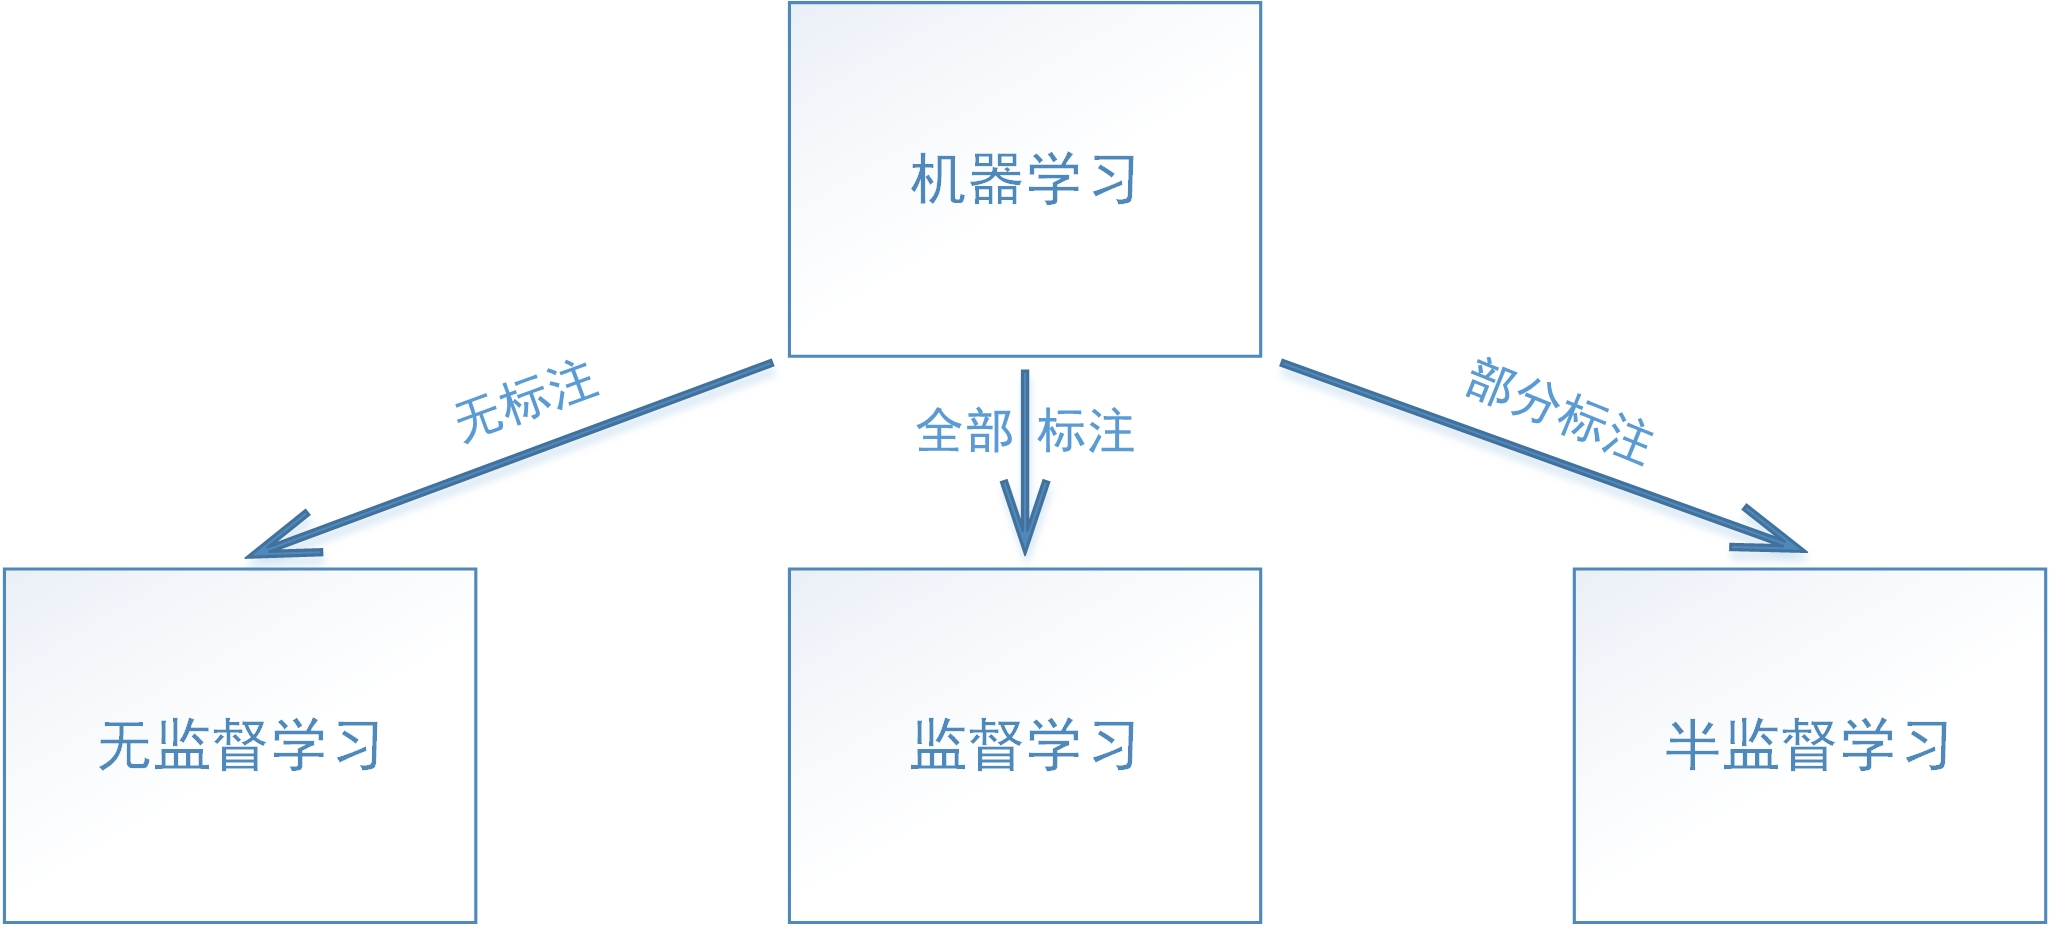
\includegraphics[width=0.8\linewidth]{Char1/机器学习.jpg}
    \caption{\label{Char1:fig:ML}三种机器学习类型。}
\end{figure}

虽然半监督学习算法可以从未标注数据中获取信息并以此增强算法的学习性能,然而实际数据中可能会出现更为苛刻的标注情况。
例如在已标注数据中,{由于标注者的兴趣倾向或搜集难度等客观因素},
数据的标签通常也是不完整的或是模糊不定的\cite{Garg_PU_2021,Fang_Partial_2019}。
一方面,在一些二分类问题的实际应用场景中,常常出现对单个类别某方向的偏爱倾向,
{即训练数据集中的标注数据部分只有少部分的正例数据被标注到。}
出现这种情况的原因往往是该场景下某些正例比较显眼或者突出以至于容易被标注,而反例却多种多样且难以甄别。
例如,在各种新闻媒体或商家点评等对内容真实性较为依赖的领域,对虚假新闻或虚假评论的检测是非常重要的,其中一些明显的虚假言论会被用户举报或被审核员注意到并标注为正,
然而许许多多难以辨别的言论仍然处于未知状态中\cite{Hsieh_PUscnario1_2015};
在Twitter或Tiktok等社交媒体中,对用户的可能友谊关系或者可能感兴趣的推荐是主要的关注方向,这些数据的正例标注可以通过用户现有的好友关系或点赞浏览记录得到,
但对于繁杂的负例标注信息却难以获得\cite{Jaskie_PUscnario3_2019};
其余诸如此类场景还有遥感高光谱图像或军事攻击的目标识别\cite{Li_PUscnario2_2010},医院住院时间规划\cite{Arjannikov_Empirical_2021}
和词汇情感分析\cite{Wang_Sentiment_2017}等。
另一方面,在多标签标注任务中,对所有类别标签进行精准的正负标注显然也是较为困难且昂贵的\cite{Deng_ML_2014}。
尤其是在潜在标签的数量较大时,人工标注不仅难以查全所有出现的类别,更难以为所有未出现的类别打上精确的负标签\cite{Cole_SML_2021},
如包含多个物体的目标识别场景、包含多种疾病类型的医学CT图像\cite{Redmon_YOLO_2017}和包含多种语义的文章\cite{Kenton_BERT_2019}等等。
{因此实际场景中,所需要识别的正例方面都是标注者高度感兴趣或容易甄别的而负例数据却是多样化或者缺失的,
同时相当比例的数据由于难以标注而处于未标注状态,这便产生了许多正例和无标注数据集(Positive and Unlabeled Dataset, PU数据)。}
在这些情况下,常规半监督学习表现欠佳,而基于PU数据集的正例无标注学习(Positive and Unlabeled Learning, PU学习)成为首选考虑\cite{Fusilier_PU_2015}。

此外,由于地理位置等因素的制约和个人存储通讯设备的普及,现代数据通常收集并存储在不同的数据节点中,并通过一定的连接关系互相进行通信或传输数据进行协同合作\cite{廖文龙_分布式半监督_2021}。
尽管现代通信网络的能力在逐年递增,但也对频繁的大规模数据交换显得力不从心,{同时直接传输原始数据也存在着泄露用户隐私的风险。}
为此,分布式信息处理,即通过各节点间的少量信息传递进行协作的信息处理方法,在许多领域受到了关注。例如,基于多个传感器分别收集数据的无线传感器网络\cite{Hua_Distributed_2015,Zhang_Distributed_2021},
互联网或科技企业中由多个计算集群组成的分布式计算机系统\cite{沈鹏程_分布式信息论_2016},
多地天文台组成的全时观测系统\cite{FAST}等等。

综上所述,尽管正例无标注学习在多个领域得到了充分地研究,但目前基于分布式场景的正例无标注学习却鲜有报道。本文将主要关注分布式场景下的正例无标注学习,探讨如何采用较少的信息传递,在分布式网络上使得存储着正例无标注数据的各独立数据节点得到一致性的最优模型,并给出相应的解决方案。

\section{国内外研究现状}
% Chapter 1.2.1
\subsection{半监督学习}
如上文所述,监督学习为了得到良好的分类效果,需要大量昂贵且难以获得的具有完备标注的数据集。
但在现实场景中{往往存在着大量}由部分有标注的数据和部分无标注的数据组成的数据集。
若是抛弃无标注数据仅使用标注数据进行监督学习算法的训练,则可能因为训练样本过少导致在训练过程中拘泥于少部分已标注数据,使得算法对于整个数据的泛化性能较差。
为了对数量可观的无标注数据加以利用,以便从少量标注数据和相当比例的未标注数据中获取对分类有利的信息,半监督学习作为一类可以降低标注量需求的重要算法受到了重视。
如\autoref{Char1:fig:semi-supervised1}所示,半监督学习的任务便是通过在此类被部分标注的数据中学习,并最终使得算法能够在未见数据上进行良好的分类效果。
鉴于半监督学习能够在使用少量珍贵的已标注数据的同时充分利用大量未标注数据,在节省标注资源以及成本的情况下取得较好的分类精度,近年来许多文献对半监督方向的算法进行了广泛的探讨和研究。
\begin{figure}[htbp]
    \centering
    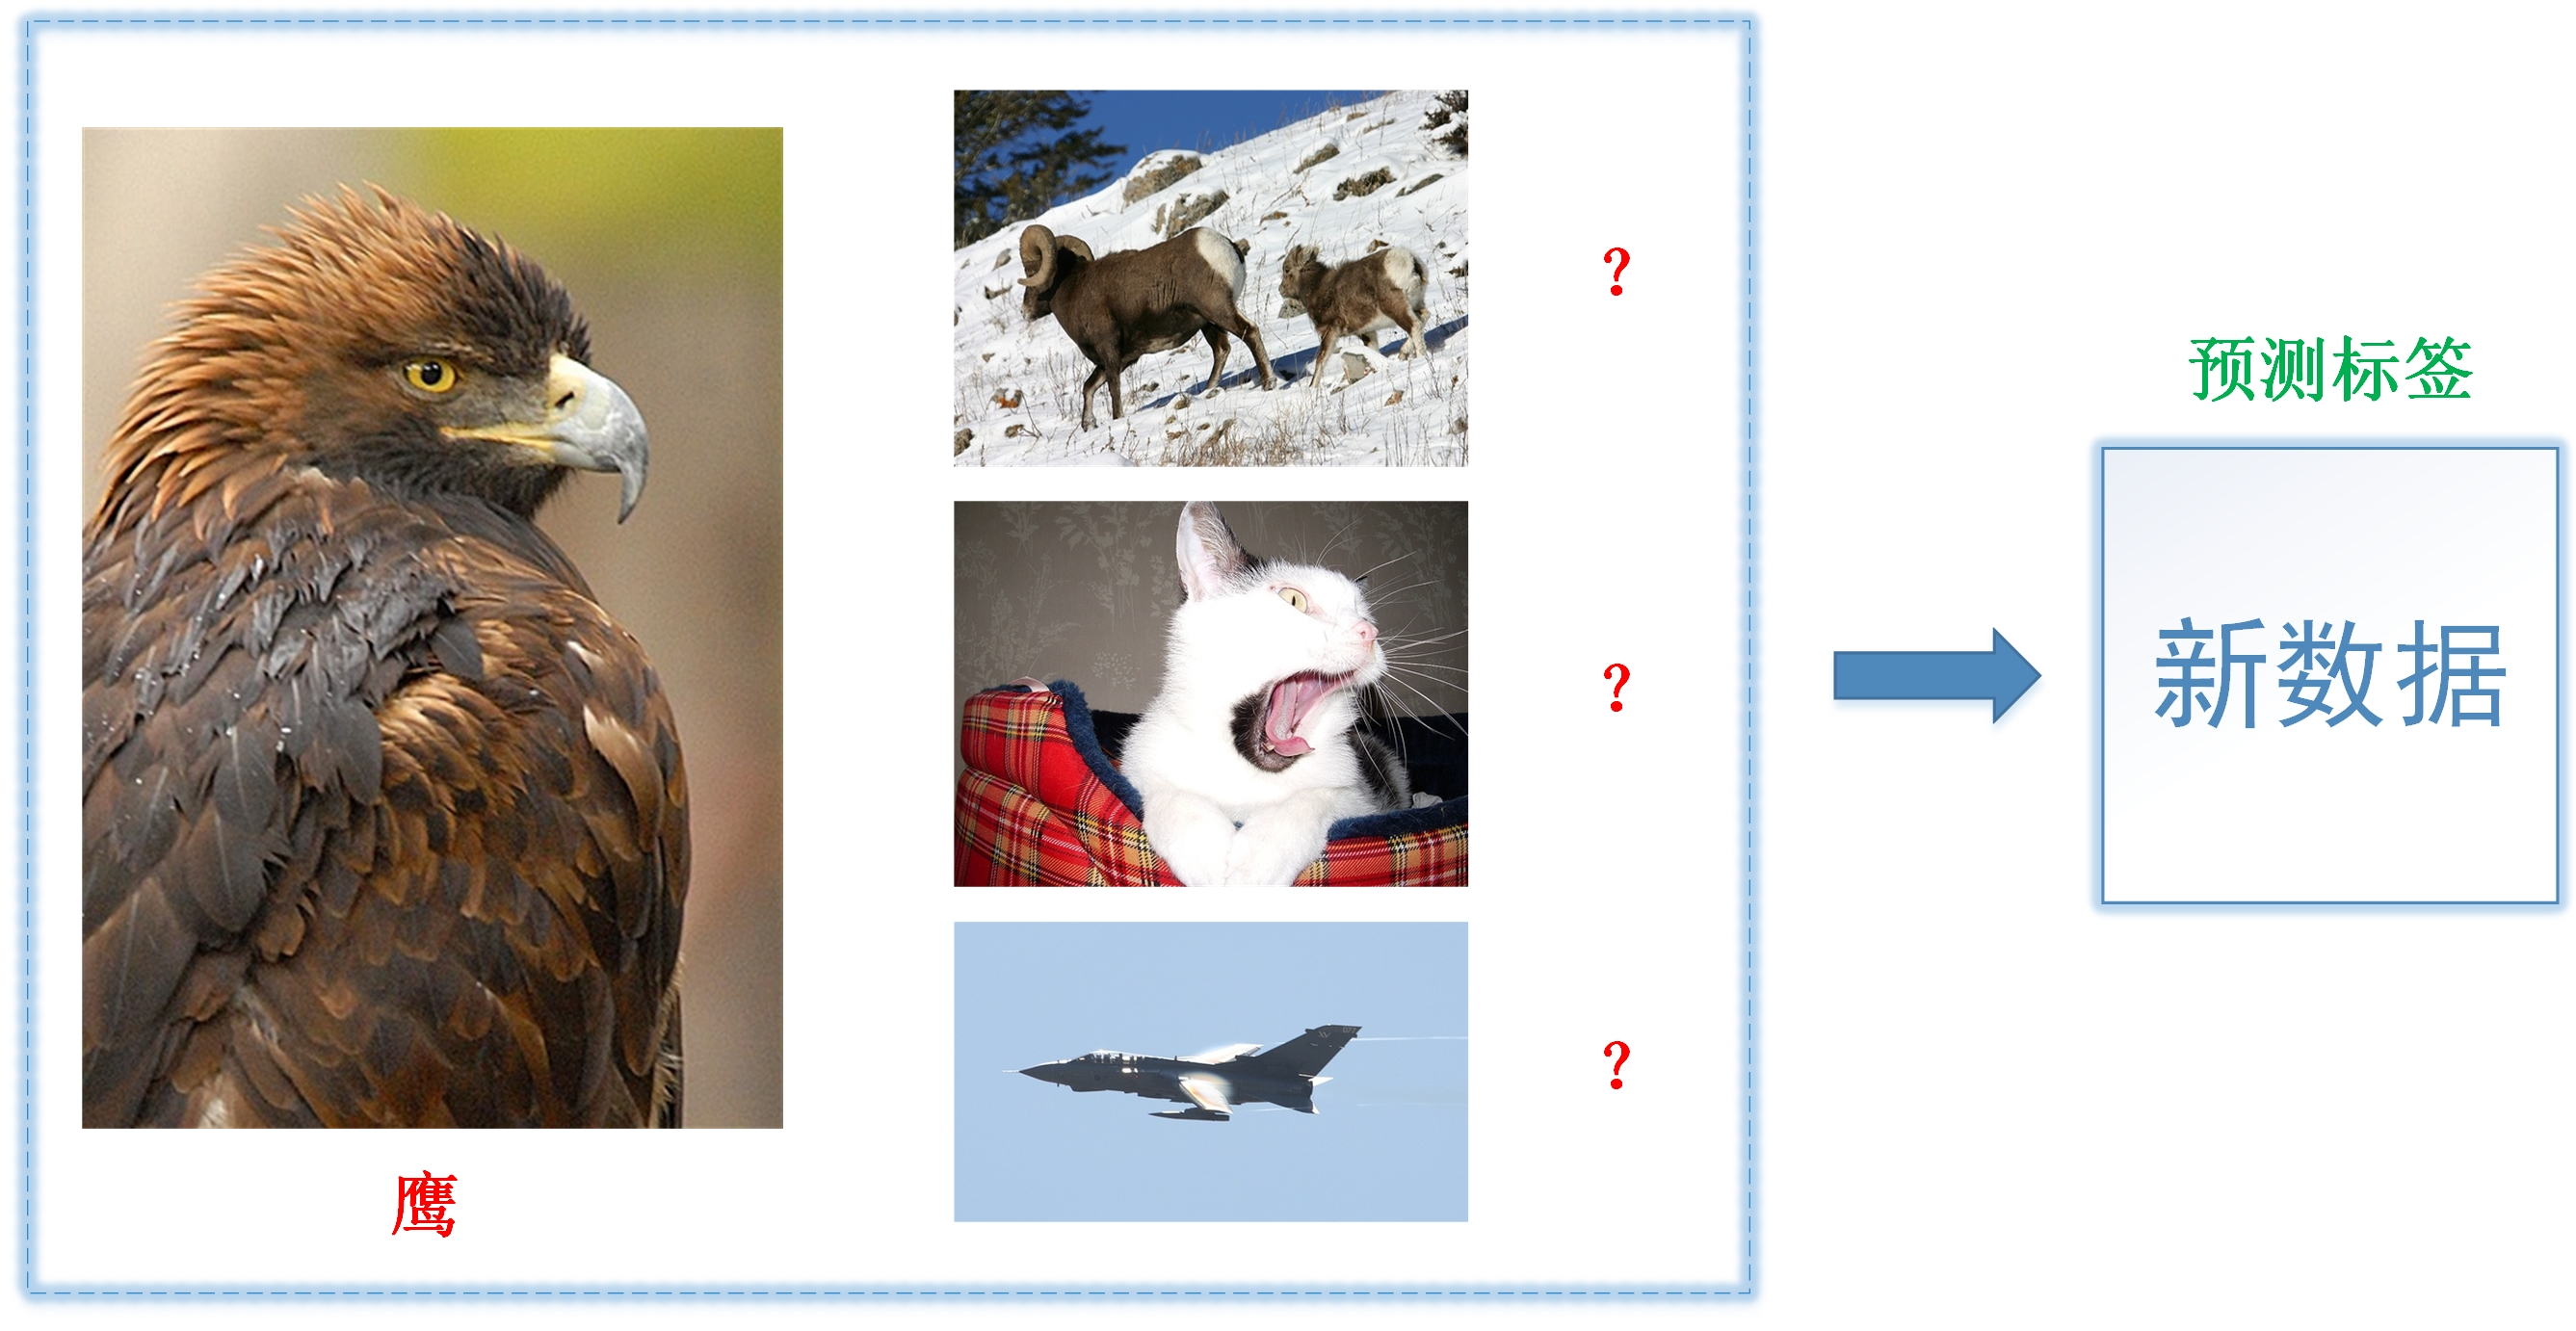
\includegraphics[width=0.8\linewidth]{Char1/半监督图1.jpg}
    \caption{\label{Char1:fig:semi-supervised1}一个半监督学习任务的例子。}
\end{figure}

% 从这里开始分几类探讨
对半监督学习算法的研究主要分为以下几类:
(1)基于潜在概率分布的生成式模型。该类方法通过对现有数据的分布进行概率假设,并期望所有数据都可以从特定概率模型中生成得到。利用期望最大化算法(expection maximization,EM)算法对所有未标注数据进行概率预估\cite{Zhang_Semi_2007,Ma_Semi_2017}。
但是这样的算法往往强烈依赖于其算法所假设的数据概率分布是否与真实概率分布相近,导致算法的性能难以保证。
(2)基于消歧策略或标签传播的直推式算法。
根据已有标注信息,对在未标注数据中可能存在的正例或者反例标签方案进行探索,
送入支持向量机(support vector machine, SVM)或其他分类算法中进行训练,
并最终选择一个使得算法表现最优的的标注方案\cite{Wang_Partial_2019, Wang_Semi-Supervised_2020,Li_Semi_2018}。
但在标注数据与未标注数据分布差异较大的时候,此类算法的性能会大打折扣。
(3)基于图模型的半监督学习。
基于对数据分布的平滑性假设,即相同聚类或相近稠密区域中的数据大概率属于同一类别,
算法便可根据各数据在流形图上的联系来学习数据之间的相关性\cite{Belkin_Manifold_2006,Huang_Semi_2014,Forestier_Semi_2016}。
其中流形约束主要通过在流形图中计算新数据与原有数据之间的距离函数,并通过最优化整个流形来确定未标注数据的归属\cite{Zhu_Manifold_2005,Zhu_Semi_2005}。
然而,此类算法基于图模型,对大规模数据集的存储空间和计算能力需求较高。
将流形约束的约束项结合各类半监督损失函数,
可以有效增强算法对未见数据的适应性,从而提升算法性能\cite{Van_SemiSurvey_2020, Dong_Semi_2016}。

% Chapter 1.2.2
\subsection{正例无标注学习}
如上文所述,即使半监督学习已经大大减少了对标注数据的需求,许多实际场景中已标注的数据仍然存在不完整的标注状态。
在许多涉及"Yes or No"的单标签二分类场景中,其中的正例方向往往较受关注以至于出现越来越多的正例和无标注数据(Positive and Unlabelled, PU)数据。
因此,可处理PU数据并从中学习到有效信息的PU学习备受关注,人们提出了许多PU学习算法,
它们主要分为以下几类:

{
(1)第一类算法从未标记数据集中选择一些可靠的数据作为负类数据,
然后同时使用正反两个示例将学习问题化为一个有监督的学习问题\cite{Youngs_SMD_2015,Luo_Simple_2017}。
显然,这种两步策略的表现高度依赖于识别的负训练数据的准确性,且识别的准确度不稳定。

(2)第二类算法将PU学习定义为标签噪声学习问题,该类方法是将未标记数据作为带有随机噪声的负面数据处理,即把原始的未标注正例视为被误分类到负例的数据\cite{Lee_WLR_2003}。
这种策略的缺点在于若未标注的正例比例过高,则噪声强度会急剧增大,导致算法效果收效甚微。

(3)第三类算法通过设计无偏损失函数将PU学习定义为代价敏感型学习问题,
并修改正负例损失函数的权重来学习\cite{Kiryo_Positive_2017}。
考虑到无标签数据的隐藏分布信息,如何设计合理的代价函数以高效地利用其中蕴含的丰富信息是提高分类性能的关键。为此,文献\parencite{Gong_Margin_2018}提出了基于最大化输出正负类间隔的间隔损失函数来学习隐藏分布信息。
文献\parencite{Gong_LLSVM_2019}中提出了一种大间隔标签校准支持向量机
(large-margin label-calibrated support vector machines,LLSVM),
该支持向量机使用标定后的标签来扩大正负类之间的间隔。}
该方法虽然对PU数据具有较好的分类性能,但在标记正例率较低的情况下仍表现欠佳,或难以处理复杂的非线性分类问题。

% SML
此外在多标签学习领域,一张图片可能有多个标签类需要预测,而要完全的标注所有标签类的正负是困难的,因此基于上述标注者对正类的偏爱可能会出现大量仅有部分正例标签被标注的多标签数据\cite{Cole_SML_2021,Han_PUMulti_2018}。
基于多标签PU数据的上述性质,在多标签PU学习中除了要考虑生成模型\cite{Chu_PUML_2018}、
假负噪声标签\cite{Mac_PUML_2019,Sun_PUML_2010}和代价敏感型探索正例数据和未标注数据之间的关系外,还需要考虑多个标签之间的关系,使用标签矩阵或标签平滑等方式从中获取标签之间的相关信息以提升学习性能\cite{Hsieh_PUscnario1_2015,Szegedy_LabelSmooth_2016}。

% 本文我们使用标注标签部分的损失函数$l_+\left(\boldsymbol f_i, \boldsymbol y_i\right), \boldsymbol y_i=+1, i\in\mathcal{L}$,
% 而需要对未标注标签部分设计损失函数$l_\varnothing\left(\boldsymbol f_i, \boldsymbol y_i\right), 
% \boldsymbol y_i=\varnothing, i\in\mathcal{L}$来约束输出类别的分布,来防止算法被单正例标签支配以至于在所有数据上
% 该类都输出为正,其中$\mathcal{L}=\left\{1,2,...,L\right\}$表示共有$L$个标签的标签集。
% 在一个单正例标注的数据上应用上述损失函数,则算法模型可写为:
% \begin{equation}
%     \label{equ1:Labeled&Unlabeled}
%     \min \sum_{i\in\mathcal{L}}l_+\left(\boldsymbol f_i, \boldsymbol y_i\right)
%     +l_\varnothing\left(\boldsymbol f_i, \boldsymbol y_i\right)
% \end{equation}
% 其中前半部分通常可以使用常见的监督学习损失函数例如SVM的合页损失函数(Hinge Loss)或二元交叉熵损失函数(binary cross-entropy,BCE)。
% 后半部分$l_\varnothing\left(\boldsymbol f_i, \boldsymbol y_i\right), \boldsymbol y_i=\varnothing$可
% 根据实际应用场景转换为不同的损失函数去约束输出。
% 在单标签PU学习领域中$\mathcal{L}$简化为$\left\{1\right\}$,可使用的通过最大化正向输出与负向输出间隔以增加算法鲁棒性的的最大间隔损失\cite{Gong_Margin_2018}
% 和通过约束输出的门限将算法从正向损失的束缚中解脱出来的标签校准损失\cite{Gong_LLSVM_2019}等。
% 在多标签PU学习可用到的通过改变真实标签分布来约束输出强直性的标签平滑损失项\cite{Szegedy_LabelSmooth_2016}
% 或通过对输出正项数量的期望值进行固定来迫使算法输出少量相关正向标签的正向标签数量约束项\cite{Durand_EPR_2019}等。

% 1.2.3
\section{分布式信息处理}
在基于现代网络的大数据时代,数据往往存储于地理位置不同的本地数据存储中心中,
考虑隐私及通信带宽的限制,往往期望在不传输原始数据或仅传输少量信息的条件下对全局问题进行优化并使各节点得到一致的全局最优解。
然而现有半监督学习或正例无标注方法大多属于集中式运算,即所有的训练数据都必须集中到一个数据中心进行处理。
若是将所有独立节点的原始数据都传输到一个处理中心进行计算处理,不仅要考虑数据隐私方面的限制,而且从通信代价考虑也是不经济的。

通常情况下,对于集中式算法,我们需要设计一个损失函数$l\left(\boldsymbol F, \boldsymbol Y\right)$并通过将其最小化来获得输出最接近真实标签值的模型,
其中$\boldsymbol F$和$\boldsymbol Y$分别为包含数据中心所有数据的模型预测输出和真实标签的矩阵。
而分布式算法则期望通过联合所有节点的损失函数,组成全局最小化问题并得到全局最优解,即:
\begin{equation}
    \label{Char1:equ:distributed}
    \min \sum_{j\in\mathcal{J}} l\left(\boldsymbol F_j, \boldsymbol Y_j\right),
\end{equation}
其中$\mathcal{J}=\left\{1,2,...J\right\}$为节点数为$J$的节点集,
$\boldsymbol F_j$和$\boldsymbol Y_j$分别为包含各节点所有数据的模型预测输出矩阵和真实标签矩阵。
如何通过分布式网络间的少量信息传递进行多节点之间的网络协同,高效地求解式\eqref{Char1:equ:distributed}并得到一个全局最优解,是分布式信息处理算法的主要任务。


\begin{figure}[htbp]
    \centering
    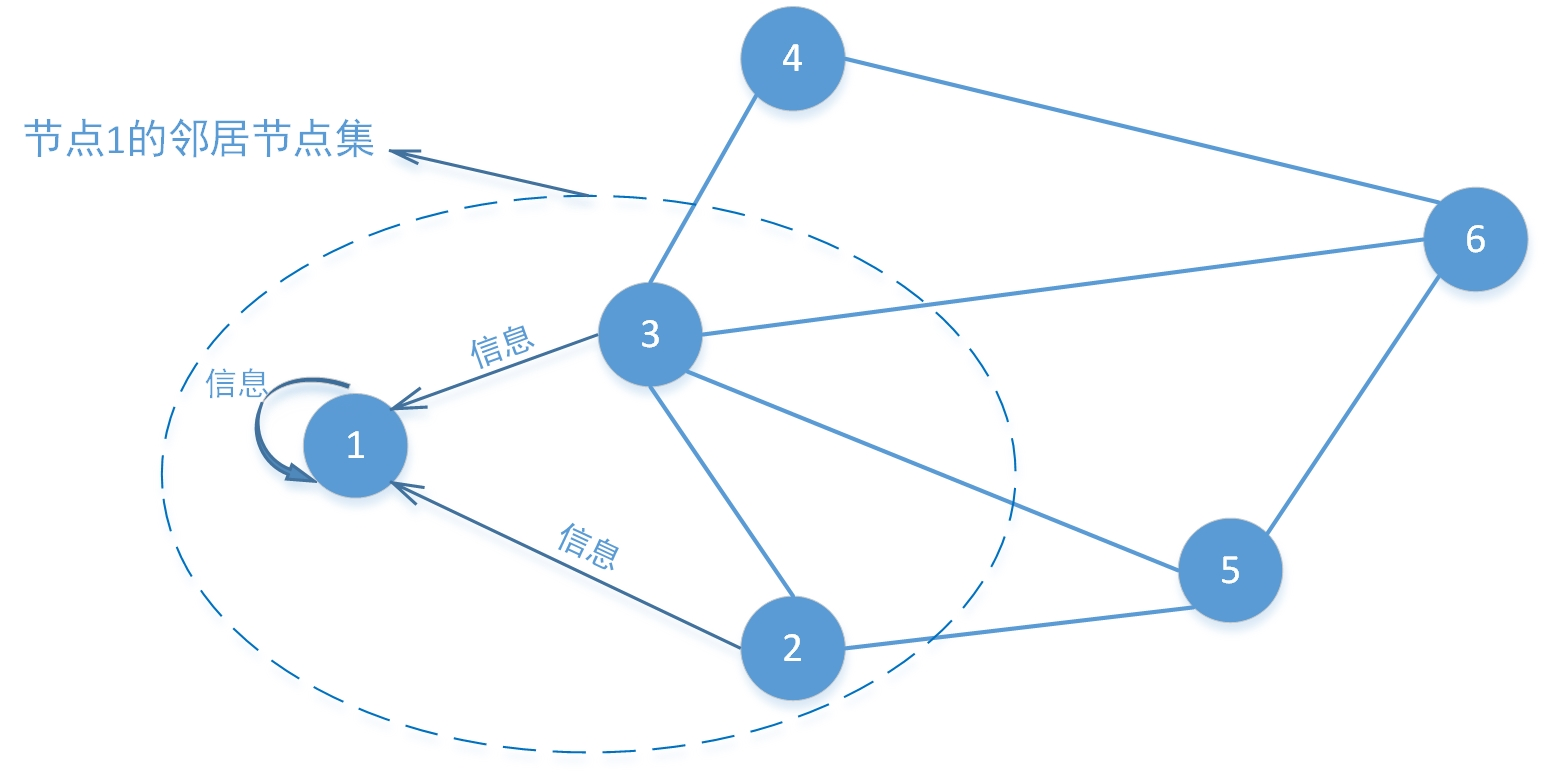
\includegraphics[width=0.85\linewidth]{Char1/分布式网络图1.jpg}
    \caption{\label{Char1:fig:distributed}分布式网络中的节点示意图。}
\end{figure}

目前已有许多的分布式算法被相继提出并在不同领域上进行应用,有基于SVM进行分布式优化的分布式支持向量机\cite{Lu_DistributedSVM_2016,Liu_SemiSVM_2018,Scardapane_Distributed_2016, Hou_hdsvm_2017}、分布式的聚类算法\cite{Kotary_distributed_2020}、以分布式账本计算为基础的区块链技术\cite{Kuo_BlockChain_2017}、分布式异常检测\cite{Miao_Distributed_2018}和分布式贝叶斯算法\cite{Hua_Distributed_2015}等等。
分布式节点处理不似集中式处理那般将所有数据都传输至一个数据中心进行存储或计算,而是每个节点都承担一定的存储和计算任务。{如\autoref{Char1:fig:distributed}所示,数据节点1仅与其邻居节点进行局部通信并通过网络交换共享关键信息使得信息在全局网络中传递。}
相比于集中式算法,分布式算法的主要优点有:

(1)更好的鲁棒性。网络中并非只仰赖一个单独的计算存储中心,而是使用多个分布在不同区域的单独计算存储节点。
若是其中一个节点发生故障,其余节点仍然可以相互传递信息,对总体所造成的不良影响较小,增强了网络的稳定性和健壮程度\cite{Miao_Distributed_2018}。

(2)通过将总体任务分散到各个节点,有效地利用分布在各地各设备的计算能力。
各节点先使用本地算力对数据进行各式预处理之后,在本地通过损失函数的反向传递计算好梯度或中间变量等信息后,
通过网络将这些信息传递到邻居节点\cite{Verbraeken_Survey_2020}。
相比于单一数据中心对所有数据进行计算,分布式网络对分散算力的利用更为充分。

(3)更小的通信压力以及更好的隐私保护。
相比于集中式所需要的整体数据传递存储,分布式仅仅通过网络传递由本地数据计算得来的少量信息,即可得到与集中式相等或接近的全局最优解\cite{Scardapane_Distributed_2016}。
并且节点之间不直接传递原始数据,从一定程度上对数据的隐私性进行了保护\cite{Shen_Distributed_2014}。

{分布式算法所拥有上述多种优点使其成为现代信息处理的热门研究方向,但基于正例无标注数据的分布式机器学习研究仍然寥寥无几,大部分正例无标注学习仍然需要将所有数据传输至单一数据节点进行集中式计算。}

\section{本文研究内容与结构安排}
\subsection{本文研究内容与创新点}
{本文考虑实际场景中仅有部分正例数据被标注的场景,同时这些数据资源分布式地存储在地理位置不同的分布式节点中,主要研究了基于正例无标注数据的分布式学习算法,分别针对单标签的正例无标注学习问题和多标签的单正例无标注学习问题展开研究,提出了相应的分布式正例无标注学习算法,并进一步通过考虑分布式情况的最坏扰动,对提出的两种算法进行优化。}
本文的主要研究内容和创新点如下:

(1)提出了一种基于交替乘子法的分布式正例无标注学习算法。
在分布式网络上构建各节点的本地损失函数,并通过随机特征映射逼近非线性核函数以实现分布式场景下的核函数计算。对标注数据使用合页损失函数(hinge loss),并对未标注数据进行输出放大约束以及带自适应门限的标签校准约束。此外,引入流形约束进一步提升半监督学习性能,并使用锚数据点实现该流形约束的去中心化处理,使得通过少量信息交换,本地流形约束可以逼近全局最优性能。
通过交替乘子法解决基于一致性约束的全局优化问题得到全局最优解。
最后,通过与其余正例无标注学习算法在不同标注率的不同数据集上的性能对比,证实了本文提出的基于交替乘子法的分布式正例无标注学习算法的优越性。

(2)提出了一种基于事件触发的分布式半监督单正例多标签学习算法。
对于未标注数据和只含一个正例标注的单正例多标签数据,探索了几种不同的损失函数,使得算法能够在标注数据量较少情况下获得较好的多标签分类性能。通过分布式梯度下降算法以及事件触发机制对上述损失函数进行分布式优化,在获得全局最优解的同时大大减少了各节点之间网络的通信代价。
最后在多个图像数据集上证实了两种损失函数的优越性,即使在更极端的标注条件下,仍取得相较于其他类似算法更优越的性能。

(3)对上述两种算法的基础结构进行分布式全局最坏扰动,在仅有少量正例标注的情况下进一步提升算法的性能。通过最差噪声扰动和最坏连接扰动的结合,以及使用锚点数据使得本地扰动逼近全局最坏扰动的策略,上述两类算法都在相同标注量的相同数据集上取得了更进一步的性能优化。

\subsection{本文结构安排}
\begin{figure}[htbp]
    \centering
    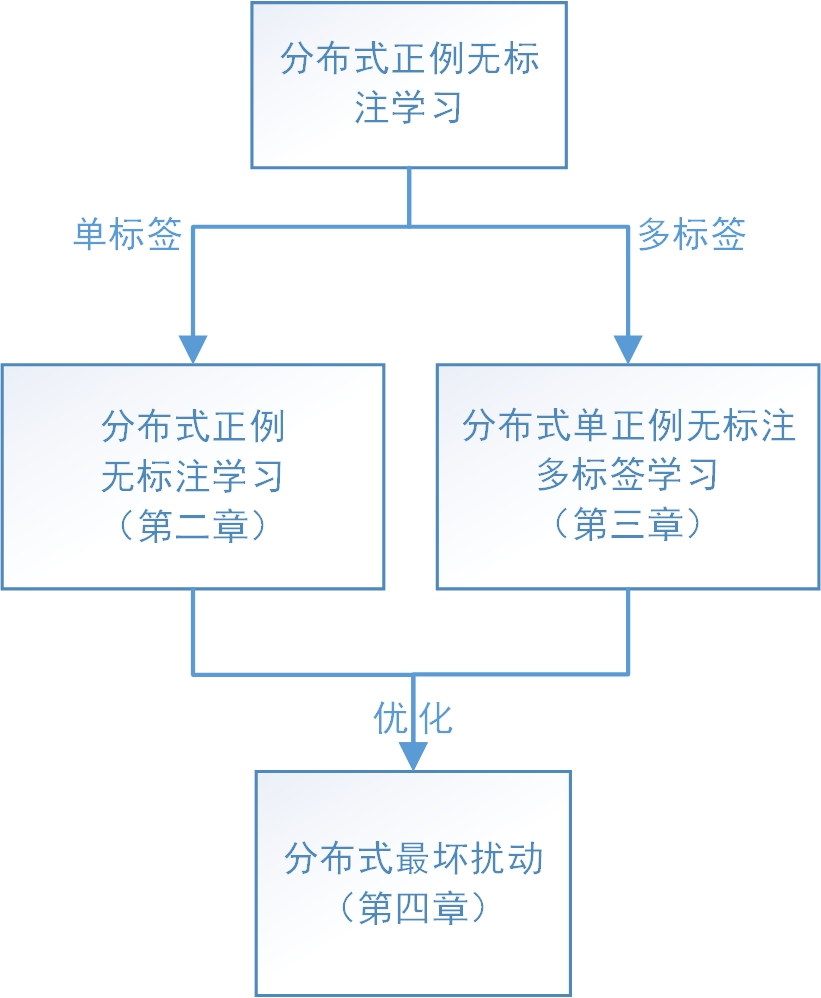
\includegraphics[width=0.5\linewidth]{Char1/本文结构.jpg}
    \caption{\label{Char1:fig:structure}本文的结构安排。}
\end{figure}
本文研究内容及其结构安排如\autoref{Char1:fig:structure}所示。具体各章节结构安排如下:

在第一章中,本文介绍了本文的研究背景以及意义,对正例无标注学习以及分布式信息处理进行了简要的概述,并阐明了本文的研究内容以及创新点。

在第二章中,本文首先对本地节点提出适用于正例无标注数据的去中心化单标签分类损失函数,然后提出全局优化问题,再通过交替乘子法对全局损失函进行优化取得全局最优解。

在第三章中,本文探索两种适用于无标注数据和单正例多标签数据的去中心化损失函数并提出全局优化问题,使用分布式梯度下降算法对全局损失函数进行优化,并借助事件触发策略减少了各节点间的网络通信的频率。

在第四章中,本文介绍了两种最坏扰动机制,并通过锚点数据策略将其推广至分布式全局最坏扰动,结合第二章和第三章的内容对正例无标注算法进行性能优化。

在第五章中,本文对本文的研究内容进行了归纳总结,并对现有的不足之处和未来的研究方向进行了展望。


% Chapter 2
\chapter{分布式正例无标注学习}
% Chapter 2.1
\section{引言}\label{Char2_Pre}
{在单标签分类中,对于每一个数据$\boldsymbol x_n$都有一个相应的标签$y_n\in\left\{1,0\right\}$表示其所属类别是正类还是负类。
但在正例无标注学习(positive and unlabeled learning,PU learning)中,
出于对正例标注的偏好以及负例标注的困难,每个数据$\boldsymbol x_n$可能处于正例标注或者未标注状态,}
即其观测标注为$z_n\in\left\{1,\varnothing\right\}$,其中$\varnothing$可能为正类也可能为负类。
{此外,出于地理位置、数据隐私性和网络通讯代价的考虑,数据通常存储在不同的数据节点中。}
我们的目的是针对正例无标注数据分布于不同节点的情况,通过分布式网络中的少量信息传递,训练得到一个使得全局分类效果最优的分类器。
{为此,在本章中,我们考虑了正例无标注数据存储在不同分布式节点的场景,提出了基于正例无标注数据的分布式学习算法。}

本章剩余部分的简介如下:
在\ref{Preliminaries}节中简要介绍了一些预备知识,即随机特征映射和流形约束。
在\ref{LossDesign}节,根据各节点的正例无标注数据构建了去中心化的损失函数并提出了全局优化问题。
{在\ref{Distributed}节,对全局优化问题使用交替乘子法进行分布式优化完成分布式正例无标注算法,并对其收敛性进行了分析。}
在\ref{Experiments}节,利用若干模拟及真实数据集对提出的算法进行了测试,并通过与其他算法的对比证实其优越性。
\ref{Summary}节,对本章的工作做出了总结。

\section{预备知识}\label{Preliminaries}
在分布式场景中,考虑到各节点之间不希望传输原始数据信息,往往难以实现基于数据对的核函数的计算。文献\parencite{Yuan_Efficient_2015,Vedaldi_Efficient_2012,Vempati_Generalized_2010}
对通过随机映射逼近核函数高维空间的随机特征映射算法进行了探索研究。此外,在图半监督学习中,流形约束是一种典型的图半监督学习算法,可以有效提升半监督学习的效果\cite{Van_SemiSurvey_2020, Dong_Semi_2016}。
因此,为了使本文自我包含,在本节中将首先对基于正例无标注数据的分布式学习算法所需要的预备知识点,随机特征映射和流形约束进行简单的介绍。

\subsection{随机特征映射}\label{char:RFM}
% 在分布式优化时,由于节点之间不期望传输原始数据,所以在本地节点通过随机特征映射的形式将数据映射到高维核函数空间上去,
% 并在本地节点计算loss和反向传播的梯度等信息,
% 则节点间仅需少量的信息传递便可以达到核函数的非线性效果。
% 同时也需要锚点数据集来使本地流形约束的效果逼近全局流形约束。
许多著名的分类算法如支持向量机(support vector machine,SVM)或逻辑回归(Logsitic Regreesion,LR)等,往往使用核函数$\kappa\left(\cdot, \cdot\right)$来构建非线性判别函数公式,如:
\begin{equation}
    \label{classifier_kernel}
    \begin{split}
        f(\boldsymbol w|\boldsymbol x)
        &=\sum_{n \in \mathcal{N}} a_{n} \kappa\left(\boldsymbol x_{n}, \boldsymbol x\right)+b\\
        &\triangleq \boldsymbol w^{T} \boldsymbol \phi(\boldsymbol x)+b,
    \end{split}
\end{equation}
其中$\mathcal{N}=\left\{1,2,...,N\right\}$代表$N$个数据的序号集,$a_n$为权重系数;
$\boldsymbol{w} =\sum_{n \in \mathcal{N}}a_n {\boldsymbol\phi^T(\boldsymbol{x}_{n})}$为参数向量,且$\boldsymbol\phi\left(\boldsymbol{\cdot}\right)$即为原始数据$\boldsymbol{x}_{n}$在核函数的重构希尔伯特空间(RKHS)
的非线性隐式映射。由于$\boldsymbol\phi\left(\boldsymbol{\cdot}\right)$是未知且难以获得的,$\boldsymbol w$无法直接计算。因此核函数的使用通常是如式\eqref{classifier_kernel}般通过内积进行计算。但是,这在分布式场景下是无法实现的,因为考虑到隐私和通信成本,不希望在邻居节点之间直接传输原始数据。

为了解决这一问题,人们提出随机逼近的思想,即对隐式高维核映射$\boldsymbol\phi\left(\boldsymbol{\cdot}\right)$通过随机采样进行近似,称之为随机特征映射(random feature maps,RFM)。
它通过随机抽样将每个原始数据$\boldsymbol{x}_{n}$的原始空间$\mathbb{R}^d$映射到更高维度的空间$\mathbb{R}^D$
(一般来说$D>d$) \cite{Yuan_Efficient_2015}。
目前,许多非线性核的随机逼近方法已经被提出,本文选择使用可加性核$\chi^2$,
因其可在保持良好性能的同时大幅降低所需要拓展的维度$D$\cite{Yuan_Efficient_2015,Vedaldi_Efficient_2012}。

在可加性核随机映射中,原始数据$\boldsymbol{x}_{n}$的每个元素如第$d_i$个元素$\boldsymbol{x}_{n\left(d_i\right)}\left(d_i=1,2,..,d\right)$首先被放缩至$\left[0,1\right]$,
再根据特征函数进行间隔为$L$的$2S+1$次采样,得到单个元素的映射向量$\hat{\boldsymbol\phi}\left(\boldsymbol{x}_{n\left(d_i\right)}\right)$。
将单个元素的映射向量的单个采样值记为$\hat{\boldsymbol\phi}\left(\boldsymbol{x}_{n\left(d_i\right)}\right)_{\left(s\right)}\left(s=0,1,...,2S\right)$,
则$\chi^2$核对应于单个元素的随机特征映射计算如下:
\begin{equation}
    \label{RFM}
    \begin{split}
		\hat{\boldsymbol\phi}\left(\boldsymbol{x}_{n\left(d_i\right)}\right)_{(s)} = 
		\left\{ \begin{array}{l}
		\sqrt {{\boldsymbol{x}_{n\left(d_i\right)}}L{\mathop{\rm sech}\nolimits} \left( 0 \right)} 
        ~~~~~~~~~~~~~~~~~~~~~~~~~~~~~~~~~~~~~~~~~~~~~~~~~~~s = 0\\
		\sqrt {2{\boldsymbol{x}_{n\left(d_i\right)}}L{\mathop{\rm sech}\nolimits} \left( {\frac{{s + 1}}{2}\pi L} \right)}
        \cos \left( {\frac{{l + 1}}{2}L\log {\boldsymbol{x}_{n\left(d_i\right)}}} \right)~~~~~s > 0, odd\\
		\sqrt {2{\boldsymbol{x}_{n\left(d_i\right)}}L{\mathop{\rm sech}\nolimits} \left( {\frac{s}{2}\pi L} \right)} 
        \sin \left( {\frac{l}{2}L\log {\boldsymbol{x}_{n\left(d_i\right)}}} \right)~~~~~~~~~~~~~s > 0, even,
		\end{array}\right.
	\end{split}
\end{equation}
得到的映射向量$\hat{\boldsymbol\phi}\left(\boldsymbol{x}_{n\left(d_i\right)}\right)$进行竖向堆叠即可得到原始数据的特征映射向量
$\hat{\boldsymbol\phi}\left(\boldsymbol{x}_n\right)= {\left[{\hat{\boldsymbol\phi}\left(\boldsymbol{x}_{n\left(1\right)}\right)},\dots,{\hat{\boldsymbol\phi}\left(\boldsymbol{x}_{n\left(d\right)}\right)}\right]}$, 
其为隐式映射$\boldsymbol\phi\left(\boldsymbol{x}_n\right)$的近似逼近。

为表示方便,在下文中我们将基于随机特征映射得到的随机特征向量$\hat{\boldsymbol\phi}\left(\boldsymbol{x}_n\right)$扩展为
$\overline{\boldsymbol\phi}\left(\boldsymbol{x}_n\right)=\left[\hat{\boldsymbol\phi}\left(\boldsymbol{x}_n\right),1\right]$
,并简化参数$\boldsymbol\theta=\left[\boldsymbol w,b\right]$,则相应地式\eqref{classifier_kernel}可被重写为:
\begin{equation}
    \label{classifier_RFM}
    f\left(\boldsymbol\theta|\boldsymbol x_n\right)={\boldsymbol{\theta}}^T\overline{\boldsymbol\phi}\left(\boldsymbol{x}_n\right).
\end{equation}
在计算好判别函数$f\left(\boldsymbol x_n\right)$之后,标签就可以通过$y_n=\mathrm{sgn}\left(f\left(\boldsymbol\theta|\boldsymbol x_n\right)\right)$计算得到。
最终映射后的维度$D=\left(2S+1\right)d+1$。
{随机逼近的效果依赖于映射维度$D$的大小,通常情况下映射后的数据维度$D$越大,随机逼近的效果越接近原始核函数的效果\cite{Gerace_D_2020}。}

% Char 2.1.2
\subsection{流形约束}\label{Sec:ManifoldRegularization}
{在基于图的半监督学习中,一般假设数据分布满足平滑性假设,即属性相似的的样本大概率拥有相同真实标签值\cite{Belkin_Manifold_2006},且在相近稠密区域中(流形中)的数据标签值会倾向于拥有相近的标签\cite{Huang_Semi_2014,Forestier_Semi_2016}。}
为了改进算法对未见数据的泛化性能,流形正则化方法被提出并进行了深入研究,其将已被标记的数据作为“源”,
并据此生成一个具有最小边集的图\cite{Zhu_Semi_2003,Zhu_IntroductionSemi_2009}。
然后,可以通过比较新数据与源数据的距离函数使用该图对未标记数据进行分类,如\autoref{fig:graph}所示,
相比于已标注数据$\boldsymbol x_2$,新数据$\boldsymbol x_3$更受与其在图距离上更近的$\boldsymbol x_1$影响。
流形约束可以被描述为:
\begin{equation}
    \label{manifold_regularization}
    \min\frac{1}{2}{\sum\limits_{n,m}
    {\omega_{nm}\left[f\left(\boldsymbol{x}_n\right)-f\left(\boldsymbol{x}_m\right)\right]} ^2},
\end{equation}
其中${\omega_{nm}}=e^{\left(-\frac{\left\|\boldsymbol x_n-\boldsymbol x_m\right\|}{2}\right)}$表示距离函数。
\begin{figure}[htbp]
    \centering
    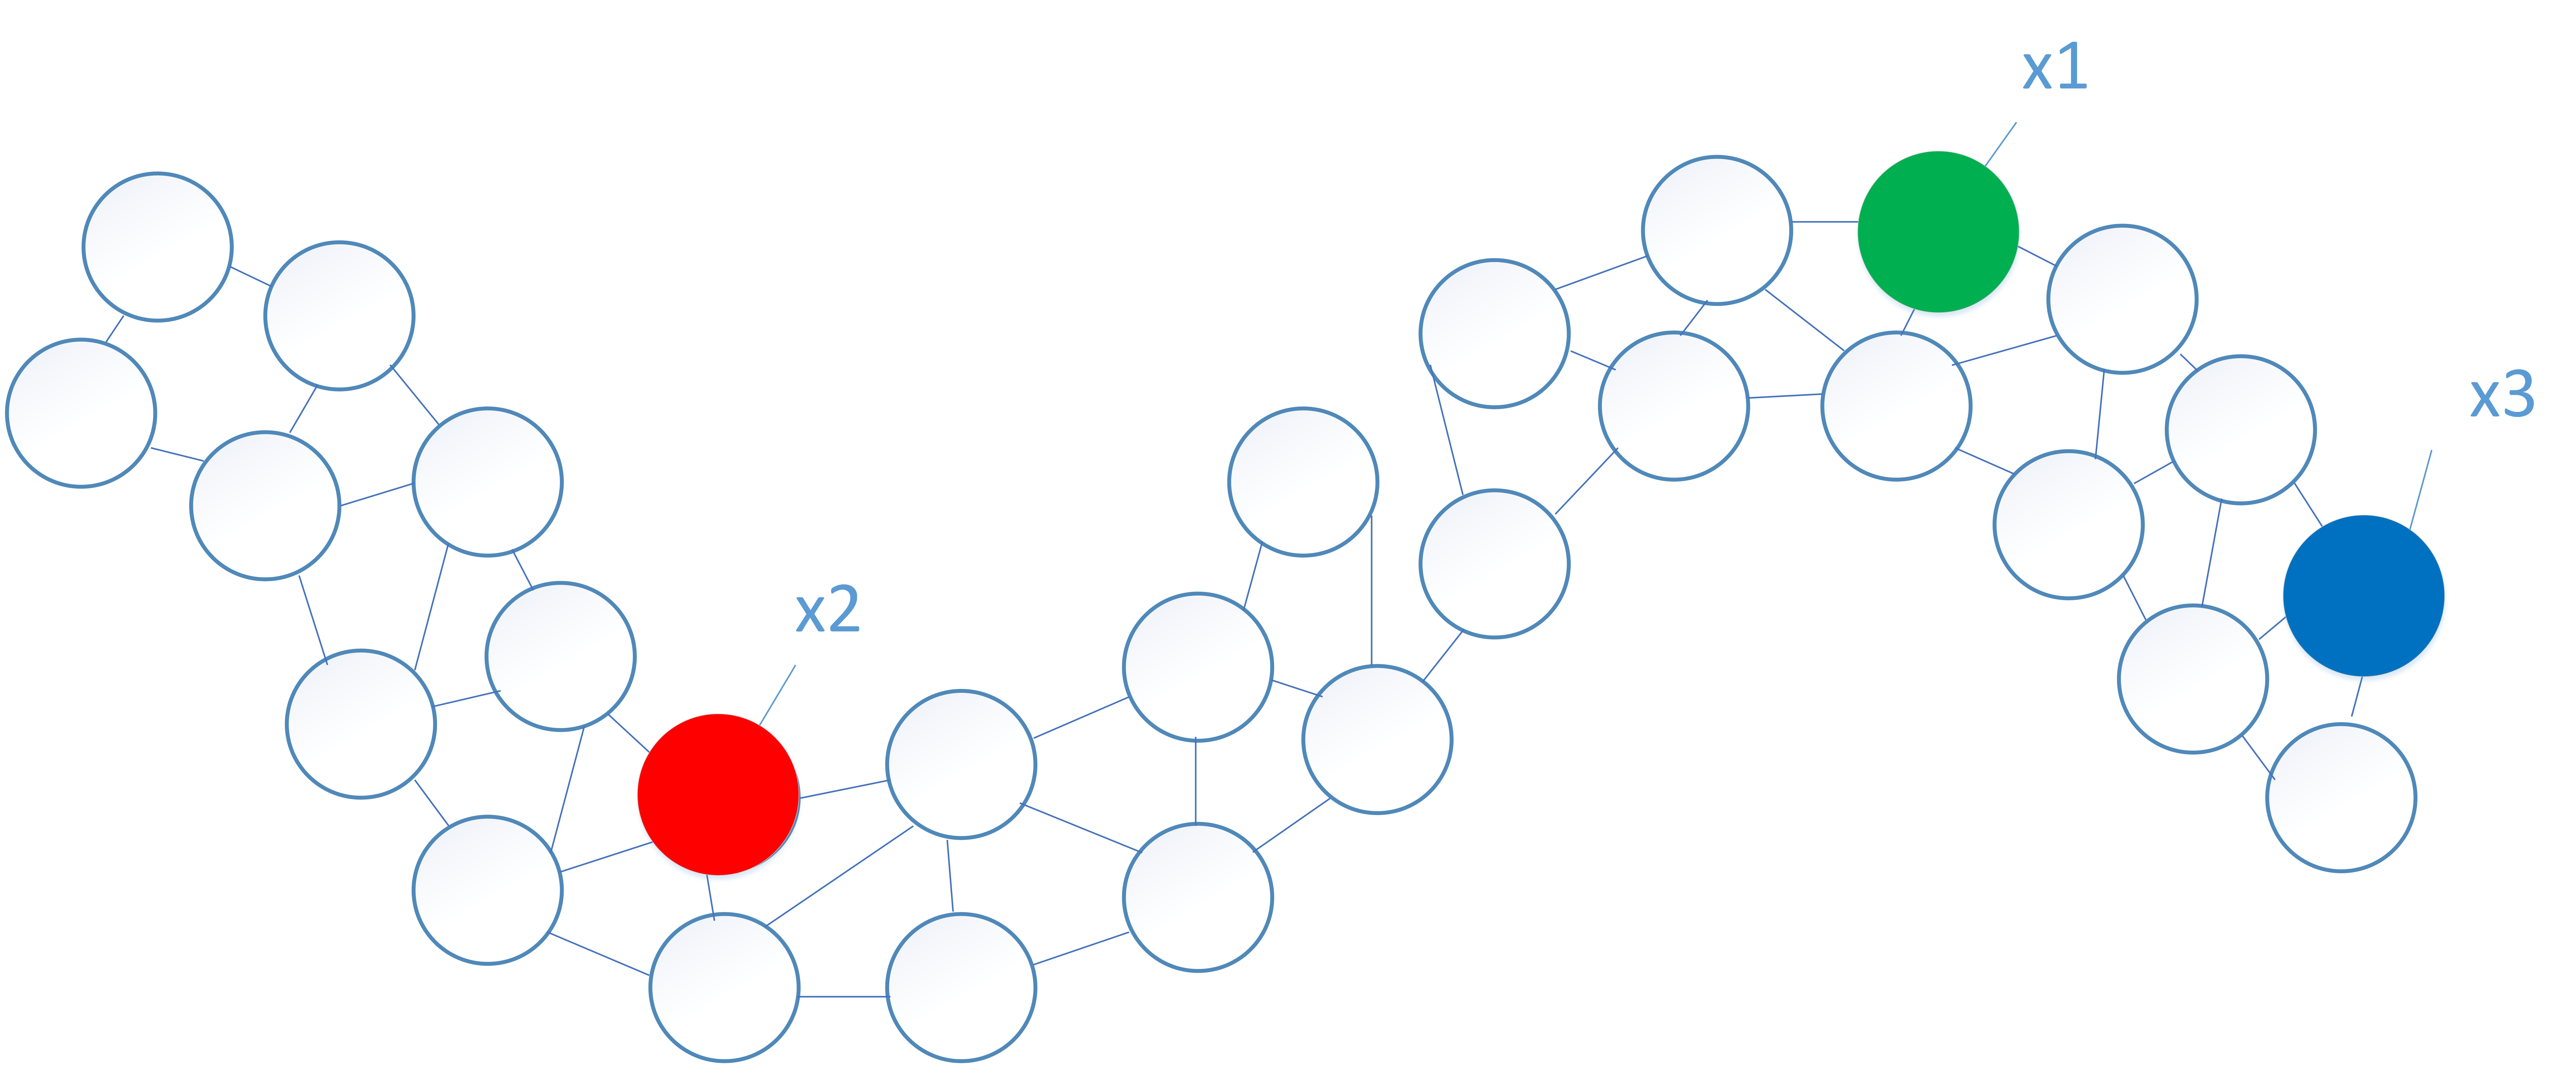
\includegraphics[width=0.85\linewidth]{流形图.jpg}
    \caption{\label{fig:graph}{数据流形图示意图}}
\end{figure}

% Char 2.2
\section{带自适应门限的正例无标注学习}\label{LossDesign}
{考虑一个有$J$个分布在不同地理位置的节点的分布式网络,网络可以通过无向图$\mathcal{G}=\left\{\mathcal{J},\mathcal{B}\right\}$表示,
其中$\mathcal{J}=\left\{1,2,...,J\right\}$表示节点集,$\mathcal{B}=\left\{\mathcal{B}_j\right\},j\in\mathcal{J}$
表示各节点的邻居节点的编号集,$\mathcal{E}=\left\{\left(j,b\right)\right\},j\in\mathcal{J},b\in\mathcal{B}_j$表示节点$j$的与邻居节点的边集。
在每个节点$j$中,都存储着$N_j$个数据,编号集记为$\mathcal{N}_j=\left\{1,2,...,N_j^p+N_j^u\right\}$,
其中$N_j^p$为正例数据个数,其编号集为$\mathcal{N}_j^p=\left\{1,2,...,N_j^p\right\}$,观测标注为$z_n=1,n\in\mathcal{N}_j^p$;
$N_j^u$为未标注数据个数,其编号集为$\mathcal{N}_j^u=\left\{N_j^p+1,N_j^p+2,...,N_j^p+N_j^u\right\}$,观测标注为$z_n=\varnothing,n\in\mathcal{N}_j^u$。
基于上述分布式网络,本节将在各个节点上根据正例无标注数据来构建对应的各节点的去中心化损失函数。}

针对\ref{char:RFM}节中所描述的分布式场景下构建非线性的困难,本文首先对每个节点的数据应用如式\eqref{RFM}的随机特征映射计算式,将其映射到$D$维空间上去,并记为$\boldsymbol \varPhi_j= \left\{\overline{\phi}\left(\boldsymbol x_n\right)\right\},n\in\mathcal{N}_j$,
且将标注正例部分和未标注部分分别记为$\boldsymbol \varPhi_j^p= \left\{\overline{\phi}\left(\boldsymbol x_n\right)\right\},n\in\mathcal{N}_j^p$
和$\boldsymbol \varPhi_j^u= \left\{\overline{\phi}\left(\boldsymbol x_n\right)\right\},n\in\mathcal{N}_j^u$。
在损失函数的设计上,首先对标注正例部分的数据应用基于SVM合页损失(hinge loss)的变种:
\begin{equation}
    \label{loss_positive}
    l_{\mathrm{PU}}^p\left(\boldsymbol \varPhi_j^p\right)=\frac{1}{2}\left\|\boldsymbol{\theta}_j\right\|^2
    +\frac{\alpha}{N_j} \sum_{n\in\mathcal{N}_j^p}\left[\max \left(1-{\boldsymbol{\theta}_j}^T\overline{\boldsymbol\phi}\left(\boldsymbol{x}_{n}\right), 0\right)\right]^{2},
\end{equation}
式\eqref{loss_positive}可在约束参数规模在防止过拟合的同时保证对观测为正数据的输出倾向于+1,
并使用了二次项来保证梯度的平滑,其中$\alpha$为非负的比例参数,$\boldsymbol{\theta}_j$为节点$j$上的模型参数。

对未标注数据,基于LLSVM所提出的标签校准损失函数去设计未标注数据损失函数为:
\begin{equation}
    \label{loss_unlabeled}
    l_{\mathrm{PU}}^u\left(\boldsymbol \varPhi_j^u\right)=
    \frac{\beta}{N_j^u} \sum_{n\in\mathcal{N}_j^u} e^{-3\left[{\boldsymbol{\theta}_j}^T\overline{\boldsymbol\phi}\left(\boldsymbol{x}_n\right)\right]^{2}} 
    + \frac{\gamma}{N_j^u} \sum_{n\in\mathcal{N}_j^u}\left[\max \left(\Psi\left({\boldsymbol{\theta}_j}^T\overline{\boldsymbol\phi}\left(\boldsymbol{x}_n\right)\right)-\delta_j, 0\right)\right]^{2},
\end{equation}
其中$\beta,\gamma$为比例参数,$\Psi\left(\cdot\right)=\frac{2}{\pi}\arctan\left(\cdot\right)$。
式\eqref{loss_unlabeled}中的第一项迫使输出更加“清晰”,即得到更大的输出值;第二项计算了算法输出的平均值,并通过期望是否大于门限$\delta_j$来隐式地约束了算法输出负类的期望数量,使算法不至于受观测为正的数据所支配导致全部输出为正的关键。为了动态地对负类数量进行约束,本文设计了可根据每次迭代后算法的分类效果进行自适应调节的门限值$\delta_j$,即:
\begin{equation}
    \label{sigma_learning}
    \delta_j = \frac{-1}{N_j}
    \sum_{n\in\mathcal{N}_j}\mathrm{sigmoid}\left({\boldsymbol{\theta}_j}^T\overline{\boldsymbol\phi}\left(\boldsymbol{x}_n\right)\right).
\end{equation}
随着算法收敛于最优的分类器,动态门限也逐渐逼近于一个理想的门限值$\delta_j$。为了计算方便,在具体实现中$\delta_j$仅以数值形式使用,不计入梯度计算。

最终结合流形约束提升算法在未知数据上的表现,构造单个节点的损失函数为:
\begin{equation}
    \label{loss_PandU}
    \begin{split}
        l_{\mathrm{PU}}\left(\boldsymbol\varPhi_j^l,\boldsymbol\varPhi_j^u\right)&=
        l_{\mathrm{PU}}^p\left(\boldsymbol \varPhi_j^p\right)+l_{\mathrm{PU}}^u\left(\boldsymbol \varPhi_j^u\right) \\
        &+\frac{\sigma }{2N_j} \sum_{n,m\in\mathcal{N}_j} \omega_{nm}\left[{\boldsymbol{\theta}_j}^T\overline{\boldsymbol\phi}\left(\boldsymbol{x}_n\right)
        -{\boldsymbol{\theta}_j}^T\overline{\boldsymbol\phi}\left(\boldsymbol{x}_m\right)\right]^{2},
    \end{split}
\end{equation}
其中式\eqref{loss_PandU}中的最后一项为流形约束在本地节点上的局部计算,$\sigma$为非负比例参数。

{在\ref{Sec:ManifoldRegularization}节中所描述的流形约束是基于所有数据计算的,这在数据不直接传输的分布式场景中无法实现。为此,本文使用基于锚点数据的流形约束,在使本地流形约束逼近全局流形约束效果的同时一定程度上保护了信息的隐私性。}
首先记每个节点的锚点数据集为$\hat{\boldsymbol\varPhi}_j$,并初始化为$\left\{\overline{\boldsymbol\phi}\left(\boldsymbol x_1\right)\right\}$。
然后对每个节点的数据$\overline{\boldsymbol\phi}\left(\boldsymbol x_n\right),n\in\mathcal{N}_j$分别计算其与锚点数据集$\hat{\boldsymbol\varPhi}_j$中各数据的距离函数。若:
\begin{equation}
    \label{Anchor_manifold_condition}
    \max_{\boldsymbol x_{a}\in\hat{\boldsymbol\varPhi}_j}e^{\left(-\frac{\left\|\overline{\boldsymbol\phi}\left(\boldsymbol x_n\right)
    -\overline{\boldsymbol\phi}\left(\boldsymbol x_a\right)\right\|}{2}\right)}>\zeta,
\end{equation}
则将$\overline{\boldsymbol\phi}\left(\boldsymbol x_n\right)$加入到节点$j$的锚点数据集$\hat{\boldsymbol\varPhi}_j$中并传输到邻居节点,其中$\zeta$作为阈值参数控制了锚点数据集的规模。
具体伪代码如\autoref{Anchor_manifold}所示。

\begin{algorithm}[htbp]
	\caption{锚点数据集生成算法}
	\label{Anchor_manifold}
	\LinesNumbered
	\KwIn{各节点经过随机特征映射后的训练数据集$\boldsymbol\varPhi_j, j \in \mathcal{J}$}
    各节点的初始锚点数据集为$\hat{\boldsymbol\varPhi}_j=\left\{\overline{\boldsymbol\phi}\left(\boldsymbol x_1\right)\right\}$; \\
	\For{$j \in \mathcal{J}$}{
        \For{$n \in \mathcal{N}_j$} {
            \eIf{$\overline{\boldsymbol\phi}\left(\boldsymbol x_n\right)$满足式\eqref{Anchor_manifold_condition},
            且$\overline{\boldsymbol\phi}\left(\boldsymbol x_n\right)\notin\hat{\boldsymbol\varPhi}_j$} {
                将其加入本地锚点数据集,即$\hat{\boldsymbol\varPhi}_j=
                \left\{\hat{\boldsymbol\varPhi}_j,\overline{\boldsymbol\phi}\left(\boldsymbol x_n\right)\right\}$;\\
                将$\overline{\boldsymbol\phi}\left(\boldsymbol x_n\right)$传播给邻居节点;
            }{
                $\hat{\boldsymbol\varPhi}_j$保持不变;
            }
        }
        \For{$j \in \mathcal{J}$} {
            对邻居节点传来的锚点数据,将不在本地锚点数据集$\hat{\boldsymbol\varPhi}_j$中的数据添加进去;\\
        }
    }
\end{algorithm}

使用基于锚点数据集表示的本地流形约束后,结合各节点的损失函数式\eqref{loss_PandU},全局优化问题可表示为:
\begin{equation}
    \label{loss_PandU_Anchor}
    \begin{split}
        \min_{\boldsymbol \theta_j} \frac{1}{J}\sum\limits_{j \in \mathcal{J}}l_{\mathrm{PU}}\left(\boldsymbol\varPhi_j^l,\boldsymbol\varPhi_j^u\right)&=
        \min_{\boldsymbol \theta_j} \left\{\frac{1}{J}\sum\limits_{j \in \mathcal{J}} \left\{
        l_{\mathrm{PU}}^p\left(\boldsymbol \varPhi_j^p\right)+l_{\mathrm{PU}}^u\left(\boldsymbol \varPhi_j^u\right) \right. \right.\\
        &\left. \left.+\frac{\sigma }{2\left|\hat{\boldsymbol\varPhi}_j\right|} \sum_{\overline{\boldsymbol\phi}\left(\boldsymbol{x}_n\right),\overline{\boldsymbol\phi}\left(\boldsymbol{x}_m\right)\in\hat{\boldsymbol\varPhi}_j}
        \omega_{nm}\left[{\boldsymbol{\theta}_j}^T\overline{\boldsymbol\phi}\left(\boldsymbol{x}_n\right)
        -{\boldsymbol{\theta}_j}^T\overline{\boldsymbol\phi}\left(\boldsymbol{x}_m\right)\right]^{2} \right\} \right\}, \\
        s.t.~\boldsymbol{\theta}_j&=\boldsymbol{\theta}_b,b \in \mathcal{B}_j,
    \end{split}
\end{equation}
其中$\boldsymbol{\theta}_j=\boldsymbol{\theta}_b,b \in \mathcal{B}_j$表示一致性约束,
$\left|\hat{\boldsymbol\varPhi}_j\right|$代表节点$j$的锚点数据集$\hat{\boldsymbol\varPhi}_j$中锚点数据的数量。

% Chapter 2.3
\section{分布式优化}\label{Distributed}
\subsection{交替乘子法}\label{ADMM}
在每个节点仅向其邻居节点传输少量关键信息的情况下,对全局优化问题求得全局最优解是分布式学习的目标。
本节将使用交替乘子法(alternating direction method of multipliers,ADMM)对全局优化问题式\eqref{loss_PandU_Anchor}进行分布式优化。
首先将$\mathcal{T}=\left\{0,1,...,T\right\}$定义为训练过程中的迭代轮数,
$\boldsymbol{\theta}_j\left(t\right)$记为当前迭代轮数$t,t\in\mathcal{T}$时节点$j$的参数向量,
则全局优化问题式\eqref{loss_PandU_Anchor}可被重写为:
\begin{equation}
    \label{global_cost_with_L}
    \begin{split}
        \min_{\boldsymbol{\theta}_j}\frac{1}{J}\sum\limits_{j \in \mathcal{J}}
        \left[l_{\mathrm{PU}}\left(\boldsymbol\varPhi_j^l,\boldsymbol\varPhi_j^u\right) 
        +\frac{\mu}{2}\left\| {\boldsymbol{\theta}_j\left(t\right) - \boldsymbol{\theta}_j\left( {t - 1} \right)} \right\|_2^2 \right],\\
        s.t.~{\boldsymbol{\theta}_j}\left(t\right)={\boldsymbol{\xi}_{jb}}\left(t\right),
        ~{\boldsymbol{\xi}_{jb}}\left(t\right)={\boldsymbol{\theta}_b}\left(t\right),j \in \mathcal{J},b \in \mathcal{B}_j,
    \end{split}
\end{equation}
其中$\mu$为比例参数且$\mu>0$,$\left\|{\boldsymbol{\theta}_j\left(t\right)-\boldsymbol{\theta}_j\left({t-1}\right)}\right\|_2^2$
为基于欧氏距离的Bregman散度;
${\boldsymbol{\xi}_{jb}}\left(t\right)$是用来解耦一致性约束${{\boldsymbol{\theta}_j}\left(t\right)}={\boldsymbol{\theta}_b}\left(t\right)$的辅助变量。

使用$\boldsymbol\lambda_{1,jb}\left(t\right)$和$\boldsymbol\lambda_{2,jb}\left(t\right)$
作为分别关联约束${\boldsymbol{\theta}_j}\left(t\right)=\boldsymbol{\xi}_{jb}\left(t\right)$和
$\boldsymbol{\xi}_{jb}\left(t\right)={\boldsymbol{\theta}_b}\left(t\right)$的拉格朗日乘子。
则基于优化问题式\eqref{global_cost_with_L}的增广拉格朗日函数可被表示成:
\begin{equation}
    \label{global_Largrange}
    \begin{split}
        &\mathcal{L}\left({\boldsymbol{\theta}_j}\left(t\right), \boldsymbol{\xi}_{jb}\left(t\right),
        \boldsymbol\lambda_{1,jb}\left(t\right), \boldsymbol\lambda_{1,jb}\left(t\right)\right)
        = \frac{1}{J}\sum\limits_{j \in \mathcal{J}} \left\{ l_{\mathrm{PU}}\left(\boldsymbol\varPhi_j^l,\boldsymbol\varPhi_j^u\right)
        + \frac{\mu}{2}{\left\| {{\boldsymbol{\theta}_j}\left(t\right)} - {{\boldsymbol{\theta}_j}}\left({t - 1} \right) \right\|_2^2} \right. \\
        &~~~~~~~~~~~~~~~~~~~~~~~~~~~~~~+ \sum\limits_{b\in\mathcal{B}_j}\boldsymbol\lambda_{1,jb}^T\left(t\right){\left({\boldsymbol{\theta}_j}\left(t\right) - \boldsymbol{\xi}_{jb}\right) } 
        + \sum\limits_{b\in\mathcal{B}_j}\boldsymbol\lambda_{2,jb}^T\left(t\right){\left(\boldsymbol{\xi}_{jb}\left(t\right) - \boldsymbol{\theta}_b\left(t\right)\right)} \\
        &~~~~~~~~~~~~~~~~~~~~~~~~~~~~~~\left.+ \frac{\eta}{2}\sum\limits_{b \in \mathcal{B}_j}\left\|{\boldsymbol{\theta}_j\left(t\right)}-\boldsymbol{\xi}_{jb}\left(t\right)\right\|_2^2 
        + \frac{\eta}{2}\sum\limits_{b \in \mathcal{B}_j}\left\|\boldsymbol{\xi}_{jb}\left(t\right) - \boldsymbol{\theta}_b\left(t\right)\right\|_2^2  \right\}.
    \end{split}
\end{equation}

每个数据节点的模型参数${\boldsymbol{\theta}_j}\left(t\right)$, 辅助变量$\boldsymbol{\xi}_{jb}\left(t\right)$
和拉格朗日乘子$\boldsymbol\lambda_{1,jb}\left(t\right)$、$\boldsymbol\lambda_{2,jb}\left(t\right)$的迭代方程,可以通过对$\mathcal{L}\left({\boldsymbol{\theta}_j}\left(t\right), \boldsymbol{\xi}_{jb}\left(t\right),
\boldsymbol\lambda_{1,jb}\left(t\right), \boldsymbol\lambda_{1,jb}\left(t\right)\right)$进行如下交替优化获得:
\begin{subequations}
    \label{Lagrange_optimization}
    \begin{align}
        \boldsymbol{\theta}_j\left(t\right) &= \mathop{\arg\min}\limits_{\boldsymbol{\theta}_j\left(t\right)}\mathcal{L}\left({\boldsymbol{\theta}_j}\left(t\right), \boldsymbol{\xi}_{jb}\left(t-1\right),
        \lambda_{1,jb}\left(t-1\right), \lambda_{2,jb}\left(t-1\right)\right), \label{Lo_a} \\
        \boldsymbol{\xi}_{jb}\left(t\right) &= \mathop{\arg\min}\limits_{\boldsymbol{\xi}_{jb}\left(t\right)}\mathcal{L}\left({\boldsymbol{\theta}_j}\left(t-1\right), \boldsymbol{\xi}_{jb}\left(t\right), 
        \lambda_{1,jb}\left(t-1\right), \lambda_{2,jb}\left(t-1\right)\right), \label{Lo_b} \\
        \boldsymbol\lambda_{1,jb}\left(t\right) &= \boldsymbol\lambda_{1,jb}\left(t-1\right) + \eta\left({\boldsymbol{\theta}_j}\left(t\right) 
        - \boldsymbol{\xi}_{jb}\left(t\right)\right) , \label{Lo_c} \\
        \boldsymbol\lambda_{2,jb}\left(t\right) &= \boldsymbol\lambda_{2,jb}\left(t-1\right)
        + \eta\left(\boldsymbol{\xi}_{jb}\left(t\right) - {\boldsymbol{\theta}_j}\left(t\right) \right).  \label{Lo_d}
    \end{align}
\end{subequations}

通过式\eqref{Lo_b},可以求得:
\begin{equation}
    \label{temp_1}
    \boldsymbol{\xi}_{jb}\left(t\right) = \frac{1}{2\eta}\left(\boldsymbol\lambda_{1,jb}\left(t-1\right) 
    - \boldsymbol\lambda_{2,jb}\left(t-1\right)\right) + \frac{1}{2}\left(\boldsymbol{\theta}_j\left(t\right) 
    + \boldsymbol{\theta}_b\left(t\right)\right).
\end{equation}

将式\eqref{temp_1}代入到式\eqref{Lo_c}和式\eqref{Lo_d}可以求得:
\begin{equation}
    \label{temp_2}
    \boldsymbol\lambda_{1,jb}\left(t\right) = \boldsymbol\lambda_{2,jb}\left(t\right) = \frac{1}{2}\left(\boldsymbol\lambda_{1,jb}\left(t-1\right) 
    + \boldsymbol\lambda_{2,jb}\left(t-1\right)\right) + \frac{\eta}{2}\left({\boldsymbol{\theta}_j}\left(t\right) - {\boldsymbol{\theta}_b}\left(t\right)\right).
\end{equation}

随之结合式\eqref{temp_1}和式\eqref{temp_2},可以得到:
\begin{equation}
    \label{temp_3}
    \boldsymbol{\xi}_{jb}\left(t\right) =
    \frac{1}{2}\left({\boldsymbol{\theta}_j}\left(t\right) + \boldsymbol{\theta}_b\left(t\right)\right),
\end{equation}
则增广拉格朗日函数式\eqref{global_Largrange}可被简写为:
\begin{equation}
    \label{Lagrange_optimization_abbreviation}
    \begin{split}
        \mathcal{L}\left({\boldsymbol{\theta}_j}\left(t\right), \boldsymbol\lambda_{1,jb}\left(t\right)\right) &= \frac{1}{J}\sum\limits_{j \in \mathcal{J}} 
        \left\{ l_{\mathrm{PU}}\left(\boldsymbol\varPhi_j^l,\boldsymbol\varPhi_j^u\right) 
        + \frac{\mu}{2}{\left\| {{\boldsymbol{\theta}_j}\left(t\right)} - {{\boldsymbol{\theta}_j}}\left({t - 1} \right) \right\|_2^2} \right.\\
        &+ \sum\limits_{b\in\mathcal{B}_j}\boldsymbol\lambda_{1,jb}^T{\left({\boldsymbol{\theta}_j\left(t\right)} - {\boldsymbol{\theta}_b}\left(t\right)\right) } \\
        &+ \left. \eta\sum\limits_{b \in \mathcal{B}_j}\left\|{\boldsymbol{\theta}_j\left(t\right)}-\frac{1}{2}\left(
        {\boldsymbol{\theta}_j}\left(t-1\right) + {\boldsymbol{\theta}_b}\left(t-1\right)\right)\right\|_2^2 \right\}.
    \end{split}
\end{equation}

因此,我们可以联立式\eqref{Lagrange_optimization_abbreviation}和式\eqref{Lo_a}得到模型参数${\boldsymbol{\theta}_b}$的更新公式,
联立式\eqref{temp_2}、式\eqref{Lo_c}和式\eqref{Lo_d}得到拉格朗日乘子$\boldsymbol\lambda_{1,jb}$的更新公式,最终得到如下递归优化方程:
\begin{subequations}
    \label{Char2_Updating}
    \begin{align}
        {\boldsymbol{\theta}_j}\left(t\right) =& {\boldsymbol{\theta}_j}\left(t-1\right) - \frac{1}{\mu+2\eta E_j}\left\{
        \left. \nabla_{\boldsymbol{\theta}_j}l_{\mathrm{PU}}\left(\boldsymbol\varPhi_j^l,\boldsymbol\varPhi_j^u\right)\right|_{\boldsymbol{\theta}_j\left(t-1\right)}
        +\sum\limits_{b\in\mathcal{B}_j}\boldsymbol\lambda_{1,jb}\left(t-1\right) \right. \nonumber\\
        & \left. + \eta\sum\limits_{b \in \mathcal{B}_j}\left({\boldsymbol{\theta}_j}\left(t-1\right) - {\boldsymbol{\theta}_b}\left(t-1\right)\right) \right\}, \label{Rc_a} \\
        \boldsymbol\lambda_{1,jb}\left(t\right) &= \boldsymbol\lambda_{1,jb}\left(t-1\right) + \frac{\eta}{2}\left({\boldsymbol{\theta}_j}\left(t\right) - {\boldsymbol{\theta}_b}\left(t\right)\right),  \label{Rc_b}
    \end{align}   
\end{subequations}
其中$E_j$为邻居节点集的$\mathcal{B}_j$的邻居节点数量,
$\left. \nabla_{\boldsymbol{\theta}_j}l_{\mathrm{PU}}\left(\boldsymbol\varPhi_j^l,\boldsymbol\varPhi_j^u\right)\right|_{\boldsymbol{\theta}_j\left(t-1\right)}$
是本地节点损失函数$l_{\mathrm{PU}}\left(\boldsymbol\varPhi_j^l,\boldsymbol\varPhi_j^u\right)$在$t-1$时刻关于参数${\boldsymbol{\theta}_j}\left(t-1\right)$的导数。
整个算法的详细实现流程如\autoref{ADMM}所示,本算法命名为分布式正例无标注学习(distributed positive and unlabeled learning,dPU)。

\begin{algorithm}[t]
	\caption{基于交替乘子法(ADMM)的dPU算法}
	\label{ADMM}
	\LinesNumbered
	\KwIn{各节点经过随机特征映射后的训练数据 $\boldsymbol\varPhi_j, j \in \mathcal{J}$}
	\KwOut{各节点训练后的最优模型参数 $\boldsymbol{\theta}_j^*, j \in \mathcal{J}$}
	{随机初始化各节点的模型参数$\boldsymbol{\theta}_j\left(0\right), j \in \mathcal{J}$};\\
	\For{$t\in\mathcal{T}$}{
        \For{$j \in \mathcal{J}$} {
            通过式\eqref{Rc_a}更新节点$j$的参数${\boldsymbol{\theta}_j}\left(t\right)$;\\
            通过式\eqref{Rc_b}更新节点$j$的拉格朗日乘子$\boldsymbol\lambda_{1,jb}\left(t\right)$;
        }
        \For{$j \in \mathcal{J}$} {
            将${\boldsymbol{\theta}_j}\left(t\right)$,$\boldsymbol\lambda_{1,jb}\left(t\right)$传播给其邻居节点$b \in \mathcal{B}_j$;\\
        }
    }
\end{algorithm}

% Chapter 2.4.2
\subsection{收敛性分析}\label{Convergence}
在本小节,我们将给出上述分布式算法的收敛性分析。
首先定义$\boldsymbol \varTheta \in \mathbb{R}^{JD}$为各节点参数$\boldsymbol\theta_j$竖向堆叠而成整个网络的全局参数,
$\boldsymbol\varXi \in \mathbb{R}^{2ED}$为全部辅助变量$\boldsymbol\xi_{jb}$竖向堆叠而成,其中$E$表示总邻边的数量。
此外,使用$l\left(\boldsymbol \varTheta\left(t\right)\right)$代替$t$时刻参数为$\boldsymbol \varTheta\left(t\right)$的全局损失函数
$\sum\limits_{j \in \mathcal{J}}l_{\mathrm{PU}}\left(\boldsymbol\varPhi_j^l,\boldsymbol\varPhi_j^u\right)$。
基于上述定义,全局优化问题\eqref{global_cost_with_L}可被改写为如下向量形式:
\begin{equation}\label{Convergence_derivation_cost}
    \begin{split}
        \mathop {\min}\limits_{\boldsymbol{\varTheta}, \boldsymbol \varXi}~&
        l\left(\boldsymbol{\varTheta}\left(t\right)\right) 
        + \frac{\mu}{2}\left\| {\boldsymbol{\varTheta}\left(t\right) - \boldsymbol{\varTheta}\left( {t - 1} \right)} \right\|^2, \\
        s.t.~& \boldsymbol A\boldsymbol{\varTheta}\left(t\right) + \boldsymbol B\boldsymbol \varXi\left(t\right) = \boldsymbol0,
    \end{split}
\end{equation}
其中$\boldsymbol A=\left[\boldsymbol A_1, \boldsymbol A_2\right]$且子矩阵$\boldsymbol A_1$和$\boldsymbol A_2$中各含有$2E\times D$
个$D$维单位矩阵$\boldsymbol I_D$拼接而成,另外$\boldsymbol B = \left[-\boldsymbol I_{2ED}, \boldsymbol I_{2ED}\right]$。

基于式\eqref{Convergence_derivation_cost},可构造增广拉格朗日函数为:
\begin{equation}\label{ConvProof_1}
    \begin{split}
        \mathcal{L}\left(\boldsymbol{\varTheta}\left(t\right), \boldsymbol \varXi\left(t\right),
        \boldsymbol \varLambda\left(t\right)\right)
        &=l\left(\boldsymbol{\varTheta}\left(t\right)\right) 
        + \frac{\mu }{2}\left\| {\boldsymbol\varTheta\left(t\right) - \boldsymbol\varTheta\left( {t - 1} \right)} \right\|^2 \\
        &+ \boldsymbol \varLambda\left(t\right)^T \left(\boldsymbol A\boldsymbol{\varTheta}\left(t\right) + \boldsymbol B\boldsymbol \varXi\left(t\right)\right)
        + \frac{\eta}{2}\left\|\boldsymbol A\boldsymbol{\varTheta}\left(t\right) + \boldsymbol B\boldsymbol \varXi\left(t\right)\right\|^2,
    \end{split}
\end{equation}
其中拉格朗日乘子矩阵$\boldsymbol\varLambda\left(t\right)\in\mathbb{R}^{4ED}$,$t$表示当前迭代轮数。

类似于式\eqref{Lagrange_optimization},使用ADMM通过循环优化$\boldsymbol{\varTheta}\left(t\right), \boldsymbol\varXi\left(t\right)$和$\boldsymbol\varLambda\left(t\right)$
来最小化增广函数$\mathcal{L}\left(\boldsymbol{\varTheta}\left(t\right), \boldsymbol \varXi\left(t\right),\boldsymbol \varLambda\left(t\right)\right)$
,可以得到:
\begin{subequations}
    \begin{align}
        &\left. \nabla_{\boldsymbol{\varTheta}} l\left(\boldsymbol{\varTheta} \left(t\right)\right)\right|_{\boldsymbol{\varTheta}\left(t\right)}
        + \boldsymbol A^T \boldsymbol \varLambda \left(t-1\right)
        + \mu  \left(\boldsymbol\varTheta\left(t\right) - \boldsymbol\varTheta\left(t-1\right)\right) \nonumber \\ 
        &~~~~~~~~~~~~~~
        + \eta \boldsymbol A^T \left( \boldsymbol A\boldsymbol{\varTheta}\left(t\right) + \boldsymbol B\boldsymbol \varXi\left(t-1\right)\right) 
        = \boldsymbol0,\label{ConvProof_Updating_1} \\
        &\boldsymbol B^T \boldsymbol \varLambda \left(t-1\right) 
        + \eta \boldsymbol B^T \left( \boldsymbol A\boldsymbol{\varTheta}\left(t\right) + \boldsymbol B\boldsymbol \varXi\left(t\right)\right) = \boldsymbol0,
        \label{ConvProof_Updating_2}\\
        &\boldsymbol \varLambda \left(t\right)
        - \boldsymbol \varLambda \left(t-1\right)
        - \eta \left( \boldsymbol A\boldsymbol{\varTheta}\left(t\right) + \boldsymbol B\boldsymbol \varXi\left(t\right)\right) = \boldsymbol0.
        \label{ConvProof_Updating_3}
    \end{align}
\end{subequations}
然后将式\eqref{ConvProof_Updating_3}代入到式\eqref{ConvProof_Updating_1}和式\eqref{ConvProof_Updating_2}中,可以得到:
\begin{subequations}
    \label{Conv_temp}
    \begin{align}
        \left. \nabla_{\boldsymbol{\varTheta}} l\left(\boldsymbol{\varTheta} \left(t\right)\right)\right|_{\boldsymbol{\varTheta}\left(t\right)}
        =&- \boldsymbol A^T \left[ \boldsymbol \varLambda \left(t\right) + \eta \left( \boldsymbol B\boldsymbol \varXi\left(t-1\right) 
        - \boldsymbol B\boldsymbol \varXi\left(t\right) \right) \right] \nonumber\\
        &- \mu \left(\boldsymbol\varTheta\left(t\right) - \boldsymbol\varTheta\left(t-1\right)\right), \\
        \boldsymbol B^T \boldsymbol \varLambda \left(t\right) =& \boldsymbol0 \label{B_lambda_0}.
    \end{align}
\end{subequations}
考虑到损失函数$l\left(\boldsymbol{\varTheta}\left(t\right)\right)$的凸性,设$\boldsymbol{\varTheta}^{*}$为最优收敛参数,
并结合式\eqref{Conv_temp}有:
\begin{equation}\label{Xiaoyudengyu_1}
    \begin{split}
        l\left(\boldsymbol{\varTheta} \left(t\right)\right) &- l\left(\boldsymbol{\varTheta}^{*} \right) 
        \leq \left( \boldsymbol{\varTheta}\left(t\right) - \boldsymbol{\varTheta}^* \right)^T \cdot 
        \left. \nabla_{\boldsymbol{\varTheta}} l\left(\boldsymbol{\varTheta} \left(t\right)\right)\right|_{\boldsymbol{\varTheta}\left(t\right)}\\
        = &- \left[\boldsymbol A \left(\boldsymbol{\varTheta} \left(t\right) - \boldsymbol{\varTheta}^* \right)\right]^T 
        \cdot \left[\boldsymbol \varLambda \left(t\right) + \eta \left(  \boldsymbol B\boldsymbol \varXi\left(t-1\right) 
        - \boldsymbol B\boldsymbol \varXi\left(t\right)\right)\right] \\
        &- \left( \boldsymbol{\varTheta}\left(t\right) - \boldsymbol{\varTheta}^* \right)^T \cdot \mu \left(\boldsymbol\varTheta\left(t\right) 
        - \boldsymbol\varTheta\left(t-1\right)\right).
    \end{split}
\end{equation}
代入一致性约束条件$\boldsymbol A\boldsymbol{\varTheta}^* + \boldsymbol B\boldsymbol \varXi^* = \boldsymbol 0$,式\eqref{Xiaoyudengyu_1}可重写为:
\begin{equation}\label{Xiaoyudengyu_2}
    \begin{split}
        l\left(\boldsymbol{\varTheta} \left(t\right)\right) &- l\left(\boldsymbol{\varTheta}^{*} \right) 
        \leq - \boldsymbol \varLambda \left(t\right)^T \left( \boldsymbol A\boldsymbol{\varTheta}\left(t\right) + \boldsymbol B\boldsymbol \varXi^*\right)  \\
        &- \left( \boldsymbol A\boldsymbol{\varTheta}\left(t\right) + \boldsymbol B\boldsymbol \varXi^*\right)^T \cdot \eta \left(\boldsymbol B\boldsymbol \varXi\left(t-1\right) 
        - \boldsymbol B\boldsymbol \varXi\left(t\right)\right) \\
        &- \left( \boldsymbol{\varTheta}\left(t\right) - \boldsymbol{\varTheta}^* \right)^T \cdot \mu \left(\boldsymbol\varTheta\left(t\right) 
        - \boldsymbol\varTheta\left(t-1\right)\right).
    \end{split}
\end{equation}
根据等式$\left(\boldsymbol l_1-\boldsymbol l_2\right)\cdot\left(\boldsymbol l_3+\boldsymbol l_4\right)
=\frac{1}{2}\left(\left\|\boldsymbol l_4-\boldsymbol l_2\right\|^2 - \left\|\boldsymbol l_4 -\boldsymbol l_1\right\|^2  
+ \left\|\boldsymbol l_3 + \boldsymbol l_1 \right\|^2 - \left\|\boldsymbol l_3  + \boldsymbol l_2 \right\|^2 \right)$来展开
式\eqref{Xiaoyudengyu_2}的最后一项, 则式\eqref{Xiaoyudengyu_2}可被重写为:
\begin{equation}\label{Xiaoyudengyu_3}
    \begin{split}
        l\left(\boldsymbol{\varTheta} \left(t\right)\right) &- l\left(\boldsymbol{\varTheta}^* \right) 
        \leq - \boldsymbol \varLambda \left(t\right)^T \left( \boldsymbol A\boldsymbol{\varTheta}\left(t\right) + \boldsymbol B\boldsymbol \varXi^*\right) 
        + \frac{\eta}{2} \left\|\boldsymbol A\boldsymbol{\varTheta}\left(t\right) + \boldsymbol B\boldsymbol \varXi\left(t\right)\right\|^2 \\
        &- \frac{\eta}{2} \left(\left\|\boldsymbol A\boldsymbol{\varTheta}\left(t\right) + \boldsymbol B\boldsymbol \varXi\left(t-1\right)\right\|^2  
        - \left\|\boldsymbol B\boldsymbol \varXi^* - \boldsymbol B\boldsymbol \varXi\left(t-1\right)\right\|^2 
        + \left\|\boldsymbol B\boldsymbol \varXi^* - \boldsymbol B\boldsymbol \varXi\left(t\right)\right\|^2   \right) \\
        &+\frac{\mu}{2} \left( \left\| \boldsymbol\varTheta^* - \boldsymbol\varTheta\left(t-1\right)\right\|^2 
        - \left\| \boldsymbol\varTheta^* - \boldsymbol\varTheta\left(t\right)\right\|^2  -  \left\| \boldsymbol\varTheta\left(t\right) 
        - \boldsymbol\varTheta\left(t-1\right)\right\|^2 \right).
    \end{split}
\end{equation}
对式\eqref{B_lambda_0}的两边同时取转置并乘以$\boldsymbol \varXi\left(t\right) - \boldsymbol \varXi^*$可得到
$\boldsymbol \varLambda \left(t\right)^T \cdot \left( \boldsymbol B\boldsymbol \varXi\left(t\right) - \boldsymbol B\boldsymbol \varXi^*\right)=\boldsymbol0$
即$ \boldsymbol B\boldsymbol \varXi\left(t\right) = \boldsymbol B\boldsymbol \varXi^*$,
结合式\eqref{ConvProof_Updating_3}易推出式\eqref{Xiaoyudengyu_3}的前两项可被重写为:
\begin{equation}\label{qian_2}
    \begin{split}
        &- \boldsymbol \varLambda \left(t\right)^T \left( \boldsymbol A\boldsymbol{\varTheta}\left(t\right) 
        + \boldsymbol B\boldsymbol \varXi^*\right) + \frac{\eta}{2} \left\|\boldsymbol A\boldsymbol{\varTheta}\left(t\right) 
        + \boldsymbol B\boldsymbol \varXi\left(t\right)\right\|^2  \\
        &= -\boldsymbol \varLambda \left(t\right)^T \left( \boldsymbol A\boldsymbol{\varTheta}\left(t\right) 
        + \boldsymbol B\boldsymbol \varXi\left(t\right)\right) + \frac{\eta}{2} \left\|\boldsymbol A\boldsymbol{\varTheta}\left(t\right) 
        + \boldsymbol B\boldsymbol \varXi\left(t\right)\right\|^2 \\
        &= \frac{1}{2\eta} \left(2 \boldsymbol \varLambda \left(t\right)^T \cdot \left(\boldsymbol \varLambda \left(t\right) 
        - \boldsymbol \varLambda \left(t-1\right) \right)
        + \left\| \boldsymbol \varLambda \left(t-1\right) - \boldsymbol \varLambda \left(t\right)\right\|^2 \right) \\
        &= \frac{1}{2\eta} \left( \left\| \boldsymbol \varLambda \left(t-1\right)\right\|^2 
        - \left\| \boldsymbol \varLambda \left(t\right)\right\|^2 \right).
    \end{split}
\end{equation}
因此基于式\eqref{qian_2},不等式\eqref{Xiaoyudengyu_3}将被重写为:
\begin{equation}
    \label{Xiaoyudengyu_4}
    \begin{split}
        J_t\left(\boldsymbol{\varTheta} \left(t\right)\right) &- J_t\left(\boldsymbol{\varTheta}^{*} \right) 
        \leq \frac{1}{2\eta} \left( \left\| \boldsymbol \varLambda \left(t-1\right)\right\|^2 
        - \left\| \boldsymbol \varLambda \left(t\right)\right\|^2 \right)  
        + \frac{\eta}{2} \left( \left\|\boldsymbol B\boldsymbol \varXi^* - \boldsymbol B\boldsymbol \varXi\left(t-1\right)\right\|^2 \right.\\
        & \left. - \left\|\boldsymbol B\boldsymbol \varXi^* + \boldsymbol B\boldsymbol \varXi\left(t\right)\right\|^2   \right) 
        + \frac{\mu}{2} \left( \left\| \boldsymbol\varTheta^* - \boldsymbol\varTheta\left(t-1\right)\right\|^2 
        - \left\| \boldsymbol\varTheta^* - \boldsymbol\varTheta\left(t\right)\right\|^2\right) \\
        &- \frac{\eta}{2} \left\|\boldsymbol A\boldsymbol{\varTheta}\left(t\right) + \boldsymbol B\boldsymbol \varXi\left(t-1\right)\right\|^2 
        - \frac{\mu}{2} \left\| \boldsymbol\varTheta\left(t\right) - \boldsymbol\varTheta\left(t-1\right)\right\|^2.
    \end{split}
\end{equation}
在求上限值时可忽略式\eqref{Xiaoyudengyu_4}最后两个负项,则为各参数设置好一个有限的初值$\boldsymbol\varTheta\left(0\right),\boldsymbol\varLambda\left(0\right)$
和$\boldsymbol \varXi\left(0\right)$后,对式\eqref{Xiaoyudengyu_4}从$t=1$到$T$求和可得:
\begin{equation}\label{Xiaoyudengyu_final}
    \begin{split}
        \sum \limits_{t=1}^T l\left(\boldsymbol{\varTheta} \left(t\right)\right) &- l\left(\boldsymbol{\varTheta}^{*} \right) 
        \leq \frac{1}{2\eta} \left( \left\| \boldsymbol \varLambda \left(0\right)\right\|^2 
        - \left\| \boldsymbol \varLambda \left(T\right)\right\|^2 \right)  
        + \frac{\eta}{2} \left( \left\|\boldsymbol B\boldsymbol \varXi^* - \boldsymbol B\boldsymbol \varXi\left(0\right)\right\|^2 \right. \\
        & \left. - \left\|\boldsymbol B\boldsymbol \varXi^* + \boldsymbol B\boldsymbol \varXi\left(T\right)\right\|^2  \right) 
        + \frac{\mu}{2} \left( \left\| \boldsymbol\varTheta^* - \boldsymbol\varTheta\left(0\right)\right\|^2 
        - \left\| \boldsymbol\varTheta^* - \boldsymbol\varTheta\left(T\right)\right\|^2\right)  \\
        &\leq \frac{1}{2\eta} \left\| \boldsymbol \varLambda \left(0\right)\right\|^2
        +\frac{\eta}{2} \left\|\boldsymbol B\boldsymbol \varXi^* - \boldsymbol B\boldsymbol \varXi\left(0\right)\right\|^2 
        +\frac{\mu}{2} \left\| \boldsymbol\varTheta^* - \boldsymbol\varTheta\left(0\right)\right\|^2.
    \end{split}
\end{equation}
这意味着$\sum \limits_{t=1}^T l\left(\boldsymbol{\varTheta} \left(t\right)\right) - l\left(\boldsymbol{\varTheta}^{*} \right)$有一个有限的上限,
则易推得:
\begin{equation}
    \mathop {\lim }\limits_{T \to \infty } l\left(\boldsymbol{\varTheta} \left(T\right)\right) - l\left(\boldsymbol{\varTheta}^{*} \right)=0,
\end{equation}
从而证明本文所提出的dPU算法是收敛的.

% % % Chapter 2.4.3
% \subsection{计算复杂度与通信代价}
% 本节将对dPU算法的计算复杂度和通信代价进行分析,并将锚点数据集的大小$\left|\hat{\boldsymbol\varPhi}_j\right|$记为$\hat{N}_j$。
% 在算法开始迭代训练前,对每个节点的数据使用随机梯度映射,共需要$N\left(2S+1\right)$次乘法运算。
% 在计算锚点数据时需要共$2ND$加法运算和$ND$次乘法运算,且在传输锚点数据时各节点需要$\hat{N}_jD$个标量的通信成本。
% 在算法开始迭代训练时,每次使用式\eqref{Char2_Updating}更新参数时各节点需要
% $\left(2N_j^p+8N_j^u+5\hat{N}_j+3E_j+2\right)D$次乘法运算和$\left(2N_j^p+10N_j^u+5\hat{N}_j+2E_j+1\right)D$次加法运算。
% 在节点间通讯时,每个节点都要与邻居节点交换参数信息,各节点需要$2\left(E_j+1\right)D$个标量的通信成本。

% Chapter 2.5
\section{仿真实验与结果}\label{Experiments}
在本节中,dPU算法的性能将通过对各种模拟和真实数据集的仿真实验来评估。  
为了验证不同算法在不同数据集上的分类性能,将式\eqref{classification_performance}所示全局错误分类率
(mis-classification rate, MCR)作为一个关键指标,即:
\begin{equation}
    \label{classification_performance}
    \frac{1}{\sum_{j\in\mathcal{J}}N_j}\sum_{j\in\mathcal{J}}\sum_{n\in\mathcal{N}_j}
    \mathbb{I}\left[\mathrm{sgn}\left(f\left(\boldsymbol\theta^*|\boldsymbol x_n\right)\right)\neq y_n\right],
\end{equation}
其中$\mathbb{I}\left[\mathrm{sgn}\left(f\left(\boldsymbol\theta^*|\boldsymbol x_n\right)\right)\neq y_n\right]$
表示在$\mathrm{sgn}\left(f\left(\boldsymbol\theta^*|\boldsymbol x_n\right)\right)\neq y_n$的时候为1,其余为0.
此外,为了研究PU数据中不同的标注分布对分类性能的影响,本文定义了正样本数与总样本数的比例
(positive data-to-total number of training data ratio, PTR):
\begin{equation}
    \label{PTR}
    \text{PTR}=\frac{\text{被标注为正例的样本数量}}{\text{总样本数量}}\times 100\%.
\end{equation}  
需要注意的是,在本文中PTR仅对全局数据进行设置,固定比例后随机选取部分正例数据进行正标注,其余数据都设置为未标注状态。
然后再将设置好的数据随机分配到20个节点中去,因此各节点的$\text{PTR}_j$是非确定的。

% Chapter 2.5.1
\subsection{模拟数据集}
% 为了直观地描述本文所提dPU算法的优越性,首先创建一个二维模拟数据集并命名为$DoubleGaussian$,其由两个分别由相同协方差矩阵$Cov=0.3\boldsymbol{I}$和
% 不同均值(中心点)$\left(0,~0\right)$和$\left(3,~3\right)$的高斯分布各生成2000个数据。
% 每个高斯分布代表一个类别(+1或-1)且仅有10\%的正类被标注为positive,其余皆处于unlabeled状态,其分布情况如\autoref{Char2:fig:toy_PU}所示。
% 在PTR=10\%水平的$DoubleGaussian$数据集上训练LLSVM算法和dPU算法,所得分界面如\autoref{Char2:fig:toy_C}所示,从图中可以看出,
% 我们所提出的dPU算法可以使得分界面更加趋向于两类数据之间的空隙处,为未见数据留出更多泛化空间以增强算法的鲁棒性。
% \begin{figure}
%     \centering
%     \includegraphics[width=0.7\linewidth]{Char2/toy_PU分布.png}
%     \caption{\label{Char2:fig:toy_PU}{$DoubleGaussian$数据集在PTR=10$\%$时的正例标注样本和无标注样本的分布。}}
% \end{figure}
% \begin{figure}
%     \centering
%     \includegraphics[width=0.7\linewidth]{Char2/toy_分界线.png}
%     \caption{\label{Char2:fig:toy_C}在$DoubleGaussian$数据集上,PTR=10\%时LLSVM和dPU学得的分界面。}
% \end{figure}

为了探索提出的dPU算法的参数配置并验证其性能,本文创建了一个合成数据集并命名为$MultipleGaussian$,
该数据集由8个独立的高斯分布分别生成数据的8个维度的数值,并分为正负两类,其中每类有2000个样本。
在总共4000个样本中随机指定3200个正负比例为1:1的数据为训练样本,其余800个为测试样本。
在数据集预处理步骤上,对于$\chi^2$核函数,本文首先对所有示例的属性值进行归一化。
并根据设定PTR对全局数据设置好标注后随机分配到20个节点中去。
本文仿真基于$\alpha=\beta=\gamma=\mu=1$的比例参数进行,另外将$\eta$设置为$\frac{1}{E_j}$。
注意,以下所有结果都是通过对50次独立实验的结果求平均值得到的。

首先设置$\text{PTR}=5\%$,探索基于锚点数据的流形约束的比例参数对性能的影响。
将流形约束的比例参数$\sigma$在范围$\left\{0.01, 0.05, 0.1, 0.5, 1, 5, 10, 50, 100\right\}$之间进行探索,并对各$\sigma$进行在$MultipleGaussian$数据集的仿真,得到的MCR结果如\autoref{fig:sigma}所示。
从图中可以看出虽然流形约束虽然可以提升测试性能,但其比例系数$\sigma$需要精心设置以达到性能最优,根据\autoref{fig:sigma}的结果本文将其设置为1。
\begin{figure}
    \centering
    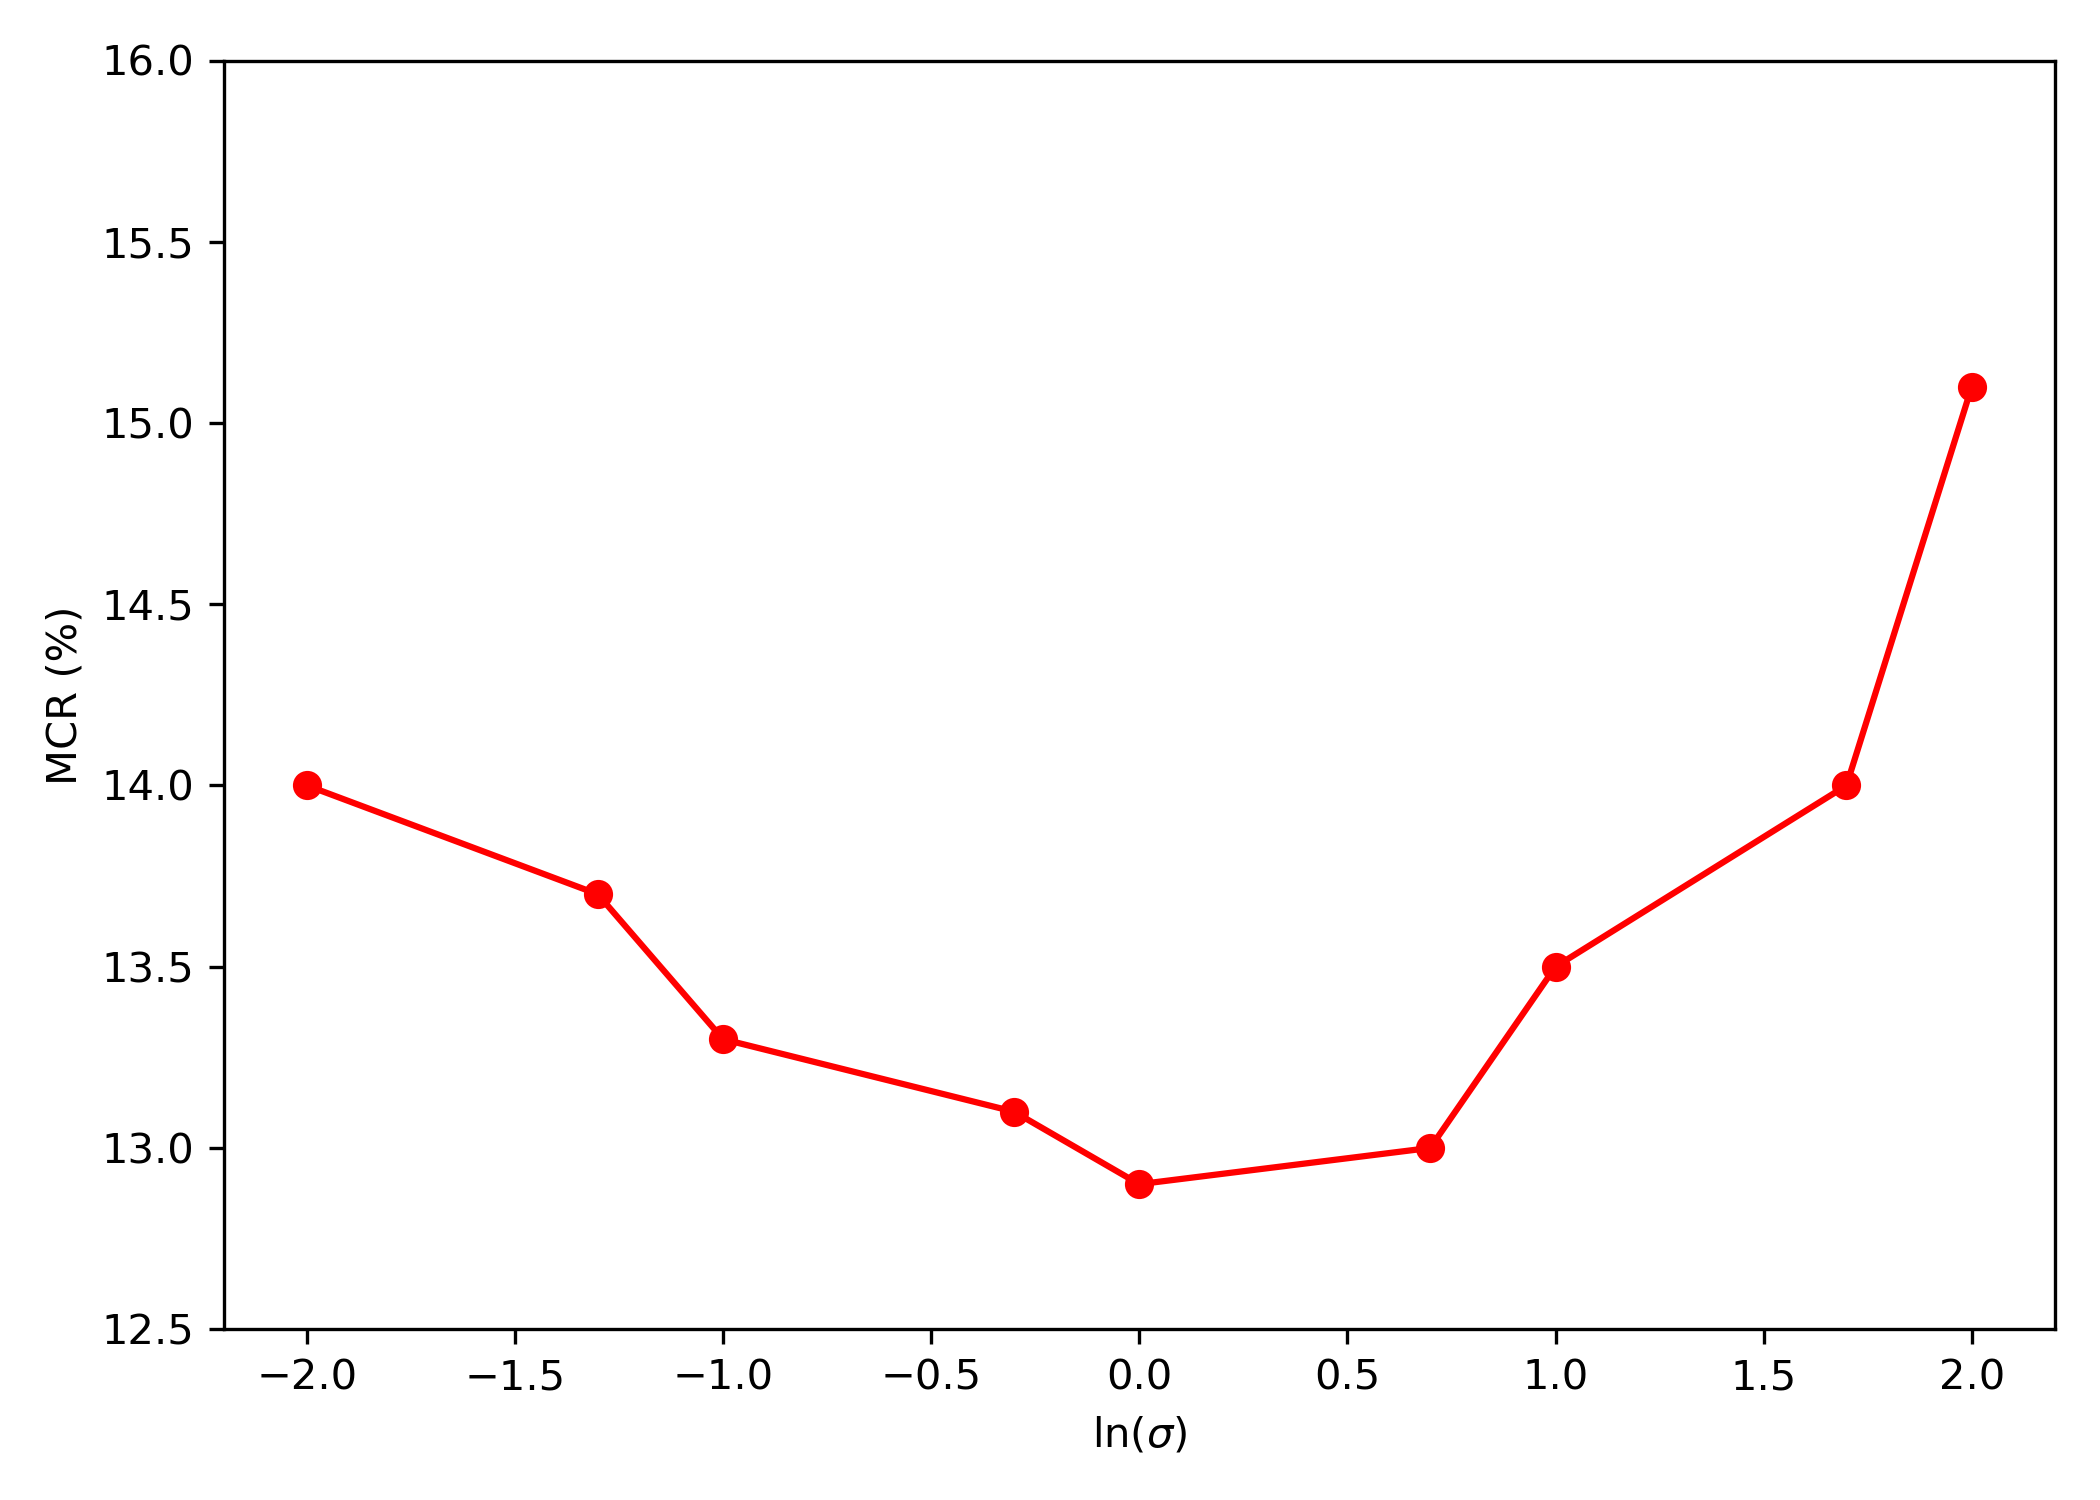
\includegraphics[width=0.7\linewidth]{char2_sigma.png}
    \caption{\label{fig:sigma}在$MultipleGaussian$数据集上,PTR=5\%时dPU算法基于不同比例参数$\sigma$的稳态MCR值。}
\end{figure}

对于锚点数据判定条件式\eqref{Anchor_manifold_condition}中的阈值$\zeta$,若过小会导致锚点数据集过大以至于通信代价过高,
过大则会导致数据集过小全局约束效果不佳。
因此对阈值$\zeta$进行间隔为0.1的搜索,其结果如\autoref{fig:zeta_1}和\autoref{fig:zeta_2}所示。在$\zeta=0.6$时,MCR已基本达到平缓而锚点数据集大小则加速上升。因此,综合考虑性能和通信代价两个方面,
在$MultipleGaussian$数据集上设置阈值$\zeta=0.6$。
后续各真实数据集中使用间隔为0.1的网格搜索在$\left[0,1\right]$中分别搜寻最合适的值。
\begin{figure}
    \centering
    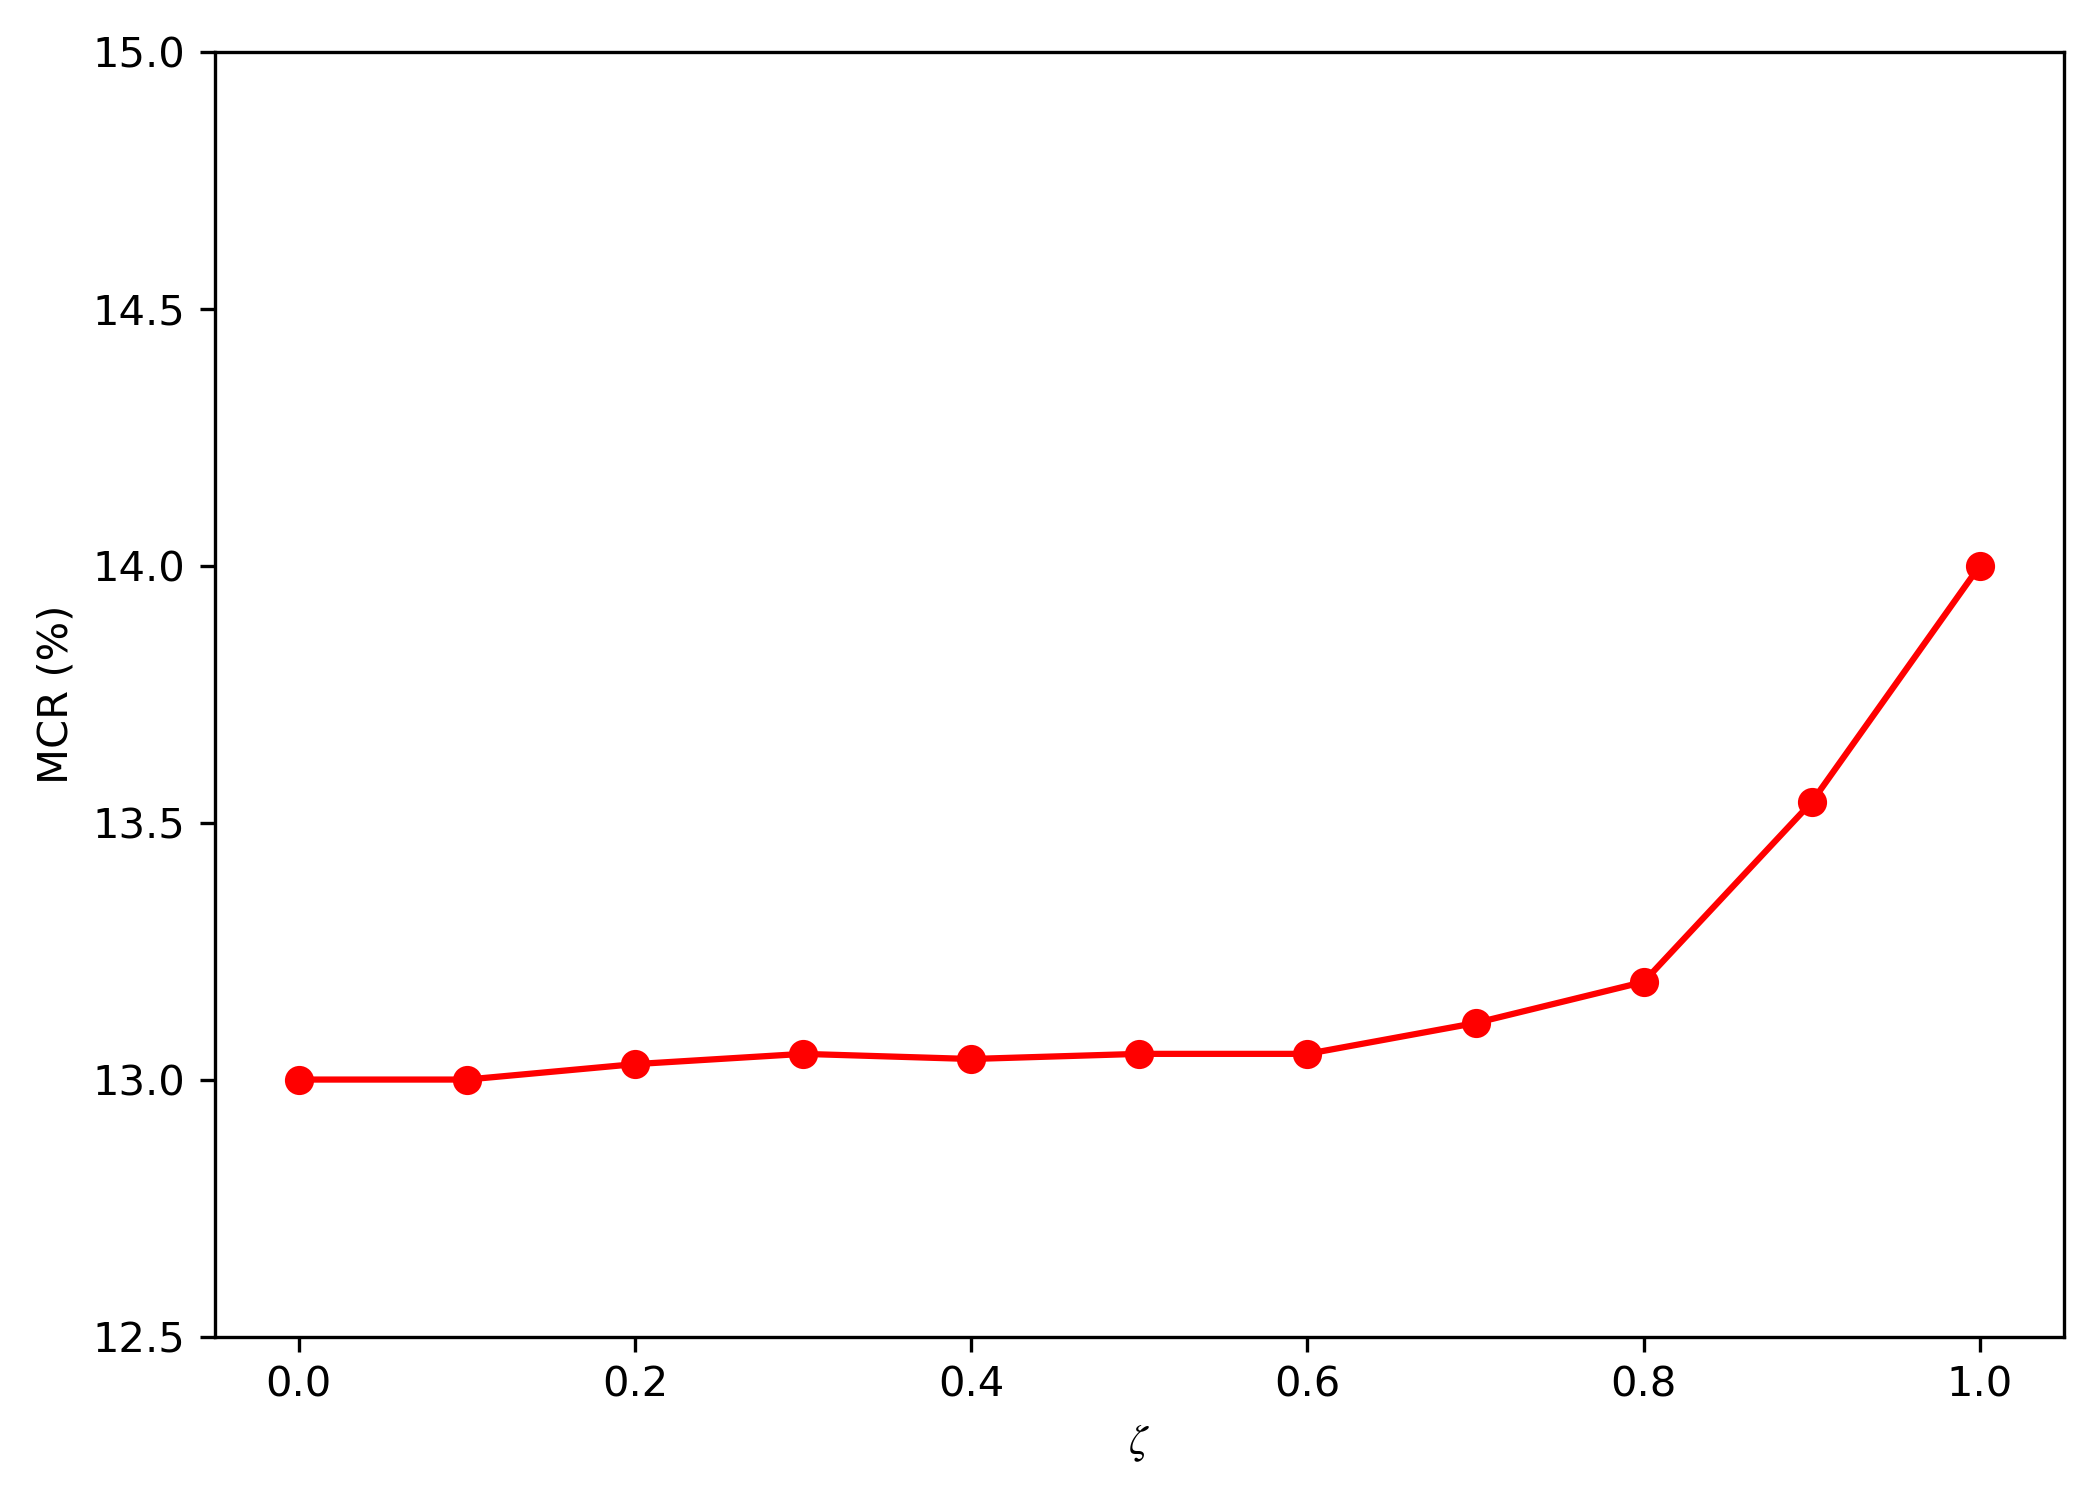
\includegraphics[width=0.7\linewidth]{char2_zeta_1.png}
    \caption{\label{fig:zeta_1}在$MultipleGaussian$数据集上,PTR=5\%时dPU算法基于不同锚点阈值$\zeta$的稳态MCR值。}
\end{figure}
\begin{figure}
    \centering
    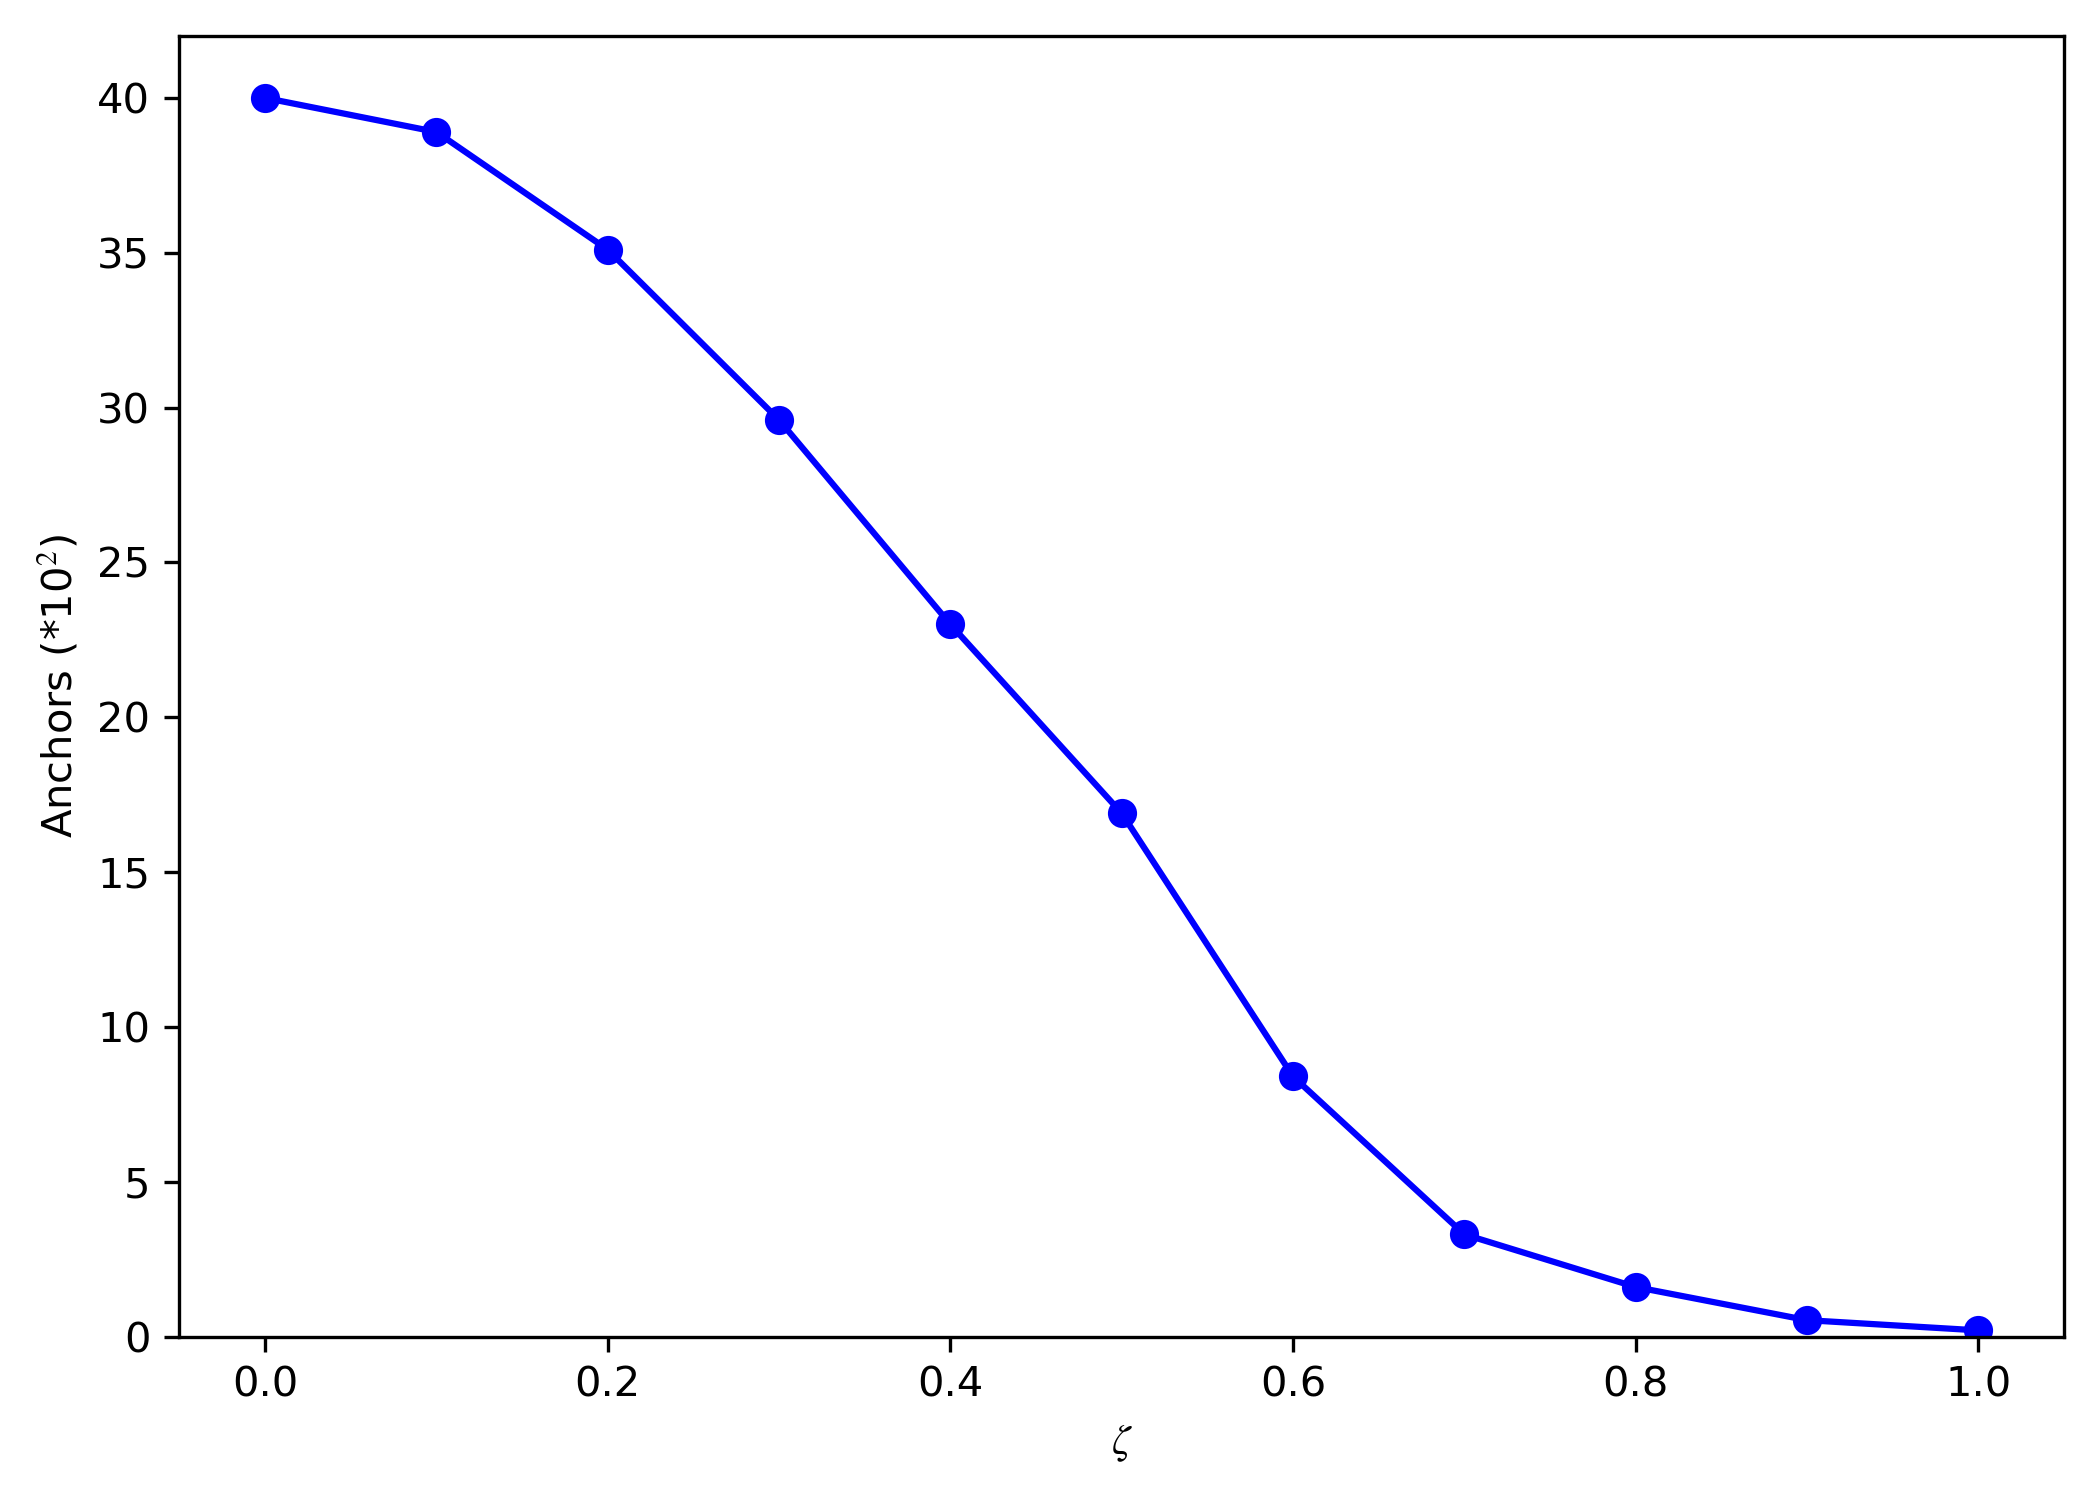
\includegraphics[width=0.7\linewidth]{char2_zeta_2.png}
    \caption{\label{fig:zeta_2}在$MultipleGaussian$数据集上,PTR=5\%时dPU算法基于不同锚点阈值$\zeta$的锚点数据集大小。}
\end{figure}

接下来对影响随机特征映射逼近核函数性能的关键因素,即随机特征映射的映射维度$D$进行探索,并验证可加性核$\chi^2$相比于高斯核Gau的在所需映射维度方面的优势。本文对dPU算法在$MultipleGaussian$数据集上的MCR与可加性核$\chi^2$和高斯核Gau的映射维度$D$的关系进行了数值仿真。其结果如\autoref{fig:D_1}所示,对于可加性核$\chi^2$,$D=25~(S=1)$之后,MCR迅速下降并已达到最佳性能;对于高斯核Gau,需要扩大映射维度到$D=200$时才可逼近最佳性能。而计算所需CPU时间则如\autoref{fig:D_2}所示,随着映射维度$D$的增长而线性上升,因此综合考虑算法性能和计算资源消耗,使用$\chi^2$核的最小映射维度$D=25~(S=1)$就足以逼近最佳非线性性能。
\begin{figure}
    \centering
    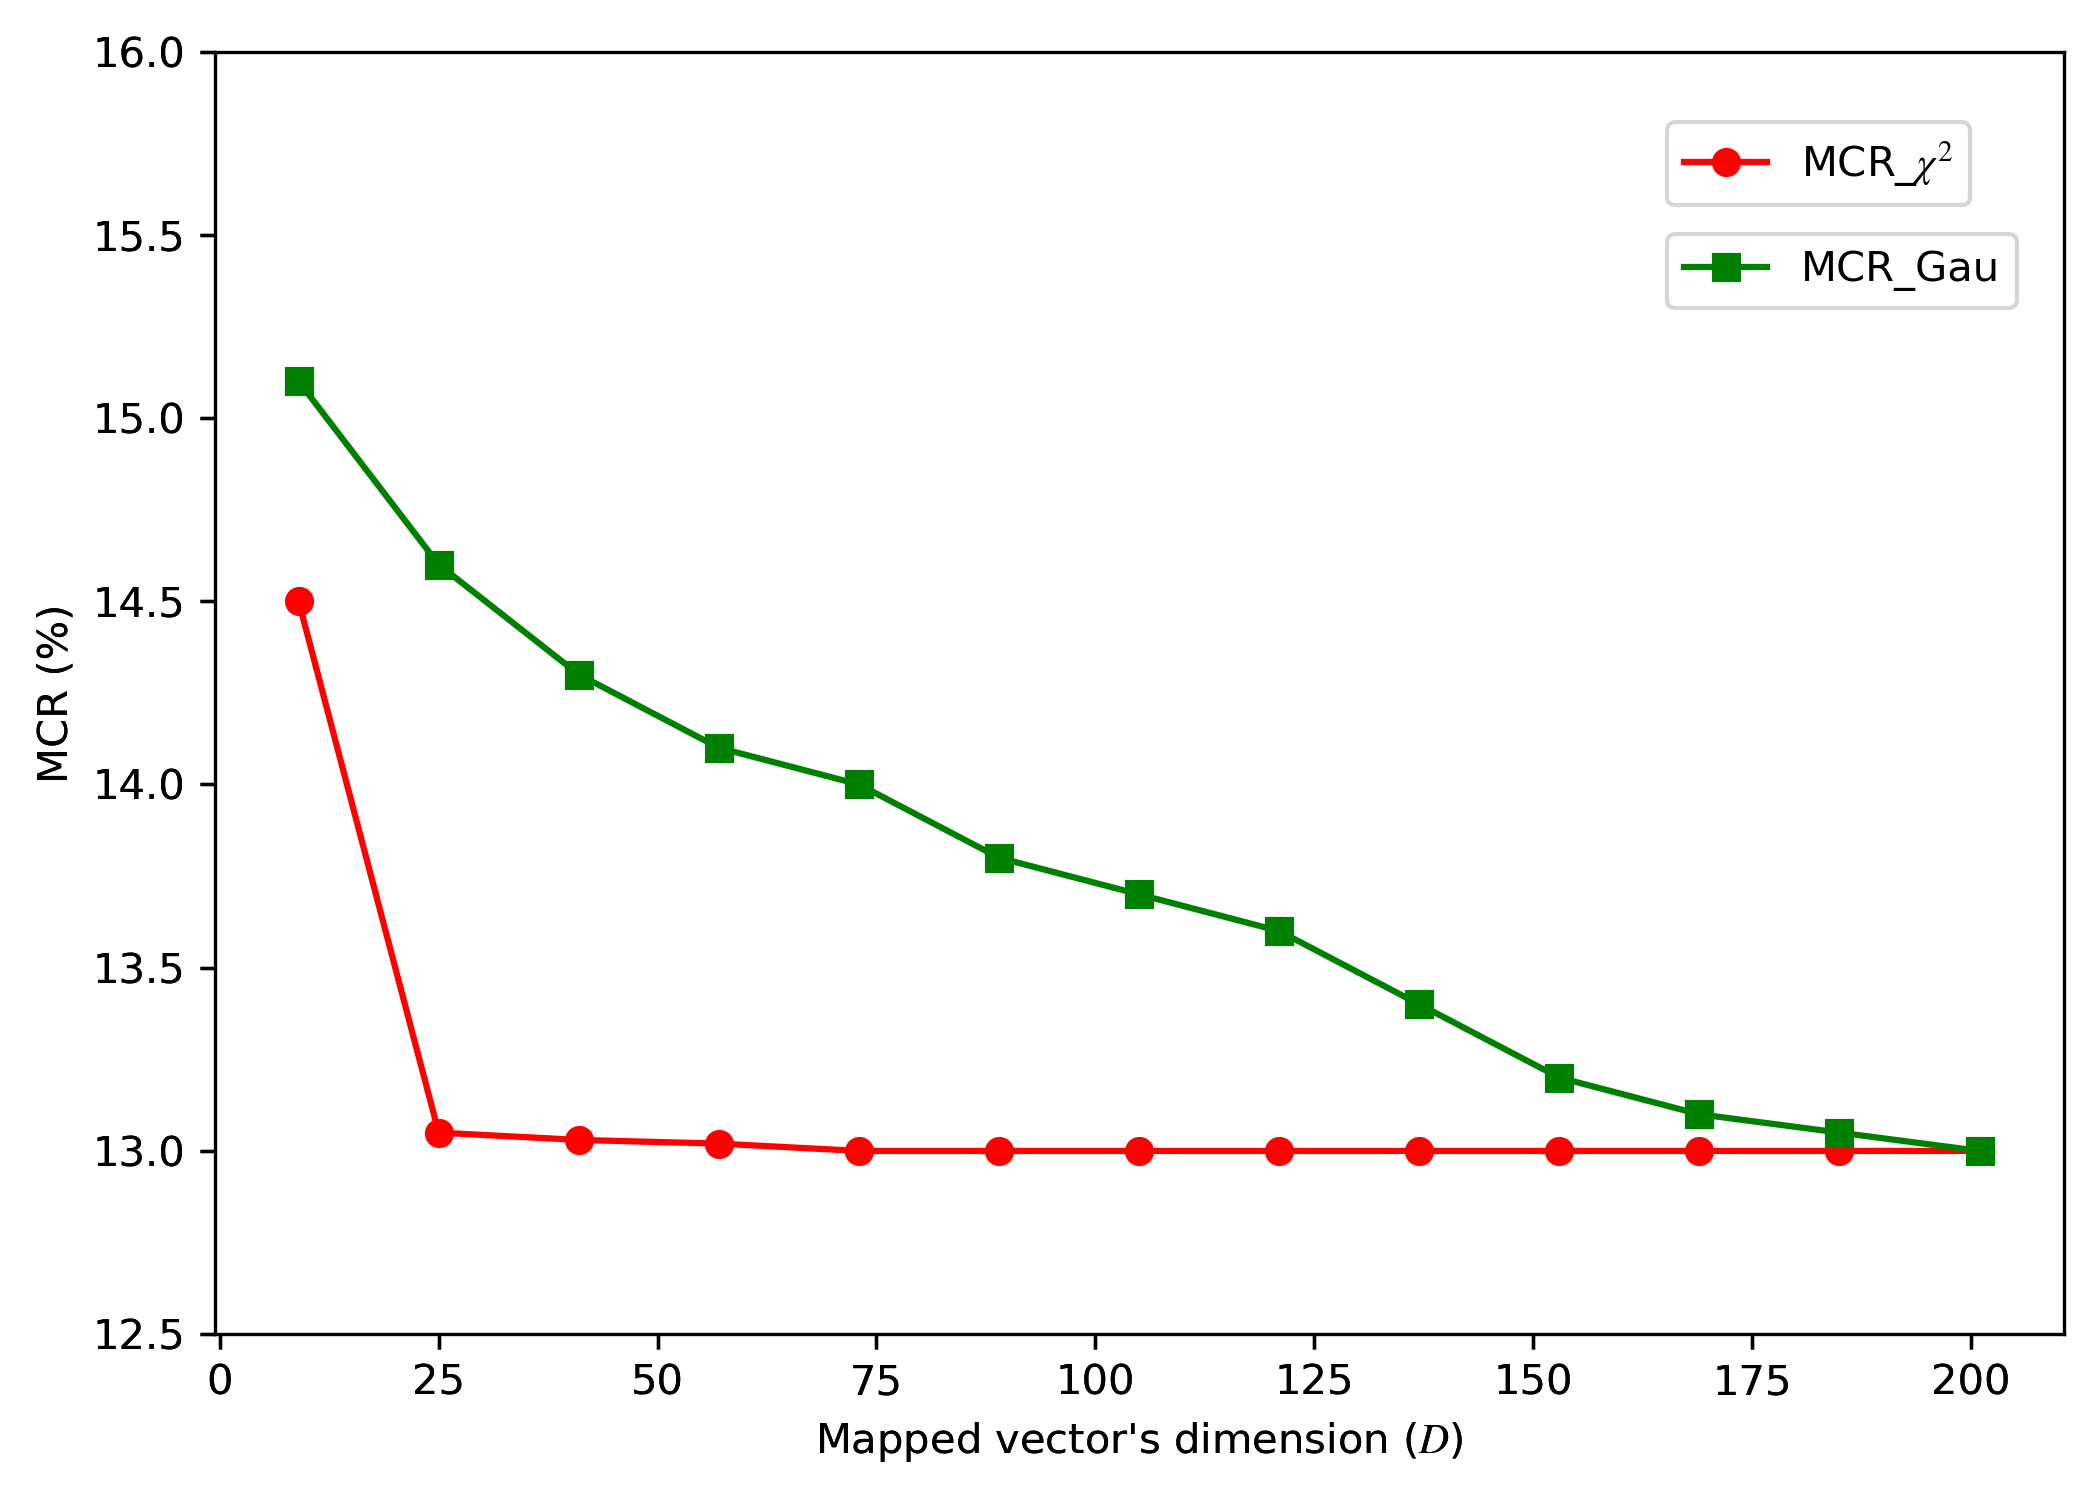
\includegraphics[width=0.7\linewidth]{char2_D_1.png}
    \caption{\label{fig:D_1}在$MultipleGaussian$数据集上,PTR=5\%时基于不同核函数的dPU算法在不同映射维度$D$上的稳态MCR值。}
\end{figure}
\begin{figure}
    \centering
    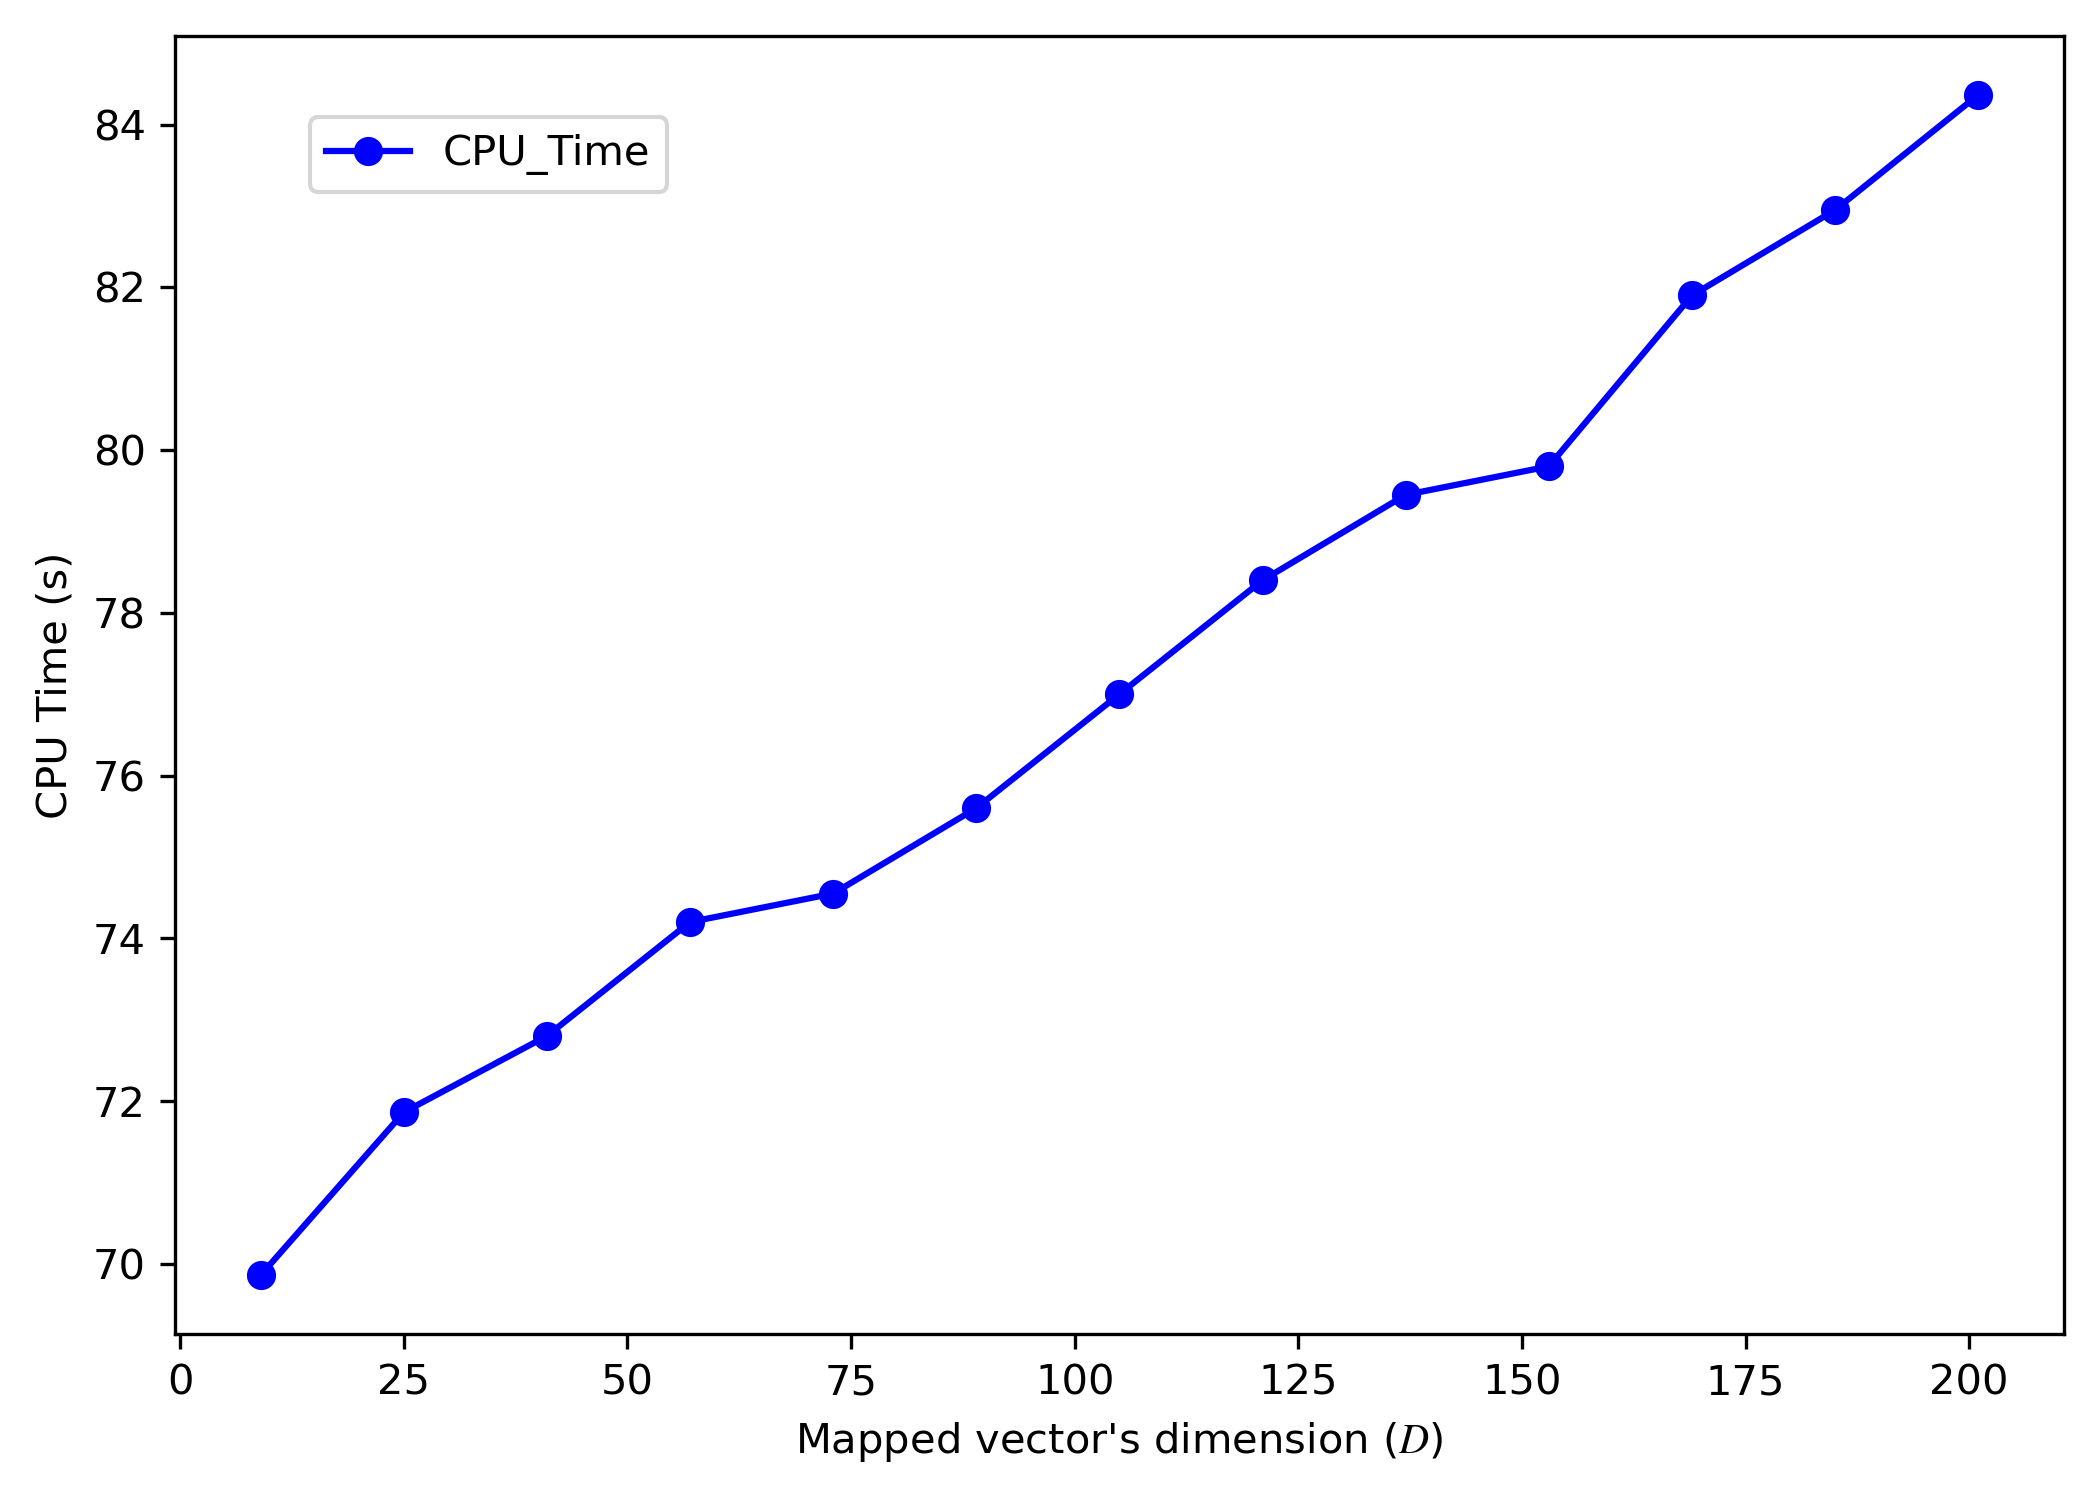
\includegraphics[width=0.7\linewidth]{char2_D_2.png}
    \caption{\label{fig:D_2}在$MultipleGaussian$数据集上,PTR=5\%时dPU算法基于不同映射维度$D$的计算时间。}
\end{figure}

在完成参数设置后,为了进一步研究提出的dPU算法的有效性,本文将其与集中式PU (centralized PU,cPU)和LLSVM算法在不同PTR上的性能进行了比较。
如\autoref{fig:dcL}所示,可以看到在PTR处于$\left[1\%,10\%\right]$, dPU的稳态MCR值相比于LLSVM的稳态MCR值存在着明显的降低,
这意味在标注比例很低的情况下流形约束对于未知数据分类性能的提升有显著作用。
此外,根据\autoref{fig:dcL}中,dPU算法与cPU算法的稳态MCR值对比结果表明,本文所提出的基于锚点数据和ADMM优化方法的分布式算法
在数据存储在不同节点且节点间仅传递少量信息的情况下可以达到较为理想的全局最优性能。
\begin{figure}
    \centering
    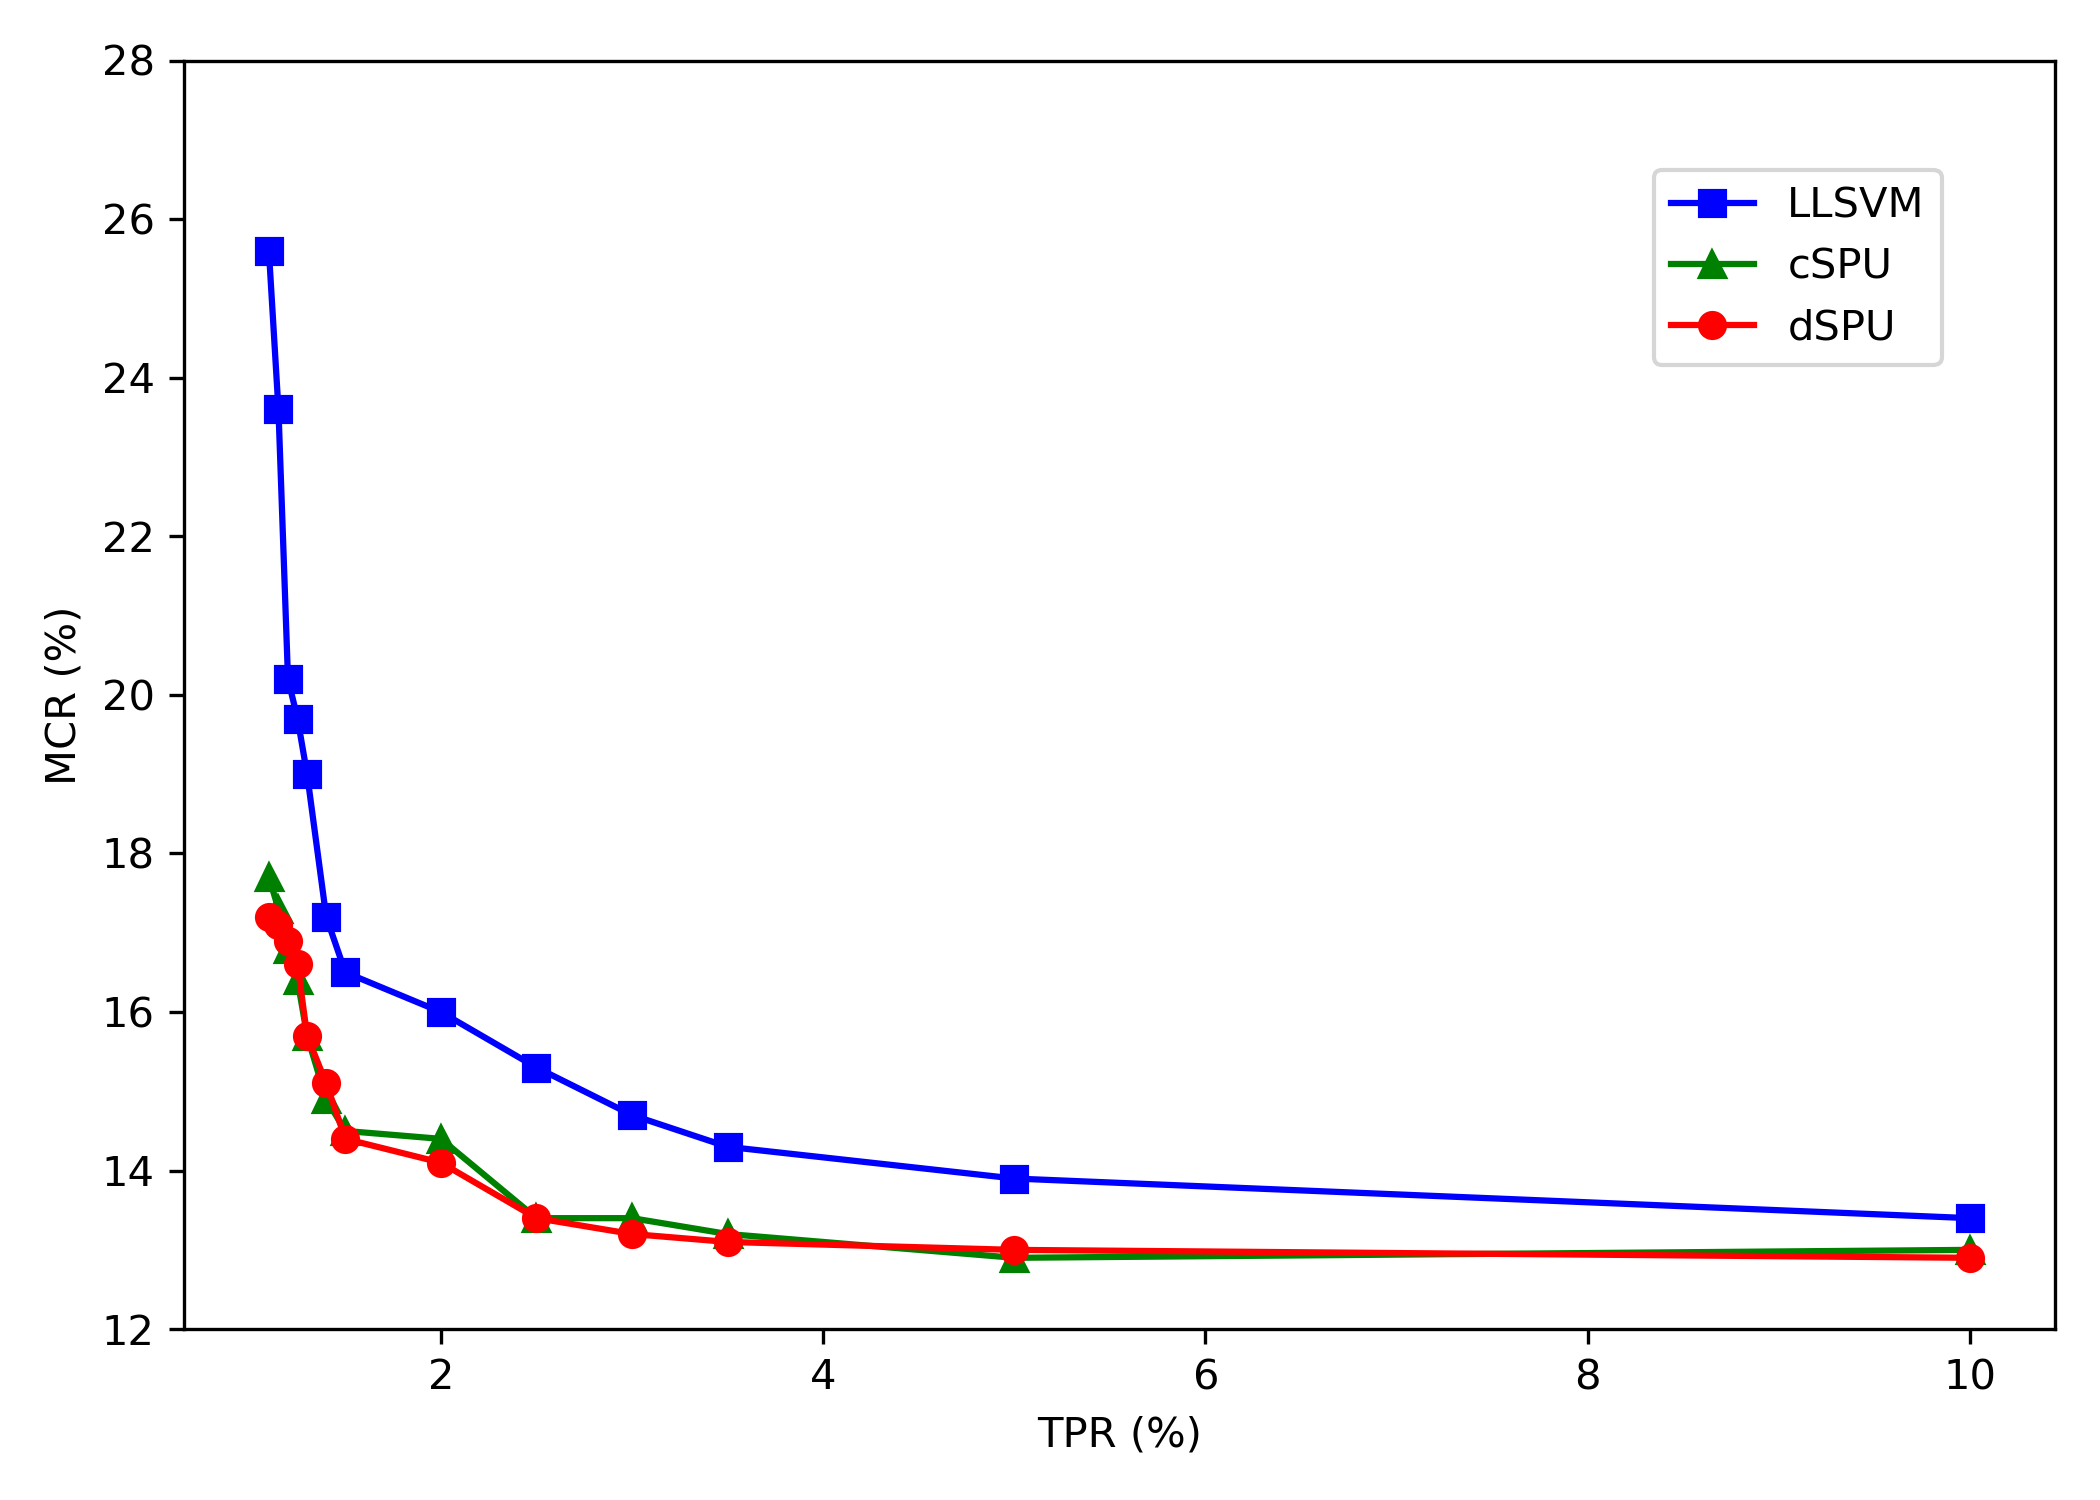
\includegraphics[width=0.7\linewidth]{char2_dcL.png}
    \caption{\label{fig:dcL}在$MultipleGaussian$数据集上,不同PTR条件下不同算法的稳态MCR值。}
\end{figure}

% Chapter
\subsection{真实数据集}
% 详细描述一下数据,如一些分布式场景
\begin{table}[htbp]
    \caption{\label{char2:tab:data_description}数据描述}
    % \begin{tabularx}{\linewidth}{c|c|c|c|c}
    % \begin{tabularx}{\textwidth}{X|X|X|X|X}$
    \begin{tabularx}{\textwidth}{XXXXXX}
        \hline
        数据集  & 正样本数 & 负样本数 & 训练集大小 & 测试集大小 & $\zeta$ \\ \hline
        Fried  & 20341 & 20427 & 32613 & 8155 &  0.6\\
        AirPollution & 1652 & 4905 & 5245 & 1312 &  0.7\\
        HTRU2 & 16258 & 1639 & 14317 & 3580  & 0.4\\
        DUCIN & 3620 & 6380 & 8000 & 2000 &  0.5\\
        Occupancy & 4750 & 15810 & 16448 & 4112 &  0.8\\ \hline
    \end{tabularx}
\end{table}
为了展示dPU算法的优越性能,本文测试了其在各种基准数据集上的MCR性能,其中包括来自OpenML\cite{OpenML}的$AirPollution$数据集(其由房间中各传感器搜集到的CO、SO$_2$浓度等数值组成)和$Fried$数据集(由Friedman和Breiman所构建的用于回归任务的数据集);
以及来自UCI \cite{UCI}的$HTRu2$数据集(使用各地的天文观测站搜集到的电波特征判断是否脉冲星),$DUCIN$数据集(将UCI中的数据进行整理归类得到)和$Occupncy$数据集(根据房间中传感器探测到的湿度、光照和CO$_2$等信息判断是否住人)。
上述各数据集的样本总数从6558到40769不等,样本的属性数从3到13不等,详细描述见\autoref{char2:tab:data_description}
其中划分后的训练集和测试集中的正负类比例与原数据集相同。
对阈值$\zeta$在不同数据集上进行范围为$\left[0,1\right]$间隔为0.1的网格搜索并将最优结果展示于
\autoref{char2:tab:data_description}中,核函数将使用$\chi^2$核并将核映射维度设置为$D=25~(S=1)$。

\begin{table}[htbp]
    \caption{\label{char2:tab:MCRs}不同算法在真实数据集上的性能(MCR)比较}
    % \begin{tabularx}{\linewidth}{c|c|c|c|c}
    % \begin{tabularx}{\textwidth}{X|X|X|X|X}
    \begin{tabularx}{\textwidth}{XXXXXXX}
        \hline
        \multirow{2}*{数据集} & \multirow{2}*{PTR(\%)} & \multicolumn{5}{c}{MCR(\%)}\\
        \cline{3-7}
        \multicolumn{1}{c}{} & & WLR & SMD  & PMPU & LLSVM & dPU\\
        \hline
        \multirow{3}*{Fried} 
        & 3.0 & 23.2$\pm$0.2 & 26.4$\pm$0.1 & 17.5$\pm$0.5 & 18.5$\pm$0.9 & \textbf{14.6$\pm$2.0} \\
        & 6.0 & 22.0$\pm$0.1 & 25.9$\pm$0.0 & 18.0$\pm$0.1 & 16.6$\pm$0.8 & \textbf{12.5$\pm$0.9} \\
        & 10.0 & 22.5$\pm$0.1 & 25.5$\pm$0.1 & 19.2$\pm$0.3 & 16.2$\pm$1.2 & \textbf{12.0$\pm$1.1} \\ \hline

        \multirow{3}*{AirPollution} 
        & 3.0 & 14.8$\pm$0.1 & 25.2$\pm$0.2 & \textbf{9.2$\pm$0.4} & 10.9$\pm$0.9 & 13.7$\pm$0.9 \\
        & 6.0 & 12.9$\pm$0.4 & 25.2$\pm$0.2 & 8.5$\pm$0.2 & 7.8$\pm$0.4 & \textbf{7.1$\pm$}1.0 \\
        & 10.0 & 11.1$\pm$0.2 & 23.6$\pm$0.3 & 9.5$\pm$0.3 & 6.5$\pm$0.8 & \textbf{3.0$\pm$}0.3 \\        \hline
        
        \multirow{3}*{HTRu2} 
        & 3.0 & $\backslash$ & 21.7$\pm$0.1 & 4.2$\pm$1.5 & $\backslash$ & \textbf{4.0$\pm$0.5} \\
        & 6.0 & $\backslash$ & 20.1$\pm$0.0 & \textbf{2.9$\pm$0.5} & $\backslash$ & 3.0$\pm$0.3 \\
        & 10.0 & $\backslash$ & 17.0$\pm$0.3 & 2.7$\pm$0.6 & $\backslash$ & \textbf{2.5$\pm$0.4} \\        \hline
        
        \multirow{3}*{DUCIN} 
        & 3.0 & 25.7$\pm$0.2 & 32.7$\pm$0.3 & \textbf{19.8$\pm$0.1} & 27.5$\pm$1.0 & 21.2$\pm$0.8 \\
        & 6.0 & 23.0$\pm$0.2 & 28.1$\pm$0.5 & 20.6$\pm$0.5 & 19.0$\pm$1.1 & \textbf{15.1$\pm$0.3} \\
        & 10.0 & 22.4$\pm$0.4 & 28.4$\pm$0.3 & 19.0$\pm$0.2 & 17.6$\pm$1.5 & \textbf{13.5$\pm$0.4} \\        \hline
        
        \multirow{3}*{Occupancy} 
        & 3.0 & $\backslash$ & 12.1$\pm$0.3 & 5.8$\pm$2.1 & 9.6$\pm$2.2 & \textbf{4.3$\pm$1.0} \\
        & 6.0 & $\backslash$ & 12.2$\pm$0.1 & 3.9$\pm$1.0 & 5.6$\pm$0.9 & \textbf{3.0$\pm$1.0} \\
        & 10.0 & $\backslash$ & 12.5$\pm$0.3 & 5.3$\pm$1.2 & 3.9$\pm$0.9 & \textbf{0.5$\pm$0.2} \\        \hline
        
        平均排名 & & 4.40 & 4.60 & 2.40 & 2.50 & \textbf{1.27}\\        \hline
    \end{tabularx}
\end{table}
在以上参数设置下,对本文所提出的dPU算法基于不同PTR的性能进行了测试。
并且为了性能比较,在\autoref{char2:tab:MCRs}中也将一起给出一些PU学习算法的结果,
其中包括结合基于观测偏差的负例选择法和蒙特卡罗概率逼近(selection of negatives through observed
bias combined with monte carlo probability approximation,SM)的两步法\cite{Youngs_SMD_2015},
基于标签噪声的加权Logistic回归算法(label noise PU learning algorithm weighted logistic regression,WLR) \cite{Lee_WLR_2003},
以及基于正向间隙的PU学习算法(psositive margin based PU learning,PMPU)\cite{Gong_Margin_2018}和大间隙标签校准支持向量机
(large-margin label-calibrated support vector machine,LLSVM)\cite{Gong_LLSVM_2019}。
在\autoref{char2:tab:MCRs}中,“$\setminus$”表示该算法在当前条件下不收敛,粗体则表示该条件下获得最优的性能的算法,
“$\pm$”前后为该条件下50次仿真结果的平均值和标准差。
如\autoref{char2:tab:MCRs}所示,dPU算法在不同PTR情况下的分类性能多数都优于其他算法,说明其在实际应用中具有普遍的优越性。
如最后一行平均排名所示,dPU算法在这些算法中排名第一,这意味着它在PU数据分类方面是优于其他算法的。

% Chapter 2.5
\section{本章小结}\label{Summary}
本节针对正例数据和无标记数据分布于不同节点的学习场景,提出了一种分布式正例无标注学习算法。
本文引入随机特征映射以实现分布式条件下不需要原始数据传输也可以计算核函数的技巧来实现复杂非线性分类,设计代价函数时提出了自适应的门限来约束未标注数据分布情况,并引入了基于锚点数据的流形正则化使本地流形约束逼近全局流形约束性能,从而有效地利用了大量未标记数据中的底层信息。
在分布式场景下,利用各节点的损失函数构造了去中心化的全局优化问题,采用交替乘子法仅通过从邻居节点传来的少量信息使各节点协同解决全局优化问题以得到全局最优的分类器。对算法的收敛性和计算复杂度进行了分析。
此外,本文对模拟数据集进行探索确定了最优参数设置,并最终在真实数据集上结合其余PU学习算法进行了仿真。实验结果表明,本文提出的dPU算法在没有负例训练数据且正例标注比例极小的情况下,也能学到良好的分类效果,并且具有相比于其他同类算法更优越的分类性能。


% 我改到这了
% Chapter 3
\chapter{分布式单正例无标注多标签学习}
\section{引言}
在上节我们讨论了基于单标签的正例无标注学习算法,但在实际任务中一个数据可能存在多种标签,
如在目标检测中一张图片通常会出现多个目标、文本情感分析中一段文本也将会有多种情感标签等\cite{Zhang_MultiLabel_2018}。
以一张图片为例,它可能会有多个标签类别,但通常要完全标注所有类标签的正负(即属于该类与否)是困难的。例如,在\autoref{Char1:fig:multi-label1}中,飞机类最容易被标注,房屋类和树类次之,而草类和指示牌类则很难
被关注到。这种标签分布情况极其常见,以至于在繁重的标注任务中,标注人员会仅对正向标注部分甚至仅对最明显的某个标签类感兴趣,如对\autoref{Char1:fig:multi-label1}中的飞机类进行正向标注\cite{Van_Inaturalist_2018}。
若在仅有单个标签标注的情况下,也可以学到多标签分类信息,那么繁琐的多标签标注任务就变成较为简单的单个正例标注任务,从而
{大大降低了人力标注的成本。}
因此,本节将考虑多标签学习领域中最极端的情况,即在多个标签中只有部分数据的一个标签被明确标注为正,其余标签都为未标注状态的
单正例多标签(single positive multi-label,SPM)数据。此外,进一步考虑除了SPM 数据之外,仍包含相当比
例无任何标签被标注的单正例无标注多标签(single positive and unlabeled multi-label,SPUM)数据。
\begin{figure}[htbp]
    \centering
    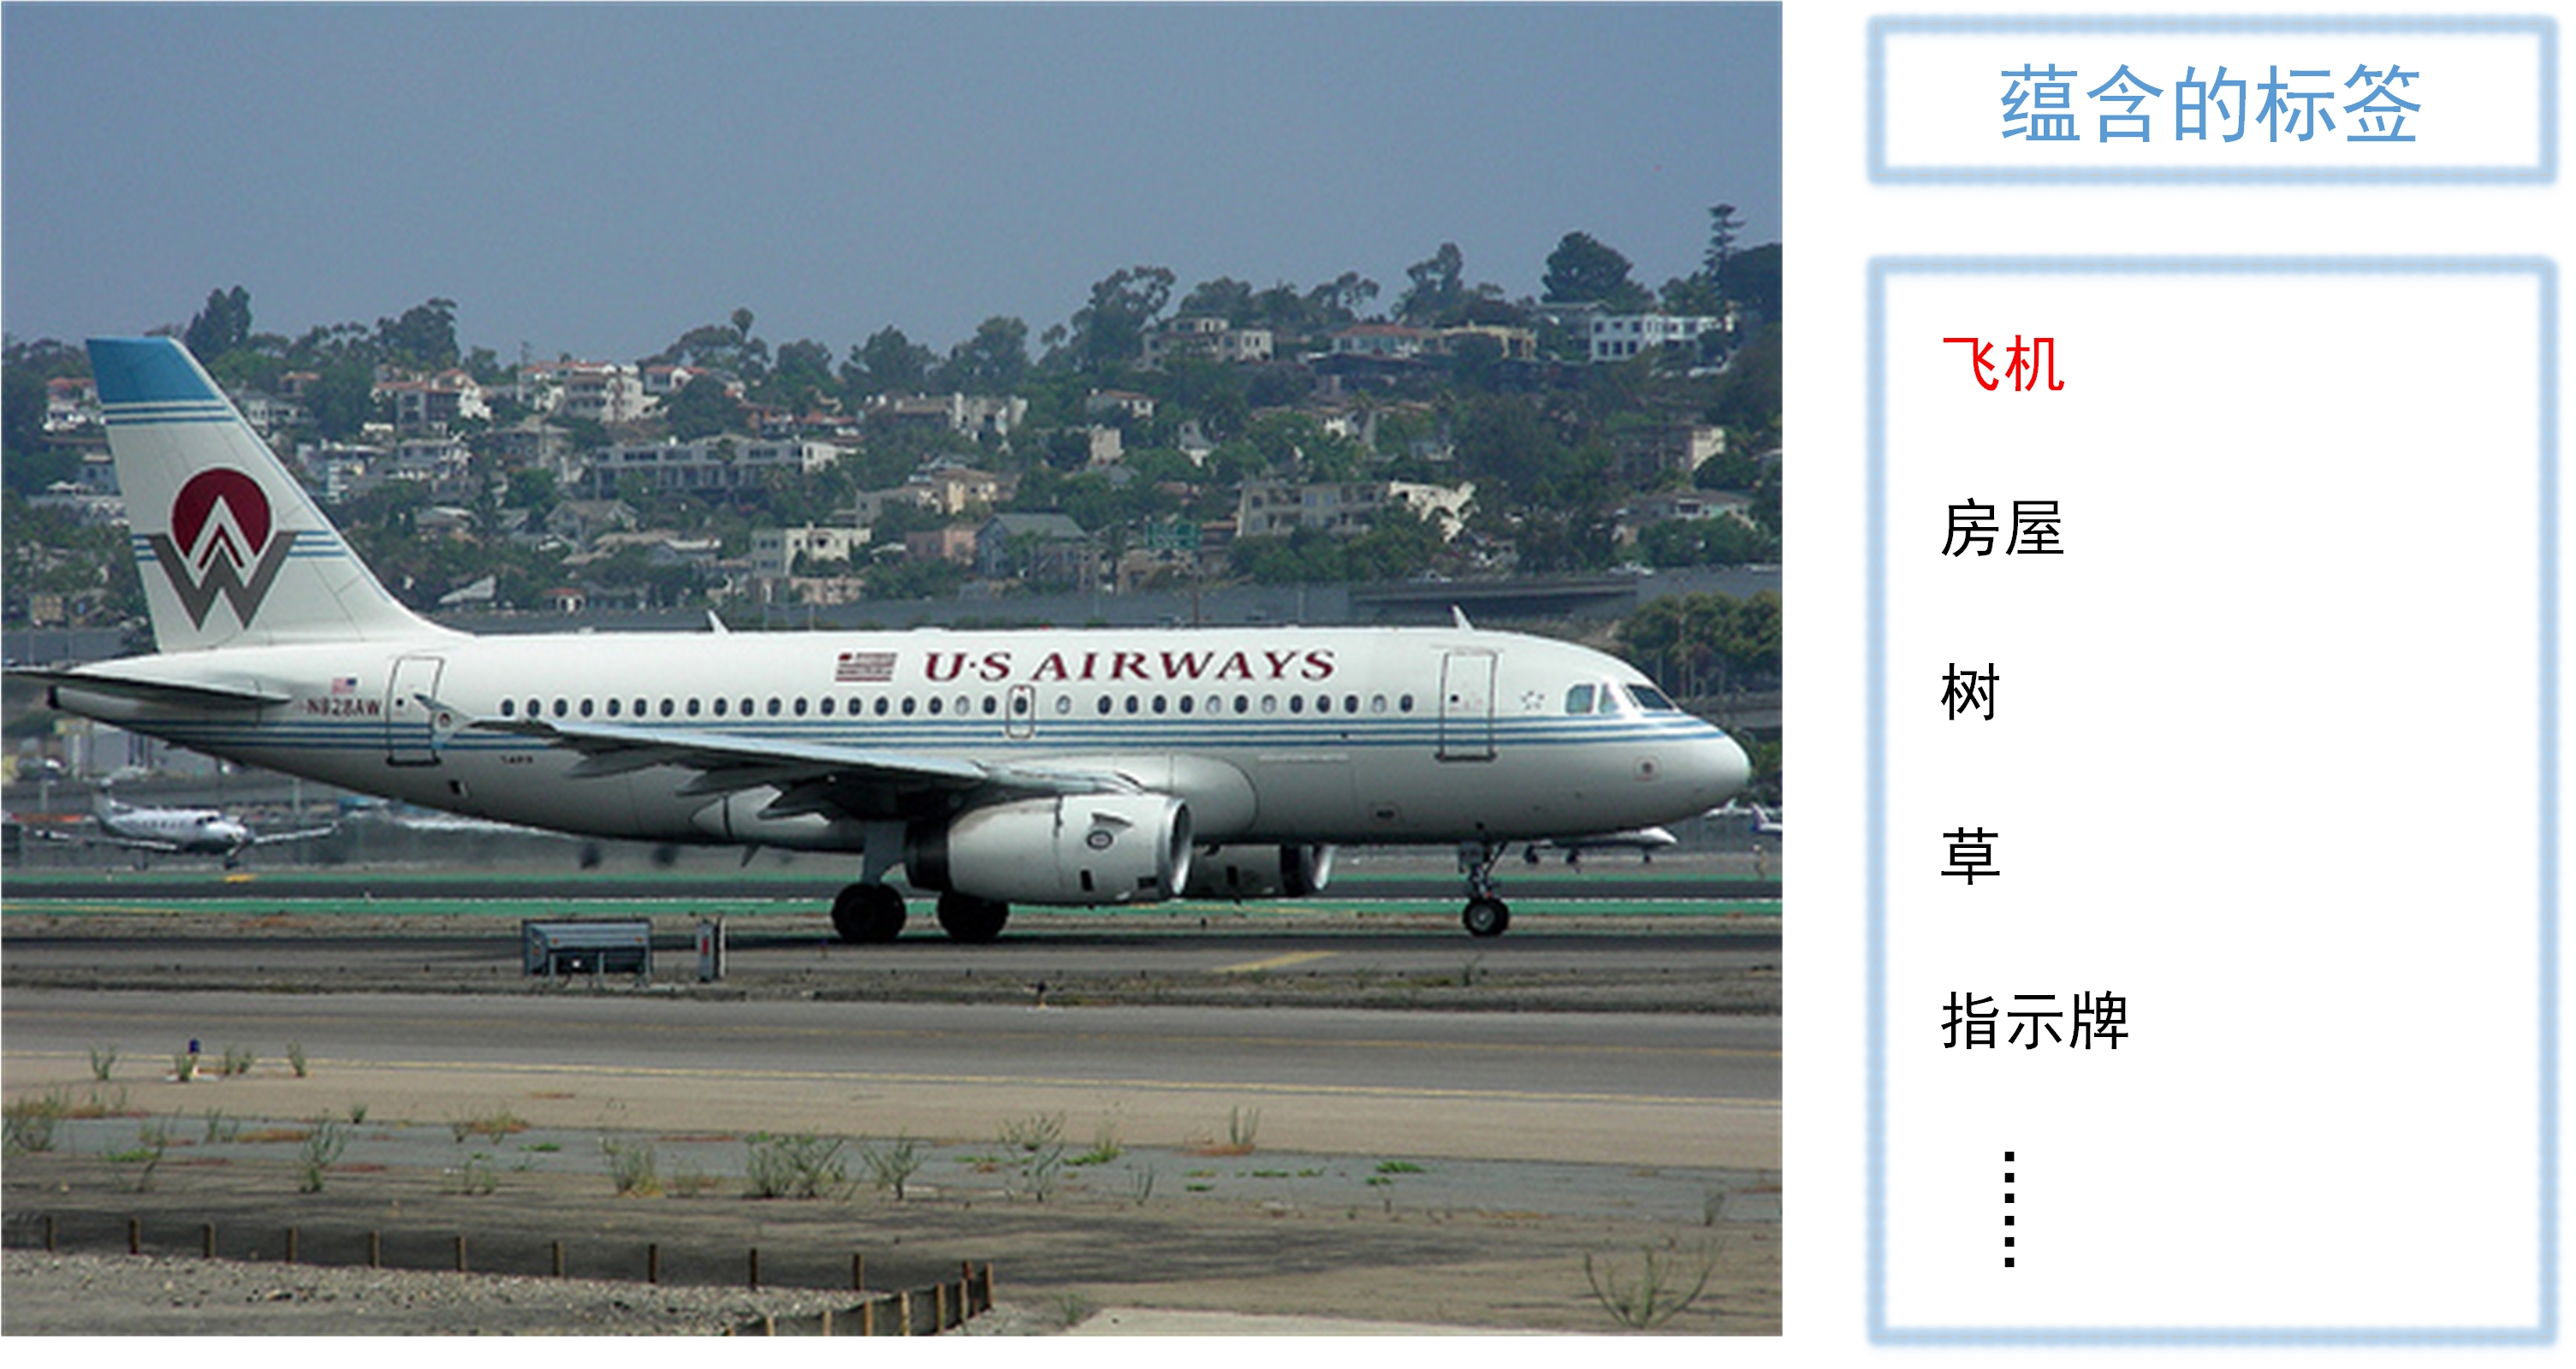
\includegraphics[width=0.7\linewidth]{Char1/部分标签图1.jpg}
    \caption{\label{Char1:fig:multi-label1}一个多标签数据的例子。}
\end{figure}

在本章中,我们考虑在各分布式节点中仅有部分数据的单个正例标签被标注的多标签学习场景,提出了基于SPUM数据的分布式学习算法。本章剩余部分的简介如下:
在\ref{Char3_Preliminaries}节,简单地进行了问题描述。
在\ref{Char3_LossDesign}节,提出两种适用于分布式节点中SPUM数据的去中心化损失函数,并提出了全局优化问题。
在\ref{Char3_Distributed}节,对全局优化问题使用分布式梯度下降法进行优化并对收敛性进行了分析,
然后引入事件触发机制以减少节点间通信量。
在\ref{Char3_Experiments}节,利用若干数据集对提出的算法进行了测试,并通过与其他算法的对比以及统计测试证实了所提方法的优越性。
\ref{Char3_Summary}节,对本章的工作做出了总结。

% Chapter 3.1
\section{问题描述}\label{Char3_Preliminaries}
{如上文所述,本章探讨一个由$J$个节点组成的分布式网络,其中每个节点都包含一定的SPUM数据。}
该网络可以用一个无向图$\mathcal{G}=\left\{\mathcal{J},\mathcal{B}\right\}$来表示,
其中$\mathcal{J}=\left\{1,2,...,J\right\}$表示节点集,$\mathcal{B}=\left\{\mathcal{B}_j\right\},j\in\mathcal{J}$
表示各节点的邻居节点的编号集,$\mathcal{E}=\left\{\left(j,b\right)\right\},j\in\mathcal{J},b\in\mathcal{B}_j$表示节点$j$与邻居节点的边集。各分布式节点各自所分配的多标签数据集为$\mathcal{N}_j=\left\{1,2,...,N_j\right\}$,
其中每个数据$\boldsymbol x_n,n\in\mathcal{N}_j$都有$L$个标签并将标签集记为$\mathcal{L}=\left\{1,2,...,L\right\}$。
在各节点的数据集$\mathcal{N}_j$中,除了有部分已标注单个正例标签的SPM数据集$\mathcal{N}_j^l=\left\{1,2,...,N_j^l\right\}$之外,
仍然存在相当比例的未进行任何标注的数据集$\mathcal{N}_j^{ul}=\left\{N_j^{l}+1,N_j^{l}+2,...,N_j^l+N_j^{ul}\right\}$。

在单正例多标签数据集$\mathcal{N}_j^l$中,每个数据的$L$维标签向量仅有一个标签被标注到,本文使用观测向量$\boldsymbol z_n$表示这种被不完全标注的标签向量,则单正例多标签数据$\left(\boldsymbol x_n, \boldsymbol z_n\right), n \in \mathcal{N}$的可被描述为:
\begin{equation}
    \begin{split}
        & z_{n i} \in\{1, \varnothing\} \text { for all } n \in \mathcal{N}_j^l, i \in \mathcal{L}, \\
        & \sum_{i \in \mathcal{L}} \mathbb{I}_{\left[z_{n i}=1\right]}=1 \text { for all } n \in \mathcal{N}_j^l,
    \end{split}
\end{equation}
其中$\varnothing$为未知标签(其可能为1或0)。
{而未进行任何标注的数据集$\mathcal{N}_j^{ul}$中每个数据的$L$维标签向量都只有未知标签$\varnothing$
,即$z_{n i}=\varnothing~\text{for all}~n\in\mathcal{N}_j^{ul},i\in\mathcal{L}$。}

定义$\boldsymbol f\left(\boldsymbol\theta_j,\boldsymbol x_n\right)$为分类器模型的输出,其中$\boldsymbol x_n$为单个数据,
$\boldsymbol\theta_j$代表节点$j$的模型参数。
为了算法表示的简洁性,本文将在下文中使用$\boldsymbol f_n$代表$\boldsymbol f\left(\boldsymbol\theta_j,\boldsymbol x_n\right)$,
并用$f_{ni},i\in\mathcal{L}$代表$\boldsymbol f_n$中的每一个输出标签值。
多标签学习常见于目标检测领域,用以检测一张图片中可能出现的多种物体。因此本文使用目标检测算法常用的ResNet50
作为基本框架对图片进行特征提取,并在特征参数层使用上述各种损失函数。
如\autoref{fig3:arc1},在一张图片经过预训练好的特征提取器ResNet50之后得到特征向量,此后根据参数$\boldsymbol \theta_j$经过计算得到输出向量$\boldsymbol f_n$,{将其和观测向量$\boldsymbol z_n$送入损失函数后通过梯度回传优化参数。
如何在各节点仅交换少量信息的条件下,通过各节点的梯度以及信息传递使各节点最终得到一致的全局最优解$\boldsymbol\theta^*$是本章算法的主要目标。}
\begin{figure}
    \centering
    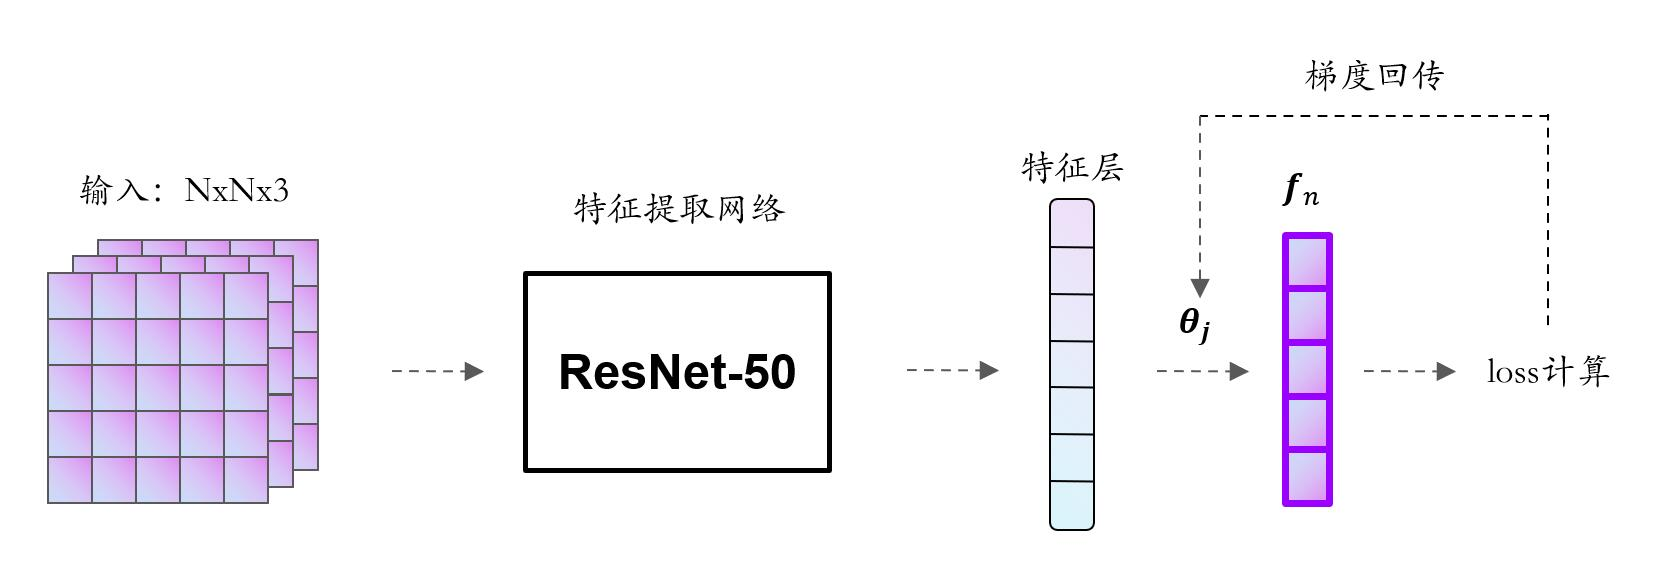
\includegraphics[width=1\linewidth]{char3_arc1_base.jpg}
    \caption{\label{fig3:arc1}{使用ResNet作为特征提取网络的损失函数计算框架。}}
\end{figure}

% 我自己看到这了

% Chapter 3.2
\section{基于单正例无标注多标签数据的半监督学习}\label{Char3_LossDesign}
对于完全标注的多标签数据$\boldsymbol x_n,n\in\mathcal{N}_j^{ul}$来说,其标签向量是一个被完整标注的$L$维的标签向量并记为$\boldsymbol y_n$,其中$y_{ni} \in \left\{0,1\right\}, i \in \mathcal{L}$。
完全标注的多标签分类任务可理解为多个二分类任务,将二元交叉熵(binary cross-entropy, BCE)拓展到多标签领域得到最常使用的多标签分类损失函数\cite{Durand_EPR_2019, Nam_BCE_2014},其公式如下:
\begin{equation}
    \label{BCE}
    l_{\mathrm{BCE}}\left(\boldsymbol{f}_{n}, \boldsymbol{y}_{n}\right)= 
    - \frac{1}{L} \sum_{i \in \mathcal{L}}\left[ \mathbb{I}_{\left[y_{ni}=1\right]} \log \left({f}_{n i}\right)
    +\mathbb{I}_{\left[y_{ni}=0\right]} \log \left(1-{f}_{n i}\right)\right],
\end{equation}
其中$\mathbb{I}_{Q}$表示相应条件$Q$下(如$y_{ni}=1$)数值为1。

而对于单正例多标签数据,由于负例标签的缺失即不存在$\mathbb{I}_{\left[y_{ni}=0\right]}$,
会导致损失函数中$\log \left(1-f_{n i}\right)$部分的缺失,从而使模型退化为仅能预测正向的结果。
最直观的一种解决思路是将观测标签为$\varnothing$的部分视为负,{这种“假负”(“assume negative”, AN)损失函数可表示为:}
\begin{equation}
    \label{AN}
    l_{\mathrm{AN}}\left(\boldsymbol{f}_{n}, \boldsymbol{z}_{n}\right) 
    =-\frac{1}{L} \sum_{i \in \mathcal{L}}\left[\mathbb{I}_{\left[\boldsymbol z_{n i}=1\right]} \log \left(f_{n i}\right)
    +\mathbb{I}_{\left[\boldsymbol z_{n i} = \varnothing \right]} \log \left(1-f_{n i}\right)\right].
\end{equation}
这被认为是一种基于噪声的处理方式,其缺点便是在计算$l_{\mathrm{AN}}$时会引入一些错误的负标签即“假负”标签。
{虽然在多标签任务中正标签数量一般远小于负标签数量},此项引入的“假负”标签造成的影响较小,但仍不足以忽略。

{此外,上述$l_{\mathrm{BCE}}$和$l_{\mathrm{AN}}$损失函数只适用于已标注的单正例多标签数据集$\mathcal{N}_j^l$。
但在实际场景中,除了标注数据之外还会存在许多未进行任何标注的数据集$\mathcal{N}_j^{ul}$。
这部分数据一般数量比较庞大,但无法直接采用诸如式\eqref{BCE}或式\eqref{AN}这样的损失函数进行训练,从而无法有效地利用隐藏在这些庞大数据资源背后的潜在信息。基于上述考虑,本节将对上述$l_{\mathrm{BCE}}$和$l_{\mathrm{AN}}$损失函数进行改进,提出一些尽可能保持损失函数简洁的情况下,减少“假负”标签对整体的有害影响,并适用于SPUM数据集的损失函数。}

% Chapter 3.2.1
\subsection{标签平滑}\label{Chapter:LS}
对于使用交叉熵损失函数的多分类任务来说,标签平滑(label smoothing,LS)是一项常用的减少过拟合的优化方式,
它可以避免网络过于自信,从而减少标签噪声的负面影响并增强对未见数据的分类性能\cite{Muller_LS_2019, Szegedy_LabelSmooth_2016}。
既然$l_{\mathbf{AN}}$可视为带有“假负”标签噪声的$l_{\mathbf{AN}}$,
那么尝试引入标签平滑并探索是否有效是一种非常自然的想法。
标签平滑是通过将真实标签$\boldsymbol{y}_n$替换为$\left(1-\epsilon\right)\boldsymbol{y}_n+\epsilon\left(1-\boldsymbol{y}_n\right)$
以实现标注标签从$\left\{0,1\right\}$到$\left[0,1\right]$的一个平滑过渡,其能对错误标签所造成的不良影响起到一定的缓冲作用。
将其应用于“假负”损失函数式\eqref{AN},可以得到单个已标注数据$\boldsymbol x_n,n\in\mathcal{N}_j^l$的ANLS损失函数:
\begin{equation}
    \label{ANLS_l}
    l_{\mathrm{ANLS}}^l\left(\boldsymbol{f}_{n}, \boldsymbol{z}_{n}\right)
    =-\frac{1}{L} \sum_{i \in \mathcal{L}}\left[\mathbb{I}_{\left[\boldsymbol z_{n i}=1\right]}^{\epsilon}
    \log \left(f_{n i}\right) 
    +\mathbb{I}_{\left[\boldsymbol z_{n i} = \varnothing \right]}^{\epsilon} \log \left(1-f_{n i}\right)\right],
\end{equation}
其中对于任意逻辑命题$Q$有$\mathbb{I}_Q^{\epsilon}=\left(1-\epsilon\right)\mathbb{I}_Q+\epsilon\mathbb{I}_{\lnot Q}$,
$\epsilon$是其平滑系数且设置为$\frac{1}{L}$。

对于单个未标注数据$\boldsymbol x_n,n\in\mathcal{N}_j^{ul}$来说,其各标签的观测值都为$\varnothing$。使用标签平滑可以避免算法总是从$\log\left(1-f_{ni}\right)$项中学习到倾向于预测输出为0这种不符合预期的结果,因此将未标注数据适配于经过标签平滑的“假负”损失函数$l_{\mathrm{ANLS}}^l\left(\boldsymbol{f}_{n}, \boldsymbol{z}_{n}\right)$,可以得到:
\begin{equation}
    \label{ANLS_ul}
    l_{\mathrm{ANLS}}^{ul}\left(\boldsymbol{f}_{n}, \boldsymbol{z}_{n}\right)
    =-\frac{1}{L} \sum_{i \in \mathcal{L}}\left[\epsilon \mathbb{I}_{\left[\boldsymbol z_{n i}=\varnothing\right]} \log \left(f_{n i}\right) 
    + \left(1-\epsilon\right)\mathbb{I}_{\left[\boldsymbol z_{n i} = \varnothing \right]} \log \left(1-f_{n i}\right)\right].
\end{equation}
经过标签平滑后的$l_{\mathrm{ANLS}}^{ul}\left(\boldsymbol{f}_{n}, \boldsymbol{z}_{n}\right)$能对错误标签所造成的不良影响进行系数为
$\left(1-\epsilon\right)$的削弱,且以系数$\epsilon$补偿一部分的正向损失,其中$\epsilon$被设置为$\frac{1}{L}$。

至此本文将已标注部分和未标注部分的损失函数进行结合,同时考虑流形约束来改良其在未知数据上的表现,
可以得到适用于各节点SPUM数据的损失函数$l_{\mathrm{ANLS}}\left(\boldsymbol{F}_{\mathcal{N}_j}, \boldsymbol{Z}_{\mathcal{N}_j}\right)$。
针对分布式网络,构造全局优化问题为:
\begin{equation}
    \label{ANLS_min}
    \begin{split}
        &\min_{\boldsymbol\theta_j}\frac{1}{J}\sum_{j\in\mathcal{J}}
        l_{\mathrm{ANLS}}\left(\boldsymbol{F}_{\mathcal{N}_j}, \boldsymbol{Z}_{\mathcal{N}_j}\right) 
        =\frac{1}{J}\sum_{j\in\mathcal{J}} \left\{
        \frac{1}{N_j^l}\sum_{n \in \mathcal{N}_j^l}{l_{\mathrm{ANLS}}^l\left(\boldsymbol{f}_{n}, \boldsymbol{z}_{n}\right)} \right.\\
        &\left. +\frac{1}{N_j^{ul}}\sum_{n \in \mathcal{N}_j^{ul}}{l_{\mathrm{ANLS}}^{ul}\left(\boldsymbol{f}_{n}, \boldsymbol{z}_{n}\right)} 
        +\frac{\sigma}{2\hat{N}_j} \sum_{n,m \in \hat{\mathcal{N}}_j}{ \omega_{nm} \sum_{i \in \mathcal{L}}\left({f}_{ni}
        -{f}_{mi}\right)^2 } \right\},
    \end{split}
\end{equation}
其中$\sigma$为流形约束项的比例参数,$\boldsymbol{F}_{\mathcal{N}_j}=\left[\boldsymbol{f}_{n}\right], n \in \mathcal{N}_j$,
$\boldsymbol{Z}_{\mathcal{N}_j}=\left[\boldsymbol{z}_{n}\right], n \in \mathcal{N}_j$是分别由各节点输出向量和观测向量堆叠而成的矩阵。
最后一项是流形约束在多个标签情况下的变种,$\hat{\mathcal{N}}_j$是可根据\autoref{Anchor_manifold}得到的大小为$\hat{N}_j$的锚点数据集,
$\omega_{nm}=e^{-\frac{\Vert\boldsymbol x_n-\boldsymbol x_m\Vert_2}{2\sigma^2}}$,且$\boldsymbol x_n$为神经网络提取得到的特征数据。

% Chapter 3.2.2
\subsection{正类数量约束和标签预测}
在\ref{Chapter:LS}节,使用标签平滑策略可以一定程度上对使用“假负”标签的$l_{\mathrm{AN}}$所产生的噪声起到一定的平滑作用。本节将从对正类数量约束的角度出发,探索另一种优化策略。
考虑不采用式\eqref{AN}的“假负”标签策略,仅对观测为正的标签使用$l_{\mathrm{BCE}}$损失函数中的正向部分$\log \left(f_{n i}\right)$,会导致算法总是倾向于预测输出为正(即1),这显然并不符合多标签数据的一般性质,即负标签数量一般远大于正标签数量。
为此文献\parencite{Durand_EPR_2019}提出一种约束,为算法预测输出的每一个样例的正标签数量设置一个期望值$k$,
使其能够使用观测为正的标签信息的同时不至于全部输出为正。
将这种对正标签数量的约束称为正类数量约束(positive numbers regularization, PNR),记为$R_k\left(\boldsymbol F_{\mathcal{N}_j}\right)$,即
\begin{equation}
    \label{R_k}
    R_k\left(\boldsymbol F_{\mathcal{N}_j}\right)=\left(\frac{E_k-k}{L}\right)^2,
\end{equation}
其中$E_k=\frac{1}{N}\sum_{n\in\mathcal{N}_j}\sum_{i\in\mathcal{L}}\boldsymbol f_{ni}$表示算法输出正标签数量的统计期望。

{首先考虑单正例多标签数据$\mathcal{N}_j^l$,可使用$\log\left(f_{ni}\right)$获取正向信息,
同时辅以正类数量约束得到已标注数据部分的正类数量约束损失函数记为$l_{\mathrm{PNR}}^l$,表示为:}
\begin{equation}
    \label{PNR_l}
    l_{\mathrm{PNR}}^l\left(\boldsymbol{F}_{\mathcal{N}_j^l}, \boldsymbol{Z}_{\mathcal{N}_j^l}\right)
    =\frac{1}{N_j^l} \sum_{n\in\mathcal{N}_j^{l}} \frac{1}{L} \sum_{i\in\mathcal{L}} 
    \mathbb{I}_{\left[\boldsymbol z_{n i}=1\right]}\log\left(f_{ni}\right)
    +R_k\left(\boldsymbol F_{\mathcal{N}_j^l}\right)。
\end{equation}

本文同时考虑只有未观测标签可以使用的未标注数据集$\mathcal{N}_j^{ul}$,其无法从$l_{\mathrm{BCE}}$损失函数的
正向部分$\log\left(f_{ni}\right)$中获取正向信息。
因此,类似于式\eqref{ANLS_ul},使用“假负”策略对未标注数据的所有标签加以负向损失以得到大量负向信息,
并使用标签平滑减少“假负”策略产生的噪声,
与此同时辅以正类数量约束即可得到未标注部分的正类数量约束损失函数,记为$l_{\mathrm{PNR}}^{ul}$,并将其表示为:
\begin{equation}
    \label{PNR_ul}
    \begin{split}
        l_{\mathrm{PNR}}^{ul}\left(\boldsymbol{F}_{\mathcal{N}_j^{ul}}, \boldsymbol{Z}_{\mathcal{N}_j^{ul}}\right)
        &=\frac{1}{N_j^{ul}} \sum_{n\in\mathcal{N}_j^{{ul}}} \frac{1}{L} \sum_{i\in\mathcal{L}} 
        \left[\epsilon \mathbb{I}_{\left[\boldsymbol z_{n i}=\varnothing\right]} \log \left(f_{n i}\right)  \right.\\
        &\left. + \left(1-\epsilon\right)\mathbb{I}_{\left[\boldsymbol z_{n i} = \varnothing \right]} \log \left(1-f_{n i}\right)\right] 
        +R_k\left(\boldsymbol F_{\mathcal{N}_j^{ul}}\right),
    \end{split}
\end{equation}
其中$\epsilon$仍设置为$\frac{1}{L}$。
最终综合考虑已标注部分和未标注部分,得到各节点的正类数量约束损失函数为:
\begin{equation}
    \label{PNR}
    \begin{split}
        l_{\mathrm{PNR}}\left(\boldsymbol{F}_{\mathcal{N}_j}, \boldsymbol{Z}_{\mathcal{N}_j}\right)
        =l_{\mathrm{PNR}}^l\left(\boldsymbol{F}_{\mathcal{N}_j^l}, \boldsymbol{Z}_{\mathcal{N}_j^l}\right)
        +l_{\mathrm{PNR}}^{ul}\left(\boldsymbol{F}_{\mathcal{N}_j^{ul}}, \boldsymbol{Z}_{\mathcal{N}_j^{ul}}\right).
    \end{split}
\end{equation}
% 此外,为了减少未标注数据使用“假负”标签所引起的噪声,我们将在实验中探索$l_{\mathrm{PNR}}$与标签平滑结合的效果。
% 其做法为将式\eqref{PNR}中的$\mathbb{I}_{\left[z_{ni}=1\right]}$和$\mathbb{I}_{\left[z_{ni}=\varnothing \right]}$
% 分别替换为$\mathbb{I}^{\epsilon}_{\left[z_{ni}=1\right]}$和$\mathbb{I}^{\epsilon}_{\left[z_{ni}=\varnothing \right]}$,
% 并将最终得到的损失函数记为$l_{\mathrm{PNR-LS}}$。

尽管上述$l_{\mathrm{PNR}}$损失函数采用了$R_k\left(\boldsymbol F_{\mathcal{N}_j}\right)$作为正类数量约束实现了一定的对未观测标签输出的隐性假设,但这个隐性假设仅仅针对输出正标签的期望数量,约束性较弱。文献\parencite{Zhang_Understanding_2021}提到深度神经网络能从标注标签中学习到更多信息,为此文献\parencite{Cole_SML_2021}使用直接针对输出标签预测值的隐性假设,即时标签预测(real-time label estimation,RLE)。\autoref{fig3:arc2}给出了该方法的示意图,在得到特征向量后使用两套参数$\boldsymbol \theta_j$和$\boldsymbol\varphi_j$分别计算算法输出$\boldsymbol f\left(\boldsymbol\theta_j,\boldsymbol x\right)$和标签预测输出$\boldsymbol g\left(\boldsymbol\varphi_j,\boldsymbol x\right)$,
并将二者同时送入损失函数进行后续梯度回传和优化。
\begin{figure}
    \centering
    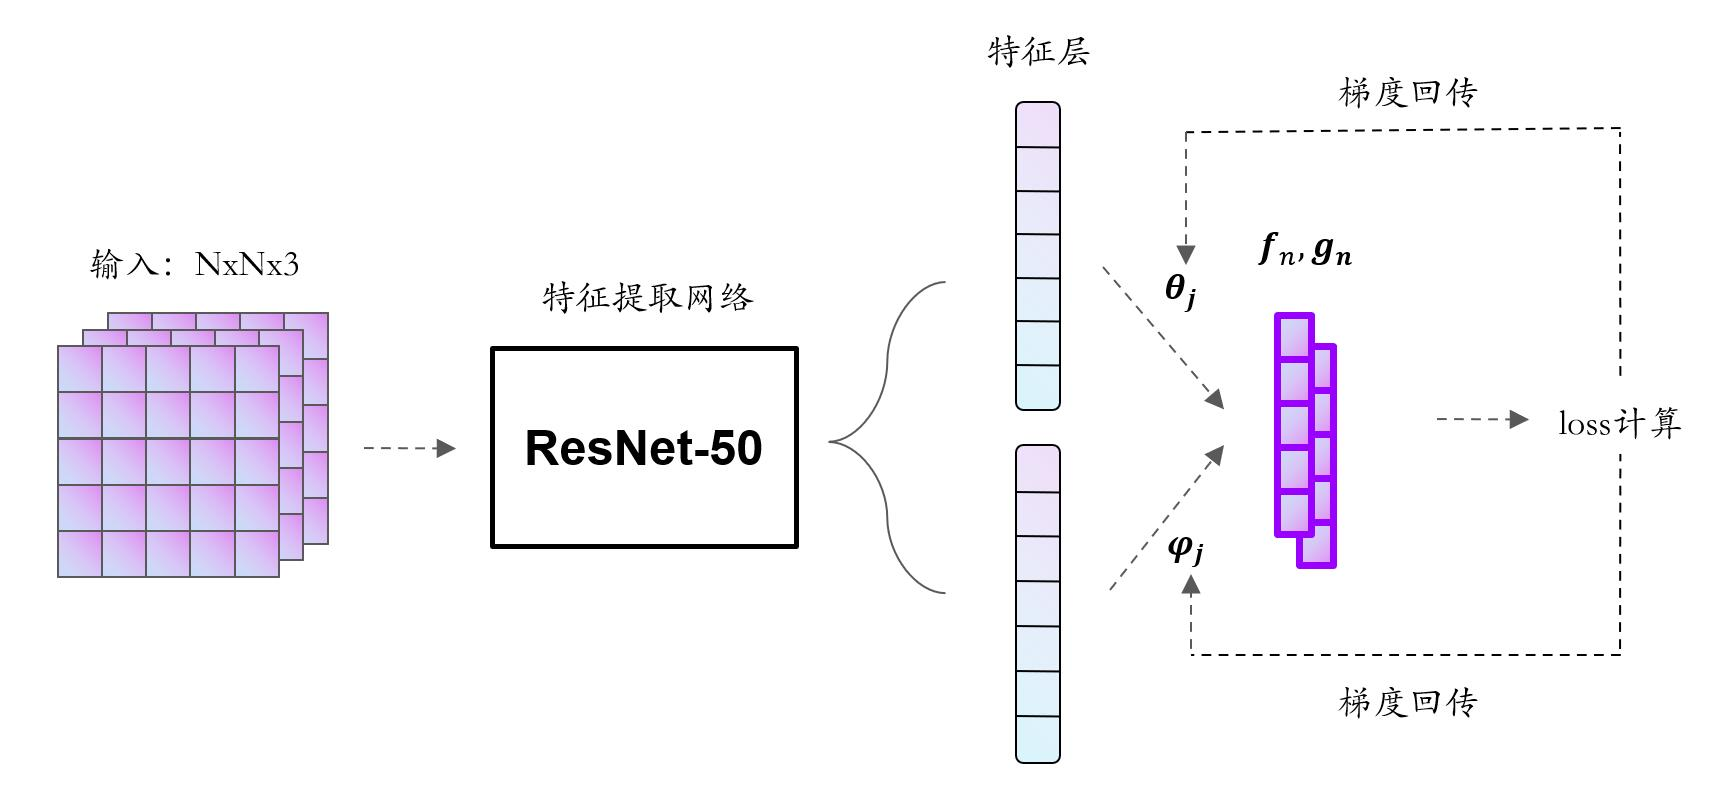
\includegraphics[width=1\linewidth]{char3_arc2_role_partial.jpg}
    \caption{\label{fig3:arc2}使用ResNet作为特征提取网络并使用标签预测策略的算法框架。}
\end{figure}

在此基础上将单个数据的标签预测向量记为${\boldsymbol g}_n$,各节点中所有数据的标签预测矩阵记为
${\boldsymbol G}_{\mathcal{N}_j}=\left[{\boldsymbol g}_n\right],n\in\mathcal{N}_j$。
有了强假设性的即时标签预测后,便可以采用监督学习中的交叉熵损失函数获得更多的信息。
将基于标签预测的强假设与上文基于期望正标签数量的弱假设式\eqref{PNR}进行结合,并辅以流形约束得到初步的RLE损失函数
$l_{\mathrm{RLE}}^{\prime}\left(\mathbf{F}_{\mathcal{N}_j} , {\mathbf{G}}_{\mathcal{N}_j}, \mathbf{Z}_{\mathcal{N}_j}\right)$:
\begin{equation}
    \label{RLE_temp1}
    \begin{split}
        l_{\mathrm{RLE}}^{\prime}\left(\mathbf{F}_{\mathcal{N}_j} , {\mathbf{G}}_{\mathcal{N}_j}, \mathbf{Z}_{\mathcal{N}_j}\right) 
        &=\frac{1}{N} \sum_{n \in \mathcal{N}_j} l_{\mathrm{BCE}}\left(\boldsymbol{f}_{n}, \operatorname{sg}\left({\boldsymbol{g}}_{n}\right)\right)
        +l_{\mathrm{PNR}}^l\left(\boldsymbol{F}_{\mathcal{N}_j^l}, \boldsymbol{Z}_{\mathcal{N}_j^l}\right) \\
        &+l_{\mathrm{PNR}}^{ul}\left(\boldsymbol{F}_{\mathcal{N}_j^{ul}}, \boldsymbol{Z}_{\mathcal{N}_j^{ul}}\right)
        +\frac{\sigma}{2\hat{N}_j} \sum_{n,m \in \hat{\mathcal{N}}_j}{ \omega_{nm} \sum_{i \in \mathcal{L}}\left({f}_{ni}-{f}_{mi}\right)^2 }
    \end{split}
\end{equation}
其中$\operatorname{sg}\left(\cdot \right)$是梯度中断函数,它将阻止梯度回传,使得${\boldsymbol{g}}_{n}$仅作为即时的预测标签来使用;
$l_{\mathrm{BCE}}$中的$\mathbb{I}_{\left[ g_{ni}=1\right]}$和$\mathbb{I}_{\left[g_{ni}=0\right]}$将根据
$g_{ni}\in\left[0,1\right]$的连续性分别修改为$g_{ni}$和$1-g_{ni}$;
最后一项流形约束项用以优化算法输出$\boldsymbol f_n$。
上述初步RLE损失函数$l_{\mathrm{RLE}}^{\prime}\left(\mathbf{F}_{\mathcal{N}_j} , {\mathbf{G}}_{\mathcal{N}_j}, \mathbf{Z}_{\mathcal{N}_j}\right)$
可在正类数量约束的基础上促使算法输出$\boldsymbol f_n$去接近预测标签${\boldsymbol g}_n$。

类似地,对标签预测$\boldsymbol g\left(\boldsymbol\varphi_j|\boldsymbol x\right)$的参数$\boldsymbol\varphi_j$进行优化,
只需要将式\eqref{RLE_temp1}中的标签预测${\mathbf{G}}_{\mathcal{N}_j}$与算法输出$\mathbf{F}_{\mathcal{N}_j}$的位置进行交换得到
$l^{\prime}\left(\mathbf{G}_{\mathcal{N}_j}, \mathbf{F}_{\mathcal{N}_j}, \mathbf{Z}_{\mathcal{N}_j}\right)$,即:
\begin{equation}
    \label{RLE_temp2}
    \begin{split}
        l_{\mathrm{RLE}}^{\prime}\left(\mathbf{G}_{\mathcal{N}_j}, \mathbf{F}_{\mathcal{N}_j}, \mathbf{Z}_{\mathcal{N}_j}\right) 
        &=\frac{1}{N} \sum_{n \in \mathcal{N}_j} l_{\mathrm{BCE}}\left(\boldsymbol{g}_{n}, 
        \operatorname{sg}\left({\boldsymbol{f}}_{n}\right)\right)
        +l_{\mathrm{PNR}}^l\left(\boldsymbol{G}_{\mathcal{N}_j^l}, \boldsymbol{Z}_{\mathcal{N}_j^l}\right) \\
        &+l_{\mathrm{PNR}}^{ul}\left(\boldsymbol{G}_{\mathcal{N}_j^{ul}}, \boldsymbol{Z}_{\mathcal{N}_j^{ul}}\right)
        +\frac{\sigma}{2\hat{N}_j} \sum_{n,m \in \hat{\mathcal{N}}_j}{ \omega_{nm} \sum_{i \in \mathcal{L}}\left({g}_{ni}-{g}_{mi}\right)^2 }.
    \end{split}
\end{equation}
需要指出的是,此处的最后一项流形约束项是用于优化标签预测输出$\boldsymbol g_n$, 而非如式\eqref{RLE_temp1}所示用以优化算法输出$\boldsymbol f_n$。

将$l^{\prime}\left(\mathbf{F}_{\mathcal{N}_j} , {\mathbf{G}}_{\mathcal{N}_j}, \mathbf{Z}_{\mathcal{N}_j}\right)$和
$l^{\prime}\left({\mathbf{G}}_{\mathcal{N}_j}, \mathbf{F}_{\mathcal{N}_j}, \mathbf{Z}_{\mathcal{N}_j}\right)$相结合,
{便可得到适用于SPUM数据的RLE损失函数,并构建网络上的全局优化问题为:
\begin{equation}
    \label{RLE_min}
    \begin{split}
        &\min_{\boldsymbol\theta_j,\boldsymbol\varphi_j}\frac{1}{J}\sum_{j\in\mathcal{J}}
        l_{\mathrm{RLE}}\left(\mathbf{F}_{\mathcal{N}_j} , {\mathbf{G}}_{\mathcal{N}_j}, \mathbf{Z}_{\mathcal{N}_j}\right) \\
        &=\min_{\boldsymbol\theta_j,\boldsymbol\varphi_j}\frac{1}{J}\sum_{j\in\mathcal{J}} \frac{1}{2} \left[
        l_{\mathrm{RLE}}^{\prime}\left(\mathbf{F}_{\mathcal{N}_j} , {\mathbf{G}}_{\mathcal{N}_j}, \mathbf{Z}_{\mathcal{N}_j}\right)
        +l_{\mathrm{RLE}}^{\prime}\left({\mathbf{G}}_{\mathcal{N}_j}, \mathbf{F}_{\mathcal{N}_j}, \mathbf{Z}_{\mathcal{N}_j}\right)
        \right].
    \end{split}
\end{equation}}

基于上述代价函数,可以通过同时训练输出函数$\boldsymbol f\left(\boldsymbol\theta_j,\boldsymbol x\right)$的参数$\boldsymbol\theta_j$和
标签预测$\boldsymbol g\left(\boldsymbol\varphi_j,\boldsymbol x\right)$的参数$\boldsymbol\varphi_j$对基于SPUM数据的学习问题进行优化,
并最终选取在测试集中表现最好的参数$\boldsymbol \theta_j$或$\boldsymbol\varphi_j$作为算法输出。

% Chapter 3.3
\section{分布式优化}\label{Char3_Distributed}
% Chapter 3.3.1
\subsection{分布式梯度下降}\label{Char3_DGD}
{基于\ref{Char3_LossDesign}节设计的全局优化问题式\eqref{ANLS_min}和式\eqref{RLE_min},本节将考虑如何在仅通过少量信息传递的情况下获得全局最优解。定义连接矩阵$\boldsymbol C=[C_{jb}],j,b\in\mathcal{J}$为数值化的分布式网络,}其中若节点$j$和$b$之间不存在无向连接的话有$C_{jb}=0$。
常用的一些分布式网络系数$C_{jb}$设计规则有Metropolis规则,拉普拉斯矩阵和均匀性规则等
\cite{Fang_Metropolis_2010, Olfati_Laplas_2004, Kang_Uniform_2021}。

以全局优化问题式\eqref{RLE_min}为例,每个节点都拥有自己独立的参数$\boldsymbol \theta_j$和$\boldsymbol \varphi_j$。
% \text { s.t. } \boldsymbol{\theta}_{j}=\boldsymbol{\theta}_{b},\boldsymbol{\varphi}_{j}=\boldsymbol{\varphi}_{b},
% j \in \mathcal{J}, b \in \mathcal{B}_{j}
使用$\boldsymbol W_j=\left[\boldsymbol\theta_j,\boldsymbol\varphi_j\right]$代表本地节点的参数向量。
基于上文提及的无向图网络$\mathcal{G}=\left\{\mathcal{J},\mathcal{B}\right\}$和连接矩阵$\boldsymbol C=[C_{jb}]$,本文可以使用
分布式梯度下降(distributed gradient decent, DGD)\cite{Scardapane_Distributed_2016}去融合节点间的暂态参数估计矩阵,
从而解决式\eqref{RLE_min}所表示的分布式优化问题。
其具体做法为对每个数据节点进行如下迭代步骤:
\begin{subequations}
    \label{DGD}
    \begin{align}
        &\boldsymbol\varPsi_j\left(t-1\right)=\boldsymbol W_j\left(t-1\right)-
        \eta\left(t-1\right)\nabla_{\boldsymbol W_j}\left(l_{\mathrm{RLE}}\right)\left|_{\boldsymbol W_j\left(t-1\right)}\right.,
        \label{DGD_1} \\
        &\boldsymbol W_j\left(t\right)=\sum_{k=1}^{J}C_{jk}\boldsymbol\varPsi_k\left(t-1\right), \label{DGD_2}
    \end{align}
\end{subequations}
其中$\boldsymbol W_j\left(t\right)$为第$t$次迭代时的本地参数向量,
$\nabla_{\boldsymbol W_j}\left(l_{\mathrm{RLE}}\right)\left|_{\boldsymbol W_j\left(t\right)}\right.$为损失函数$l_{\mathrm{RLE}}$
在第$t$次迭代时关于$\boldsymbol W_j\left(t\right)$的导数且$t\in\mathcal{T}=\left\{1,2,...T\right\}$;
$\boldsymbol\varPsi_j\left(t\right)$为本地节点在第$t$次迭代时的暂态参数估计矩阵;
$\eta\left(t\right)\in\left(0,1\right]$是随时间变化的学习率超参数,满足消逝条件\cite{Bottou_Vanish1_2010,Shalev_Vanish2_2011}:
\begin{equation}
    \label{VanishCondition}
    \begin{split}
        \sum_{t=1}^{+\infty}{\eta\left(t\right)}=+\infty, ~\sum_{t=1}^{+\infty}{\eta\left(t\right)}^2<+\infty.
    \end{split}
\end{equation}
那么若整个网络是强连通的,则每个节点之间的信息便可以在网络之间进行交流传输,最终实现一致最优\cite{Geary_Incremental_1999}。

在式\eqref{DGD}中,式\eqref{DGD_1}表示了本地节点暂态参数估计矩阵的更新过程,在本地节点更新之后,其暂态参数估计矩阵将被传输到邻居节点中,
各节点再根据邻居节点传输过来的各暂态参数估计矩阵,通过式\eqref{DGD_2}进行加权组合得到最终的本地参数向量$\boldsymbol W_j\left(t\right)$。
在传递关键信息的同时不涉及到原始数据之间的相互传递,有效保护了各节点之间的隐私性。
基于分布式梯度下降算法,初步完成基于SPUM数据的分布式SPUM学习(distributed single positive and unlabeled multi-label learning,dSPUM)算法,
其具体算法实现过程可以总结为\autoref{dSSML_eventTrigger_ori}。
dSPUM算法中式\eqref{DGD_1}中的损失函数$l_{\mathrm{RLE}}$将会在仿真中更换为已提及过的两个损失函数并进行探索,并且使用$l_{\mathrm{ANLS}}$时参数向量$\boldsymbol W_j=\boldsymbol \theta_j$。

\begin{algorithm}[htbp]
	\caption{分布式SPUM学习
    (distributed single positive and unlabeled multi-label learning,dSPUM)算法}
	\label{dSSML_eventTrigger_ori}
	\LinesNumbered
	\KwIn{各节点经过特征提取网络得到的的训练数据 $\boldsymbol{X}_j, j \in \mathcal{J}$}
	\KwOut{各节点训练后的最优模型参数 $\boldsymbol{W}_j, j \in \mathcal{J}$}
	{随机初始化各节点的模型参数$\boldsymbol{W}_j\left(0\right), j \in \mathcal{J}$};\\
	\For{$t=1\in\mathcal{T}$}{
        \For{$j \in \mathcal{J}$}{  
            通过式\eqref{DGD_1}更新本地节点$j$的暂态参数估计矩阵$\boldsymbol\varPsi_j\left(t-1\right)$;\\
            将节点的暂态参数估计矩阵$\boldsymbol\varPsi_j\left(t-1\right)$传送到邻居节点。
        }
        \For{$j \in \mathcal{J}$}{
            通过式\eqref{DGD_2}加权组合各邻居节点的暂态参数估计矩阵来更新本地节点$j$的参数向量$\boldsymbol W_j\left(t\right)$;
        }
    }
\end{algorithm}

% 改写这个了,看苗雪丹的毕业论文中有详细的证明
% Chapter 3.3.2
\subsection{收敛性分析}\label{Char3_Conv}
本节将对所提分布式算法进行收敛性分析,在此之前首先给出两条在分布式处理中常用的假设条件。
\begin{assumption} 
    所考虑的分布式网络$\mathcal{J}$是强连通的,此外连接矩阵$\boldsymbol C$满足$\boldsymbol C \boldsymbol1=\boldsymbol1$
    且$\boldsymbol1^T\boldsymbol C=\boldsymbol1^T$,其中$\boldsymbol1$表示所有值均为$\mathrm{1}$的$J$维向量。
    
    注:文献中提出了诸多满足本假设的连接向量值$\left\{C_{jb}\right\}$设计准则,如$\mathrm{Metroplis}$准则\rm{\cite{Fang_Metropolis_2010}},拉普拉斯矩阵\rm{\cite{Olfati_Laplas_2004}}和一致性准则\rm{\cite{Kang_Uniform_2021}}等。
\end{assumption}
\begin{assumption}
    各节点的目标损失函数序列$\left.l\right|_{\boldsymbol{W}_j\left(t\right)}$是一致有界的,
    且其梯度$\left.\nabla_{\boldsymbol{W}_j} \left(l\right)\right|_{\boldsymbol{W}_j\left(t\right)}$序列也是一致有界的。
\end{assumption}

基于上述\textbf{假设 1},\textbf{假设 2}和消逝条件式\eqref{VanishCondition},对dSPUM算法的收敛性进行分析。
% 将证明在$t\to\infty$时各节点参数。
将式\eqref{DGD_1}和式\eqref{DGD_2}结合,可将$\boldsymbol W_j\left(t\right)$的迭代更新公式重写为:
\begin{equation}
    \label{DGD_Sum}
    \boldsymbol W_j\left(t\right)=\sum_{k=1}^{J}C_{jk} \left[
    \boldsymbol W_j\left(t-1\right)-\eta\left(t-1\right)\nabla_{\boldsymbol W_j}\left(l\right)\left|_{\boldsymbol W_j\left(t-1\right)}\right. \right].
\end{equation}
{将各节点的参数向量叠加得到全局参数矩阵$\boldsymbol{\mathcal{W}}\left(t\right)=\left[\boldsymbol W_1\left(t\right)~\boldsymbol W_2\left(t\right)~...~\boldsymbol W_J\left(t\right)\right]^T$
,梯度向量叠加得到全局梯度矩阵$\boldsymbol{\nabla}\left(t\right)=-\left[\nabla_{\boldsymbol W_1}\left(l\right)\left|_{\boldsymbol W_1\left(t\right)}\right.~\nabla_{\boldsymbol W_2}\left(l\right)\left|_{\boldsymbol W_2\left(t\right)}\right.~...~\nabla_{\boldsymbol W_T}\left(l\right)\left|_{\boldsymbol W_T\left(t\right)}\right.~\right]^T$
。}则式\eqref{DGD_Sum}可被改写为矩阵形式:
\begin{equation}
    \label{DGD_Sum_M}
    \boldsymbol{\mathcal{W}}\left(t\right)=\boldsymbol C \left[
    \boldsymbol{\mathcal{W}}\left(t-1\right)+\eta\left(t-1\right)\boldsymbol{\nabla}\left(t-1\right)
    \right].
\end{equation}
根据\textbf{假设 1},全局参数与节点间的平均参数$\overline{\boldsymbol W}\left(t\right)=\frac{1}{J}\boldsymbol1\boldsymbol1^T\boldsymbol W\left(t\right)$
之间的差值可化简为:
\begin{equation}
    \label{DisOfWW}
    \begin{split}
        \boldsymbol{\mathcal{W}}\left(t\right) - \frac{1}{J}\boldsymbol1\boldsymbol1^T\boldsymbol W\left(t\right)
        &=\left(\boldsymbol I-\frac{1}{J}\boldsymbol1\boldsymbol1^T\right)\boldsymbol{\mathcal{W}}\left(t\right) \\
        &=\left(\boldsymbol I-\frac{1}{J}\boldsymbol1\boldsymbol1^T\right)\boldsymbol C\left[
            \boldsymbol{\mathcal{W}}\left(t-1\right)+\eta\left(t-1\right)\boldsymbol{\nabla}\left(t-1\right)
        \right] \\
        &=\left(\boldsymbol C-\frac{1}{J}\boldsymbol1\boldsymbol1^T\right)\boldsymbol{\mathcal{W}}\left(t-1\right)
        +\left(\boldsymbol C-\frac{1}{J}\boldsymbol1\boldsymbol1^T\right)\eta\left(t-1\right)\boldsymbol{\nabla}\left(t-1\right),
    \end{split}
\end{equation}
其中式\eqref{DisOfWW}最后一个等式的第一项可被进一步改写为:
\begin{equation}
    \label{DOW_temp_1}
    \begin{split}
        \left(\boldsymbol C-\frac{1}{J}\boldsymbol1\boldsymbol1^T\right)\boldsymbol{\mathcal{W}}\left(t-1\right)
        &=\left(\boldsymbol C-\frac{1}{J}\boldsymbol1\boldsymbol1^T\right)\boldsymbol{\mathcal{W}}\left(t-1\right)
        - \frac{1}{J}\boldsymbol1\boldsymbol1^T\boldsymbol {\mathcal{W}}\left(t-1\right) 
        + \frac{1}{J}\boldsymbol1\boldsymbol1^T\boldsymbol {\mathcal{W}}\left(t-1\right) \\
        &=\left(\boldsymbol C-\frac{1}{J}\boldsymbol1\boldsymbol1^T\right)
        \left[\boldsymbol{\mathcal{W}}\left(t-1\right) - \frac{1}{J}\boldsymbol1\boldsymbol1^T\boldsymbol{\mathcal{W}}\left(t-1\right)\right].
    \end{split}
\end{equation}
将式\eqref{DOW_temp_1}代入到式\eqref{DisOfWW},可以得到:
\begin{equation}
    \label{DisOfWW_2}
    \begin{split}
        &\boldsymbol{\mathcal{W}}\left(t\right) - \frac{1}{J}\boldsymbol1\boldsymbol1^T\boldsymbol W\left(t\right)   \\
        &=\left(\boldsymbol C-\frac{1}{J}\boldsymbol1\boldsymbol1^T\right)
        \left[\boldsymbol{\mathcal{W}}\left(t-1\right) - \frac{1}{J}\boldsymbol1\boldsymbol1^T\boldsymbol{\mathcal{W}}\left(t-1\right)\right]
        +\left(\boldsymbol C-\frac{1}{J}\boldsymbol1\boldsymbol1^T\right)\eta\left(t-1\right)\boldsymbol{\nabla}\left(t-1\right)    \\
        &= \left(\boldsymbol C-\frac{1}{J}\boldsymbol1\boldsymbol1^T\right) \left[
            \boldsymbol{\mathcal{W}}\left(t-1\right) - \frac{1}{J}\boldsymbol1\boldsymbol1^T\boldsymbol{\mathcal{W}}\left(t-1\right)
            +\eta\left(t-1\right)\boldsymbol{\nabla}\left(t-1\right)
        \right].
    \end{split}
\end{equation}
对式\eqref{DisOfWW_2}两边取范数,得到:
\begin{equation}
    \label{DisOfWW_3}
    \begin{split}
        &\left\|\boldsymbol{\mathcal{W}}\left(t\right) - \frac{1}{J}\boldsymbol1\boldsymbol1^T\boldsymbol{\mathcal{W}}\left(t\right)\right\| \\
        &~~~~~~~~
        =\left\|\left(\boldsymbol C-\frac{1}{J}\boldsymbol1\boldsymbol1^T\right) \left[
            \boldsymbol{\mathcal{W}}\left(t-1\right) - \frac{1}{J}\boldsymbol1\boldsymbol1^T\boldsymbol{\mathcal{W}}\left(t-1\right)
            +\eta\left(t-1\right)\boldsymbol{\nabla}\left(t-1\right)
        \right]\right\|   \\
        &~~~~~~~~
        \leq\left\|\left(\boldsymbol C-\frac{1}{J}\boldsymbol1\boldsymbol1^T\right) \right\| \cdot
        \left\|\left[
            \boldsymbol{\mathcal{W}}\left(t-1\right) - \frac{1}{J}\boldsymbol1\boldsymbol1^T\boldsymbol{\mathcal{W}}\left(t-1\right)
            +\eta\left(t-1\right)\boldsymbol{\nabla}\left(t-1\right)
        \right]\right\|   \\
        &~~~~~~~~
        \leq r \left\|\boldsymbol{\mathcal{W}}\left(t-1\right) - \frac{1}{J}\boldsymbol1\boldsymbol1^T\boldsymbol {\mathcal{W}}\left(t-1\right)\right\|
        +r \eta\left(t-1\right)\left\|\boldsymbol{\nabla}\left(t-1\right)\right\| ,
    \end{split}
\end{equation}
其中$r=\left\|\left(\boldsymbol C-\frac{1}{J}\boldsymbol1\boldsymbol1^T\right) \right\|<1$。

根据\textbf{假设 2},必然存在一个有限正数$G$作为$\nabla_{\boldsymbol W_j}\left(l\right)\left|_{\boldsymbol W_j\left(t\right)}\right.$的上界,即$\left\|\nabla_{\boldsymbol W_j}\left(l\right)\left|_{\boldsymbol W_j\left(t\right)}\right.\right\|\leq G,~\text{for all}~
j\in\mathcal{J},t\in\mathcal{T}$,则有$\left\|\boldsymbol{\nabla}\left(t-1\right)\right\|\leq JG$。因此式\eqref{DisOfWW_3}可被重写为:
\begin{equation}
    \label{DisOfWW_4}
    \left\|\boldsymbol{\mathcal{W}}\left(t\right) - \frac{1}{J}\boldsymbol1\boldsymbol1^T\boldsymbol{\mathcal{W}}\left(t\right)\right\|    \leq
    r \left\|\boldsymbol{\mathcal{W}}\left(t-1\right) - \frac{1}{J}\boldsymbol1\boldsymbol1^T\boldsymbol {\mathcal{W}}\left(t-1\right)\right\|
    + r\eta\left(t-1\right)JG.
\end{equation}
令$d\left(t\right)=\left\|\boldsymbol{\mathcal{W}}\left(t\right) - \frac{1}{J}\boldsymbol1\boldsymbol1^T\boldsymbol{\mathcal{W}}\left(t\right)\right\|\geqslant0$
,即可由式\eqref{DisOfWW_4}得到:
\begin{equation}
    \label{DisOfWW_5}
    d\left(t\right) \leq r\left[(d\left(t-1\right)+\eta\left(t-1\right)JG\right].
\end{equation}
构建辅助变量$s\left(t\right)=r\left[s\left(t-1\right)+\eta\left(t-1\right)JG\right]$,且设置$s\left(0\right)=d\left(0\right)\geqslant0$。
则结合式\eqref{DisOfWW_5}易推得:
\begin{equation}
    \label{temp_sd_1}
    s\left(1\right)=r\left[s\left(0\right)+\eta\left(0\right)JG\right]
    =r\left[d\left(0\right)+\eta\left(0\right)JG\right] \geqslant d\left(1\right),
\end{equation}
同理可得$s\left(2\right) \geqslant d\left(1\right)$,循环进行数学归纳则可推出,对每一个时刻$t\in\mathcal{T}$,都有:
\begin{equation}
    \label{temp_s}
    s\left(t\right) \geqslant d\left(t\right) \geqslant 0,~\text{for all}~t \in \mathcal{T}.
\end{equation}

假设存在某一时刻$t'$,使得$s\left(t'\right)\geqslant\frac{\eta\left(t'\right)JG}{\frac{1}{r}-1}$,
则根据$s\left(t\right)=r\left[s\left(t-1\right)+\eta\left(t-1\right)JG\right]$可以推出:
\begin{equation}
    \label{Last_1}
    \begin{split}
        s\left(t'\right) &= r\left[(s\left(t'-1\right)+\eta\left(t'-1\right)JG\right] 
        \leq r\left[
            s\left(t'-1\right) + \left(\frac{1}{r}-1\right)s\left(t'-1\right)
        \right]=s\left(t'-1\right).
    \end{split}
\end{equation}
则由式\eqref{Last_1}可归纳得到当$t\geqslant t'$时,有:
\begin{equation}
    \label{Last_2}
    s\left(t-1\right) \geqslant s\left(t\right) \geqslant 0,
\end{equation}
即序列$s\left(t\right)$单调递减。
由学习率$\eta\left(t\right)$的消逝条件式\eqref{VanishCondition}易得$\lim_{t\to\infty}\eta\left(t\right)=0$
,然后对$s\left(t\right)=r\left[s\left(t-1\right)+\eta\left(t-1\right)JG\right]$两边对$t$取极限,得到:
\begin{equation}
    \label{Last_3}
    \lim_{t\to\infty}s\left(t\right)=\lim_{t\to\infty}r\left[s\left(t-1\right)+\eta\left(t-1\right)JG\right]
    =\lim_{t\to\infty}rs\left(t-1\right).
\end{equation}
由式\eqref{Last_2}可知序列$s\left(t\right)$单调递减且有下界为0,并且由式\eqref{Last_3}可知
$\lim_{t\to\infty}s\left(t\right)=\lim_{t\to\infty}rs\left(t-1\right),r<1$即$s\left(t\right)$在$t\to\infty$时成比例下降,
则易推出$\lim_{t\to\infty}s\left(t\right)=0$。
则基于\eqref{temp_s}对$s\left(t\right)$和$d\left(t\right)$同时关于$t$取极限,得到:
\begin{equation}
    \label{Last_4}
    0=\lim_{t\to\infty}s\left(t\right) \geqslant \lim_{t\to\infty}d\left(t\right) \geqslant 0,
\end{equation}
则根据夹逼定理易得$\lim_{t\to\infty}d\left(t\right)=0$。
而若不存在任一时刻$t'$满足$s\left(t'\right)\geqslant\frac{\eta\left(t'\right)JG}{\frac{1}{r}-1}$,则既是对于
任意时刻$t>0$,都有$s\left(t\right)<\frac{\eta\left(t\right)JG}{\frac{1}{r}-1}$,对$t$取极限且根据$\lim_{t\to\infty}\eta\left(t\right)=0$得;
\begin{equation}
    \label{Last_5}
    0<\lim_{t\to\infty}s\left(t\right)<\lim_{t\to\infty}\frac{\eta\left(t\right)JG}{\frac{1}{r}-1}=0,
\end{equation}
根据夹逼定理易得$\lim_{t\to\infty}s\left(t\right)=0$,同理也可推出$\lim_{t\to\infty}d\left(t\right)=0$。

基于以上推导本文最终证明了,在$t\to\infty$时有$\lim_{t\to\infty}d\left(t\right)=0$,即:
\begin{equation}
    \label{Last_last}
    \lim_{t\to\infty}\left\|\boldsymbol{\mathcal{W}}\left(t\right) 
    - \frac{1}{J}\boldsymbol1\boldsymbol1^T\boldsymbol{\mathcal{W}}\left(t\right)\right\|=0,
\end{equation}
其中$\boldsymbol{\mathcal{W}}\left(t\right)- \frac{1}{J}\boldsymbol1\boldsymbol1^T\boldsymbol{\mathcal{W}}\left(t\right)$
的第$j$行表示$\boldsymbol W_j\left(t\right)-\overline{\boldsymbol W}\left(t\right)$,
$\overline{\boldsymbol W}\left(t\right)=\frac{1}{J}\sum_{j\in\mathcal{J}}\boldsymbol W_j\left(t\right)$为各节点参数的平均值。
因此根据式\eqref{Last_last},对于所有的节点$j\in\mathcal{J}$在$t\to\infty$时都有
$\lim_{t\to\infty}\left\|\boldsymbol W_j\left(t\right)-\overline{\boldsymbol W}\left(t\right)\right\|=0$,
即在$t\to\infty$时各节点的参数$\boldsymbol W_j\left(t\right)$将一致收敛至$\overline{\boldsymbol W}\left(t\right)$。

% Chapter 3.3.3
\subsection{事件触发策略}
上述\ref{Char3_DGD}节基于分布式梯度下降算法,给出了针对SPUM数据的分布式学习算法。
但在通信带宽等资源受限的分布式网络中,由于$\boldsymbol\varPsi_j\left(t\right)$的规模可能会非常大,若每一次迭代时都将其传输至邻居节点会
造成较大的通信代价\cite{Li_Event_2015, Ge_Event_2020}。
为了减少邻居节点间的通信负担,本文采用了事件触发的迭代策略,根据当前信息量的大小,决定信息的传递与否。
这种策略在自动控制、系统状态调控领域中已被广泛研究应用\cite{Gao_Event_2021, Liang_Event_2020}。

在本节的分布式场景中,本文将定义一个事件,并让其决定本地节点的$\boldsymbol\varPsi_j\left(t\right)$是否会被网络传输到邻居节点。
其中定义$\boldsymbol\varPsi_j\left(t_j^{event}\right)$为上一次被允许传输的暂态参数估计矩阵,$t_j^{event}$为节点$j$上一次被允许传输的时间点。
{将事件定义为$\boldsymbol\varPsi_j\left(t\right)$相比于$\boldsymbol\varPsi_j\left(t_j^{event}\right)$的变化率,
因变化率越大则其信息量也越大。当变化率大于阈值$\delta$时,认为所含信息量较大,节点之间进行信息的传输。例如,针对节点$j$而言,当}
\begin{equation}
    \label{event_trigger}
    \frac{\left\|\boldsymbol\varPsi_j\left(t\right) - \boldsymbol\varPsi_j\left(t_j^{event}\right)\right\|_2}
    {\left\|\boldsymbol\varPsi_j\left(t_j^{event}\right)\right\|_2} > \delta
\end{equation}
{的时候,节点$j$被允许向邻居节点传递信息。}
若此事件在节点$j$上被触发,那么触发事件时间点$t_j^{event}$将被更新为$t$,相应的被允许传输的暂态参数估计矩阵
$\boldsymbol\varPsi_j\left(t_j^{event}\right)$也将被替换为$\boldsymbol\varPsi_j\left(t\right)$并将其传输至邻居节点。
本文将基于事件触发策略的dSPUM学习算法的具体实现过程总结为\autoref{dSSML_eventTrigger}。
\begin{algorithm}[htbp]
	\caption{基于事件触发策略的dSPUM学习算法}
	\label{dSSML_eventTrigger}
	\LinesNumbered
	\KwIn{各节点经过特征提取网络得到的的训练数据 $\boldsymbol{X}_j, j \in \mathcal{J}$}
	\KwOut{{各节点训练后的最优模型参数 $\boldsymbol{W}_j^*, j \in \mathcal{J}$}}
	{随机初始化各节点的模型参数$\boldsymbol{W}_j\left(0\right), j \in \mathcal{J}$};\\
	\For{$t\in\mathcal{T}$}{
        \For{$j \in \mathcal{J}$}{  
            通过式\eqref{DGD_1}更新本地节点$j$的暂态参数估计矩阵$\boldsymbol\varPsi_j\left(t-1\right)$;\\
            \eIf{节点$j$满足式\eqref{event_trigger}}{
                触发事件时间点$t_j^{event}$将被更新为$t-1$; \\
                被允许传输的暂态参数估计矩阵$\boldsymbol\varPsi_j\left(t_j^{event}\right)$
                被更新为$\boldsymbol\varPsi_j\left(t-1\right)$; \\
                $\boldsymbol\varPsi_j\left(t_j^{event}\right)$被传输至邻居节点;
            }{$t_j^{event}$和$\boldsymbol\varPsi_j\left(t_j^{event}\right)$保持不变;}
        }
        \For{$j \in \mathcal{J}$}{  
            通过式\eqref{DGD_2}加权组合各邻居节点的暂态参数估计矩阵来更新本地节点$j$的参数向量$\boldsymbol W_j\left(t\right)$;
        }
    }
\end{algorithm}

% Char3.4
\section{仿真实验与结果}\label{Char3_Experiments}
在本节中,我们使用均值平均查准率(mean average precision,mAP)作为评价算法性能的主要指标,下面简单介绍其计算方式。
在对图片进行标签输出时,将设置一个置信度阈值$p_c\in\left[0,1\right]$使用$f_{ni} > p_c,i\in\mathcal{L}$判断该图片是否属于类别$i$。
对每一个类别$i$,根据不同的置信度阈值$p_c$将会分别得到不同的查准率(Precision$_i$)和召回率(Recall$_i$),其分别定义为:
\begin{equation}
    \label{PandR}
    \begin{split}
        \text{Precision}_i = \frac{TP_i}{TP_i+FP_i}, \\
        \text{Recall}_i = \frac{TP_i}{TP_i+FN_i},
    \end{split}
\end{equation}
其中$TP_i$表示$i$类正例中被正确判断为正例的个数,$FP_i$表示$i$类负例中被错误判断为正例的个数,
$FN_i$表示$i$类正例中被错误判断为负例的个数。
根据不同置信度阈值$p_c$得到的诸多Precision$_i$和Recall$_i$可绘制出二维PR曲线,计算此曲线下的面积即可得到$i$类的平均查准率
(average precision, AP$_i$)。
均值平均查准率mAP可通过计算所有类别的AP$_i$的平均值得到,即:
\begin{equation}
    \label{mAP}
    \text{mAP}=\frac{1}{L}\sum_{i\in\mathcal{L}}\text{AP}_i.
\end{equation}

{此外,为了探寻不同标注率情况下算法的性能,在本节定义一个指标LTR来表述标注数据占总数据的比例,即:}
\begin{equation}
    \label{LTR}
    \mathrm{LTR}=\frac{\text{标注数据的数量}}{\text{数据总数量}}\times100\%,
\end{equation}
其中每个标注数据都为单正例无标注的多标签数据。

\begin{figure}[htbp]
    \centering
    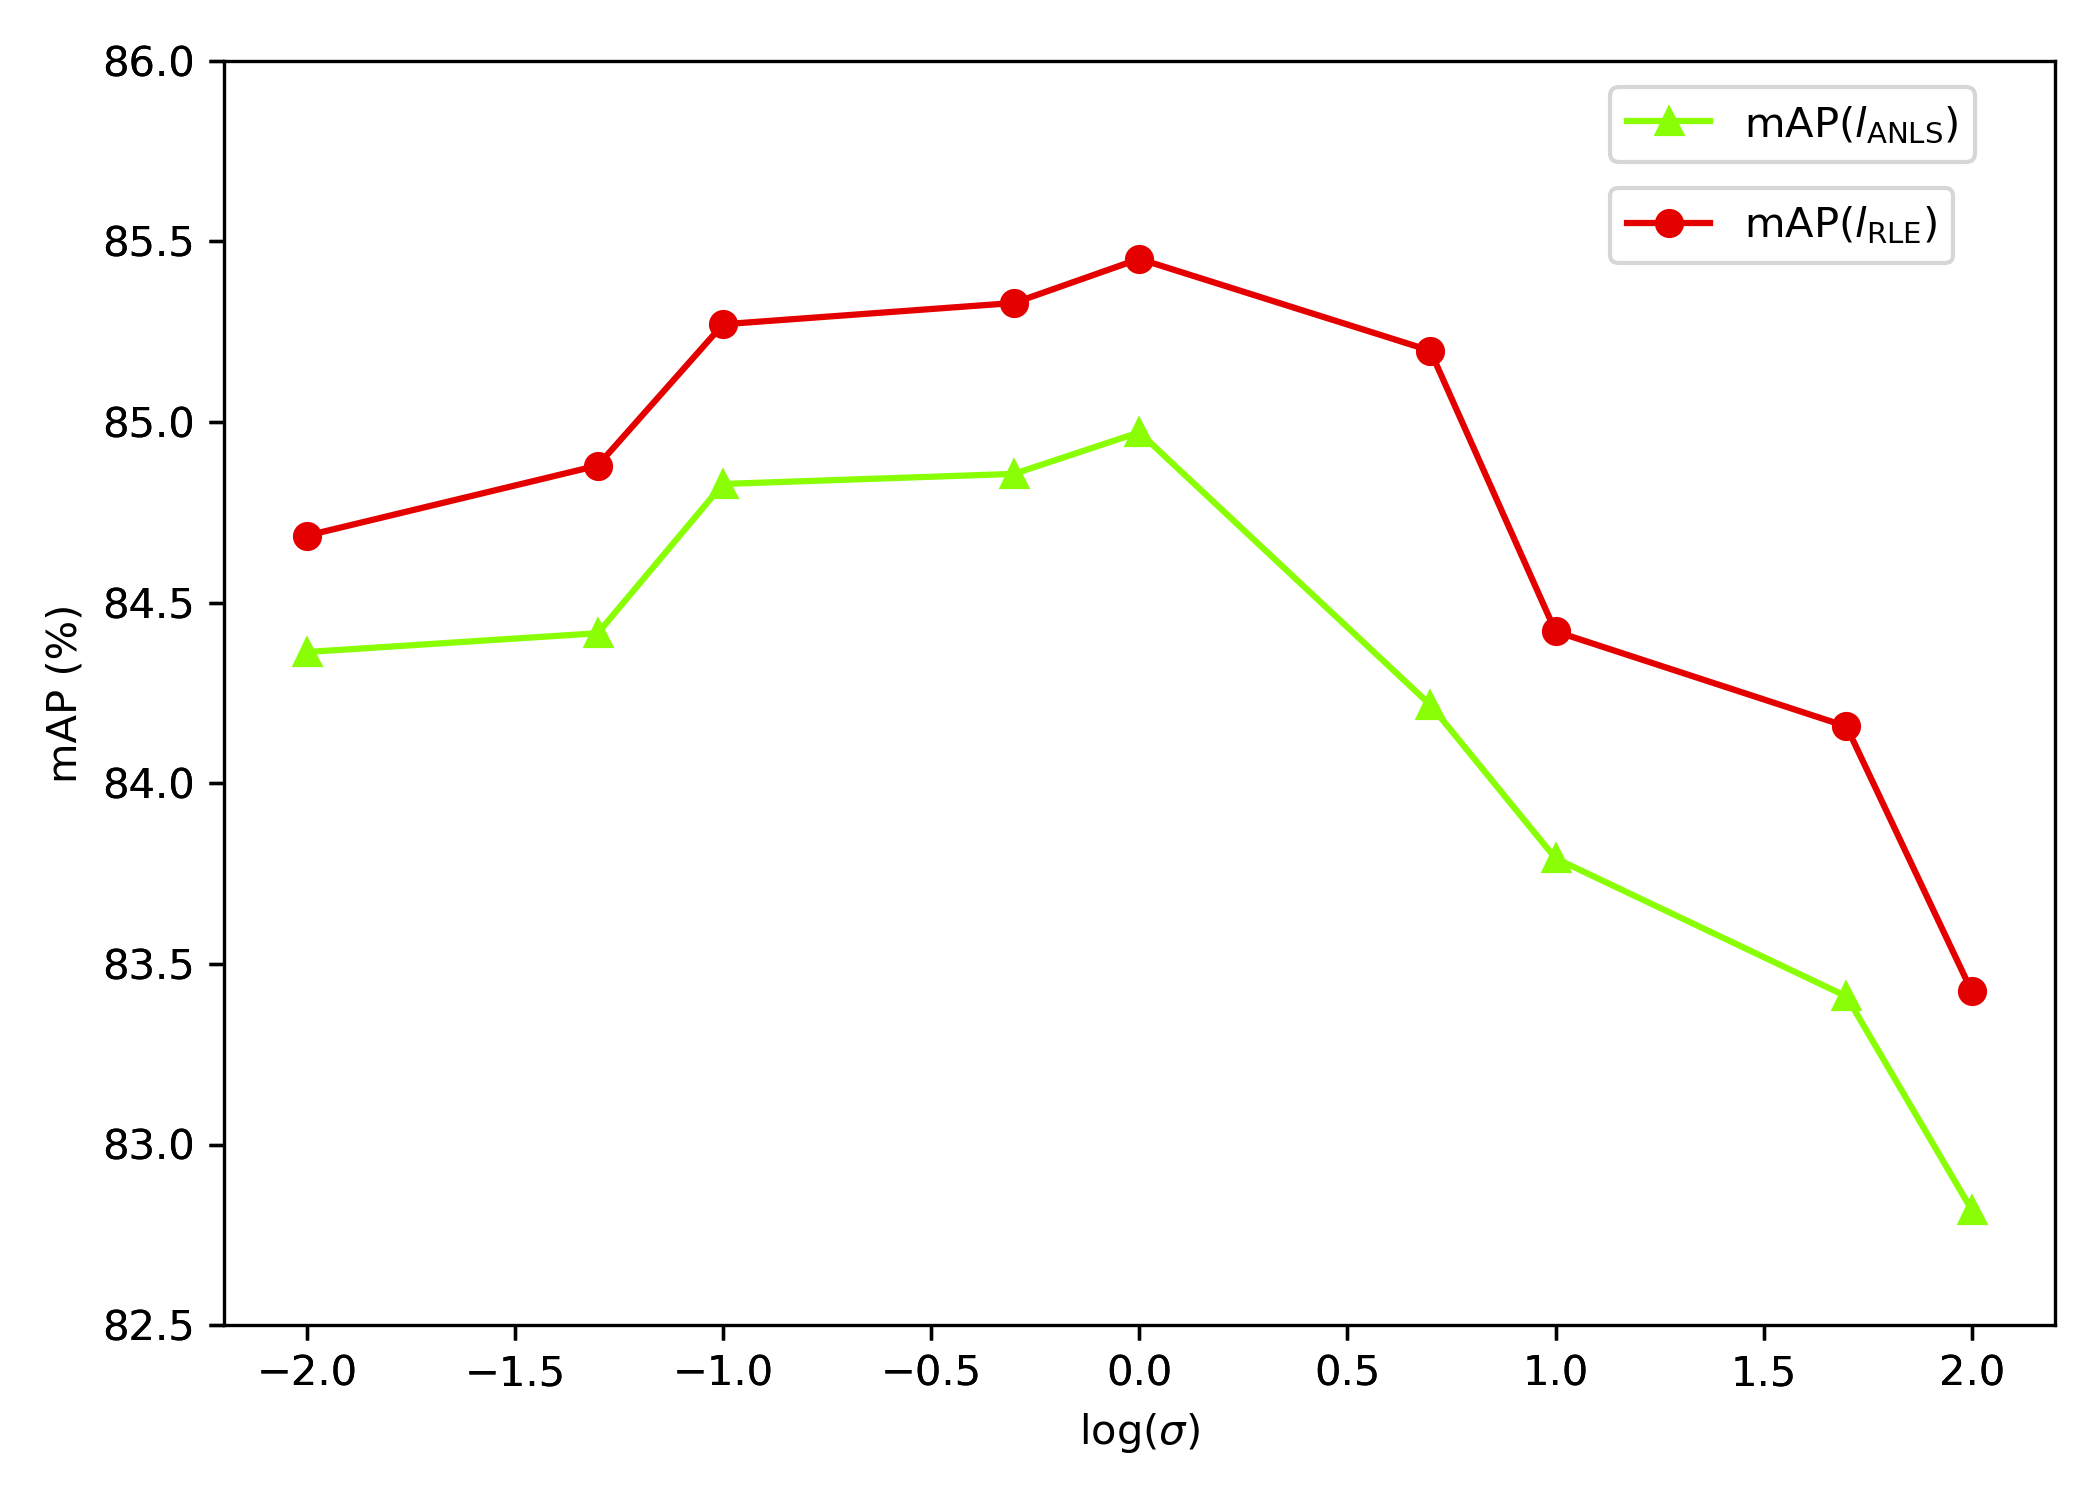
\includegraphics[width=0.7\linewidth]{char3_sigma.png}
    \caption{\label{fig3:sigma}在$Pascal~Voc$数据集上,LTR=60\%时dSPUM算法基于不同损失函数在不同比例参数$\sigma$下的mAP值。}
\end{figure}

\subsection{参数选取}
本文首先使用含有5717个训练图片、5823个测试图片和20个类别标签的$Pascal~Voc$数据集进行多种情况的实验仿真,去探索各参数的合适取值。
根据不同的LTR设置将数据$\mathcal{N}$划分为已标注数据集$\mathcal{N}^{l}$和未标注数据集$\mathcal{N}^{ul}$,并随机分配到20个节点中去
(每个节点有$\mathcal{N}_j^{l}$和$\mathcal{N}_j^{ul}$)。
其中对于已标注数据集$\mathcal{N}_j^{l}$的每一个样本的标签观测值都会被随机抽取一个保存为$z_{ni}=+1$,
其余各标签观测值则都置为$z_{ni}=\varnothing$。
对于未标注数据集$\mathcal{N}_j^{ul}$的每一个样本的每一个标签观测值都会置为
$z_{ni}=\varnothing, \text{for all}~i\in\mathcal{L}$。
本节仿真中学习率将被设置为${e^{-5}}/\left(t+1\right)$,并对基于两种损失函数$l_{\mathrm{ANLS}}$和$l_{\mathrm{RLE}}$的
的dSPUM算法的测试结果取50次仿真的平均值。

\begin{figure}[htbp]
    \centering
    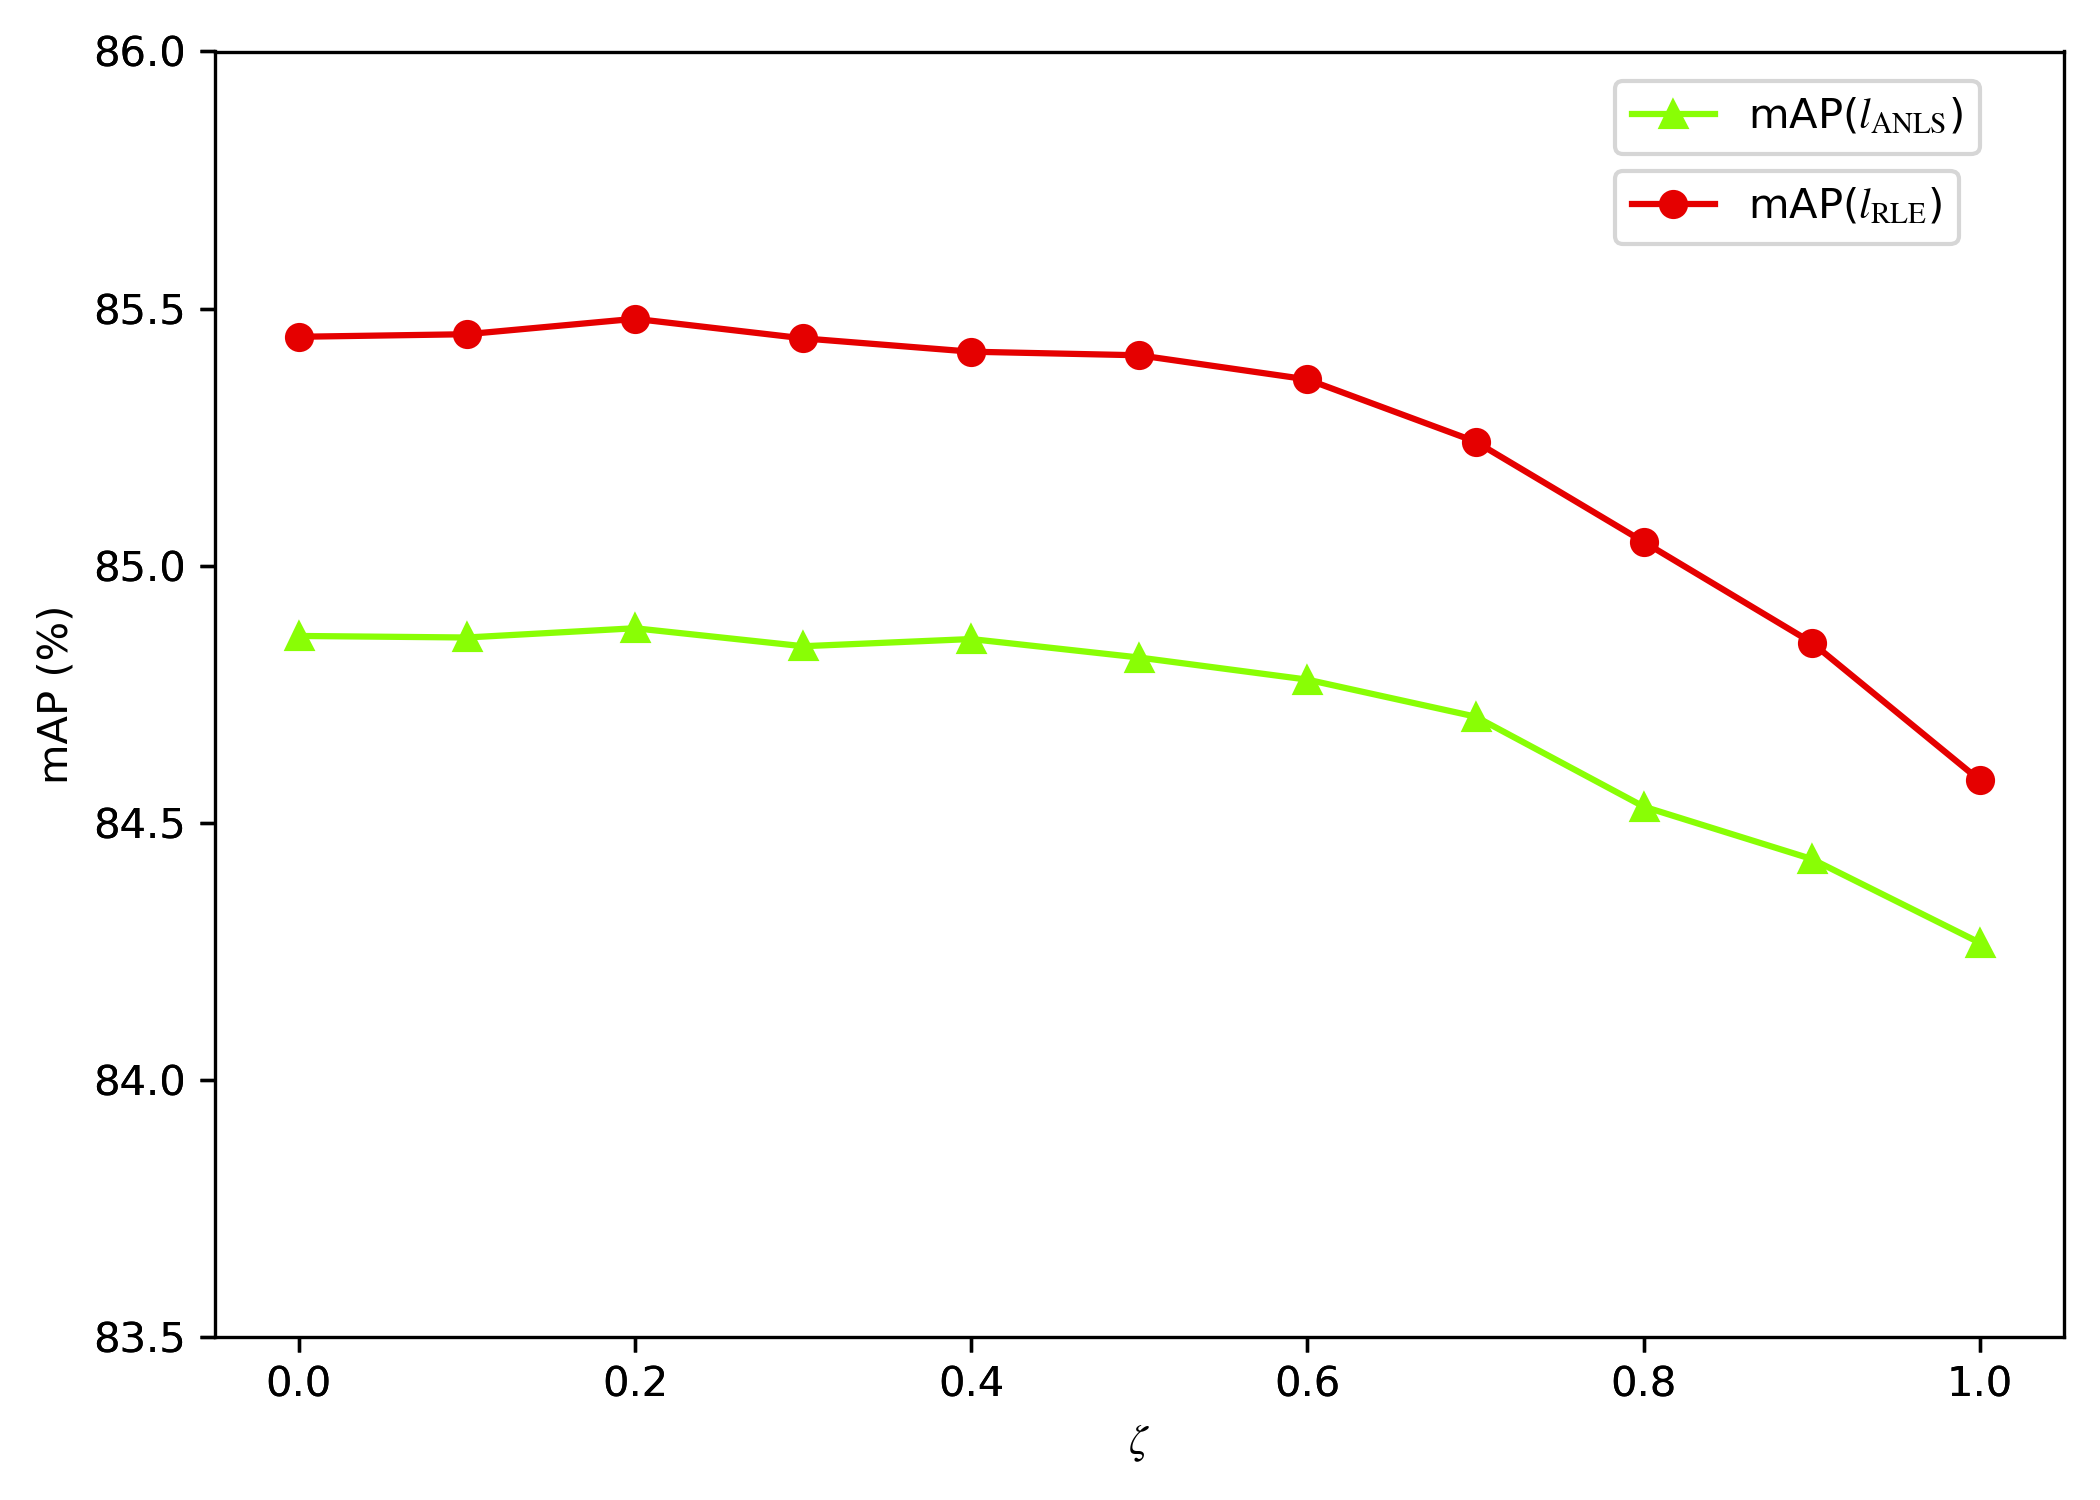
\includegraphics[width=0.7\linewidth]{char3_zeta_1.png}
    \caption{\label{fig3:zeta_1}在$Pascal~Voc$数据集上,LTR=60\%且$\sigma=1$时dSPUM算法基于不同损失函数在不同锚点阈值$\zeta$下的mAP值。}
\end{figure}
\begin{figure}[htbp]
    \centering
    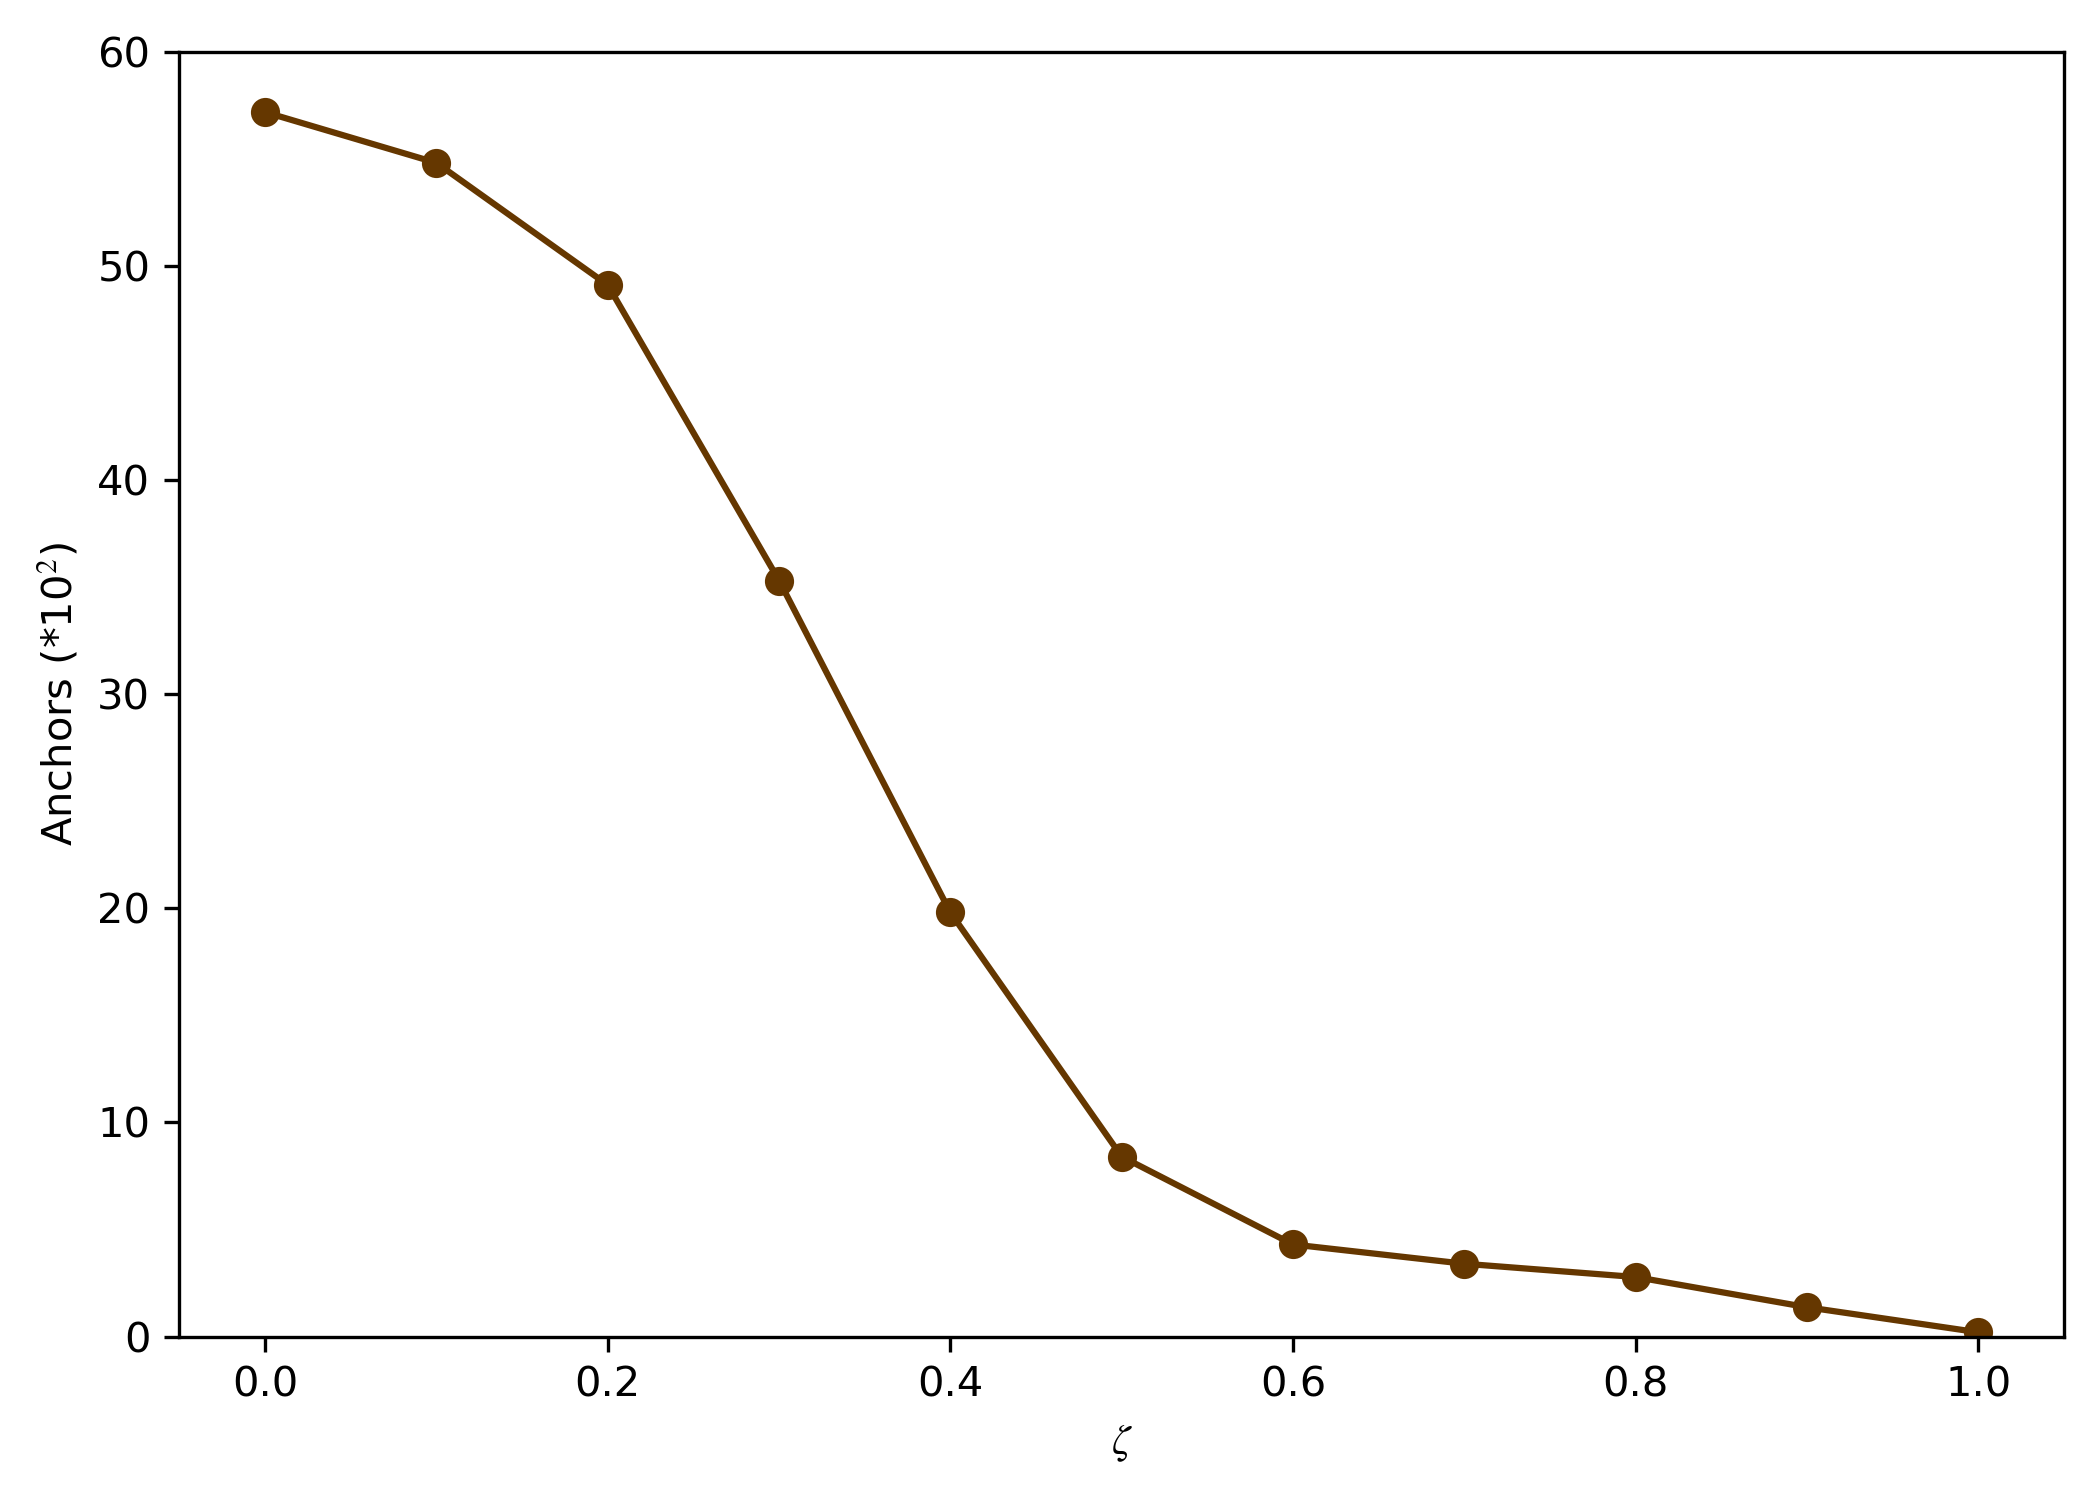
\includegraphics[width=0.7\linewidth]{char3_zeta_2.png}
    \caption{\label{fig3:zeta_2}{在$Pascal~Voc$数据集上,LTR=60\%且$\sigma=1$时dSPUM算法基于不同锚点阈值$\zeta$得到的平均锚点数据集大小。}}
\end{figure}
在$\mathrm{LTR=60\%}$的条件下,首先考虑锚点数据集阈值设置为$\zeta=0$、正标签数量期望值$k=4$,且事件触发阈值$\delta=0$即一直触发的情况,
对流形约束的比例参数$\sigma$进行范围在$\left\{0.01, 0.05, 0.1, 0.5, 1, 5, 10, 50, 100\right\}$的探索,
其结果如\autoref{fig3:sigma}所示,基于各损失函数的dSPUM算法都在$\sigma=1$附近时达到最佳mAP值,因此选取$\sigma=1$作为流形约束比例系数。
确定比例参数$\sigma=1$后,对锚点阈值$\zeta$进行值域为$\left[0,1\right]$且间隔为0.1的网格搜索。
结果如\autoref{fig3:zeta_1}和\autoref{fig3:zeta_2}所示,基于各损失函数的dSPUM算法基本在$\zeta=0.5$时mAP值上升趋于平缓,
因此基于网络通信代价考虑不再使用更小的$\zeta$值,将$\zeta=0.5$作为dSPUM算法在$Pascal~Voc$数据集上的最优设置。
由于锚点数据集的建立是基于数据相似度的,因此对于不同分布的数据集会存在不同的最佳阈值$\zeta$,需要单独设置。

\begin{figure}[htbp]
    \centering
    \includegraphics[width=0.7\linewidth]{Char3_k.png}
    \caption{\label{fig3:k}{在$Pascal~Voc$数据集上,LTR=60\%时dSPUM算法基于$l_{\mathrm{RLE}}$损失函数在不同正类标签数量期望值$k$下的mAP值。}}
\end{figure}

在其余条件不变的情况下,对正类数量约束的正标签数量期望值$k$进行探索,涉及到正类数量约束的损失函数仅有$l_{\mathrm{RLE}}$。
因此,对基于$l_{\mathrm{RLE}}$损失函数的dSPUM算法进行$k\in\left[0,L\right]$之间间隔为2的网格搜索,其中$L$为标签数目,在$Pascal~Voc$数据集中$L=20$。
其结果如\autoref{fig3:k},可以看出,随着$k$的变化,mAP值曲线的最高点出现在$k=4$处。因此对于$Pascal~Voc$数据集,正类数量约束中的正标签数量期望值$k$将被设置为4。
由于各数据集标签分布情况不同,因此对于不同分布的数据集会存在不同的最佳正标签数量期望值$k$,需要单独探索设置。

\begin{figure}[htbp]
    \centering
    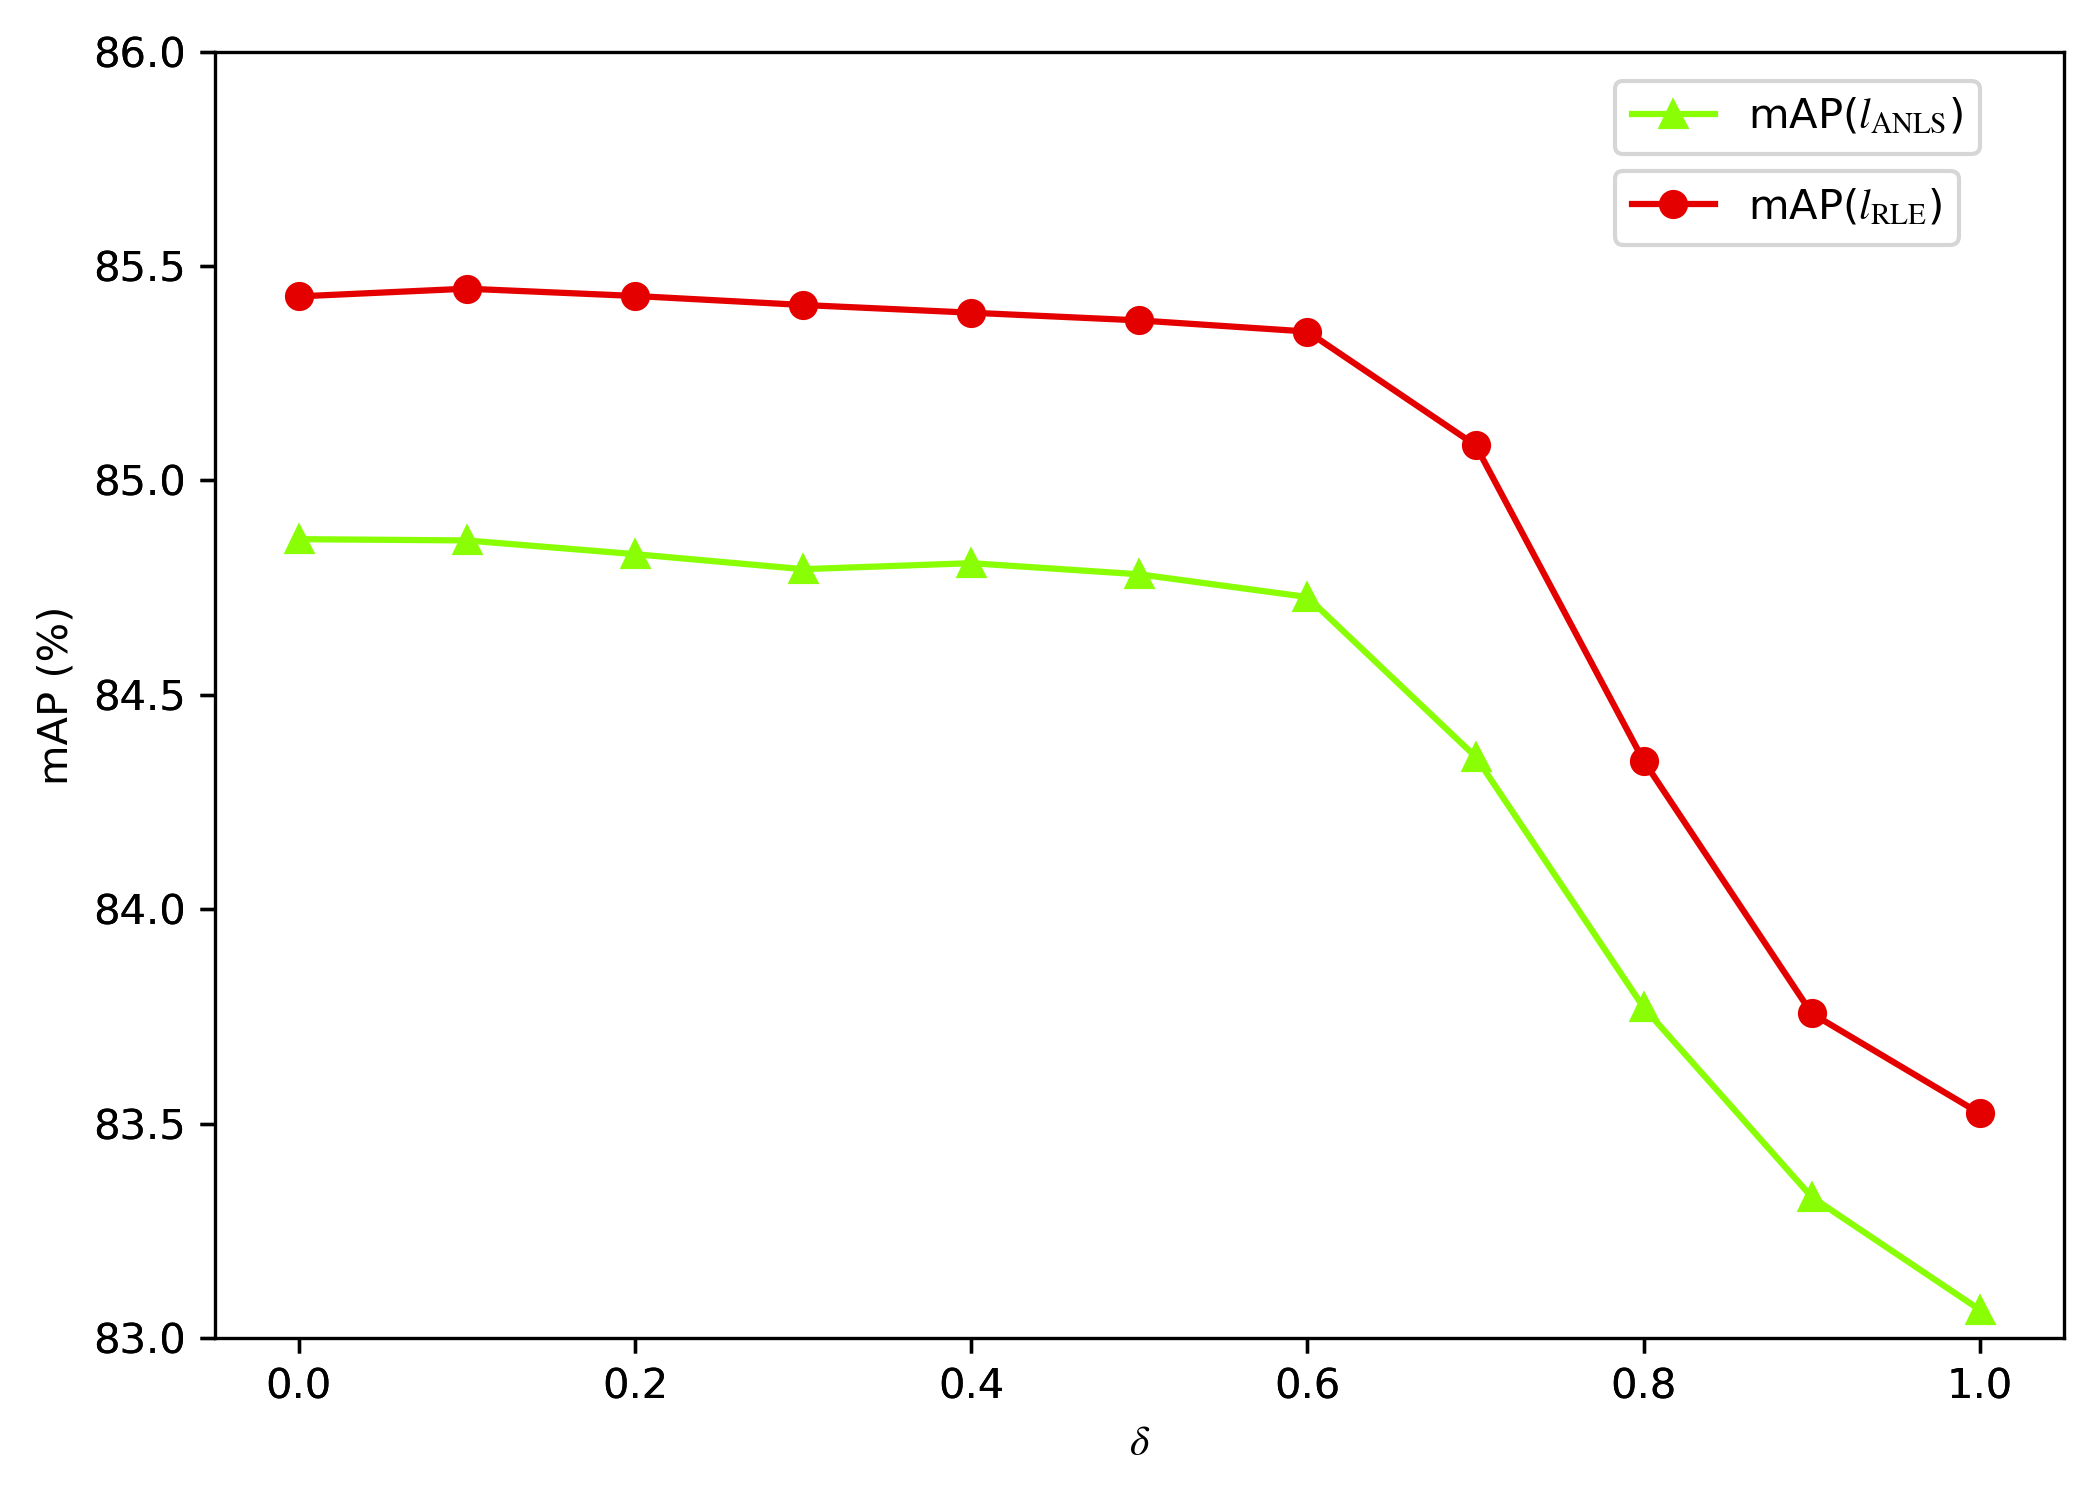
\includegraphics[width=0.7\linewidth]{char3_delta_1.png}
    \caption{\label{fig3:delta_1}{在$Pascal~Voc$数据集上,$\text{LTR=60\%}$时dSPUM算法在不同损失函数和事件触发阈值$\delta$下的mAP值。}}
\end{figure}
\begin{figure}[htbp]
    \centering
    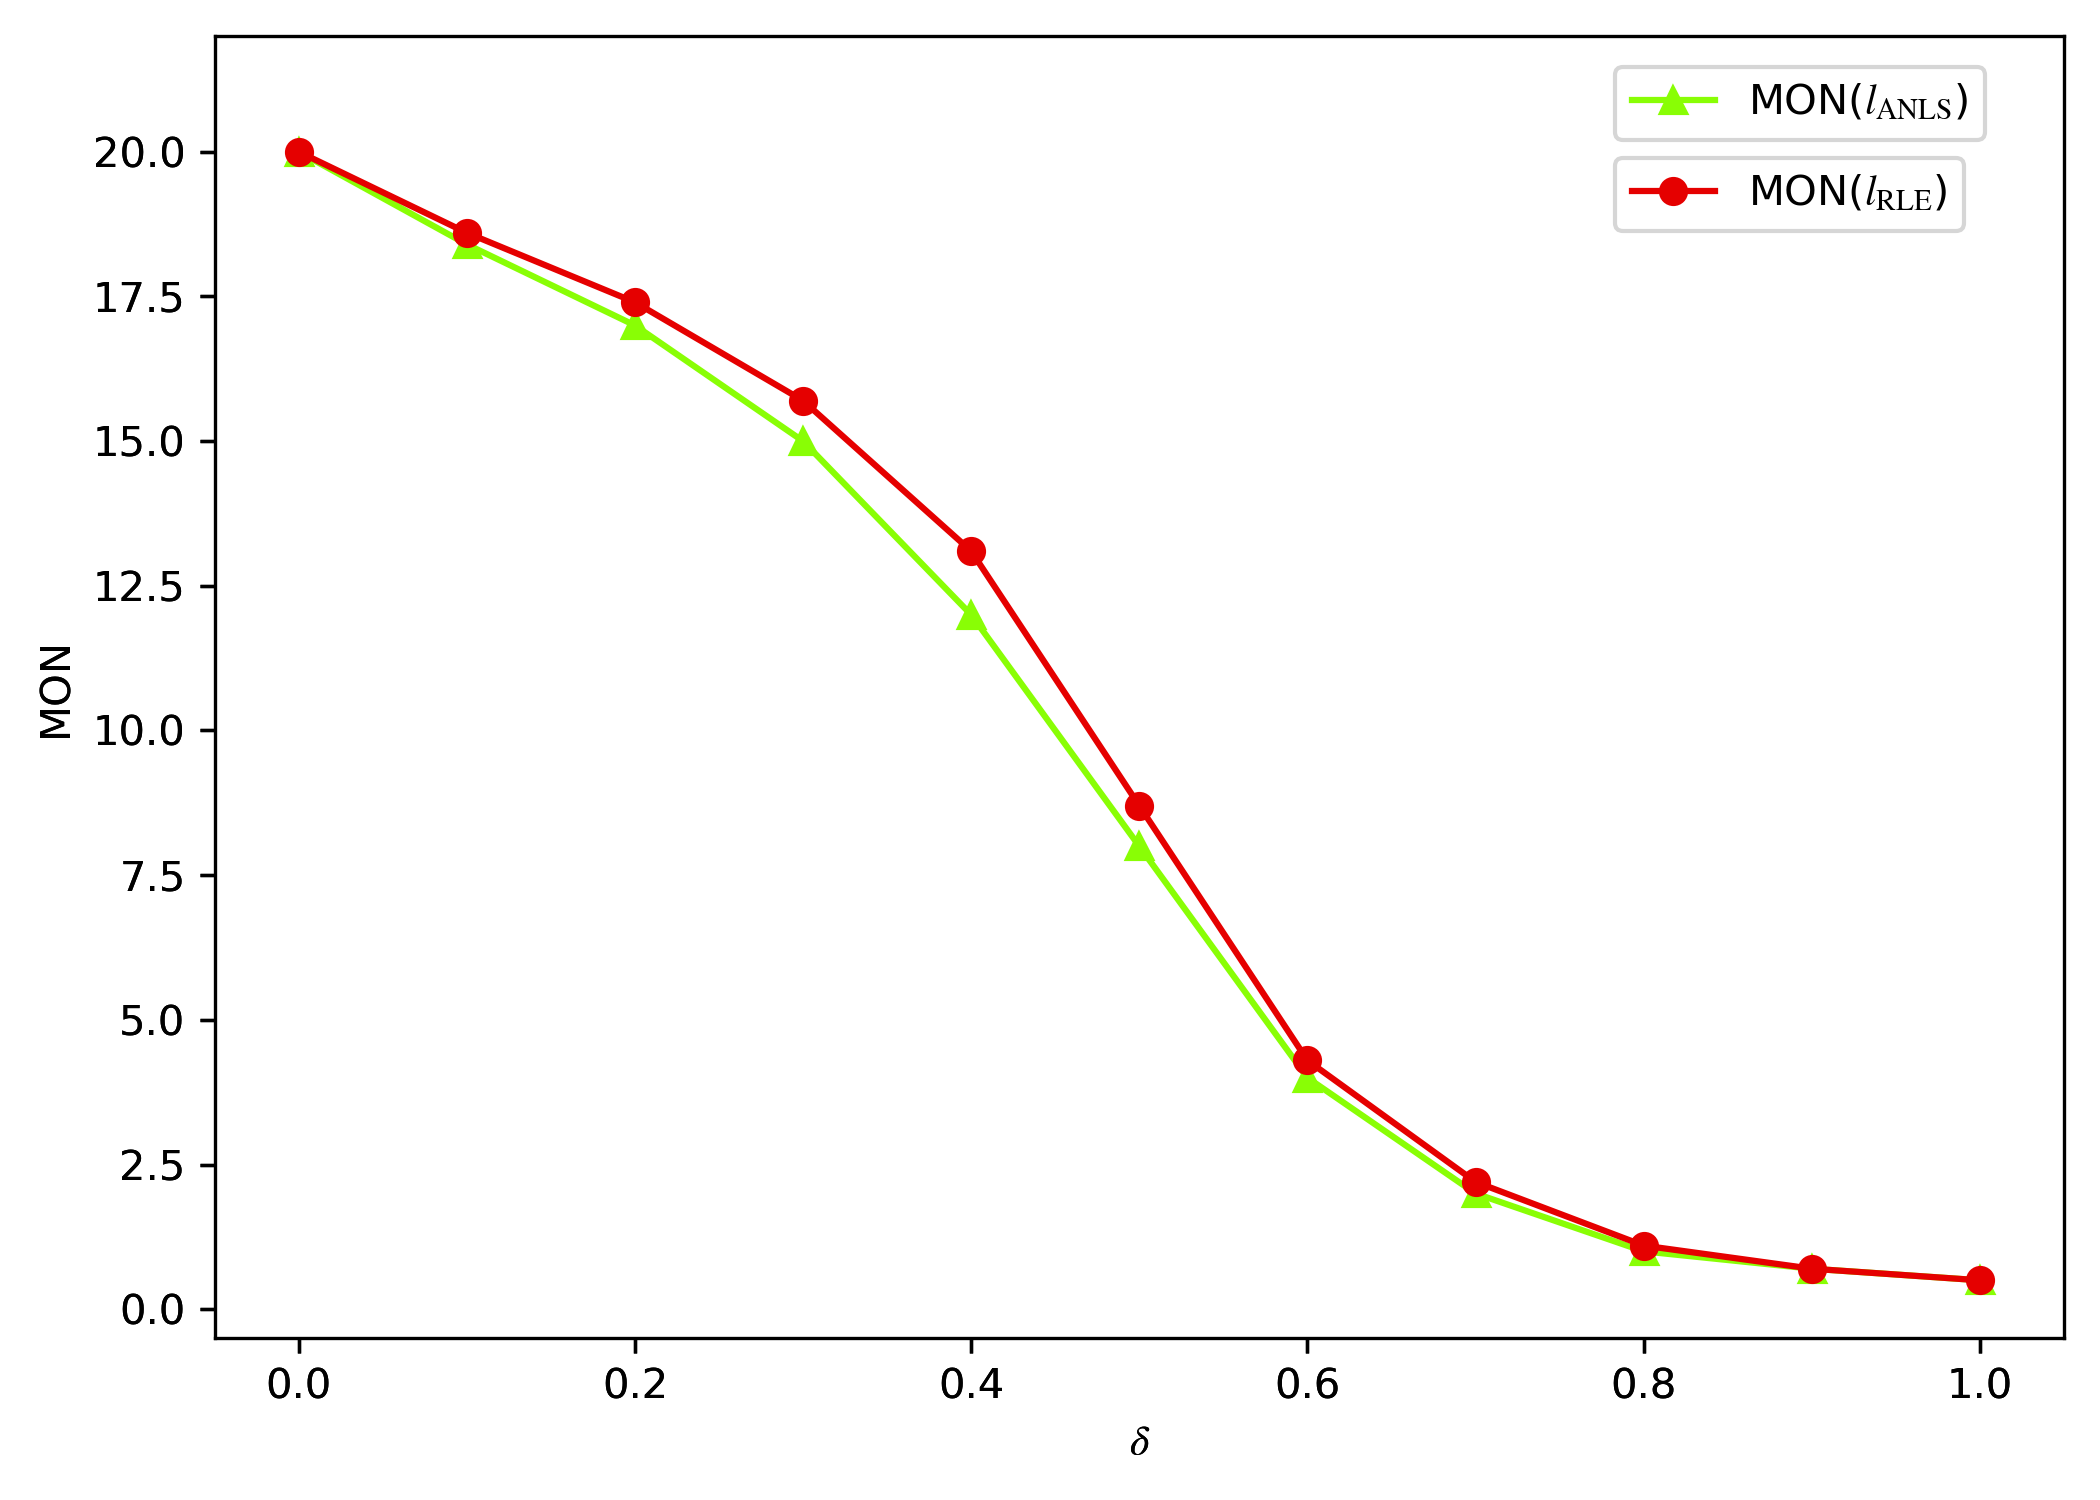
\includegraphics[width=0.7\linewidth]{char3_delta_2.png}
    \caption{\label{fig3:delta_2}{在$Pascal~Voc$数据集上,$\text{LTR=60\%}$时dSPUM算法在不同损失函数和事件触发阈值$\delta$下的事件触发频率MON。}}
\end{figure}
%然后对事件触发的设置进行探索。
在事件触发条件式\eqref{event_trigger}中,不同的阈值$\delta$会影响事件触发的频率,这种频率可用整个训练过程中
平均每次迭代中事件被触发的次数,即网络中与邻居节点进行信息传递的节点数量(mean open nodes,MON)来表示。
过大的$\delta$会导致事件触发困难进而影响分布式优化性能,而过小的$\delta$则会导致触发频率上升从而增加通信代价。
因此,本文在$\mathrm{LTR=60\%}$的条件下对$\delta$进行范围为$\left[0,1\right]$且间隔为0.1的网格搜索来探寻阈值
$\delta$的合适取值,其结果如\autoref{fig3:delta_1}和\autoref{fig3:delta_2}所示。
可以看到,对于本节提及的不同损失函数来说,其分类性能mAP皆在$\delta=0.6$上升趋势已基本趋于平缓,且若$\delta$继续下降
则MON会加速上升,这将会大大加剧网络的负担。
综合考虑性能与成本,在数据集$Pascal~Voc$上本文选择使用$\delta=0.6$作为事件触发的阈值,其余数据集上的阈值也将以相同方式进行确定。

\begin{figure}[htbp]
    \centering
    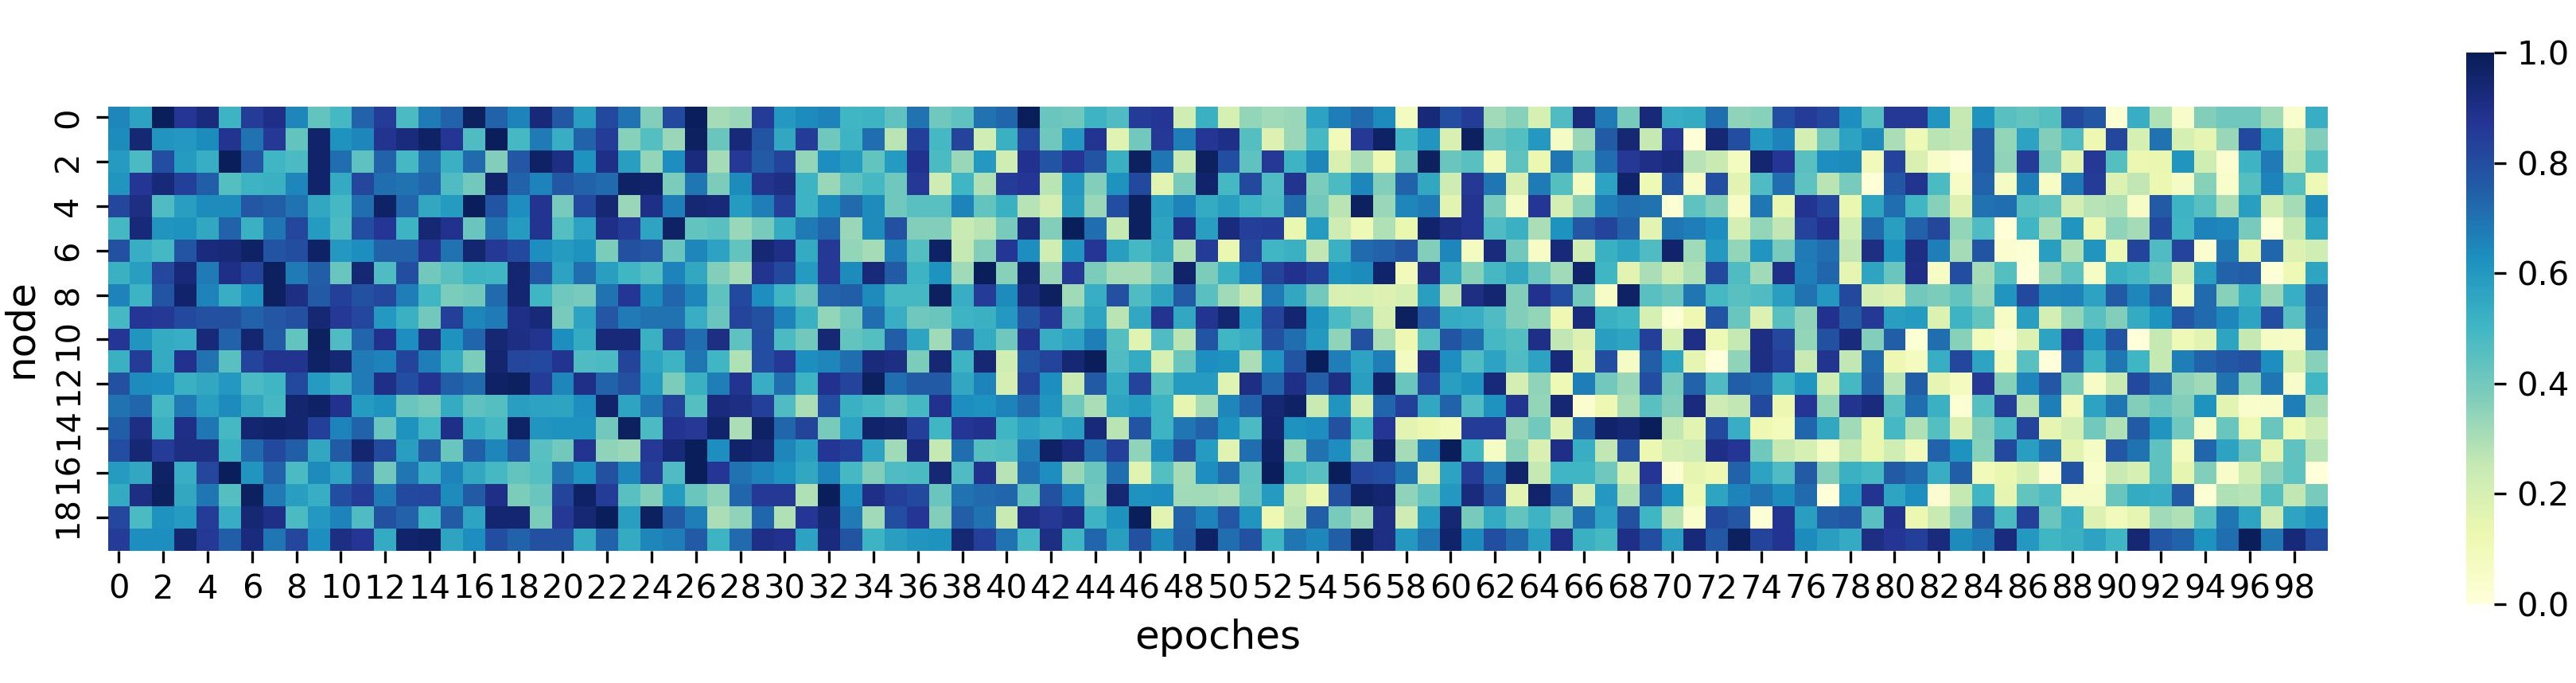
\includegraphics[width=1\linewidth]{Char3_events1.jpg}
    \caption{\label{fig3:events1}在$Pascal~Voc$数据集上,LTR=60\%且$\delta=0.6$的条件下dSPUM算法在训练轮数50-150时各节点
    $\boldsymbol\varPsi_j\left(t\right)$相比于$\boldsymbol\varPsi_j\left(t_j^{event}\right)$的变化率。}
\end{figure}
\begin{figure}[htbp]
    \centering
    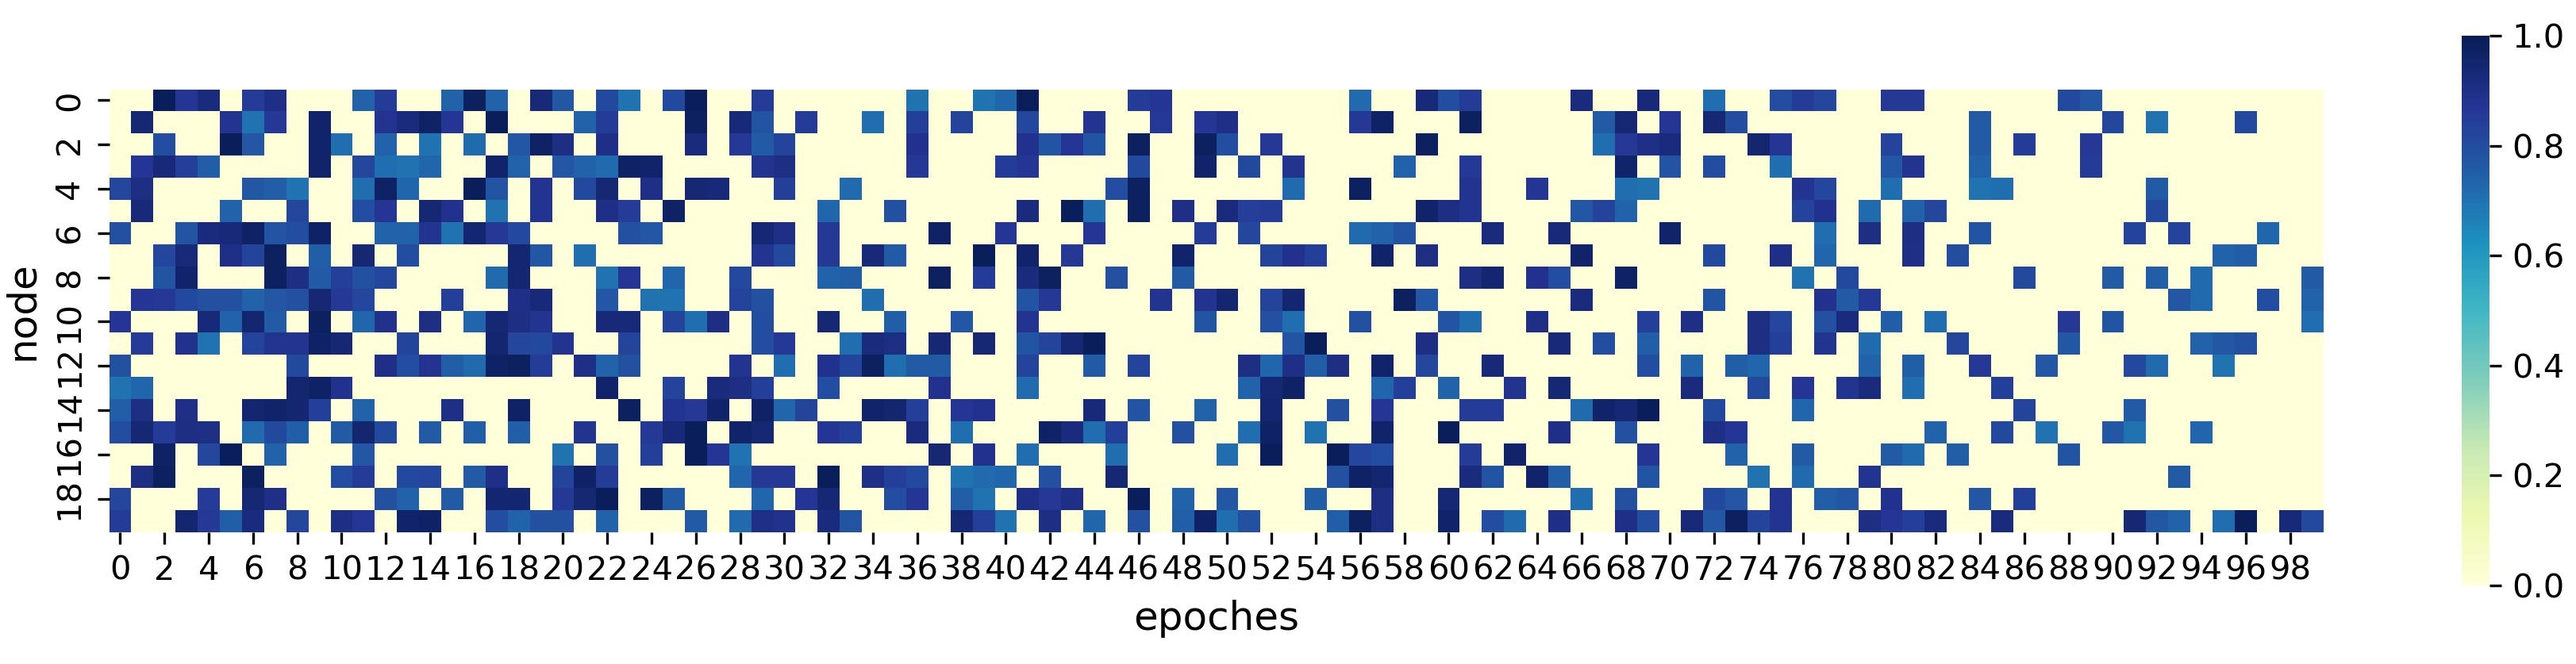
\includegraphics[width=1\linewidth]{Char3_events2.jpg}
    \caption{\label{fig3:events2}在$Pascal~Voc$数据集上,LTR=60\%且$\delta=0.6$的条件下dSPUM算法在训练轮数50-150时各节点
    事件的触发情况。}
\end{figure}
为了展示事件触发策略的效果,在$\mathrm{LTR=60\%}$且$\delta=0.6$的条件下使用损失函数$l_{\mathrm{RLE}}$,
截取训练轮数50-150时各节点$\boldsymbol\varPsi_j\left(t\right)$相比于$\boldsymbol\varPsi_j\left(t_j^{event}\right)$
的变化率情况以及各节点事件即式\eqref{event_trigger}触发的情况。 
\autoref{fig3:events1}展示了随着迭代轮数的增加,各节点$\boldsymbol\varPsi_j\left(t\right)$的变化率情况。\autoref{fig3:events2}则展示了在事件触发阈值$\delta=0.6$的情况下,各节点满足事件即式\eqref{event_trigger}的触发情况。
从图中可以得到,随着训练轮数的增加,事件被触发即需要传递信息的节点数量会逐渐减少,这大大减轻了整个网络的传输负担,证实了事件触发算法的优越性。

\begin{figure}[htbp]
    \centering
    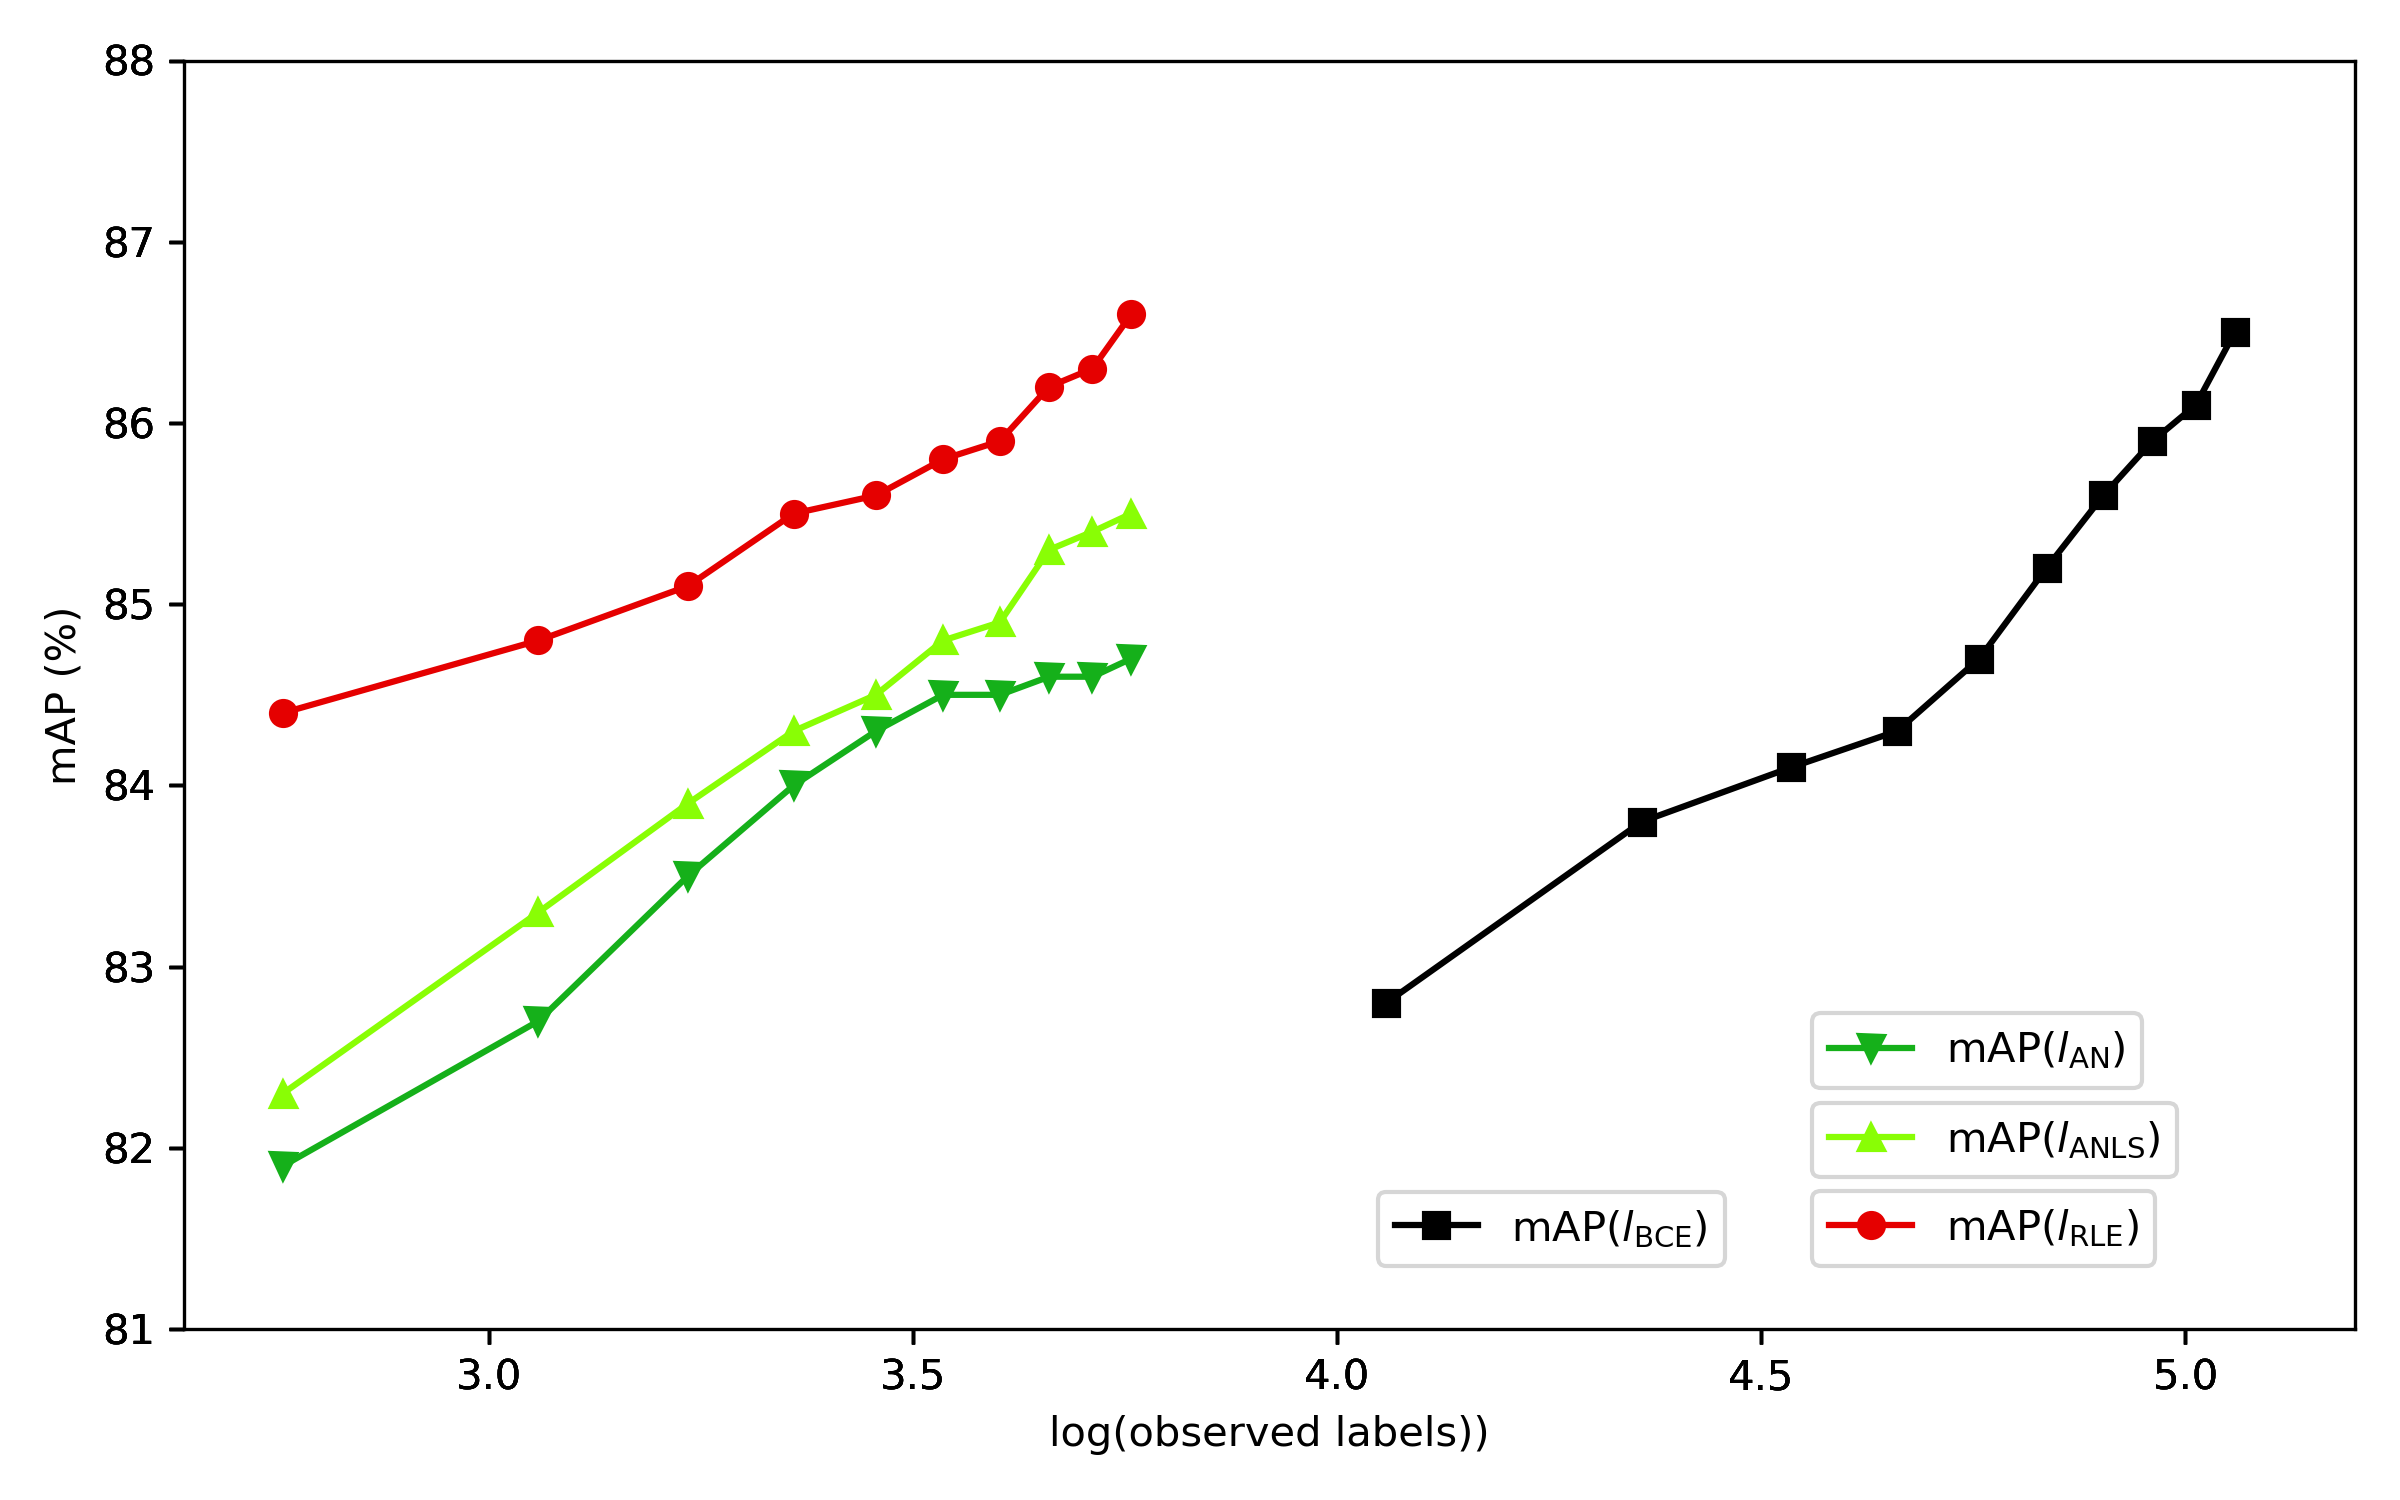
\includegraphics[width=0.8\linewidth]{char3_mAP_losses.png}
    \caption{\label{fig3:mAP}{在$Pascal~Voc$数据集上,在不同观测标签数量下dSPUM算法基于不同损失函数的mAP值。}}
\end{figure}
在上述参数设置条件下,对基于不同损失函数的dSPUM算法在$\left[0,1\right]$范围内进行间隔为0.1的不同LTR的性能对比。
同时作为对比,本文的仿真仍对需要完整的$L$个标签的$l_{\mathrm{BCE}}$损失函数在完整标注的$Pascal~Voc$数据集上进行了性能测试,
且其在不同PTR条件下仅针对标注数据$\mathcal{N}^l$计算$l_{\mathrm{BCE}}$损失函数并优化。
实验结果如\autoref{fig3:mAP}所示,其横坐标为整个训练数据集中可用的观测标签数量(observed labels),除$l_{BCE}$为$\mathrm{LTR}*20*N$外,其余各损失函数可用正观测标签数量为$\mathrm{LTR}*N$。
从图中可以看出,相比于所需全部标签的$l_{\mathrm{BCE}}$来说,本节提出的半监督单正例损失函数$l_{\mathrm{ANLS}}$和$l_{\mathrm{RLE}}$
仅需要极少的观测标签数量即可得到与其接近的分类性能。

\begin{table}[htbp]
    \caption{\label{char3:tab:data_description}数据描述}
    \begin{tabularx}{\textwidth}{XXXXXXX}
        \hline
        数据集 & 训练集大小$~~$ & 测试集大小$~~$ & 标签数量 & $\zeta$ & $k$ & $\delta$\\ \hline
        VOC & 5717 & 5823 & 20 &  0.5 & 4 & 0.6\\
        COCO & 82081 & 40137 & 80 &  0.5 & 2 & 0.5\\
        NUS & 123034 & 82234  & 81 & 0.3 & 6 & 0.5\\
        CUB & 5994 & 5794 & 312 &  0.7 & 40 & 0.4\\
        DOTA & 2306 & 500 & 14 &  0.5 & 4 & 0.5\\ 
        UD & 82082 & 56167 & 8 &  0.6 & 2 & 0.3\\ \hline
    \end{tabularx}
\end{table}

\begin{table}[htbp]
    \caption{\label{char3:tab:mAPs}不同算法在各数据集上基于不同LTR的性能(mAP)比较}
    \begin{tabularx}{\textwidth}{XXXXXXX}
        \hline
        \multirow{2}*{数据集} & \multirow{2}*{LTR(\%)} & \multicolumn{5}{c}{mAP(\%)}\\
        \cline{3-7}
        \multicolumn{1}{c}{} & & BP-MLL & MLkNN-LS & SDRL & dSPUM-$l_\mathrm{ANLS}$ & dSPUM-$l_\mathrm{RLE}$\\
        \hline
        \multirow{3}*{VOC} 
        & 10.0 & 79.1$\pm$1.1 & 78.9$\pm$1.1 & 82.4$\pm$0.3 & 82.3$\pm$0.9 & \textbf{84.4$\pm$0.3} \\
        & 30.0 & 81.3$\pm$1.2 & 80.7$\pm$1.1 & 83.5$\pm$0.5 & 83.9$\pm$0.4 & \textbf{85.1$\pm$0.4} \\
        & 60.0 & 82.4$\pm$1.9 & 82.3$\pm$0.7 & 84.1$\pm$0.1 & 84.8$\pm$0.4 & \textbf{85.8$\pm$0.2} \\ \hline

        \multirow{3}*{COCO} 
        & 10.0 & 59.1$\pm$1.2 & 53.6$\pm$1.3 & 62.8$\pm$0.3 & 61.4$\pm$0.8 & \textbf{63.9$\pm$0.7} \\
        & 30.0 & 60.8$\pm$1.1 & 59.2$\pm$1.2 & 63.1$\pm$0.7 & 63.3$\pm$0.2 & \textbf{64.7$\pm$0.7} \\
        & 60.0 & 62.9$\pm$1.4 & 61.2$\pm$1.2 & 63.7$\pm$0.4 & 64.3$\pm$0.4 & \textbf{65.2$\pm$0.4} \\   \hline
        
        \multirow{3}*{NUS} 
        & 10.0 & 48.3$\pm$0.9 & 47.0$\pm$0.3 & 49.1$\pm$0.6 & 51.0$\pm$0.6 & \textbf{51.5$\pm$0.4} \\ 
        & 30.0 & 49.3$\pm$0.8 & 48.7$\pm$0.1 & 50.0$\pm$1.5 & 51.7$\pm$0.3 & \textbf{52.9$\pm$0.5} \\
        & 60.0 & 50.1$\pm$0.9 & 49.1$\pm$0.9 & 50.8$\pm$0.5 & 52.4$\pm$0.5 & \textbf{53.0$\pm$0.3} \\    \hline

        \multirow{3}*{CUB} 
        & 10.0 & 11.9$\pm$0.8 & 12.0$\pm$0.3 & 13.2$\pm$0.6 & \textbf{14.6$\pm$0.3} & 14.5$\pm$0.4 \\ 
        & 30.0 & 12.9$\pm$0.3 & 12.7$\pm$0.5 & 13.7$\pm$1.5 & 14.9$\pm$0.3 & \textbf{15.3$\pm$0.6} \\
        & 60.0 & 12.9$\pm$0.7 & 13.1$\pm$0.1 & 14.3$\pm$0.5 & 15.4$\pm$0.1 & \textbf{16.0$\pm$0.3} \\    \hline
        
        \multirow{3}*{DOTA} 
        & 10.0 & 72.4$\pm$0.4 & 68.4$\pm$0.3 & 75.3$\pm$1.2 & \textbf{76.1$\pm$0.9} & 75.5$\pm$0.4 \\ 
        & 30.0 & 75.7$\pm$0.2 & 69.7$\pm$0.3 & 76.4$\pm$1.1 & \textbf{76.7$\pm$0.5} & 76.3$\pm$0.4 \\
        & 60.0 & 76.0$\pm$0.6 & 70.1$\pm$0.5 & \textbf{77.3$\pm$1.5} & 76.9$\pm$0.1 & 77.2$\pm$0.3 \\   \hline
        
        \multirow{3}*{UD} 
        & 10.0 & 82.1$\pm$1.2 & 80.6$\pm$1.3 & 82.2$\pm$1.2 & 84.3$\pm$0.9 & \textbf{84.5$\pm$0.8} \\   
        & 30.0 & 83.1$\pm$0.9 & 83.0$\pm$0.3 & 83.1$\pm$1.1 & 84.6$\pm$0.2 & \textbf{84.7$\pm$0.2} \\
        & 60.0 & 83.3$\pm$0.7 & 83.6$\pm$0.1 & 84.3$\pm$1.0 & \textbf{85.2$\pm$0.7} & 85.1$\pm$0.1 \\     \hline
        
        平均排名 & & 4.17 & 4.83 & 2.78 & 1.94 & \textbf{1.28} \\        \hline
    \end{tabularx}
\end{table}
\subsection{性能比较}
为了展示所提dSPUM算法的优越性能,本节将在不同LTR设置下在不同数据集上对比不同算法的分类性能。
由于本文提出的dSPUM算法基于部分数据中的单个正例标签被标注的SPUM数据,难以寻找基于相同标签设置的算法进行对比。
因此本文对比了基于单个标签的多标签学习算法,标签反向传播(Backpropagation for Multi-Label Learning,BP-MLL)算法\cite{Adikhresna_BPMLL_2020},并在不同PTR条件下仅使用标注数据进行训练;
同时,本文还对比了两种半监督多标签学习算法,基于标签传播的多标签k近邻(Multi-label k-Nearest Neighbors with Label Spead, MLkNN-LS)
算法\cite{Lucena_Semi_2016}和半监督对偶关系学习(Semi-supervised Dual Relation Learning,SDRL)算法
\cite{Wang_Semi_2021},并在标注数据中用“假负”策略即仅使用一个被选中的正例标签并将其余未标注标签设置为负进行训练。

由于多标签数据在真实世界中最常见于目标检测任务,因此本文主要使用一些常用的目标检测数据集,
其中有$Pascal~~Voc~~2012\left(VOC\right)$,$Microsoft~~COCO~~2014\left(COCO\right)$,
$NUS-WIDE\left(NUS\right)$,$CUB-200-2011\left(CUB\right)$,$DOTA$和$UA-DETRA\left(U-D\right)$。
将各数据集根据不同PTR条件分为一部分单正例标注数据(标签向量中随机选取一个正例标签选入观测标签$+1$,其余都置为$\varnothing$)和一部分未标注数据,以构造SPUM数据集。
在参数设置上基于以上实验将流形约束比例参数$\sigma$设置为1,
而各数据集的锚点阈值$\zeta$、正标签数量期望值$k$和事件触发门限$\delta$
则将分别探索设置最优值,并与数据集的介绍共同展示在\autoref{char3:tab:data_description}中。
本文在实验中先对训练数据集随机分为10份进行十折交叉验证(ten-fold validation),
选取在验证集上表现最好的参数来对测试集进行分类,共进行50次上述实验得到测试集分类效果mAP均值和方差。

本文将基于损失函数$l_{\mathrm{ANLS}}$和$l_{\mathrm{RLE}}$的dSPUM算法分别记为
$\mathrm{dSPUM}-l_{\mathrm{ANLS}}$和$\mathrm{dSPUM}-l_{\mathrm{RLE}}$
,各算法在不同数据的不同LTR条件下的表现如\autoref{char3:tab:mAPs}所示,其中粗体表示算法在该数据集的特定LTR条件下根据mAP值排名第一。
从实验结果可以看到相比于其他算法,$\mathrm{dSPUM}-l_{\mathrm{RLE}}$和$\mathrm{dSPUM}-l_{\mathrm{ANLS}}$在不同的LTR条件下平均排名分别位列第一、第二。
为了验证dSPUM算法的优越性,本文使用多标签领域常用的弗得里曼检验(Friedman test)来进行差异性验证,弗得里曼统计量$F_F$计算方法如下:
\begin{equation}
    \label{Friedman test}
    F_F = \frac{\left(M-1\right)\kappa_F^2 }{M\left(I-1\right)-\kappa_F^2},~
    \kappa_F^2=\frac{12M}{I\left(I+1\right)}\left[\sum_{\iota=1}^IR_\iota^2 - \frac{I\left(I+1\right)^2}{4}\right],
\end{equation}
其中$M$表示数据集的数量,$I$表示算法的数量,$R_\iota^2$表示第$\iota$个算法在$M$个数据集上的平均排名。
根据每一种算法在6个数据集上的mAP平均排名,可以计算出在算法总数$I=5$,数据集总数$M=6$情况下的弗得里曼统计量$F_F=38.54$,
其大于置信度$\alpha=0.05$下的临界值$CD=F_{\alpha}\left(I-1,M-1\right)=5.19$,其中$F_{\alpha}\left(I-1,M-1\right)$为自由度为$I-1$和$M-1$的
F分布。
由此,我们可以否定零假设,说明上述五种算法确实存在性能上的明显差异。

此外,本文使用后续布氏检验(Bonferroni-Dunn test)来进行后续验证dSPUM算法是否显著优于其他算法。
{布氏检验的临界值$CD$计算方式如下:
\begin{equation}
    \label{Bonferroni-Dunn test}
    CD = q_\alpha\sqrt{\frac{I\left(I+1\right)}{6M}},
\end{equation}
其中$M$表示数据集的数量,$I$表示算法的数量,$q_\alpha$可查表获得。在算法总数$I=5$、数据集总数$M=6$}且置信度$\alpha=0.05$的情况下,布氏检验的临界值$CD=2.28$。如\autoref{fig3:BDtest}所示,我们将$\mathrm{dSPUM}-l_{\mathrm{RLE}}$作为控制算法,与其{平均排名}相差小于布氏检验的临界值$CD$的算法将会用红线标注出来。
\begin{figure}
    \centering
    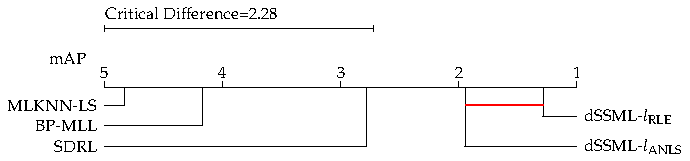
\includegraphics[width=1\linewidth]{char3_BDtest.pdf}
    \caption{\label{fig3:BDtest}对不同算法进行Bonferroni-Dunn统计检验的结果。}
\end{figure}
从图中可以看出,本文所提出的$\mathrm{dSPUM}-l_{\mathrm{RLE}}$算法排名第一,且除了与本文提出的$\mathrm{dSPUM}-l_{\mathrm{ANLS}}$算法性能相近外,
与其余现有同类算法有着明显的性能差异,证明本文所提出的$\mathrm{dSPUM}$从未观测标签和未标注数据中学到了有效信息。

% Chapter 3.5
\section{本章小结}\label{Char3_Summary}
本节针对多标签分类中仅有部分数据的单个正例被观测到的单正例无标注多标签学习场景,提出了一系列可从SPUM数据中学习信息的损失函数。
然后对各节点设计去中心化损失函数并提出全局优化问题,且引用了基于锚点数据的流形正则化。
对全局优化问题使用分布式梯度下降进行优化,并使用了事件触发机制来减少节点间传递信息的频率以降低网络负担。
此外,本文对单一数据集使用网格搜索进行了最优参数设置的探索,然后对比一些前沿的相似算法在多个数据集上进行了仿真实验,最终通过
弗得里曼检验(Friedman test)及其后续检验布氏检验(Bonferroni-Dunn test)验证了本文提出的dSPUM算法的优越性能。

% Chapter 4
\chapter{基于最坏扰动的分布式优化}
\section{引言}
由于深度学习通常使用规模较大、层数较深的神经网络框架,其极易专注于学习训练集所代表的小领域而在实际复杂环境数据中表现较差,这一点在标注数据较少的半监督情况下尤为突出。因此,探索预防过拟合的方法是在深度学习中一个至关重要的领域。为了有效解决这一问题,人们提出了许多方法。最经典的解决方法是搜集范围更广的人工标注数据集,这显然有悖于半监督领域期望使用少量标注数据获得较好学习效果的初衷\cite{Shorten_DataAugmentation_2019}。此外,随机参数扰动和随机连接扰动(如dropout\cite{Wei_Dropout_2020})也是较常使用的预防过拟合的方法,它可以通过对框架的干扰使得算法即使在{极端情况}下也能得到一个较好的输出,从而使算法的输出在不同环境中都具有较好的鲁棒性。但上述扰动过于随机,无法对理论结果进行较好的分析。在本章,将通过计算探索对于神经网络来说最坏的扰动,其可以最大程度地对网络进行破坏,从而使得算法获得最大程度的鲁棒性以增强对未见数据的分类性能\cite{Zhang_WCP_2020}。

在本章中,考虑可对神经网络影响最大的、最坏扰动并将其拓展到分布式场景,对上文提出的dPU和dSPUM算法的性能进行优化。本章余下部分的简介如下:
在\ref{Char4_Preliminaries}节,简要介绍了一些预备知识如随机噪声扰动和随机连接扰动。
在\ref{Char4_LossDesign}节,描述了能够最大程度破坏神经网络的最坏扰动。
在\ref{Char4_Distributed}节,将最坏扰动推广到分布式场景,使用锚点数据集实现全局最坏扰动。
在\ref{Char4_Experiments}节,利用若干真实数据集测试了对dPU和dSPUM算法施加以最坏扰动的效果,
充分比对证实了最坏扰动算法的优越性。
在\ref{Char4_Summary}节,对本章的工作做出了总结。

\section{问题描述与预备知识}\label{Char4_Preliminaries}
网络扰动主要是对构成算法的基本框架(如各式神经网络)进行随机地破坏,迫使算法在模型参数遭到破坏而产生较大幅度偏转时也能较好地进行预测。相应地,即使在{数据分布偏差较大的未见离群值}输入时也能有较好的性能。常见扰动算法主要有随机噪声扰动和随机连接扰动。随机噪声扰动是对算法的参数如$\boldsymbol\theta$施加以随机噪声,如:
\begin{equation}
    \label{P1}
    \boldsymbol\theta^p = \boldsymbol\theta + \boldsymbol\vartheta,
\end{equation}
其中$\boldsymbol\theta^p$为扰动后的参数,$\boldsymbol\vartheta$为扰动噪声并通常由高斯随机分布得到。

dropout则是另外一种著名的参数扰动策略,其通过以相应的比例随机切断层间的连接以达到约束最坏情况下输出的隐式正则化效果\cite{Wei_Dropout_2020}。如\autoref{Char1:fig:dropout}所示,其中虚线代表着即将被切断的层间连接,可见算法的结构被一定程度地破坏了。
若是在被随机噪声干扰或随机连接切断过的网络上仍能做到良好的分类性能,那么算法将会更具鲁棒性\cite{Krizhevsky_ImageNet_2012}。
\begin{figure}[htbp]
    \centering
    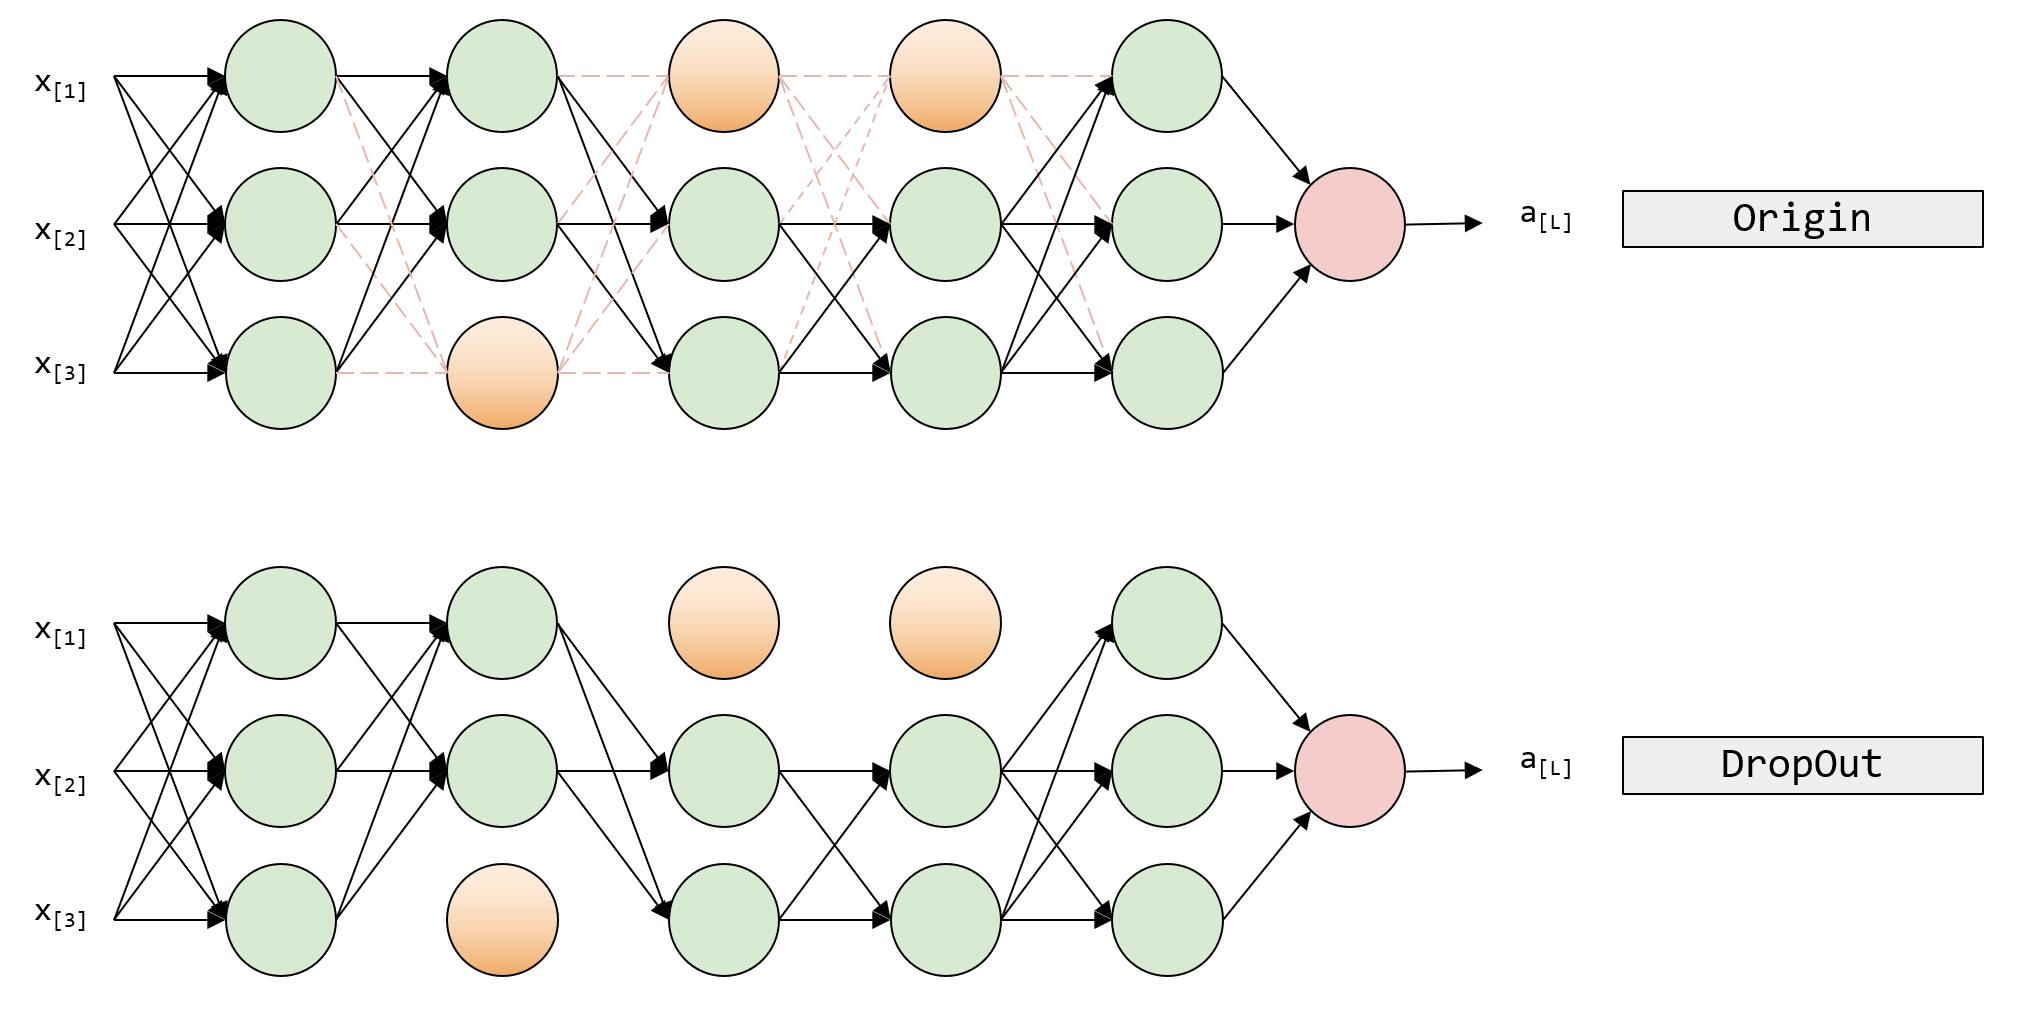
\includegraphics[width=0.9\linewidth]{Char1/dropout.jpg}
    \caption{\label{Char1:fig:dropout}{一个经过dropout扰动的神经网络。}}
\end{figure}

这一章我们将通过对用于提取特征的神经网络{施加}一种扰动优化策略,进一步提升半监督算法的性能。与dSPUM算法一样,dPU算法在本章也将与一个神经网络框架ResNet50的特征层进行连接并一起训练。与第二章和第三章所述不同的是,ResNet50的参数也将会加入其算法的模型参数(如$\boldsymbol\theta$和$\boldsymbol \varphi$)中,并以$\mathrm{dSPUM}-{l_{\mathrm{RLE}}}$为例算法结构将如\autoref{char4:fig:arc3}所示。
\begin{figure}
    \centering
    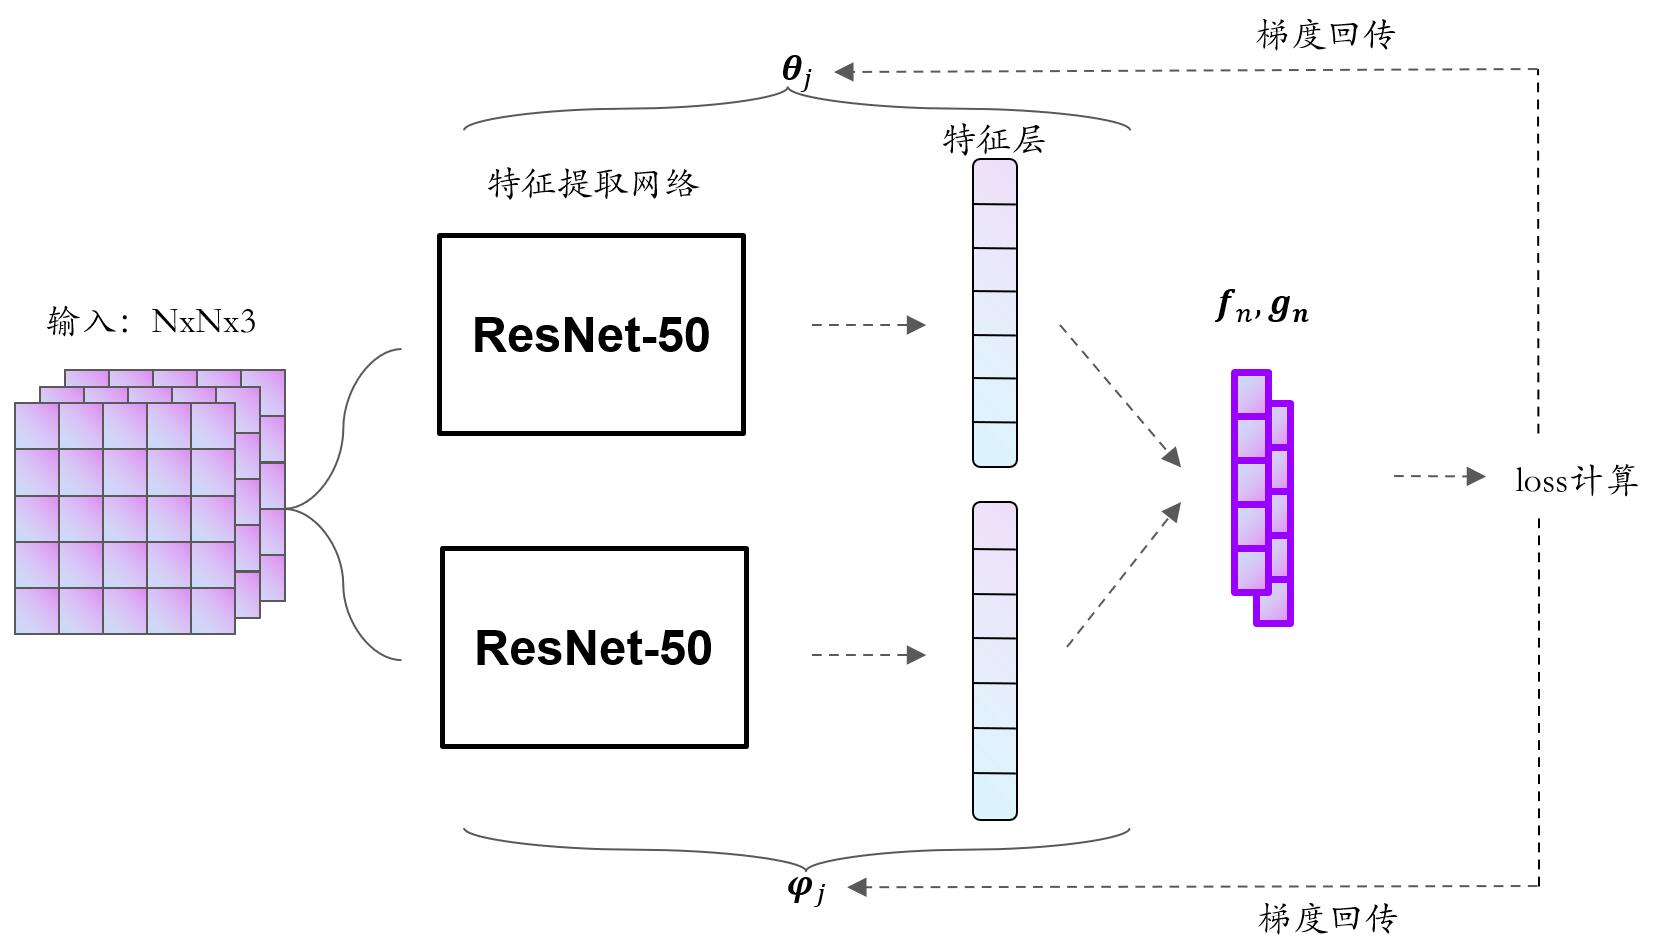
\includegraphics[width=1\linewidth]{char4_arc3_role_total.jpg}
    \caption{\label{char4:fig:arc3}{将ResNet50的参数也加入优化的
    $\mathrm{dSPUM}-{l_{\mathrm{RLE}}}$算法损失函数计算框架。}}
\end{figure}

% Chapter 4.2
\section{最坏扰动分析}\label{Char4_LossDesign}
最坏扰动是指在模型参数$\boldsymbol\theta$的基础上进行一种数值上或者结构上的扰动得到扰动参数$\boldsymbol\theta^p$,
{其目的是寻找到使得$\boldsymbol f\left(\boldsymbol\theta^p,\boldsymbol x_n\right)$和
$\boldsymbol f\left(\boldsymbol\theta,\boldsymbol x_n\right)$的差别尽可能大的最坏扰动参数$\boldsymbol\theta^p$。}
则最大扰动约束项可用公式表示为:
\begin{equation}
    \label{Pertur_Re}
    \Omega_{\boldsymbol\theta}=\max _{\boldsymbol\theta^p \in \mathcal{P}}  \frac{1}{N} \sum_{n \in \mathcal{N}}
    \hslash\left(\boldsymbol f\left(\boldsymbol\theta,\boldsymbol x_n\right),
    \boldsymbol f\left(\boldsymbol\theta^p,\boldsymbol x_n\right)\right)
\end{equation}
其中$\mathcal{P}$是指对于扰动参数$\boldsymbol\theta^p$的约束范围,不同类型扰动的约束范围将在下文提及。
$\hslash$是衡量扰动输出与原始输出不同程度的差别函数,{本文使用L2损失函数作为差别函数}。

由式\eqref{Pertur_Re}学习到使得全局$\hslash$最大的最坏扰动参数后,$\Omega_{\theta}$可作为约束项被加入到原始损失函数中,
再对算法进行学习,即:
\begin{equation}
    \label{Loss_Pertur_Re}
    \min _{\boldsymbol\theta} 
    \frac{1}{N} \sum_{n \in \mathcal{N}}l(\boldsymbol f\left(\boldsymbol\theta,\boldsymbol x_n\right), \boldsymbol{z}_n)
    +\gamma \Omega_{\boldsymbol\theta}
\end{equation}
其中$l(\boldsymbol f\left(\boldsymbol\theta,\boldsymbol x_n\right), \boldsymbol{z}_n)$可更换为第二章和第三章提到过的任意正例无标注损失函数。

对于可加性扰动来说,其扰动参数$\boldsymbol\theta^p$可记为$\boldsymbol\theta^{p+}=\boldsymbol\theta+\boldsymbol\vartheta $,
其中$\boldsymbol\vartheta$为加性扰动。为了表示方便,
记$\boldsymbol f\left(\boldsymbol\theta,\boldsymbol x_n\right)$为$\boldsymbol f_n$,
$\boldsymbol f\left(\boldsymbol\theta^{p+},\boldsymbol x_n\right)$为$\boldsymbol f_n^{p+}$。
对差别函数$\hslash\left(\boldsymbol f_n,\boldsymbol f_n^{p+}\right)$进行在$\boldsymbol \vartheta \to 0$
上的二次泰勒展开,将则扰动约束项$\Omega_{\theta}$可被重写为:
\begin{equation}
    \label{Pertur_add}
    \Omega_{\boldsymbol\theta}\approx \max _{\boldsymbol \vartheta \in \mathcal{P}^+}  \frac{1}{N} \sum_{n \in \mathcal{N}} \left[
    \hslash\left(\boldsymbol f_n,\boldsymbol f_n^{p+}\right)
    +{\nabla\hslash\left(\boldsymbol f_n,\boldsymbol f_n^{p+}\right)}^T \boldsymbol \vartheta
    +\frac{1}{2!}{\boldsymbol \vartheta}^T \nabla^2\hslash\left(\boldsymbol f_n,\boldsymbol f_n^{p+}\right) \boldsymbol \vartheta
    \right]
\end{equation}
其中$\mathcal{P}^+=\left\{\boldsymbol\vartheta | \left\|\boldsymbol\vartheta\right\|<\varepsilon \right\}$
表示加性扰动的大小约束,其中$\varepsilon$为可设置的一个极小值。
$\nabla^2\hslash\left(\boldsymbol f_n,\boldsymbol f_n^{p+}\right)$为$\hslash\left(\boldsymbol f_n,\boldsymbol f_n^{p+}\right)$
关于加性扰动$\boldsymbol \vartheta$的海森矩阵,即二次导数矩阵。
根据差别函数的性质,其在$\boldsymbol \vartheta \to 0$的情况下,$\boldsymbol f_n \to \boldsymbol f_n^{p+}$,则差别函数
$\hslash\left(\boldsymbol f_n,\boldsymbol f_n^{p+}\right)$趋近于其最小值0。
因此差别函数的一次导数在$\boldsymbol \vartheta \to 0$时有$\nabla\hslash\left(\boldsymbol f_n,\boldsymbol f_n^{p+}\right) \to \boldsymbol0$。
则式\eqref{Pertur_add}可被简化为:
\begin{equation}
    \label{Pertur_add_2}
    \Omega_{\boldsymbol\theta}\approx \max _{\boldsymbol \vartheta \in \mathcal{P}^+}  \frac{1}{2N} 
    \sum_{n \in \mathcal{N}} {\boldsymbol \vartheta}^T
    \boldsymbol H_{\boldsymbol\vartheta}\left(\boldsymbol x_n\right)
    \boldsymbol \vartheta
\end{equation}
其中$\boldsymbol H_{\boldsymbol\vartheta}\left(\boldsymbol x_n\right)=\nabla^2\hslash\left(\boldsymbol f_n,
\boldsymbol f_n^{p+}\right)\left.\right|_{\boldsymbol \vartheta=\boldsymbol0}$表示在$\boldsymbol \vartheta=0$点的海森矩阵。
则加性扰动的最优值$\boldsymbol \vartheta^*$求解被转化为经典二次规划问题,
可使用幂迭代法和有限差分法进行高效求解\cite{Gene_MatrixComputations_2013}。

对于连接扰动,其扰动参数$\boldsymbol\theta^p$可记为$\theta^{p\circ }=\left(\boldsymbol 1-\boldsymbol\rho\right)\circ\boldsymbol\theta$,
其中$\boldsymbol\rho$为连接扰动,$\circ$表示向量的点乘。
记$\boldsymbol f\left(\boldsymbol\theta^{p\circ}|\boldsymbol x_n\right)$为$\boldsymbol f_n^{p\circ}$,
并对差别函数$\hslash\left(\boldsymbol f_n,\boldsymbol f_n^{p\circ}\right)$进行如式\eqref{Pertur_add_2}在
$\boldsymbol \rho \to 0$上的二次泰勒展开,将则扰动约束项$\Omega_{\theta}$可被重写为:
\begin{equation}
    \label{Pertur_mul}
    \Omega_{\boldsymbol\theta}\approx \max _{\boldsymbol\rho \in \mathcal{P}^\circ}
    \frac{1}{2N}  \sum_{n \in \mathcal{N}} {\boldsymbol\rho}^T
    \boldsymbol H_{\boldsymbol\rho}\left(\boldsymbol x_n\right)
    \boldsymbol\rho
\end{equation}
其中$\boldsymbol H_{\boldsymbol\rho}\left(\boldsymbol x_n\right)=\nabla^2\hslash\left(\boldsymbol f_n,
\boldsymbol f_n^{p\circ}\right)\left.\right|_{\boldsymbol \rho=\boldsymbol0}$
表示在$\boldsymbol \rho=0$点的海森矩阵,连接扰动的数量约束表示为
$\mathcal{P}^\circ=\left\{\boldsymbol \rho| \boldsymbol \rho \in \left\{0,1\right\}^H,
 \left\| \boldsymbol\rho\right\|_0=\lfloor pH\rfloor \right\}$
,$H$为中间层连接点的数量,$p$为可设置的参数表示连接失效个数的期望值即失效比例参数。
式\eqref{Pertur_mul}作为带约束项的二次规划问题,可使用谱次梯度方法进行简单一次迭代得到\cite{Olsson_BQP_2007, Zhang_WCP_2020}。

在通过式\eqref{Pertur_add_2}和式\eqref{Pertur_mul}分别学习到最坏加性扰动$\boldsymbol \vartheta^* $和最坏连接$\boldsymbol \rho^*$
之后可将二者进行结合,即$\left(\boldsymbol 1-\boldsymbol \rho^*\right)\circ\left(\boldsymbol \theta+\boldsymbol \vartheta^* \right)$。
则扰动约束式\eqref{Pertur_Re}可被重写为如下最坏扰动约束:
\begin{equation}
    \label{Pertur_add_mul}
    \Omega_{\boldsymbol\theta}= \frac{1}{N} \sum_{n \in \mathcal{N}}
    \hslash\left(\boldsymbol f\left(\boldsymbol\theta,\boldsymbol x_n\right),
    \boldsymbol f\left(\left(\boldsymbol 1-\boldsymbol \rho^*\right)\circ\left(\boldsymbol \theta+\boldsymbol \vartheta^* \right),\boldsymbol x_n\right)\right)
\end{equation}
连接扰动$\left(\boldsymbol 1-\boldsymbol \rho^*\right)$在神经网络上的具体实施方案将在之后描述。

% Chapter4.3
\section{基于锚点数据的分布式最坏扰动策略}\label{Char4_Distributed}

{在各分布式节点中,可对每个节点}分别计算其最坏扰动参数$\boldsymbol \vartheta_j^* $和$\boldsymbol \rho_j^*$。
则各节点的最坏扰动约束式\eqref{Pertur_add_mul}可被重写为如下分布式形式:
\begin{equation}
    \label{Pertur_add_mul_distributed}
    \Omega_{\boldsymbol\theta_j}=
    \frac{1}{N_j} \sum_{n \in \mathcal{N}_j}
    \hslash\left(\boldsymbol f\left(\boldsymbol\theta_j,\boldsymbol x_n\right),
    \boldsymbol f\left(\left(\boldsymbol 1-\boldsymbol \rho_j^*\right)\circ
    \left(\boldsymbol \theta_j+\boldsymbol \vartheta_j^* \right),\boldsymbol x_n\right)\right)
\end{equation}
然而对于分布式场景来说,其需要对全局学习一个最优的模型参数并且使得全局输出最优,则必然需要对于全局数据的最坏扰动约束。
% 然而多个节点的最坏扰动约束的简单加权组合是否能代替全局最坏扰动得效果仍然存疑。
所以本节提出基于锚点数据集的最坏扰动策略,去选出最具代表性的锚点数据集逼近全局最坏扰动性能。

具体做法是,首先设置一个锚点数据集$\mathcal{A}=\left\{\mathcal{A}_j\right\},j\in\mathcal{J}$,{其中
$\mathcal{A}_j$被初始化为$\left\{\boldsymbol x_{jp}\right\},j\in\mathcal{J},p\in\mathcal{N}_j$,
$\boldsymbol x_{jp}$为节点$j$被随机选中的初始锚数据。}
然后,计算每个节点数据的贡献度,看是否加入到锚点数据集中。
这里的锚点数据考虑的贡献度与流形约束中的相似度不同,主要考虑锚点数据对式\eqref{Pertur_add_2}和式\eqref{Pertur_mul}的贡献度。
将每个节点的加性扰动参数记为$\boldsymbol \vartheta_j $,连接扰动参数记为$\boldsymbol \rho_j$,
则${\boldsymbol \vartheta}_j^T\boldsymbol H_{\boldsymbol\vartheta_j}\left(\boldsymbol x_n\right)\boldsymbol \vartheta_j$
和${\boldsymbol \rho}_j^T\boldsymbol H_{\boldsymbol \rho_j}\left(\boldsymbol x_n\right)\boldsymbol \rho_j$
分别为各节点单个数据的加性扰动值和连接扰动值。
采取贪心策略设置贡献度为各数据的扰动值对锚点数据集中最大的扰动值的增长率,并在贡献度大于一个扰动锚点阈值$\zeta_p$时
加入锚点数据集,则锚点条件可为:
\begin{equation}
    \label{Anchor_Contri}
    \begin{split}
        \frac{{\boldsymbol \vartheta}_j^T\boldsymbol H_{\boldsymbol\vartheta_j}\left(\boldsymbol x_n\right)
        \boldsymbol \vartheta_j - \max_{\boldsymbol x_a\in \mathcal{A}_j}
        {\boldsymbol \vartheta}_j^T\boldsymbol H_{\boldsymbol\vartheta_j}\left(\boldsymbol x_a\right)
        \boldsymbol \vartheta_j} {\max_{\boldsymbol x_a\in \mathcal{A}_j}
        {\boldsymbol \vartheta}_j^T\boldsymbol H_{\boldsymbol\vartheta_j}\left(\boldsymbol x_a\right)
        \boldsymbol \vartheta_j}
        > \zeta_p,\\
        \frac{{\boldsymbol \rho}_j^T\boldsymbol H_{\boldsymbol \rho_j}\left(\boldsymbol x_n\right)
        \boldsymbol \rho_j - \max_{\boldsymbol x_a\in \mathcal{A}_j}
        {\boldsymbol \rho}_j^T\boldsymbol H_{\boldsymbol \rho_j}\left(\boldsymbol x_a\right)
        \boldsymbol \rho_j} {\max_{\boldsymbol x_a\in \mathcal{A}_j}
        {\boldsymbol \rho}_j^T\boldsymbol H_{\boldsymbol \rho_j}\left(\boldsymbol x_a\right)
        \boldsymbol \rho_j} 
        > \zeta_p,
    \end{split}
\end{equation}
其中$\boldsymbol \vartheta_j,\boldsymbol \rho_j$首先由每个节点各随机选取一个数据组成的初始锚点数据集
计算得到。
然后,对各节点的数据,满足条件式\eqref{Anchor_Contri}的将被加入到锚点数据中,并传播至其他节点。
在一轮迭代完成后,各节点的锚点数据及$\mathcal{A}_j$将会通过网络的传播达到一致。
接着,在最新锚点数据集$\mathcal{A}_j$上通过式\eqref{Pertur_add_2}和式\eqref{Pertur_mul}
重新计算得到最新的各节点基于锚点数据集的最坏扰动参数$\boldsymbol \vartheta_j^* $和$\boldsymbol \rho_j^*$。

具体步骤如总结为\autoref{Anchor_Pertur},其中扰动锚点阈值$\zeta_p$将通过实验进行网格化搜索最优值,以保证获得效果较好的全局最坏扰动。在一次锚点数据集迭代后,各节点基于锚点数据集的最坏扰动参数$\boldsymbol \vartheta_j^* $和$\boldsymbol \rho_j^*$
即可代表全局最坏扰动$\boldsymbol \vartheta^*$和$\boldsymbol \rho^*$。
然后,便可根据各节点的锚点数据集计算得到各节点最坏扰动约束$\Omega_{\boldsymbol\theta_j}$,
根据不同的任务结合不同的损失函数并通过各自的优化算法进行全局优化,增强算法的鲁棒性。

\newpage
\begin{algorithm}[htbp]
	\caption{基于锚点的分布式最坏扰动策略}
	\label{Anchor_Pertur}
	\LinesNumbered
	\KwIn{各节点训练数据 $\boldsymbol{X}_j, j \in \mathcal{J}$}
	\KwOut{全局的最坏加性扰动$\boldsymbol \vartheta^*$和连接扰动$\boldsymbol \rho^*$}
	
	通过\autoref{ADMM}或\autoref{dSSML_eventTrigger}获得$t$时刻的模型参数$\boldsymbol \theta_j,j\in\mathcal{J}$
    (和$\boldsymbol \varphi_j,j\in\mathcal{J}$);\\
    各节点随机选取一个数据$\boldsymbol x_{jp}, j\in\mathcal{J}, p\in\mathcal{N}_j$;\\
    初始化各节点锚点数据集为$\mathcal{A}_j=\left\{\boldsymbol x_{jp}~\mathrm{for~all}~j \in \mathcal{J}\right\}$
    并根据此时的$\mathcal{A}_j$通过式\eqref{Pertur_add_2}和式\eqref{Pertur_mul}计算初始扰动参数
    $\boldsymbol \vartheta_j$和$\boldsymbol \rho_j$;\\
    \For{$j \in \mathcal{J}$}{  
        \For{$n \in \mathcal{N}_j$}{  
            \eIf{$\boldsymbol x_n$满足条件式\eqref{Anchor_Contri}}{
                将其加入至本地锚点数据集$\mathcal{A}_j$;\\
                将新锚点数据$\boldsymbol x_n$传输至其邻居节点;
            }{
                保持本地锚点数据集不变$\mathcal{A}_j$;
            }
        }
    }
    \For{$j \in \mathcal{J}$}{
        接受从邻居节点传来的新锚点数据$\left\{\boldsymbol x_a\right\}$;\\
        若存在本地节点$\mathcal{A}_j$没有的新数据,则将其加入;
    }
    针对新锚点数据集$\mathcal{A}_j$通过式\eqref{Pertur_add_2}和式\eqref{Pertur_mul}
    重新计算最坏扰动参数$\boldsymbol \vartheta^* $和$\boldsymbol \rho^*$;\\
\end{algorithm}
\newpage

% Chapter 4.4
\section{仿真实验与结果}\label{Char4_Experiments}
\begin{figure}
    \centering
    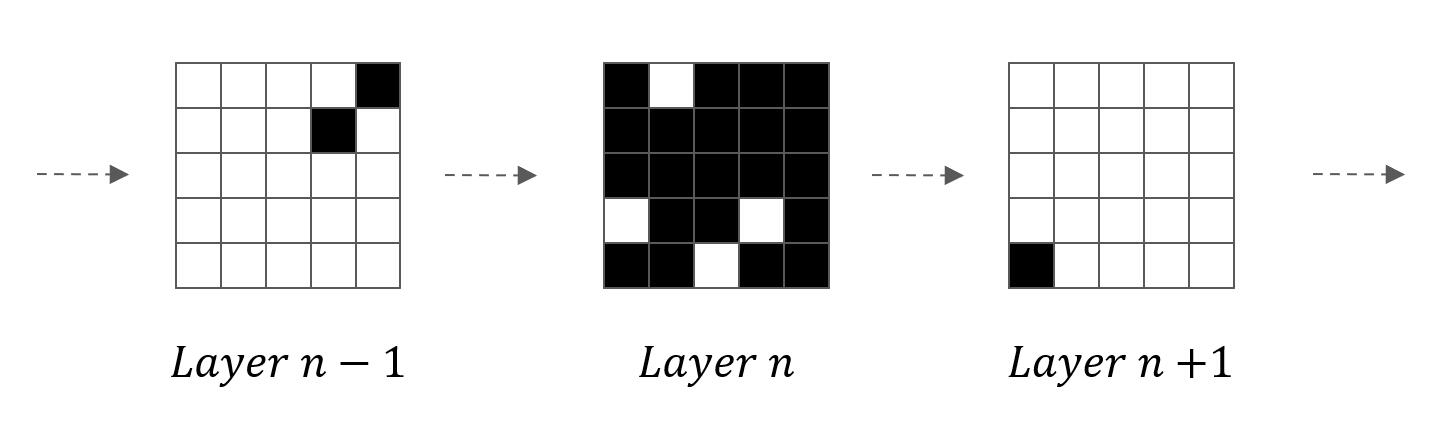
\includegraphics[width=0.85\linewidth]{char4_link_perturb_nogood.jpg}
    \caption{\label{char4:fig:link_perturb_nogood}最坏连接扰动应用于全局可能出现的截断现象。}
\end{figure}
\begin{figure}
    \centering
    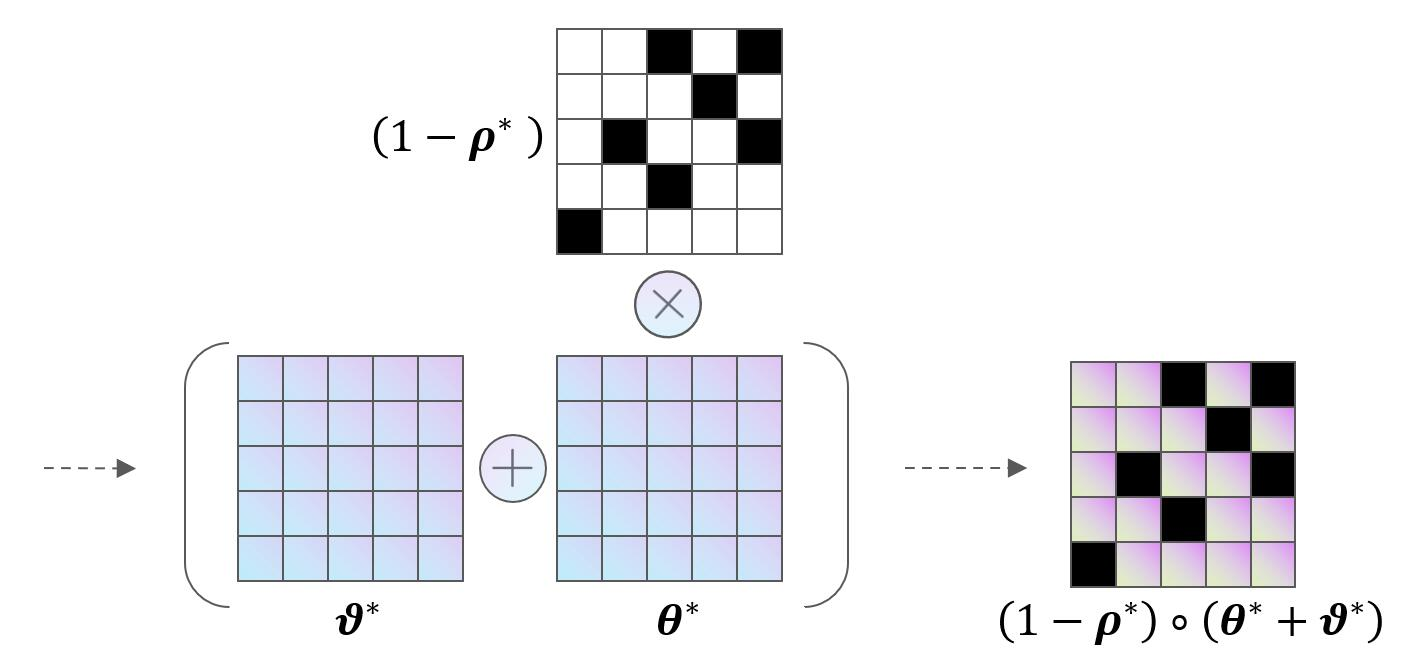
\includegraphics[width=0.85\linewidth]{char4_total_perturb.jpg}
    \caption{\label{char4:fig:total_pertub}最坏加性扰动和连接扰动在单层参数上的结合。}
\end{figure}
在获得全局最坏扰动$\boldsymbol \vartheta^*$和$\boldsymbol \rho^*$后,我们便可将加性扰动和连接扰动同时{应用于}神经网络参数上,
以期取得最大效果。其中连接扰动若应用于全局,容易出现即使设置连接失效阈值$p=0.1$也可能会导致连接扰动过于集中在某一层而使得神经网络中断的情况,
称之为“截断现象”,如\autoref{char4:fig:link_perturb_nogood}所示。
而加性扰动只要大小约束$\varepsilon$设置得当便不会出现这种情况,因此可将加性扰动直接应用于整个神经网络。
也就是说,在实际中,{连接扰动}将会分别应用于单层参数,配合加性扰动的具体做法如\autoref{char4:fig:total_pertub}所示,
对某层的卷积参数加上$\boldsymbol \vartheta^*$并点乘以$\left(\boldsymbol 1-\boldsymbol \rho^*\right)$便可得到经过最差加性和连接扰动后的
参数$\left(\boldsymbol 1-\boldsymbol \rho^*\right)\circ\left(\boldsymbol \theta+\boldsymbol \vartheta^* \right)$。

在实际仿真中不考虑锚点阈值小于0即对锚点数据集的扰动值无贡献度的数据,
设置分布式最坏扰动中锚点策略的扰动锚点阈值$\zeta_p$的取值范围为$\left[0,+\infty\right]$。
% 这里3-9不能设置为绝对值,因为负数是对贡献度的下降
以dSPUM-$l_{\mathrm{RLE}}$在$Pascal~Voc$上的mAP值变化为例,探索不同量级的扰动锚点阈值参数对性能和锚点数据集大小的的影响,实验结果如\autoref{char4:fig:zeta_p_1}和\autoref{char4:fig:zeta_p_2}所示。从图中可以看到扰动锚点阈值$\zeta_p$在数量级为1附近时,
性能趋于平缓且锚点数据集较小,是性能和成本极佳的平衡点,因此扰动锚点阈值$\zeta_p$设置为1。
加性扰动的大小约束$\varepsilon$和连接扰动的失效比例参数$p$在$\left[0,1\right]$中使用二分搜索分别获得最优值0.1和0.2。
\begin{figure}[htbp]
    \centering
    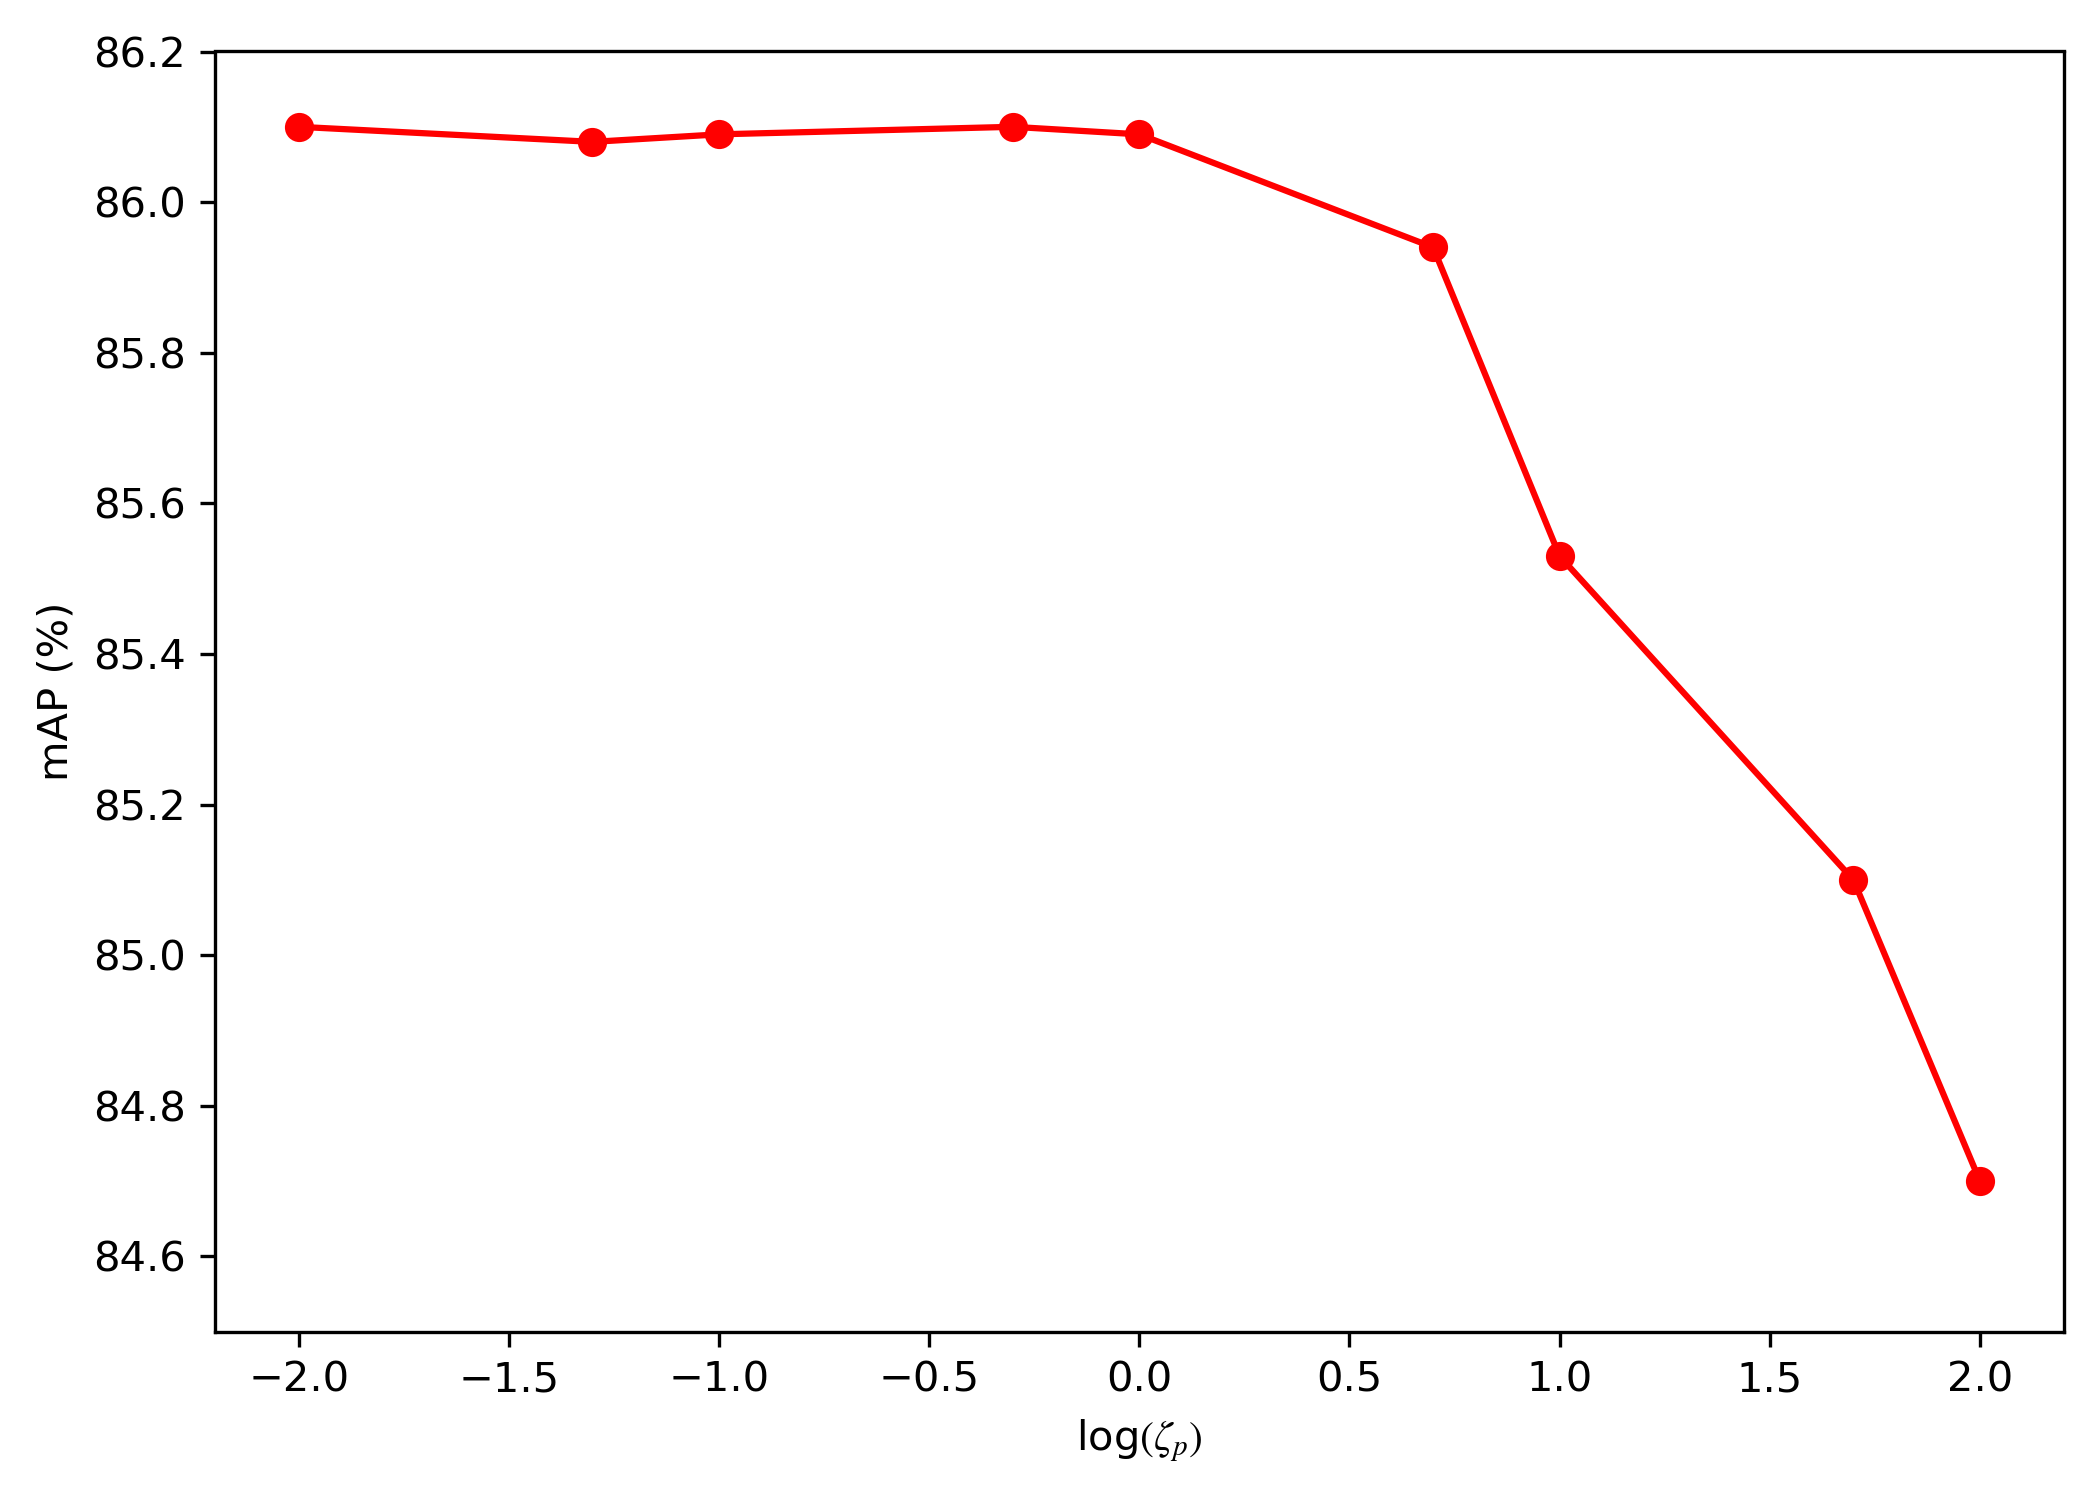
\includegraphics[width=0.7\linewidth]{char4_zeta_p_1.png}
    \caption{\label{char4:fig:zeta_p_1}在$Pascal~Voc$数据集上,PTR=10\%时
    不同量级的扰动锚点阈值参数$\zeta_p$对mAP值的影响。}
\end{figure}
\begin{figure}[htbp]
    \centering
    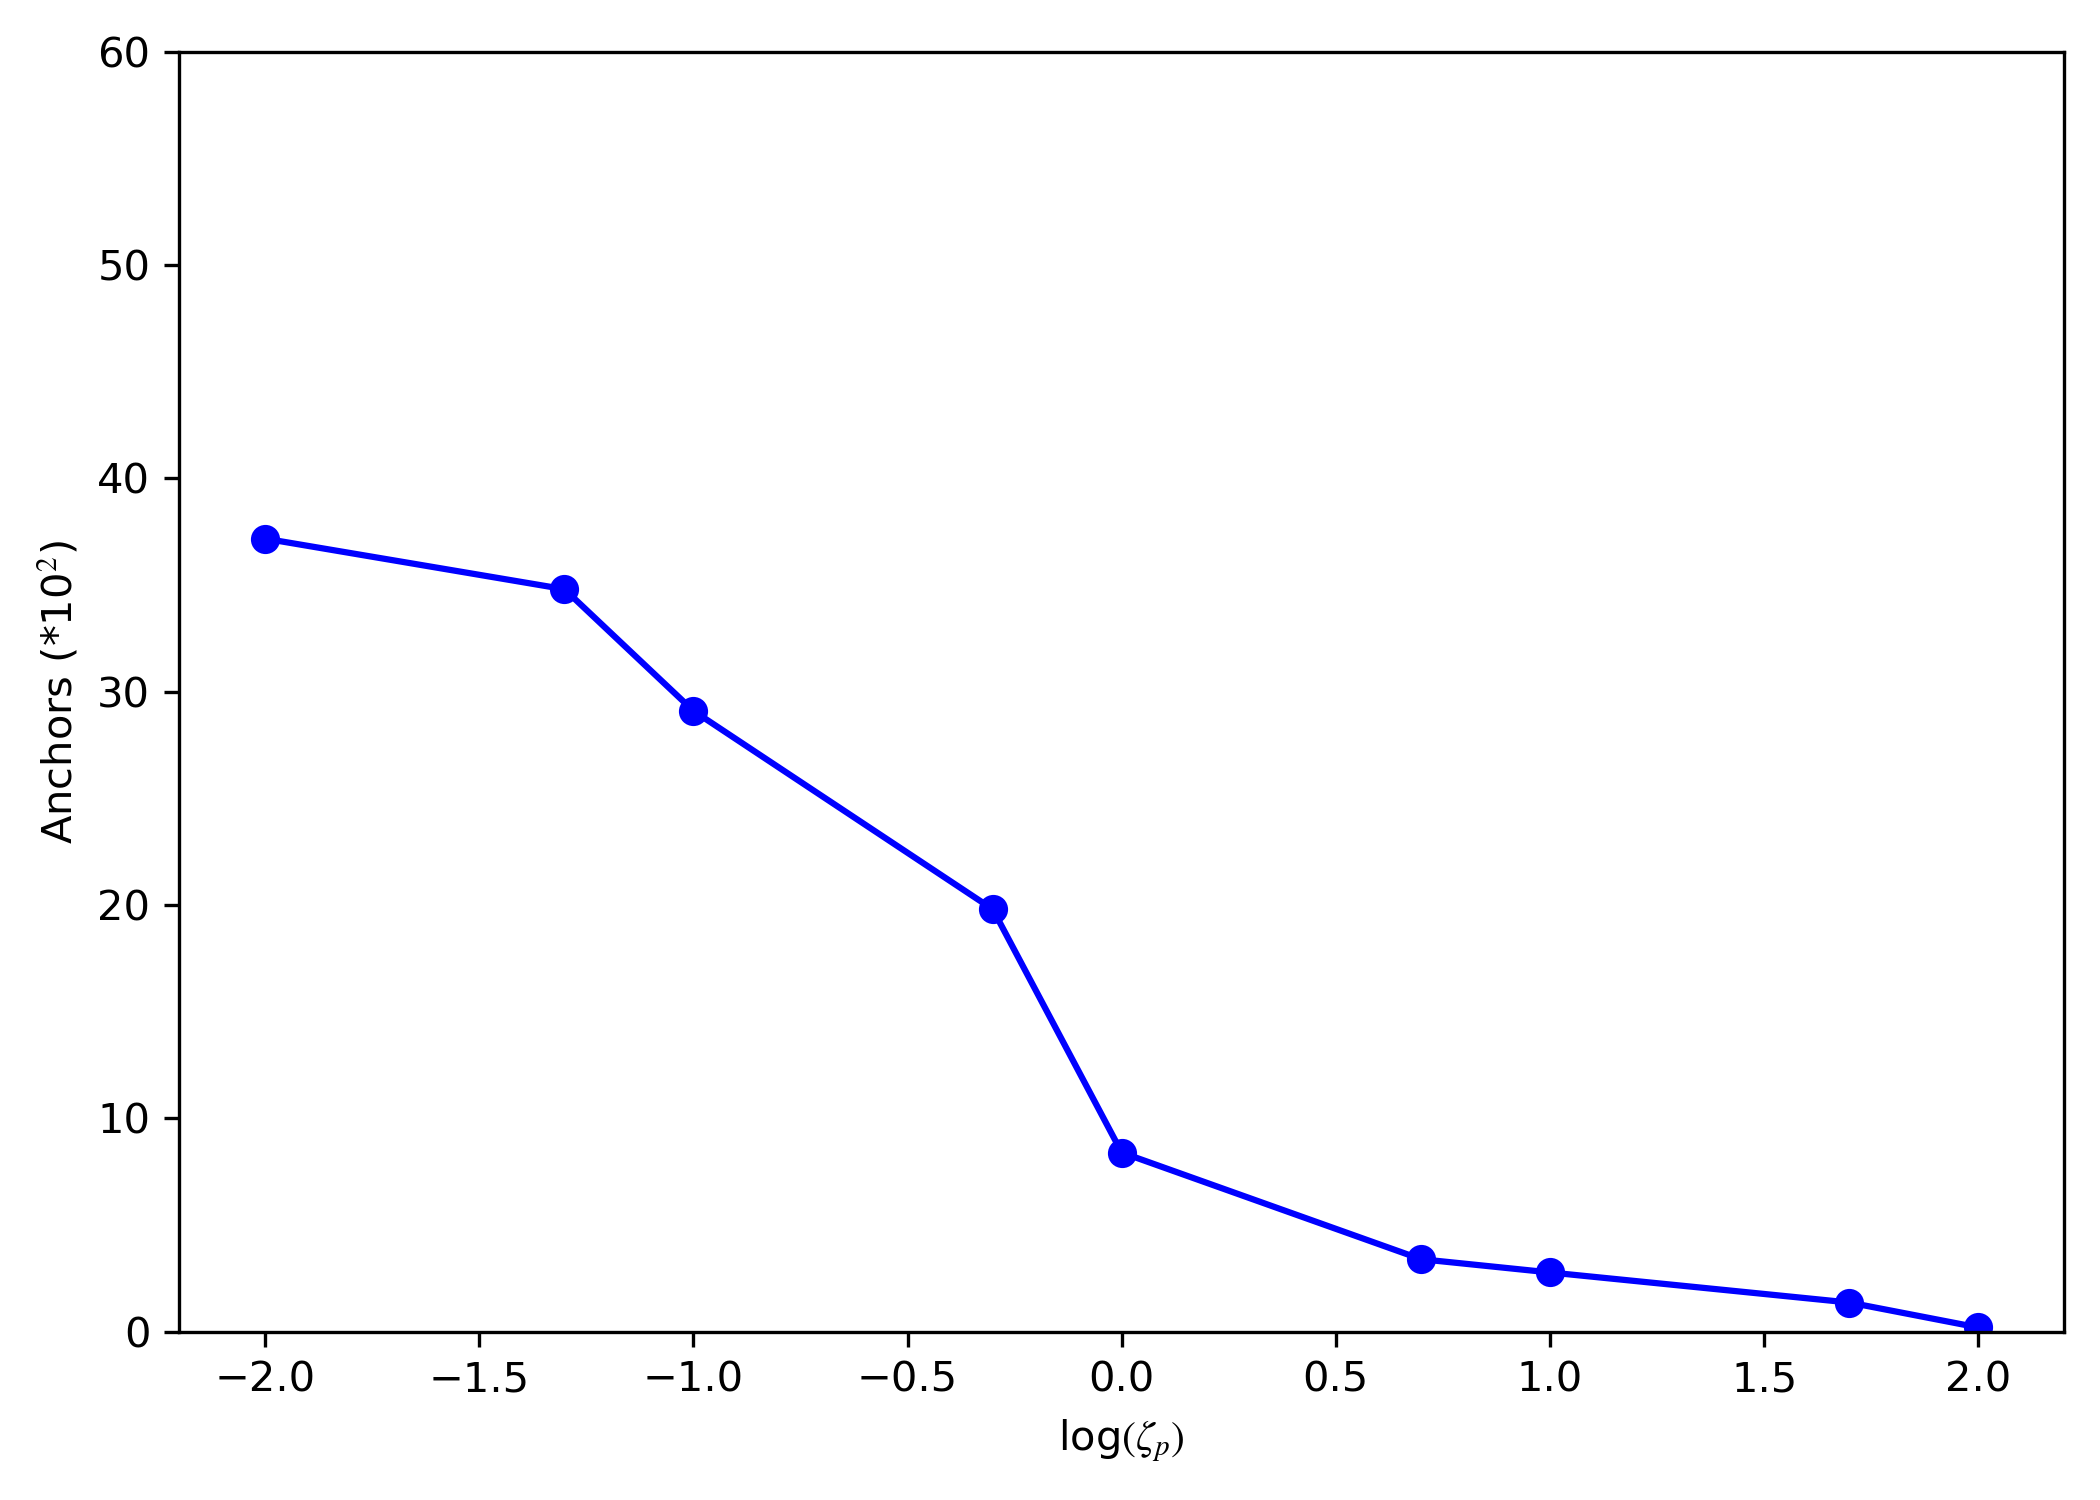
\includegraphics[width=0.7\linewidth]{char4_zeta_p_2.png}
    \caption{\label{char4:fig:zeta_p_2}在$Pascal~Voc$数据集上,PTR=10\%时
    不同量级的扰动锚点阈值参数$\zeta_p$对锚点数据集大小的影响。}
\end{figure}

\begin{figure}[htbp]
    \centering
    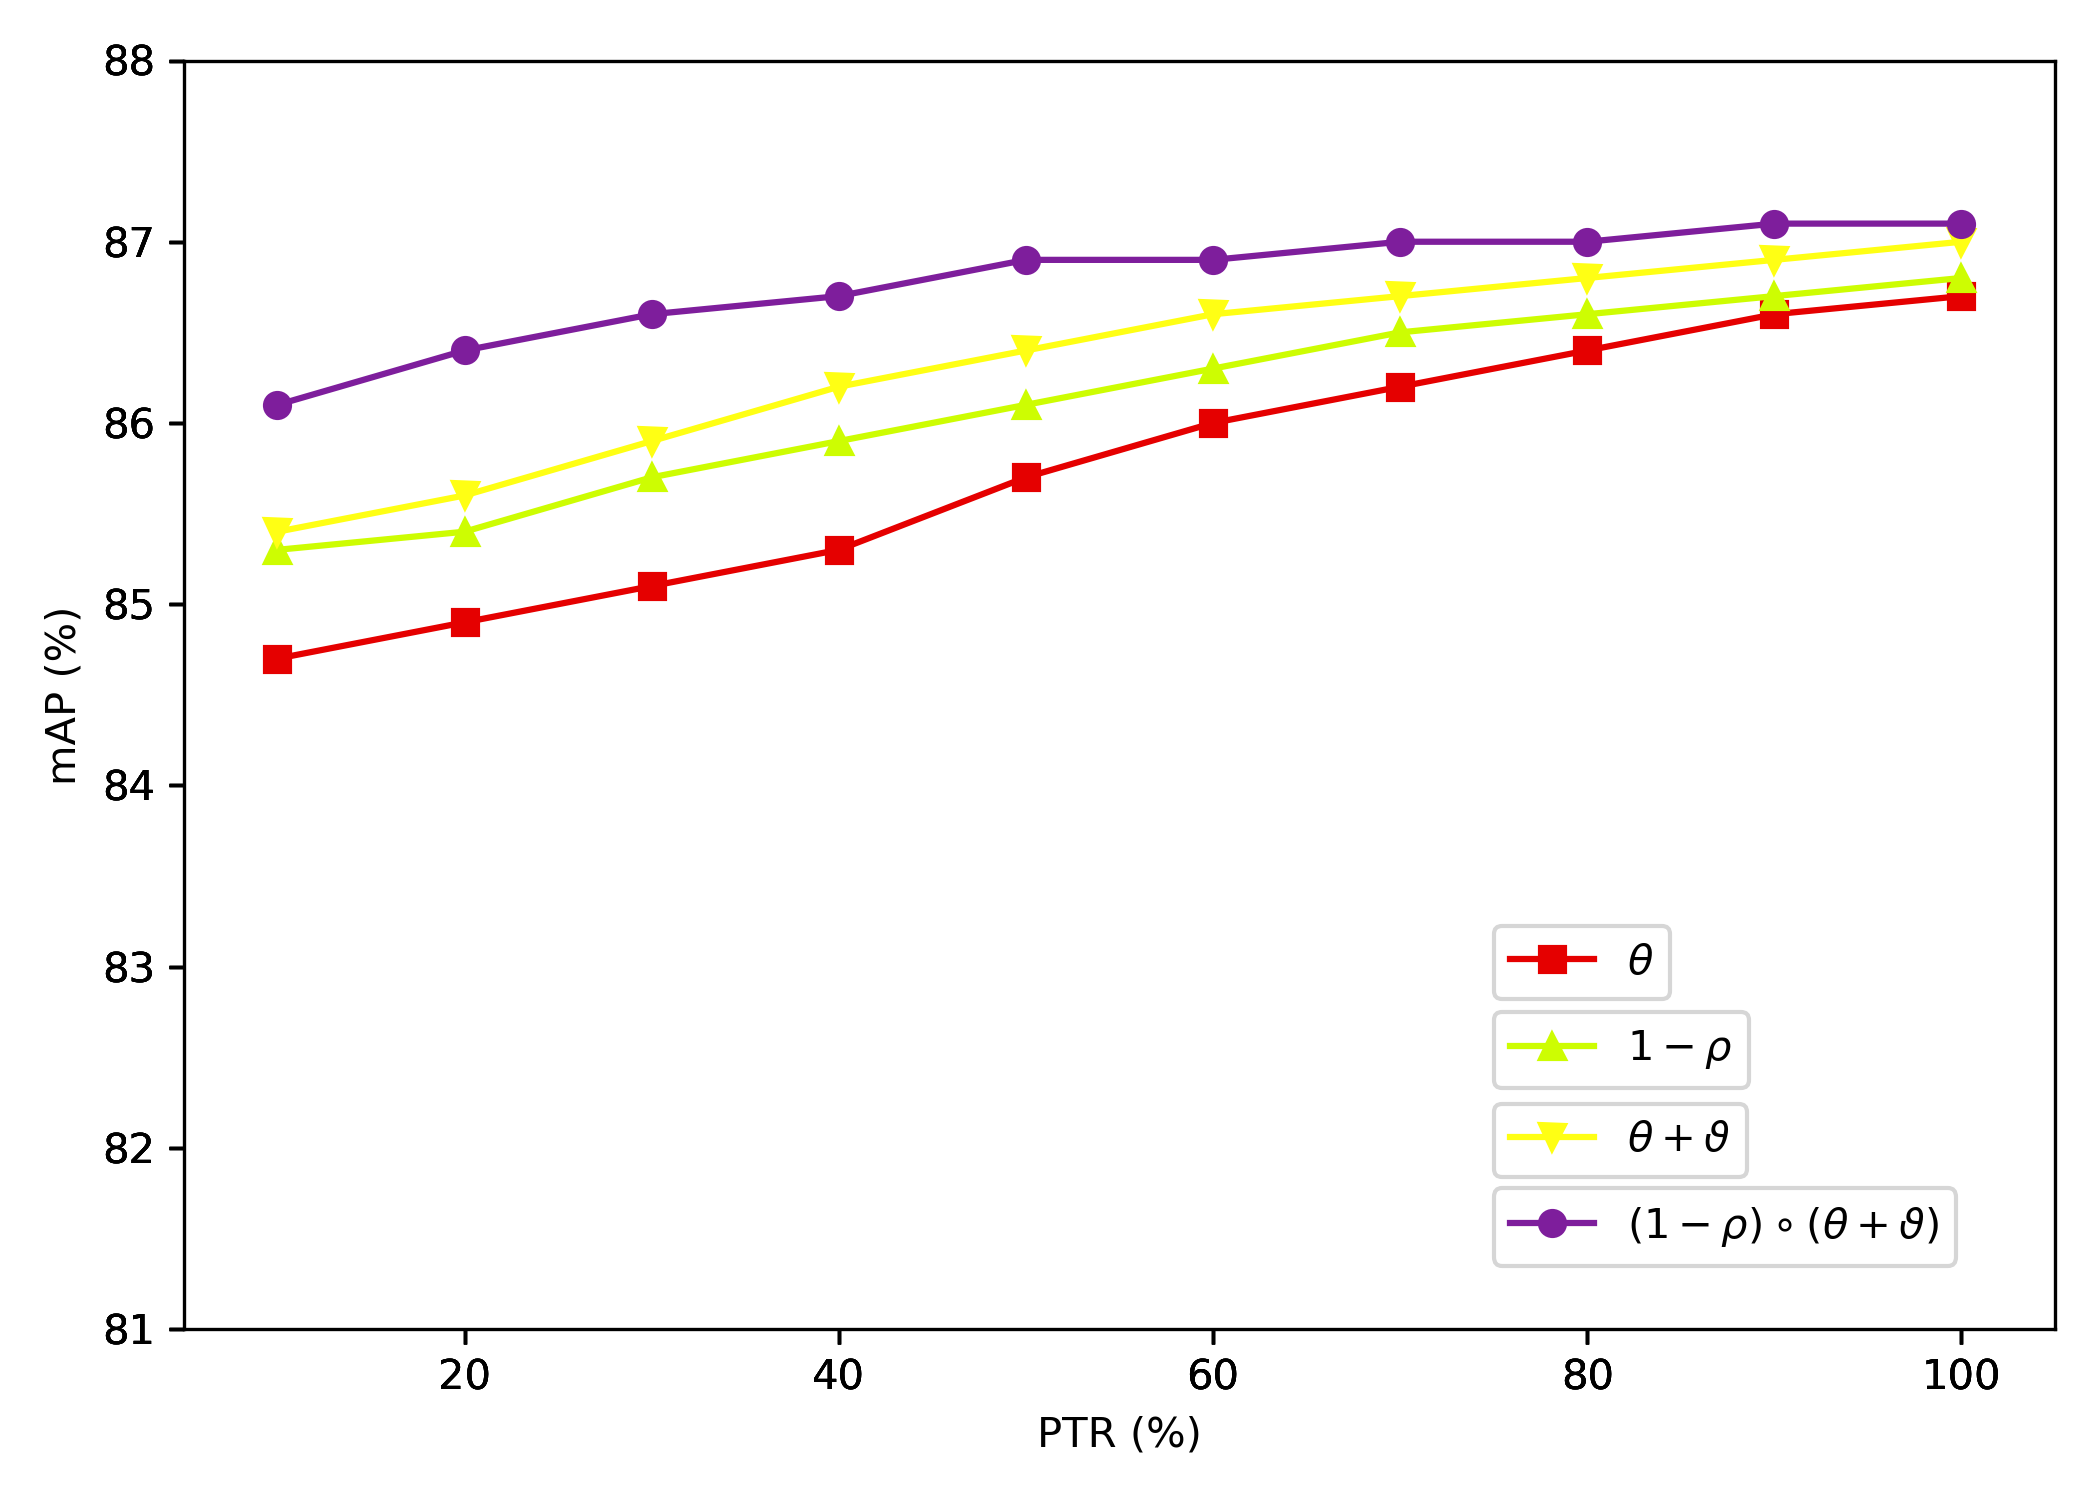
\includegraphics[width=0.7\linewidth]{char4_PTR_perturb.png}
    \caption{\label{char4:fig:PTR_perturb}在$Pascal~Voc$数据集上,不同PTR时不同类型的扰动对mAP值的影响。}
\end{figure}
参数确认后,为了展示不同类型的最坏扰动的效果,以dSPUM-$l_{\mathrm{RLE}}$算法为例探寻了在不同的PTR情况下,
加性扰动$\boldsymbol\theta+\boldsymbol \vartheta^*$,连接扰动$\boldsymbol 1-\boldsymbol \rho^*$和二者的结合
$\left(\boldsymbol 1-\boldsymbol \rho^*\right)\circ\left(\boldsymbol \theta+\boldsymbol \vartheta^* \right)$的优化效果。
结果如\autoref{char4:fig:PTR_perturb}所示,可以看到加性扰动和连接扰动的结合总是对算法有着更好的优化效果。


% 这里再想想怎么样说更通顺
在本章中,经过最坏扰动优化过的dPU算法的性能将在数据集$Cats$\&$Dogs\left(C\&D\right)$、$Tiny~~ImageNet\left(TI\right)$和$Flower$上进行验证,
其中为了适配dPU算法的单标签正例无标注分类场景,$Cats$\&$Dogs$中Cats类被设置为正类,
在$Tiny~~ImageNet$中选取类别鸡和鸟两类将鸡设为正类,在$Flower$选取玫瑰和百合两类并将玫瑰设置为正类,
并皆以特定PTR进行标注形成PU数据集,其数据集描述与锚点阈值$\zeta$将展示在\autoref{char4:tab:data_description}中。
而dSPUM算法的的性能分析仍在数据集$VOC,COCO,NUS,CUB,DOTA$和$UD$上进行,在各数据集上的参数设置与\autoref{char3:tab:data_description}相同并且使用\autoref{fig3:BDtest}中
表现最好的$l_{\mathrm{RLE}}$损失函数。
此外,在各数据集上的最优扰动锚点阈值$\zeta_p$,各扰动的最优约束参数,如加性扰动的大小约束$\varepsilon$和连接扰动的失效比例参数$p$,
将在各数据集上分别进行搜索得到最优值,搜寻结果如\autoref{char4:tab:perturb_reg}所示。
\begin{table}[htbp]
    \caption{\label{char4:tab:data_description}数据描述}
    \begin{tabularx}{\textwidth}{XXXXXX}
        \hline
        数据集 & 正样本数 & 负样本数 & 训练集大小 & 测试集大小 & $\zeta$ \\ \hline
        C\&D & 15000 & 15000 & 25000 & 5000 & 0.4 \\
        TI & 970 & 970 & 1552 & 488 & 0.7 \\
        Flower & 1030 & 1030 & 1596 & 464 & 0.4 \\ \hline
    \end{tabularx}
\end{table}
\begin{table}[htbp]
    \caption{\label{char4:tab:perturb_reg}各数据集扰动参数设置}
    \begin{tabularx}{\textwidth}{XXXX||XXXXXX}
        \hline
        算法 & \multicolumn{3}{c}{dPU} & \multicolumn{6}{c}{dSPUM} \\  \cline{1-10}
        数据集 & C$\&$D & TI & Flower & VOC & COCO & NUS & CUB & DOTA & UD \\ \hline
        $\zeta_p$ 
               & 0.10 & 0.50 & 0.50 & 1.00 & 1.00 & 0.50 & 5.00 & 1.00 & 1.00\\
        $\varepsilon$
               & 0.01 & 0.05 & 0.05 & 0.10 & 0.50 & 0.10 & 0.50 & 0.10 & 0.05 \\
        $p$    & 0.20 & 0.10 & 0.20 & 0.20 & 0.20 & 0.30 & 0.20 & 0.10 & 0.20 \\ \hline
    \end{tabularx}
\end{table}

为了探寻本文所提出的最坏扰动的优化能力,
本文将对dPU算法和dSPUM算法的参数分别施加以经过计算得到的最坏扰动$\boldsymbol 1-\boldsymbol \rho^*$,$\boldsymbol \theta+\boldsymbol \vartheta^*$
和将其二者结合的$\left(\boldsymbol 1-\boldsymbol \rho^*\right)\circ\left(\boldsymbol \theta+\boldsymbol \vartheta^*\right)$,
并综合比对未经过扰动的参数为$\boldsymbol \theta$的神经网络在上述各数据集上的性能从而分析出最坏扰动的优化性能。
最终结果如\autoref{char4:tab:Perturb_dPU}和\autoref{char4:tab:Perturb_dSSML}所示,从表中可以看出,
最坏加性扰动$\boldsymbol \vartheta^*$和最坏连接扰动$\boldsymbol 1-\boldsymbol \rho^*$都对算法有一定的提升效果,
但结合二者的$\left(\boldsymbol 1-\boldsymbol \rho^*\right)\circ\left(\boldsymbol \theta+\boldsymbol \vartheta^* \right)$效果最佳,
对dPU算法和dSPUM算法的表现都有较为明显的改进效果。
\begin{table}[htbp]
    \caption{\label{char4:tab:Perturb_dPU}基于不同扰动策略的dPU算法在PTR$=10\%$时在各数据集上的MCR(\%)表现。}
    \begin{tabularx}{\textwidth}{XXXXXXX}
        \hline
        &  \multicolumn{3}{c}{mAP(\%)} \\ \cline{2-4}
        扰动类型/数据集 & C\&D & TI & Flower \\ \hline
        $\boldsymbol \theta$                         & 5.9$\pm$0.2 & 4.1$\pm$0.4 & 3.5$\pm$0.3\\
        $\boldsymbol \theta+\boldsymbol \vartheta^*$ & 5.1$\pm$0.3 & 3.9$\pm$0.2 & 3.5$\pm$0.3\\
        $\boldsymbol 1-\boldsymbol \rho^*$           & 5.2$\pm$0.2 & 3.7$\pm$0.3 & 3.7$\pm$0.2\\
        $\left(\boldsymbol 1-\boldsymbol \rho^*\right)\circ\left(\boldsymbol \theta+\boldsymbol \vartheta^* \right)$
                                                     & \textbf{4.5$\pm$0.4} & \textbf{3.2$\pm$0.4} & \textbf{3.1$\pm$0.5}\\ \hline
    \end{tabularx}
\end{table}
% 对一下这里的数据
\begin{table}[htbp]
    \caption{\label{char4:tab:Perturb_dSSML}基于不同扰动策略的dSPUM算法在LTR$=10\%$时在各数据集上的mAP(\%)表现。}
    \begin{tabularx}{\textwidth}{XXXXXXX}
        \hline
        &   \multicolumn{6}{c}{mAP(\%)} \\ \cline{2-7}
        扰动类型/数据集 & VOC & COCO & NUS & CUB & DOTA & UD \\ \hline
        $\boldsymbol \theta$                         & 84.7$\pm$0.2 & 64.2$\pm$0.4 & 51.8$\pm$0.3 & 14.7$\pm$0.3 & 75.9$\pm$0.4 & 84.3$\pm$0.2\\
        $\boldsymbol \theta+\boldsymbol \vartheta^*$ & 85.3$\pm$0.3 & 64.6$\pm$0.2 & 51.9$\pm$0.3 & 15.1$\pm$0.3 & 76.9$\pm$0.2 & 84.8$\pm$0.3\\
        $\boldsymbol 1-\boldsymbol \rho^*$           & 85.4$\pm$0.2 & 64.7$\pm$0.3 & 52.1$\pm$0.2 & 15.2$\pm$0.4 & 76.5$\pm$0.3 & 84.7$\pm$0.3\\
        $\left(\boldsymbol 1-\boldsymbol \rho^*\right)\circ\left(\boldsymbol \theta+\boldsymbol \vartheta^* \right)$
                                                     & \textbf{86.1$\pm$0.4} & \textbf{65.3$\pm$0.4} & \textbf{53.0$\pm$0.5} & \textbf{15.8$\pm$0.6} & \textbf{77.8$\pm$0.5} & \textbf{85.1$\pm$0.4}\\ \hline
    \end{tabularx}
\end{table}

\section{本章小结}\label{Char4_Summary}
本节针对现有的随机扰动过于随机难以保证性能的问题,描述了一种针对神经网络计算出可以对其扰动效果最大化的最坏扰动约束项,其通过最大化扰动输出与原始输出之间的差距函数,得到使扰动后输出偏离最大的最坏扰动,
使得算法在最差情况下也能有较好的输出以提升算法在未见数据上的性能。
本文采用最坏加性噪声扰动和对模型连接进行覆盖的连接扰动以及二者的结合,对无法获取全部原始数据的分布式场景,提出了基于锚点数据的最坏扰动计算,以较小的传输代价逼近全局最坏扰动。
最终,对本文所提及的dPU和dSPUM算法施加以最差加性和最坏连接扰动以及二者的结合,经过在不同数据集上的仿真,
证实了最坏扰动能够提升算法对未见数据性能的优化效果,且加性扰动与连接扰动的结合具有更好的效果。

% 得看一下
% Chapter 5
\chapter{总结与展望}
本文基于数据的标注较为稀缺且不完整,数据受地理位置等因素制约收集并存储在不同的数据节点中的实际场景,主要研究了分布式网络中的正例无标注学习算法。在分布式优化过程中,网络中各节点之间在本地计算得到信息之后通过与邻居节点进行少量的信息交换,以去中心化的理念构建分布式学习系统去协同解决全局最优问题。本文的主要研究成果总结如下:

(1)针对分布于不同节点的正例无标注单标签数据,本文研究了基于一致性的分布式半监督正例学习算法dPU。
首先使用随机特征映射实现去中心化的核函数计算。
对本地正例数据和无标注数据分别设计相应损失函数并提出自适应的阈值设计方案,且使用锚点数据集使本地流形约束逼近全局性能,然后结合各节点的损失函数提出全局优化问题。
在基于一致性约束的前提下,使用交替乘子法对全局优化问题进行迭代求解得到全局最优解。
仿真结果表明,本文使用的随机特征映射在保证性能的同时节省了许多计算资源。
此外,本文所提出的分布式优化dPU算法可以得到与集中式cSPU算法相近的性能,并在多个数据集上和不同PU算法进行对比
验证了其优越性能。

(2)针对仅有部分数据被标注且已标注数据中仅有单个标签被标注为正的单正例无标注多标签数据,使用标签平滑、正类数量约束和预测输出约束等方法设计损失函数从未标注数据或未标注标签中提取有效信息以提升分类性能。
进一步地将损失函数拓展到分布式场景下,辅以基于锚点数据的流形约束得到对应全局优化问题。
使用分布式梯度下降法对各节点计算梯度后再通过中间变量传输到邻居节点进行融合,在这个过程中使用事件触发机制
约束了节点之间传递信息的频次。
仿真实验结果表明,事件触发机制在保持良好性能的同时大大降低了网络之间的通信成本,且相比于全监督的损失函数本文提出的
dSPUM算法使用极少的标注数量便可以达到接近的分类性能。
在不同数据集上和不同算法进行性能对比,通过弗得里曼检验(Friedman test)及其后续检验布氏检验(Bonferroni-Dunn test)
验证本文的算法的优越性能。

(3)针对本文所提的两种正例无标注学习算法进行进一步的优化。
在神经网络中采用最坏扰动对其结构进行最大化地破坏,以此最坏扰动约束项增强算法的鲁棒性。
使用锚点数据策略通过付出较小的通信代价,使得本地基于锚点数据的最坏扰动逼近全局最坏扰动,以此实现分布式最坏扰动。
在仿真实验中,通过对dPU算法和dSPUM算法施加以各类型的最坏扰动,证实了加性扰动与连接扰动结合的优越性,
并证明了最坏扰动对于半监督学习性能的优化能力。

% 想想还有啥展望
作为一种实用性极高的机器学习方法,半监督学习的应用领域非常广阔。
本文对正例无标注领域进行了探索,而实际半监督场景还有使用极小数据源的小样本学习、
使用候选标签集的部分标签学习以及模糊标签学习等方向值得研究。
此外,本文对于神经网络结构的探索较为浅显,在半监督领域,图神经网络和基于大规模数据预训练的transformer系列结构也是
后续可深入研究的方向。
对于分布式学习,本文探索了两种优化方法以及锚点技巧来进行信息传输,而如何进一步优化性能减轻通讯压力仍有待继续研究。
后续工作将关注分布式场景下更多领域的半监督学习,并结合多种深度神经网络进行研究。

